\documentclass{thesis}
%DIF LATEXDIFF DIFFERENCE FILE
%DIF DEL old.tex   Tue Jun 14 16:29:01 2016
%DIF ADD new.tex   Mon Aug 15 19:27:45 2016
\usepackage{thesis}
\usepackage{parskip}
\usepackage{hepnames}
\usepackage[printonlyused]{acronym}
\usepackage{ptdr-definitions}
\usepackage{slashed}
\usepackage{multirow}
\usepackage{amssymb}
\usepackage{import}
\usepackage{colortbl}
\usepackage{hhline}
\usepackage{feynmp}

%% You can set the line spacing this way
%\setallspacing{double}
%% or a section at a time like this
%\setfrontmatterspacing{double}


%% Define a few useful shorthands
\newcommand{\emu}{\Pe\Pgm}
\newcommand{\ee}{\Pe\Pe}
\newcommand{\mumu}{\Pgm\Pgm}
\newcommand{\mutau}{\Pgm\Pgth}
\newcommand{\etau}{\Pe\Pgth}
\newcommand{\tautau}{\Pgth\Pgth}

\newcommand{\WJets}{\ensuremath{\PW}{+}\text{jets}\xspace}
\newcommand{\mhmax}{\ensuremath{m_{\Ph}^{\text{max}}}\xspace}
\newcommand{\ttbar}{\ensuremath{\Pqt\Paqt}\xspace}
\newcommand{\ZToTauTau}{\ensuremath{\PZ\to\Pgt\Pgt}\xspace}
\newcommand{\HToTauTau}{\ensuremath{\PH\to\Pgt\Pgt}\xspace}

\renewcommand{\listfigurename}{List of figures}
\renewcommand{\listtablename}{List of tables}


\DeclareGraphicsRule{.1}{mps}{*}{}
\DeclareGraphicsRule{.2}{mps}{*}{}
\DeclareGraphicsRule{.3}{mps}{*}{}
\DeclareGraphicsRule{.4}{mps}{*}{}
\DeclareGraphicsRule{.5}{mps}{*}{}
\DeclareGraphicsRule{.6}{mps}{*}{}
\DeclareGraphicsRule{.7}{mps}{*}{}
\DeclareGraphicsRule{.8}{mps}{*}{}
\DeclareGraphicsRule{.9}{mps}{*}{}
\DeclareGraphicsRule{.10}{mps}{*}{}
\DeclareGraphicsRule{.11}{mps}{*}{}
\DeclareGraphicsRule{.12}{mps}{*}{}
\DeclareGraphicsRule{.13}{mps}{*}{}
\DeclareGraphicsRule{.14}{mps}{*}{}


%% PDF metadata
\makeatletter
\@ifpackageloaded{hyperref}{%
\hypersetup{%
hidelinks=true,
pdftitle = {Searches for invisibly decaying Higgs bosons with the CMS detector},
pdfsubject = {Patrick Dunne's PhD thesis},
pdfkeywords = {CMS, H, physics, LHC, Higgs},
pdfauthor = {\textcopyright\ Patrick Dunne},
linkcolor=black,
colorlinks=false
}
}{}
\makeatother

%% Define the thesis title and author
\title{Searches for invisibly decaying Higgs bosons with the CMS detector}
\author{Patrick James Dunne}

%% Start the document
%DIF PREAMBLE EXTENSION ADDED BY LATEXDIFF
%DIF UNDERLINE PREAMBLE %DIF PREAMBLE
\RequirePackage[normalem]{ulem} %DIF PREAMBLE
\RequirePackage{color}\definecolor{RED}{rgb}{1,0,0}\definecolor{BLUE}{rgb}{0,0,1} %DIF PREAMBLE
\providecommand{\DIFadd}[1]{{\protect\color{blue}\uwave{#1}}} %DIF PREAMBLE
\providecommand{\DIFdel}[1]{{\protect\color{red}\sout{#1}}}                      %DIF PREAMBLE
%DIF SAFE PREAMBLE %DIF PREAMBLE
\providecommand{\DIFaddbegin}{} %DIF PREAMBLE
\providecommand{\DIFaddend}{} %DIF PREAMBLE
\providecommand{\DIFdelbegin}{} %DIF PREAMBLE
\providecommand{\DIFdelend}{} %DIF PREAMBLE
%DIF FLOATSAFE PREAMBLE %DIF PREAMBLE
\providecommand{\DIFaddFL}[1]{\DIFadd{#1}} %DIF PREAMBLE
\providecommand{\DIFdelFL}[1]{\DIFdel{#1}} %DIF PREAMBLE
\providecommand{\DIFaddbeginFL}{} %DIF PREAMBLE
\providecommand{\DIFaddendFL}{} %DIF PREAMBLE
\providecommand{\DIFdelbeginFL}{} %DIF PREAMBLE
\providecommand{\DIFdelendFL}{} %DIF PREAMBLE
%DIF END PREAMBLE EXTENSION ADDED BY LATEXDIFF

\begin{document}

\begin{fmffile}{thesisfeynmandiags}
%% Define the un-numbered front matter (cover pages, rubrik and table of contents)
\begin{frontmatter}
%% Title
%??UPDATE THIS
\titlepage[of Imperial College London]%
{A dissertation submitted to Imperial College London\\
  for the degree of Doctor of Philosophy}

\newpage
The copyright of this thesis rests with the author and is made available under a Creative Commons
Attribution Non-Commercial No Derivatives licence. Researchers are free to copy, distribute or
transmit the thesis on the condition that they attribute it, that they do not use it for commercial
purposes and that they do not alter, transform or build upon it. For any reuse or redistribution,
researchers must make clear to others the licence terms of this work\DIFaddbegin \DIFadd{.
}\DIFaddend 

%% Abstract
\begin{abstract}%[\smaller \thetitle\\ \vspace*{1cm} \smaller {\theauthor}]
  %\thispagestyle{empty}
  Searches for invisibly decaying Higgs bosons using the Compact Muon Solenoid (CMS) detector at the CERN Large Hadron Collider (LHC) and their interpretations are described. These searches are motivated both by a desire to characterise the newly observed Higgs boson, and by the cosmological observation of very weakly interacting matter in the universe, which is called dark matter. In order to provide context for these searches, introductions to the Standard Model (SM) of particle physics and several extensions to the SM which incorporate dark matter are given.

The searches described in this thesis use data recorded in proton-proton collisions in 2012 and focus on the most sensitive mode, Vector Boson Fusion (VBF) production. The first search uses 19.5 \invfb\, of data promptly reconstructed in 2012 and results in an observed (expected) limit on the invisible branching fraction of the 125 \GeV Higgs boson, \BRinv, of 0.65 (0.49) at the 95\% confidence level (CL)~\cite{Chatrchyan:2014tja}. The second search uses 19.2 \invfb\,of data collected using triggers with looser thresholds and reconstructed later, in 2013. This search resulted in an observed (expected) limit on \BRinv of 0.57 (0.40) at the 95\% CL~\cite{CMS-PAS-HIG-14-038}.

Combinations of these searches with searches in other production channels are also described, the most sensitive of which results in an observed (expected) limit on \BRinv of 0.36 (0.30) at 95\% CL~\cite{CMS-PAS-HIG-15-012}. Projections of the sensitivity of these analyses in Run 2 and interpretations of their results as limits on various models of dark matter are also given~\cite{ourdmpaper}.
\end{abstract}


%% Declaration
\begin{declaration}
  This dissertation is the result of my own work. Where figures and results are taken from other sources this is indicated by an appropriate reference. Some figures referenced as from other sources were created by me, but appear in other public documents. 

The description of the analysis described in \ChapterRef{chap:prompt} follows \ReferenceRef{ARTICLE:CMSAN-12-403}, which includes elements of my work, and was made public in \ReferenceRef{Chatrchyan:2014tja}. Specifically, I was responsible for cross-checking the results of all the $\PW+$jets background estimations, I contributed to the development of the formula used to carry out the $\PZ+$jets background estimation, I calculated and cross-checked several of the systematic uncertainties, I produced plots of the discriminating variables for final publication, and I performed all limit setting and production of limit plots. 

I was the main analyser for the analysis described in \ChapterRef{chap:parked}, responsible for all steps of the analysis including trigger efficiency measurement, background estimation, systematic uncertainty studies and limit setting. The QCD background estimation method was developed and implemented collaboratively with other members of the Imperial College high energy physics (HEP) group. This work was made public in \ReferenceRef{CMS-PAS-HIG-14-038}.

I was also solely responsible for the combinations described in \ChapterRef{chap:comb}. For the interpretations of the VBF invisibly decaying Higgs boson searches as limits on dark mater models described in \ChapterRef{chap:interp} I worked collaboratively with theorists at Rutgers University and members of the Imperial College and Bristol University HEP groups. This work was made public in \ReferenceRef{ourdmpaper}.

As well as the work described in this thesis I have also carried out preparations for a search for VBF produced invisibly decaying Higgs bosons using Run 2 data from the LHC. These preparations have included measurements of the trigger efficiency for the triggers used in 2015 CMS data taking and comparisons of the kinematic distributions of signal and background events at the increased 13 TeV centre-of-mass energy used in Run 2 with those from Run 1, this work is currently under approval. Together with a new PhD student, I have also carried out a combination of the first Run 2 invisibly decaying Higgs boson searches in the VBF and ZH channels with those in Run 1, which is currently being approved for publication.


  \vspace*{1cm}
  \begin{flushright}
    Patrick James Dunne
  \end{flushright}
\end{declaration}


%% Acknowledgements
\begin{acknowledgements}
%??Stephanie, Mum, Dad rest of family
I would like to thank my wife Stephanie for her love and endless support and also for proofreading the entirety of this document. I'd also like to thank my parents Rebecca and Patrick, without whom I wouldn't have got to the position of being able to apply for a PhD.

%??Gavin, Dave, Anne Marie, Joao, Jim, Andrew, Nick all other colleagues
%??STFC, and IC
The help of my two supervisors Gavin Davies and David Colling has also been invaluable; thank you for always having your doors open when I needed advice. Thanks must also go to my colleagues on CMS and at Imperial, especially Anne-Marie Magnan, Joao Pela, Jim Brooke, Andrew Gilbert and Nick Wardle. I've learned a lot from our long discussions both on physics and on CMS politics. Finally, I would like to thank the Science Technology Facilities Council who funded this work, and Imperial College for all the resources they made available.
\end{acknowledgements}


%% Preface
%\begin{preface}
%\end{preface}

%% ToC
\tableofcontents

\renewcommand{\listfigurename}{List of figures}
\renewcommand{\listtablename}{List of tables}

\listoffigures
\listoftables

%% Strictly optional!
%\frontquote%
%{Writing in English is the most ingenious torture\\
%   ever devised for sins committed in previous lives.}%
%  {James Joyce}
\end{frontmatter}

%% Start the content body of the thesis
\begin{mainmatter}
  %% Actually, more semantic chapter filenames are better, like "chap-bgtheory.tex"
  \DIFaddbegin \cleardoublepage
  \pagenumbering{arabic}
\DIFaddend \chapter{Introduction and theory}
\label{chap:theory}
In order to describe the search for invisible decays of the Higgs boson (``Higgs to invisible''), it is necessary to describe the theory behind \DIFdelbegin \DIFdel{them }\DIFdelend \DIFaddbegin \DIFadd{it }\DIFaddend and the statistical techniques used in carrying out the search. This chapter will start with an introduction to the current best theory of particle physics, the \ac{SM}, focusing on the Higgs mechanism, before outlining the motivations behind, and some candidates for, physics \ac{BSM}, then concluding with a discussion of the statistics of hypothesis testing. Natural units, where $\hbar=c=1$, Einstein summation convention and Feynman slash notation are used throughout. \DIFdelbegin \DIFdel{Four vector }\DIFdelend \DIFaddbegin \DIFadd{Four-vector }\DIFaddend indices are labeled using Greek letters, and gauge group generators using Roman letters.

%??CHECK PLOT AXIS LABEL SIZES AND THAT LEGEND TERMS ARE STANDARD OR IN TEXT

\section{The standard model of particle physics}
\label{sec:SM}
The SM describes the interaction of the particles currently thought to be fundamental with the strong, weak and electromagnetic forces~\cite{GlashowPartialSymmetries,WeinbergModelOfLeptons,SalamNobelSymposium,eightfoldway}. Its predictions, which come from specifying the symmetries the theory respects and how they are broken, the particles in the theory, and 18 free parameters, have been tested in many different experiments, in some cases up to one part in a trillion \cite{PhysRevLett.100.120801}. However, it does face challenges, one example being that it does not describe \ac{DM}. 

The SM is a gauge invariant \ac{QFT}. To construct a QFT the symmetries that are respected by the theory and the fields it describes must be specified. The symmetries are important because of Noether's theorem, which states that for every continuously differentiable symmetry of the Lagrangian of a theory there is a corresponding conservation law~\cite{Noether:1918zz,doi:10.1080/00411457108231446}. An example of this is the conservation of energy, linear momentum and angular momentum, which result through Noether's theorem from Poincar\'e invariance, the invariance of the laws of physics under translations and rotations in space and time. In addition to giving rise to conservation laws, some types of symmetry lead to additional fields being required to preserve invariance\DIFdelbegin \DIFdel{, }\DIFdelend \DIFaddbegin \DIFadd{; }\DIFaddend this will be discussed further in \SectionRef{sec:gaugesym} \cite{PhysRev.96.191}.

Because particles correspond to the quantised excitations of fields, the fields that can be described by the QFT are constrained by the fundamental particles seen in nature. In order to add a new field an explanation for why the corresponding particle has not yet been observed must, therefore, be provided. Specifically, a scalar field corresponds to a \DIFdelbegin \DIFdel{spin zero }\DIFdelend \DIFaddbegin \DIFadd{spin-0 }\DIFaddend boson, spinor fields correspond to \DIFdelbegin \DIFdel{spin half }\DIFdelend \DIFaddbegin \DIFadd{spin-$\frac{1}{2}$ }\DIFaddend fermions, and vector fields correspond to \DIFdelbegin \DIFdel{spin 1 }\DIFdelend \DIFaddbegin \DIFadd{spin-1 }\DIFaddend bosons. We will now go through the particles observed in nature and how they are represented in the SM.

\subsection{Fundamental particles in nature}
There are two types of fundamental particles in nature, fermions and bosons. The fermions observed in nature that are currently thought to be fundamental are then divided into those which interact via the strong force (the quarks), and those which don't (the leptons). Both \DIFdelbegin \DIFdel{the }\DIFdelend quarks and leptons exist in two further types: charged and neutral in the case of the leptons, and \DIFdelbegin \DIFdel{up type and down type }\DIFdelend \DIFaddbegin \DIFadd{up-type and down-type }\DIFaddend in the case of the fermions. Another interesting feature of the fermions is that they are arranged in three generations. Each generation has one fermion of each type with the same quantum numbers as those in the other generations, except that the mass is different. \TableRef{tab:fermions} shows this structure.

\begin{table}
  \DIFdelbeginFL %DIFDELCMD < \caption{%%%
\DIFdelendFL \DIFaddbeginFL \caption[The fundamental fermions observed in nature separated into their three generations. Each particle shown also has an antiparticle with opposite charge and identical mass. The electric charges are given in units of the magnitude of the charge of the electron.]{\DIFaddendFL The fundamental fermions observed in nature separated into their three generations. Each particle shown also has an antiparticle with opposite charge and identical mass\DIFaddbeginFL \DIFaddFL{. The electric charges are given in units of the magnitude of the charge of the electron}\DIFaddendFL ~\cite{Agashe:2014kda}\DIFaddbeginFL \DIFaddFL{.}\DIFaddendFL }
  \label{tab:fermions}
  \begin{tabular}{ccccccc}
  \hhline{=======}
  &\multicolumn{3}{|c|}{Leptons}& \multicolumn{3}{c}{Hadrons} \\
  \cline{2-7}
  Generation & \multicolumn{1}{|c}{Particle} & Mass & \multicolumn{1}{c|}{Electric Charge} & Particle & Mass & Electric Charge \\
  \hhline{=======}
  \multirow{2}{*}{1} & \Pem & 511 \keV & -1 & \Pqu & 2.3 \MeV & $+\frac{2}{3}$ \\
  & \Pgne & $\sim$0 & 0 & \Pqd & 4.8 \MeV & $-\frac{1}{3}$ \\
  \hline
  \multirow{2}{*}{2} & \Pgmm & 105.7 \MeV & -1 & \Pqc & 1.275 \GeV & $+\frac{2}{3}$ \\
  & \Pgngm & $\sim$0 & 0 & \Pqs & 95 \MeV & $-\frac{1}{3}$ \\
  \hline
  \multirow{3}{*}{2} & \Pgtm & 1.777 \GeV & -1 & \Pqt & 173.2 \GeV & $+\frac{2}{3}$ \\
  & \Pgngt & $\sim$0 & 0 & \Pqb & 4.18 \GeV & $-\frac{1}{3}$ \\
  \hhline{=======}
  \end{tabular}
\end{table}

The bosons in nature also exist in two types. The first type are vector bosons, which mediate the three fundamental interactions described by the SM. The vector bosons are summarised in \TableRef{tab:bosons}, where it can be seen that their masses are very different, the photon and the eight gluons being massless, while the \PWpm and \PZ bosons are massive. As we will see in \SectionRef{sec:ssb}, explaining these masses requires the Higgs mechanism~\cite{Englert:1964et,Higgs:1964ia,Higgs:1964pj,Guralnik:1964eu,Higgs:1966ev,Kibble:1967sv}. The Higgs mechanism also gives rise to the other type of boson seen in nature, the scalar Higgs boson. In order to see how all of the above particles are represented in the SM, an introduction to gauge theories is necessary.

\begin{table}
  \DIFdelbeginFL %DIFDELCMD < \caption{%%%
\DIFdelendFL \DIFaddbeginFL \caption[The fundamental vector bosons observed in nature separated by the force which they mediate. The electric charges are given in units of the magnitude of the charge of the electron.]{\DIFaddendFL The fundamental vector bosons observed in nature separated by the force which they mediate\DIFaddbeginFL \DIFaddFL{. The electric charges are given in units of the magnitude of the charge of the electron}\DIFaddendFL ~\cite{Agashe:2014kda}.}
  \label{tab:bosons}
  \begin{tabular}{lccc}
    \hline
    \hline
    Force & Particle & Mass & Electric Charge \\
    \hhline{====}
    Electromagnetism & \Pgg & 0 & 0 \\
    \hline
    \multirow{2}{*}{Weak} & \PWpm & 80.4 \GeV & $\pm 1$ \\
    \cline{2-4}
    & \PZ & 91.2 \GeV & 0 \\
    \hline
    Strong & g & 0 & 0 \\
    \hline
    \hline
  \end{tabular}
\end{table}

\subsection{Introduction to gauge theories}
\label{sec:gaugesym}
Gauge symmetries are local transformations, i.e. the transformation can be different at different points in space and time. To see the effect of imposing such a symmetry on a theory, consider imposing local invariance under U(1) transformations on the Dirac Lagrangian for a fermion, $\psi$, with mass, $m$:
\begin{equation}
  \label{eq:globaldiraclagrangian}
  \mathcal{L}=i\bar{\psi}\slashed{\partial}\psi-m\bar{\psi}\psi~\cite{griffiths2008introduction}.
\end{equation}

This Lagrangian is invariant under a global $U(1)$ transformation $\psi\rightarrow e^{iq\theta}\psi$, where \DIFdelbegin \DIFdel{q }\DIFdelend \DIFaddbegin \DIFadd{$q$ }\DIFaddend and $\theta$ are constant. However, if the $U(1)$ transformation is local i.e. $\theta$ is a function of spacetime position the Lagrangian is no longer invariant and transforms as:
\begin{equation}
  \label{eq:gaugeviolating}
  \mathcal{L}\rightarrow\mathcal{L}-q(\partial_{\mu}\theta)\bar{\psi}\gamma^{\mu}\psi.
\end{equation}

In order to restore invariance, a vector field, $A_{\mu}$, referred to as a gauge field or gauge boson, which transforms as $A_{\mu}\rightarrow A_{\mu}+\partial_{\mu}\theta$ and has an interaction with the fermion field:
\begin{equation}
  \mathcal{L}_{int}=q(\bar{\psi}\gamma^{\mu}\psi) A_{\mu},
\end{equation}
 can be added to the theory. The interaction term of the new gauge field transforms as:
\begin{equation}
  \mathcal{L}_{int}\rightarrow \mathcal{L}_{int}+q(\partial_{\mu}\theta)\bar{\psi}\gamma^{\mu}\psi,
\end{equation}
which precisely cancels the non-gauge invariance seen in \EquationRef{eq:gaugeviolating}. Assuming the new gauge field to be massless the Lagrangian is now:
\begin{equation}
  \label{eq:diraclag}
  \mathcal{L}=i\bar{\psi}\slashed{\partial}\psi-m\bar{\psi}\psi+q(\bar{\psi}\gamma^{\mu}\psi) A_{\mu}-\frac{1}{4}F_{\mu\nu}F^{\mu\nu},
\end{equation}
where $F_{\mu\nu}$ is the field strength tensor of the vector field. For a gauge boson from a general gauge group $F_{\mu\nu}$ is written as:
\begin{equation}
F_{\mu\nu}^a=\partial_{\mu}A_{\nu}^a-\partial_{\nu}A_{\mu}^a+gf_{abc}A_{\mu}^{b}A_{\nu}^{c},
\end{equation}
where $f^{abc}$ are the structure constants of the gauge group, which are a representation of the commutation relations between the group's generators. For $U(1)$, which only has one self-commuting generator, the single structure constant is 0. However, for non-Abelian gauge groups (i.e. those with non-commuting generators) they can be non-zero causing the $F_{\mu\nu}F^{\mu\nu}$ term in the Lagrangian to include self-interaction terms of the vector bosons.

\EquationRef{eq:diraclag} can be rewritten as:
\begin{equation}
  \label{eq:localdiraclagrangian}
  \mathcal{L}=i\bar{\psi}\gamma^{\mu}\mathcal{D}_{\mu}\psi-m\bar{\psi}\psi-\frac{1}{4}F_{\mu\nu}F^{\mu\nu},
\end{equation}
where $\mathcal{D}_{\mu}=\partial_{\mu}+iqA_{\mu}$ and is referred to as the covariant derivative. Comparing \EquationRef{eq:globaldiraclagrangian} and \EquationRef{eq:localdiraclagrangian} it can be seen that to go from a globally invariant Lagrangian to a locally invariant one we have substituted the normal spacetime derivative for the covariant derivative and added the free term of the vector field.

In the case of $U(1)$ transformations, which have one degree of freedom \DIFdelbegin \DIFdel{so }\DIFdelend \DIFaddbegin \DIFadd{and therefore }\DIFaddend can be described by one parameter \DIFdelbegin \DIFdel{, in the above case $\theta$}\DIFdelend \DIFaddbegin \DIFadd{($\theta$ in the case above)}\DIFaddend , in order to make the Lagrangian locally invariant one interacting gauge boson had to be added. This correspondence between the number of degrees of freedom and the number of gauge bosons holds generally. For each degree of freedom of a group's transformations there exists a generator of the group, and for each generator one interacting gauge boson must be added to achieve local invariance.

%give SM gauge group and fermion and vector representations 
\subsection{The SM gauge group and fundamental particle representations}
\label{sec:smgauge}
The \ac{SM} is locally gauge invariant under the group \DIFdelbegin \DIFdel{$SU\left(3\right)_{C}\otimes SU\left(2\right)_{L}\otimes U\left(1\right)_{Y}$. $SU\left(3)\right)_{C}$ }\DIFdelend \DIFaddbegin \DIFadd{$SU\!\left(3\right)_{C}\otimes SU\!\left(2\right)_{L}\otimes U\!\left(1\right)_{Y}$. $SU\!\left(3\right)_{C}$ }\DIFaddend is the group governing the strong force interactions which couple to colour charge, C. \DIFdelbegin \DIFdel{$SU\left(2\right)_{L}$}\DIFdelend \DIFaddbegin \DIFadd{$SU\!\left(2\right)_{L}$}\DIFaddend , which couples to \DIFdelbegin \DIFdel{left handed }\DIFdelend \DIFaddbegin \DIFadd{left-handed }\DIFaddend fermions, L, and \DIFdelbegin \DIFdel{$U\left(1\right)_{Y}$}\DIFdelend \DIFaddbegin \DIFadd{$U\!\left(1\right)_{Y}$}\DIFaddend , which couples to weak hypercharge, $Y$ are the groups governing the electroweak interactions. The weak hypercharge of any given particle is:
\begin{equation}
  Y=2(Q-T_{3}),
\end{equation}
where $Q$ is the electric charge, and $T_{3}$ is the third component of the weak isospin, which is $\pm\frac{1}{2}$ for \DIFdelbegin \DIFdel{left handed }\DIFdelend \DIFaddbegin \DIFadd{left-handed }\DIFaddend fermions, and zero for all other particles.

 Fermions in the SM are \DIFdelbegin \DIFdel{spin half }\DIFdelend \DIFaddbegin \DIFadd{spin-half }\DIFaddend spinor representations of these symmetry groups. These spinors can be split into chirally \DIFdelbegin \DIFdel{left and right handed }\DIFdelend \DIFaddbegin \DIFadd{left- and right-handed }\DIFaddend components using the projection operators $P_{\substack{L \\R}}=\frac{1}{2}(1\mp \gamma^{5})$. Chirally left and \DIFdelbegin \DIFdel{right handed }\DIFdelend \DIFaddbegin \DIFadd{right-handed }\DIFaddend fermions transform differently under \DIFdelbegin \DIFdel{$SU\left(2\right)_{L}$. The right handed }\DIFdelend \DIFaddbegin \DIFadd{$SU\!\left(2\right)_{L}$. The right-handed }\DIFaddend spinors are not charged under \DIFdelbegin \DIFdel{$SU\left(2\right)_{L}$ }\DIFdelend \DIFaddbegin \DIFadd{$SU\!\left(2\right)_{L}$ }\DIFaddend and thus are represented as a singlet, while the \DIFdelbegin \DIFdel{left handed }\DIFdelend \DIFaddbegin \DIFadd{left-handed }\DIFaddend spinors transform as a doublet.

The first generation of leptons can, therefore, be written as:
\begin{equation}
  \psi_{1}=\Pe_{R},\,\psi_{2}=L=\left(\begin{array}{c} \Pgne \\ \Pe_{L}\end{array}\right).
\end{equation}
The SM treats neutrinos as massless and has no \DIFdelbegin \DIFdel{right handed }\DIFdelend \DIFaddbegin \DIFadd{right-handed }\DIFaddend neutrino. Similarly the first generation of quarks can be written as:
\begin{equation}
  \psi_{3}=\Pqu_{R},\,\psi_{4}=\Pqd_{R},\,\psi_{5}=\left(\begin{array}{c} \Pqu_{L} \\ \Pqd_{L}\end{array}\right).
\end{equation}

As we saw in \SectionRef{sec:gaugesym} gauge symmetries in theories with fermions require the addition of an interacting vector boson per symmetry generator to preserve gauge invariance. \DIFdelbegin \DIFdel{$SU\left(3\right)_{C}$ }\DIFdelend \DIFaddbegin \DIFadd{$SU\!\left(3\right)_{C}$ }\DIFaddend has eight generators whose eight vector bosons, $G_{a\mu}$, correspond to the eight physical gluons of \ac{QCD}, which mediate the strong interaction. \DIFdelbegin \DIFdel{$SU\left(2\right)_{L}$ }\DIFdelend \DIFaddbegin \DIFadd{$SU\!\left(2\right)_{L}$ }\DIFaddend has three generators whose three vector bosons, $\PW^{i}_{\mu}$, mix with the one vector boson from \DIFdelbegin \DIFdel{$U\left(1\right)_{Y}$}\DIFdelend \DIFaddbegin \DIFadd{$U\!\left(1\right)_{Y}$}\DIFaddend , $B_{\mu}$ unifying the electromagnetic and weak forces into one electroweak force. The physical states that result are:
\begin{equation}
  \begin{split}
  \PWpm_{\mu}=\frac{1}{\sqrt{2}}\left(\PW^{1}_{\mu}\mp i\PW^{2}_{\mu}\right) \\
  \PZ_{\mu}=\DIFdelbegin \DIFdel{cos}\DIFdelend \DIFaddbegin \DIFadd{\cos}\DIFaddend \left(\theta_{W}\right)\PW^{3}_{\mu}\DIFdelbegin \DIFdel{-sin}\DIFdelend \DIFaddbegin \DIFadd{-\sin}\DIFaddend \left(\theta_{W}\right)B_{\mu} \\
  A_{\mu}=\DIFdelbegin \DIFdel{sin}\DIFdelend \DIFaddbegin \DIFadd{\sin}\DIFaddend \left(\theta_{W}\right)\PW^{3}_{\mu}+\DIFdelbegin \DIFdel{cos}\DIFdelend \DIFaddbegin \DIFadd{\cos}\DIFaddend \left(\theta_{W}\right)B_{\mu},
  \end{split}
\end{equation}
where $\theta_{W}$ is the Weinberg (weak) mixing angle and $A_{\mu}$ is the photon field. Also, as described in \SectionRef{sec:gaugesym} the interaction between these vector bosons and the fermion fields occurs through their presence in the covariant derivative, and interactions between the vector bosons occur because \DIFdelbegin \DIFdel{$SU\left(3\right)_{C}$ and $SU\left(2\right)_{L}$ }\DIFdelend \DIFaddbegin \DIFadd{$SU\!\left(3\right)_{C}$ and $SU\!\left(2\right)_{L}$ }\DIFaddend are non-Abelian.

Now let us try to construct a Lagrangian for these fields. First ignoring the masses we find:
\begin{equation}
  \mathcal{L}=i\bar{\psi}_{i}\slashed{\mathcal{D}}\psi_{i}-\frac{1}{4}F_{\mu\nu j}F^{\mu\nu}_{j},
\end{equation}
where the sum over all $\psi$ also includes the second and third generations, $F_{\mu\nu j}F^{\mu\nu}_{j}$ is a sum of the free terms of all the SM gauge bosons and $\mathcal{D}$ is the SM covariant derivative:
\begin{equation}
  \mathcal{D_{\mu}}=\partial_{\mu}+ig_{1}\frac{Y}{2}B_{\mu}+ig_{2}\frac{\tau_{i}}{2}W_{\mu}^{i}+ig_{3}\frac{\lambda_{a}}{2}G_{\mu}^{a},
\end{equation}
with Y being the constant generator of \DIFdelbegin \DIFdel{$U\left(1\right)$}\DIFdelend \DIFaddbegin \DIFadd{$U\!\left(1\right)$}\DIFaddend , $\tau_{i}$ the generators of \DIFdelbegin \DIFdel{$SU\left(2\right)_{L}$}\DIFdelend \DIFaddbegin \DIFadd{$SU\!\left(2\right)_{L}$}\DIFaddend , $\lambda_{a}$ the generators of \DIFdelbegin \DIFdel{$SU\left(3\right)_{C}$ }\DIFdelend \DIFaddbegin \DIFadd{$SU\!\left(3\right)_{C}$ }\DIFaddend and $g_{i}$ the coupling constants of the fields. It should be noted that $\frac{g_{1}}{g_{2}}$ is equal to $\tan\left(\theta_{W}\right)$.

When we try to include mass a problem occurs. We know that some of the fermions have mass, and consequently we should have fermion mass terms of the form:
\begin{equation}
  \begin{split}
    \mathcal{L}_{m_{f}}&=-m_{f}\bar{f}{f} \\
    &=-m_{f}\bar{f}\left[\frac{1}{2}\left(1-\gamma^{5}\right)+\frac{1}{2}\left(1+\gamma^{5}\right)\right]f \\
    &=-m_{f}\left(\bar{f}_{R}f_{L}+\bar{f}_{L}f_{R}\right),
  \end{split}
\end{equation}
in our Lagrangian. However, as the left and \DIFdelbegin \DIFdel{right handed }\DIFdelend \DIFaddbegin \DIFadd{right-handed }\DIFaddend fields do not transform in the same way under \DIFdelbegin \DIFdel{$SU\left(2\right)_{L}$}\DIFdelend \DIFaddbegin \DIFadd{$SU\!\left(2\right)_{L}$}\DIFaddend , this term breaks the gauge symmetry of the Lagrangian and can't be present. 

A similar problem occurs for vector fields. In \SectionRef{sec:gaugesym} we didn't consider the mass term of these vector fields:
\begin{equation}
  \label{eq:vectorlagrangian}
  \mathcal{L}_{m_V}=\frac{1}{2}m_{V}^{2}A_{\mu}A^{\mu},
\end{equation}
which is not gauge invariant, so it is not possible to include the massive vector bosons on their own in gauge invariant theories either. The additional piece of the SM required to allow particles to have mass is the Higgs mechanism.

\subsection{Spontaneous symmetry breaking and the Higgs mechanism}
\label{sec:ssb}
%Introduce SSB
The Higgs mechanism is a form of spontaneous symmetry breaking~\cite{Englert:1964et,Higgs:1964ia,Higgs:1964pj,Guralnik:1964eu,Higgs:1966ev,Kibble:1967sv}. A symmetry is said to be spontaneously broken when the Lagrangian remains invariant while the vacuum state, i.e. that with lowest energy, does not~\cite{griffiths2008introduction}. Terms of the Lagrangian which are not gauge invariant can then be incorporated into the theory by adding a field which has a non-zero vacuum expectation value and coupling it to the other fields present in the desired term. For the Higgs mechanism this field is a complex scalar \DIFdelbegin \DIFdel{$SU\left(2\right)_{L}$ }\DIFdelend \DIFaddbegin \DIFadd{$SU\!\left(2\right)_{L}$ }\DIFaddend doublet, $\phi$, called the Higgs field:
\begin{equation}
\phi=\left(\begin{array}{c}\phi^+ \\ \phi^0 \end{array}\right).
\end{equation}
The main part of the Higgs field Lagrangian is:
\begin{equation}
  \label{eq:higlag}
\mathcal{L}=T-V=\left(\mathcal{D}_{\mu}\phi\right)^{\dag}\left(\mathcal{D}^{\mu}\phi\right)+\mu^{2}\phi^{\dag}\phi-\lambda\left(\phi^{\dag}\phi\right)^{2},
\end{equation}
Where the first two terms on the right hand side make up the kinetic part of the Higgs field Lagrangian, $T$, and the third term is the Higgs field potential, $V$. For $\mu^{2}>0$, the values of the Higgs field which minimise the Lagrangian are  non-zero and form a circle in the phase space of $\phi$. All of these minima are equivalent and a particular minimum can be chosen with no physical effect. By convention we choose the following minimum:
\begin{equation}
  \bra{0}\phi\ket{0}=\left(\begin{array}{c} 0 \\ \sqrt{\frac{\mu^{2}}{2\lambda}} \end{array}\right)=\frac{1}{\sqrt{2}}\left(\begin{array}{c} 0 \\ v \end{array}\right).
\end{equation}
Next we consider small perturbations around this minimum. Ignoring perturbations that can be set to zero by gauge freedom \DIFaddbegin \DIFadd{this }\DIFaddend gives:
\begin{equation}
  \phi=\left(\begin{array}{c}0 \\ v+H \end{array}\right).
\end{equation}
Inserting this into \EquationRef{eq:higlag} and ignoring terms with more than one type of field gives at leading order:
\begin{equation}
  \mathcal{L}=\frac{1}{2}\partial_{\mu}H\partial^{\mu}H-\frac{1}{2}\mu^{2}H^{2}+\frac{v^{2}}{8}\left[g_{2}^{2}W_{\mu}^{+}W^{+\mu}+g_{2}^{2}W_{\mu}^{-}W^{-\mu}+\left(g_{1}^{2}+g_{2}^{2}\right)Z_{\mu}Z^{\mu}\right].
\end{equation}
As expected, the weak vector bosons $W_{\mu}^{\pm}$ and $Z_{\mu}$ acquire masses $\frac{g_{2}v}{2}$ and $\frac{v}{2}\sqrt{g_{1}^{2}+g_{1}^{2}}$ respectively. We also see an additional massive scalar $H$, which is the Higgs boson, with mass $\sqrt{2}\mu$. The photon and gluons do not acquire masses, as the particular choice of coupling constants and the structure of the group generators leads to the terms in $A_{\mu}$ and $G_{\mu a}$ being zero.

The final part of the Higgs field Lagrangian is that giving rise to the fermion masses. These are generated by a Yukawa term in the Lagrangian for each fermion as follows:
\begin{equation}
  \mathcal{L}_{Yuk}=y_{f}\left(\bar{f}_{L}\phi f_{R}+\bar{f}_{R}\phi^{\dag}f_{L}\right),
\end{equation}
where $y_{f}$ is the Yukawa coupling. The fermion's mass is then $\frac{y_{f}v}{\sqrt{2}}$, so heavier fermions couple more strongly to the Higgs boson. The \ac{SM} provides no prediction of, or relationship between, the Yukawa couplings of the fermions, however they can be determined using the observed masses of the fermions. \DIFaddbegin \DIFadd{The CKM matrix, which governs the mixing between the three generations of quarks, is also a consequence of these Yukawa couplings. This mixing happens because there is no basis of mass eigenstates which is simultaneously diagonal for the up and down type quarks. The matrix of Yukawa couplings for the quarks therefore has non-diagonal terms when written in any basis, which leads to couplings between quarks of different generations when the up and down type quarks interact.
}\DIFaddend 

A scalar particle with a mass of approximately 125 \GeV, consistent with the \ac{SM} Higgs boson, was discovered in 2012 by both the ATLAS and CMS collaborations~\cite{Aad20121,Chatrchyan201230}.


\subsection{Dark matter}
\label{sec:DM}
%Introduce dark matter and motivate search for it and other invisible final states in Higgs decays
Despite its many successes, there are phenomena in nature which the \ac{SM} does not explain. It does not predict the non-zero neutrino masses which are necessary to explain neutrino oscillation experiments~\cite{PhysRevLett.81.1158}. It also does not predict sufficient violation of CP symmetry to explain the large matter-anti-matter asymmetry observed in the universe~\cite{griffiths2008introduction}. However, one of the most striking differences between observation and the \ac{SM} prediction is the existence of \ac{DM}.

Evidence for \ac{DM} was first observed in studies of the rotation velocity of \DIFdelbegin \DIFdel{galaxy clusters }\DIFdelend \DIFaddbegin \DIFadd{galaxies }\DIFaddend as a function of distance from the centre of the \DIFdelbegin \DIFdel{cluster}\DIFdelend \DIFaddbegin \DIFadd{galaxy}\DIFaddend ~\cite{Zwicky:1933gu}. As shown in \FigureRef{fig:dmevidence}a, these rotation velocities cannot be explained without the addition of significant additional non-luminous matter, or a modification of the laws of gravity. Further evidence for \DIFdelbegin \DIFdel{dark matter }\DIFdelend \DIFaddbegin \ac{DM} \DIFaddend is provided by gravitational lensing and X-ray images of galaxy clusters such as the bullet cluster, shown in \FigureRef{fig:dmevidence}b~\cite{1538-4357-648-2-L109}. The figure shows two galaxy clusters which have passed through each other. It can be seen that the visible mass of the \DIFdelbegin \DIFdel{galaxy}\DIFdelend \DIFaddbegin \DIFadd{clusters}\DIFaddend , indicated by the colour-scale, is not in the same place as the majority of the gravitational mass, indicated by the green contours. This difference indicates that most of the mass in the clusters continues unimpeded on collision, and is not visible, i.e. it is \ac{DM}. Cosmological observations suggest that \ac{DM} makes up $\sim$25\% of the energy in the universe~\cite{refId0}.

\begin{figure}
  \subfloat[]{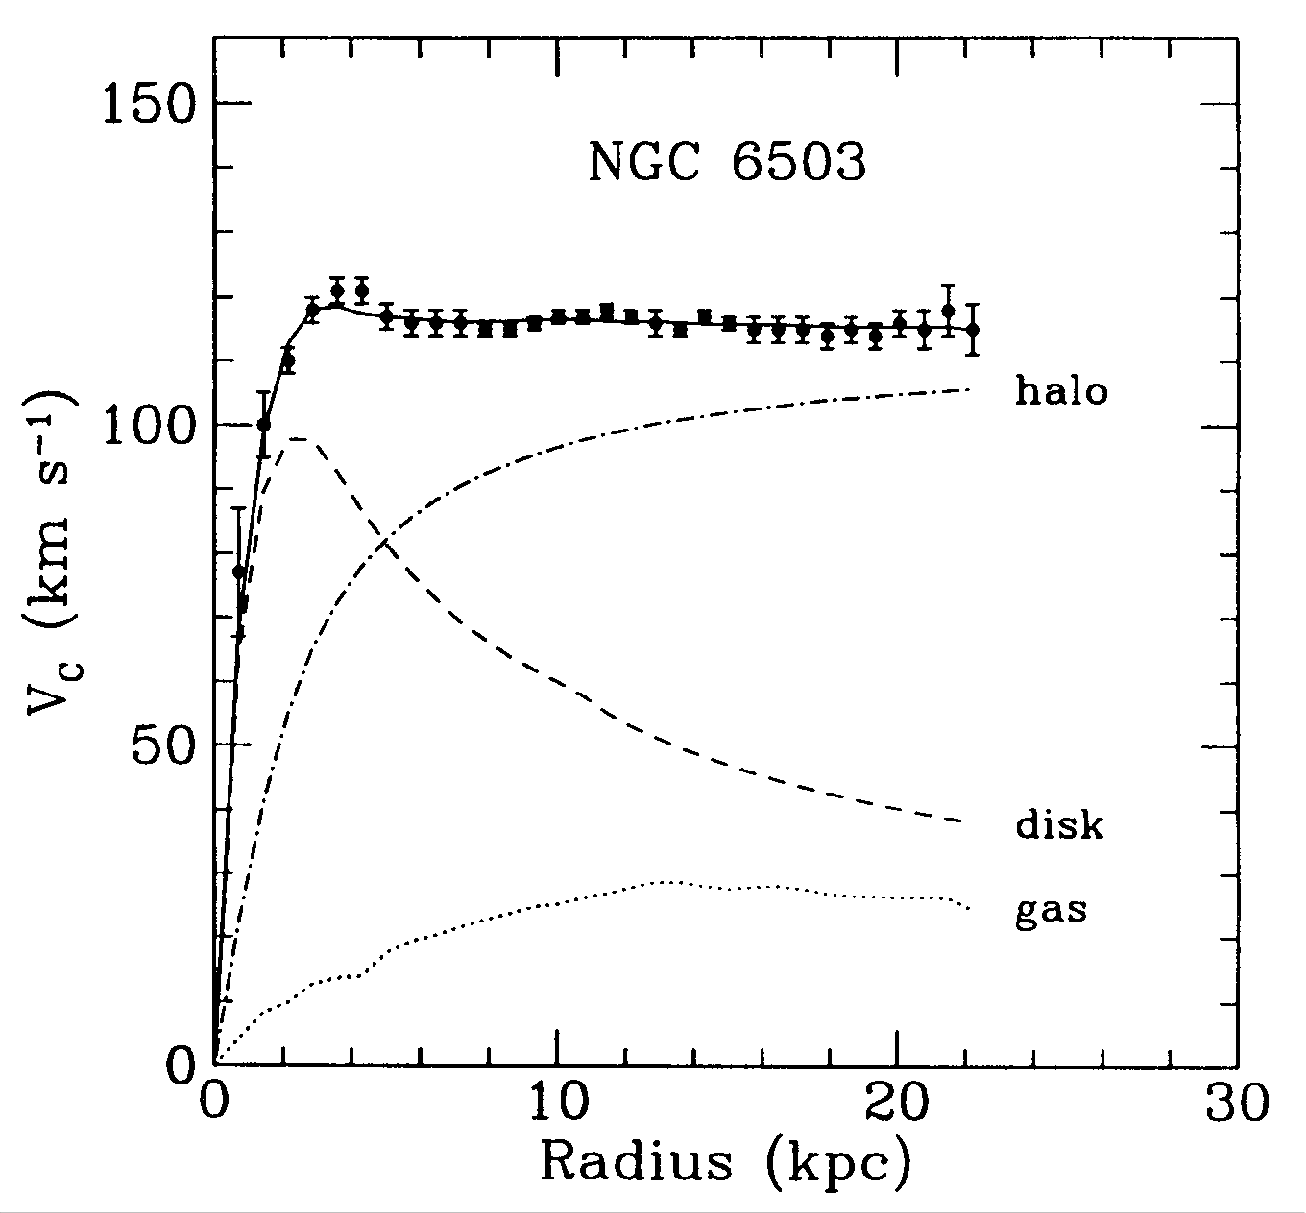
\includegraphics[width=\largefigwidth]{plots/theory/rotationcurve.png}}

  \subfloat[]{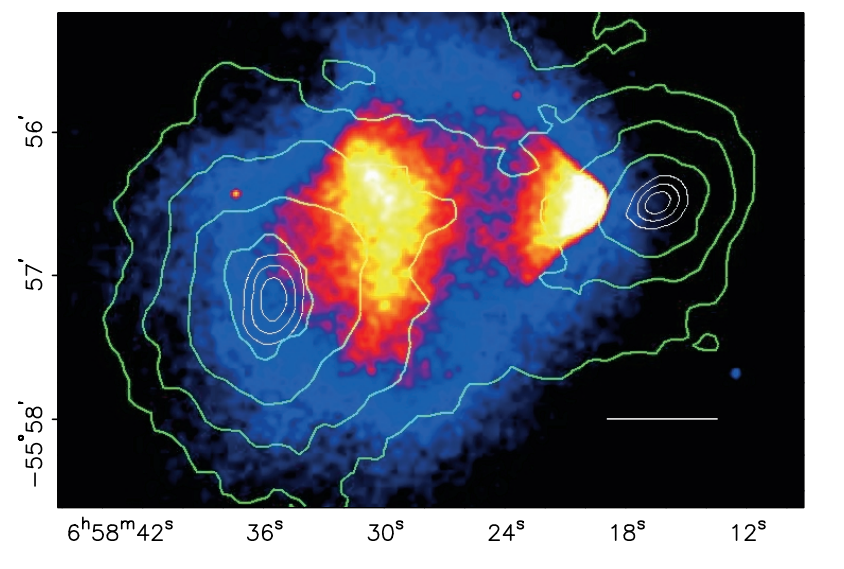
\includegraphics[width=\largefigwidth]{plots/theory/bulletcluster.png}}
  \DIFdelbeginFL %DIFDELCMD < \caption{%%%
\DIFdelendFL \DIFaddbeginFL \caption[Evidence for DM: (a) Rotation velocity in the galaxy NGC 6503 as a function of distance from the galactic centre. (b) The disk and gas components shown are made of visible matter, while the halo component shows the effect of adding an additional DM halo to the galaxy. A superposition of X-ray (colour-scale) and gravitational lensing (green contours) images of the bullet cluster of galaxies.]{\DIFaddendFL Evidence for \DIFdelbeginFL %DIFDELCMD < \ac{DM}%%%
\DIFdelendFL \DIFaddbeginFL \DIFaddFL{DM}\DIFaddendFL : (a) Rotation velocity in the galaxy NGC 6503 as a function of distance from the galactic centre~\cite{Freese:2008cz}. (b) The disk and gas components shown are made of visible matter, while the halo component shows the effect of adding an additional \DIFdelbeginFL %DIFDELCMD < \ac{DM} %%%
\DIFdelendFL \DIFaddbeginFL \DIFaddFL{DM }\DIFaddendFL halo to the galaxy. A superposition of X-ray (colour-scale) and gravitational lensing (green contours) images of the bullet cluster of galaxies~\cite{1538-4357-648-2-L109}.}
  \label{fig:dmevidence}
\end{figure}

\section{Searching for dark matter with Higgs bosons}
\label{sec:higgsdm}
%mention collider searches for Dark matter use MET and need associated production
A \ac{SM} 125 \GeV Higgs boson can only decay to invisible final states by first decaying to a pair of \PZ bosons, which then both decay to neutrinos. The branching fraction for this process is less than 1\%~\cite{Heinemeyer:1559921}, so the observation of larger invisible branching ratios of the Higgs boson, \BRinv, would be strong evidence for new physics and could indicate couplings to \ac{DM}-like particles. Observing decays of Higgs or Higgs-like bosons to \ac{DM} presents an experimental problem in that the final state particles are not visible to the particle detectors used at the Large Hadron Collider (\LHC), such as the Compact Muon Solenoid, CMS~\cite{Chatrchyan:2008aa}, which the data used in this thesis were collected with. Therefore, if a Higgs boson were to be created alone and decay to \ac{DM} there would be no way to observe these decays. Fortunately, several Higgs boson production mechanisms (as described in \SectionRef{sec:higprod} below), lead to additional particles being created with the Higgs boson. By conservation of momentum, the vectorial sum of the momenta of these additional particles transverse to the \LHC beams will be non-zero due to the unobserved particles. This missing transverse momentum, \MET, can therefore be used to identify the presence of \ac{DM} particles in the event. This type of search is referred to as a direct search.

%indirect searches and current Higgs properties limits
Another indication of Higgs boson decays to unseen particles would be a difference between the total decay width of the Higgs boson and the sum of the decay widths of all visible decays. This type of search is referred to as an indirect search. For both direct and indirect searches it is necessary to understand how the Higgs boson is produced and how it decays.

\subsection{Higgs boson production and decay at the LHC}
\label{sec:higprod}
%Detail Higgs production and decays in order to motivate searching for invisible decays in the VBF channel
The LHC (discussed in detail in \SectionRef{sec:lhc}) collides protons at high energies. The results of these collisions are referred to as ``events''. The dominant production mechanisms for Higgs bosons in high energy proton collisions are shown in \FigureRef{fig:smprodfeyn}, and they have the cross-sections shown in \FigureRef{fig:smprod}. It can be seen that \ac{ggH} production, where two gluons fuse via a quark loop to produce a Higgs boson (as shown in \FigureRef{fig:smprodfeyn}a), has the highest cross-section across the full Higgs boson mass range shown. Unfortunately, this production mode normally results in no visible particles in the final state and therefore most \ac{ggH} events cannot be used to search for invisibly decaying Higgs bosons. In some \ac{ggH} events there is \ac{QCD} radiation from the initial state particles (\ac{ISR}). Due to asymptotic freedom ~\cite{PhysRevLett.30.1343,PhysRevLett.30.1346} these radiated quarks and gluons each result in a collimated ``jet'' of hadrons in the final state, and thus allow invisibly decaying Higgs boson searches to be performed. However, the visible particles in these events are hard to distinguish from other similar \ac{QCD} background processes with much larger cross-sections, so \ac{ggH} is not the most promising channel for invisibly decaying Higgs boson searches.

The next highest production cross-section is that for \ac{VBF}. As can be seen in \FigureRef{fig:smprodfeyn}b, this process involves two incoming quarks both radiating vector bosons which fuse, resulting in a Higgs boson. The two initial quarks form jets in the final state, providing visible particles with which to perform an invisibly decaying Higgs boson search. Furthermore, the lack of a strong force connection (referred to as ``colour connection'') between the two quarks means that the resulting jets have a distinctive topology, being well separated in their angle to the beamline, and also that there is very little other hadronic activity in \ac{VBF} events. This distinctive topology and high cross-section make \ac{VBF} the most sensitive production channel for invisibly decaying Higgs boson searches. For this reason, this thesis will focus on the \ac{VBF} channel.

After \ac{VBF}, \ac{VH} production has the next highest cross-section. \ac{VH} results in a Higgs boson and a vector boson, which decays resulting in visible particles in the final state allowing invisibly decaying Higgs boson searches to be carried out. In the case of leptonic vector boson decays, these final state particles can be relatively easy to identify, resulting in lower backgrounds than in the case of searches in the \ac{VBF} and \ac{ggH} channels. However, the lower cross-section means that the \ac{VH} channel is not as sensitive as \ac{VBF}.

Finally, the fourth highest cross-section Higgs boson production channel is top quark associated production, where the final state consists of two top quarks and a Higgs boson. Whilst the top quarks do decay to visible particles which could be identified, the cross-section for this process is too low, and the backgrounds are too high for an invisibly decaying Higgs boson search to be carried out using the Run 1 \LHC data.

\begin{figure}
    %ggh
  \subfloat[]{
    \begin{fmfgraph*}(150,150)
      \fmfleft{i0,i2,ix,i3,i5}
      \fmfright{o0,o3,o1,o4,o6}
      \fmf{phantom,tension=4/3}{i2,v1,o3}
      \fmf{phantom,tension=4/3}{i3,v2,o4}
      \fmffreeze
      \fmf{gluon,tension=4/3}{i2,v1}
      \fmf{gluon,tension=4/3}{i3,v2}
      \fmf{fermion,tension=0}{v1,v2}
      \fmf{fermion,tension=2/3}{v2,v3,v1}
      \fmf{dashes}{v3,o1}
      \fmflabel{$g$}{i2}
      \fmflabel{$g$}{i3}
      \fmflabel{$H$}{o1}
  \end{fmfgraph*}}    
  %vbf
  \hspace{3.5cm}
  \subfloat[]{
    \begin{fmfgraph*}(150,150)
      \fmfleft{i1,i2}
      \fmfright{o1,o2,o3}
      \fmf{fermion}{i1,v1,o1}
      \fmf{fermion}{i2,v2,o3}
      \fmf{photon,label=$W,,Z$}{v1,v3}
      \fmf{photon,label=$W,,Z$}{v2,v3}
      \fmf{dashes}{v3,o2}
      \fmflabel{$q$}{i1}
      \fmflabel{$q$}{i2}
      \fmflabel{$q$}{o1}
      \fmflabel{$q$}{o3}
      \fmflabel{$H$}{o2}
  \end{fmfgraph*}
  \vspace{.5cm}
}

  \vspace{.5cm}

    %Higgstrahlung
  \subfloat[]{
    \begin{fmfgraph*}(150,150)
      \fmfleft{i1,i2}
      \fmfright{o1,o2}
      \fmf{fermion}{i1,v1}
      \fmf{fermion}{v1,i2}
      \fmf{photon,label=$W,,Z$}{v1,v2}
      \fmf{photon}{v2,o1}
      \fmf{dashes}{v2,o2}
      \fmflabel{$q$}{i1}
      \fmflabel{$\bar{q}$}{i2}
      \fmflabel{$W,Z$}{o1}
      \fmflabel{$H$}{o2}
  \end{fmfgraph*}
  \vspace{.5cm}
}
  \hspace{3.5cm}
  %tth
  \subfloat[]{
    \begin{fmfgraph*}(150,150)
      \fmfleft{i0,i1,i4,i5,i6,i2,i3}
      \fmfright{o0,o1,o2,o3,o4}
      \fmf{gluon,tension=3/2}{i1,v1}
      \fmf{gluon,tension=3/2}{i2,v2}
      \fmf{fermion}{o1,v1,v3,v2,o3}
      \fmf{dashes,tension=3/2}{v3,o2}
      \fmflabel{$g$}{i1}
      \fmflabel{$g$}{i2}
      \fmflabel{$\bar{t}$}{o1}
      \fmflabel{$t$}{o3}
      \fmflabel{$H$}{o2}
  \end{fmfgraph*}
}

  \caption{Feynman diagrams for the four \DIFdelbeginFL %DIFDELCMD < \ac{SM} %%%
\DIFdelendFL \DIFaddbeginFL \DIFaddFL{SM }\DIFaddendFL Higgs boson production processes with the highest cross-sections: \DIFdelbeginFL %DIFDELCMD < \ac{ggH} %%%
\DIFdelendFL \DIFaddbeginFL \DIFaddFL{ggH }\DIFaddendFL (a), \DIFdelbeginFL %DIFDELCMD < \ac{VBF} %%%
\DIFdelendFL \DIFaddbeginFL \DIFaddFL{VBF }\DIFaddendFL (b), \DIFdelbeginFL %DIFDELCMD < \ac{VH} %%%
\DIFdelendFL \DIFaddbeginFL \DIFaddFL{VH }\DIFaddendFL (c) and top quark associated production (d).}
  \label{fig:smprodfeyn}
\end{figure}

\begin{figure}
  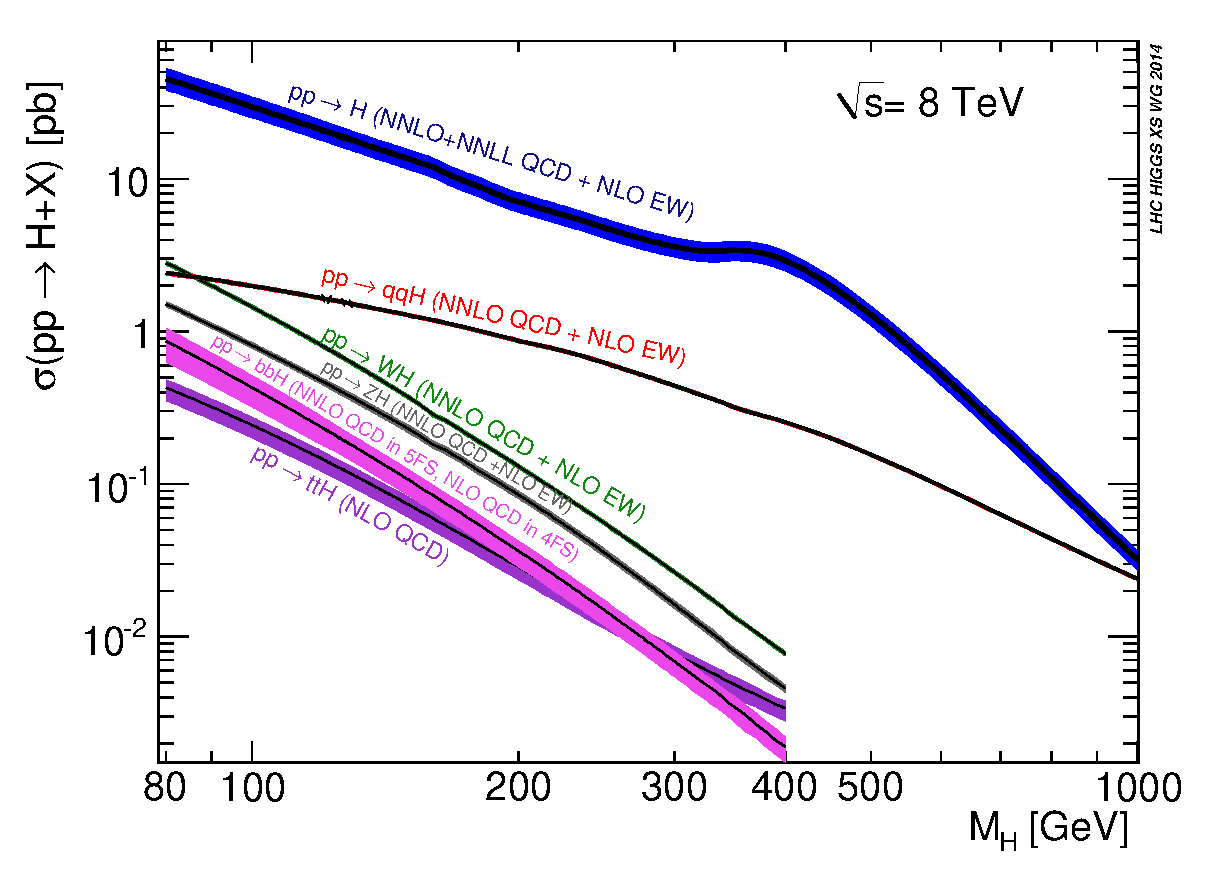
\includegraphics[width=\largefigwidth]{plots/theory/XS_8TeV.eps}
  \DIFdelbeginFL %DIFDELCMD < \caption{%%%
\DIFdelendFL \DIFaddbeginFL \caption[Cross-sections for Higgs boson production via the most common production processes at $\sqrt{s}=8 \TeV$ as a function of Higgs boson mass, $m_{H}$. The widths of the lines represent the theoretical uncertainties on the cross-section calculation.]{\DIFaddendFL Cross-sections for Higgs boson production via the most common production processes at $\sqrt{s}=8 \TeV$ as a function of Higgs boson mass, $m_{H}$~\cite{Heinemeyer:1559921}. The widths of the lines represent the theoretical uncertainties on the cross-section calculation.}
  \label{fig:smprod}
\end{figure}

%talk about SM decays and what SM invisible branching fraction is, direct vs indirect
As mentioned in the introduction to this section, limits can be placed on the Higgs boson's coupling to invisible particles by comparing the total decay width of the Higgs boson to the sum of the decay widths for all the visible Higgs boson final states. The branching ratio for the dominant Higgs boson decays as a function of the mass of the Higgs boson can be seen in \FigureRef{fig:smdecay}a. Because a particle's coupling to the Higgs boson is proportional to its mass, the heavier particles have larger branching ratios, with the caveat that particles above half the mass of the Higgs boson, have reduced couplings due to their being created virtually. The \ac{SM} total width of the Higgs boson is shown in \FigureRef{fig:smdecay}b. For a 125 \GeV Higgs boson, the width is only a few \MeV, which is below the current resolution with which it can be measured~\cite{Khachatryan201464}.
Therefore, in order to use the total visible decay width to constrain \BRinv an assumption about the total decay width must be made. 

The current measurements of the branching ratios of the Higgs boson to the 5 most frequent final states can be seen in \FigureRef{fig:smdecaymeasurement}a. The log-likelihood as a function of \BRinv, obtained from these measured branching ratios, assuming the \ac{SM} total Higgs boson decay width, is shown in \FigureRef{fig:smdecaymeasurement}b. It can be seen that whilst the most likely value is approximately zero, values of \BRinv up to $\sim35\%$ are not excluded at the 95\% \ac{CL}. This limit leaves significant parameter space open for \ac{BSM} Higgs boson decays. As the above limit assumes the \ac{SM} Higgs boson total width, it is possible that the branching ratio to invisible final states is much larger, making the case for direct measurements even more compelling. Additional Higgs-like bosons that decay to invisible final states are also not excluded.


\begin{figure}
  \subfloat{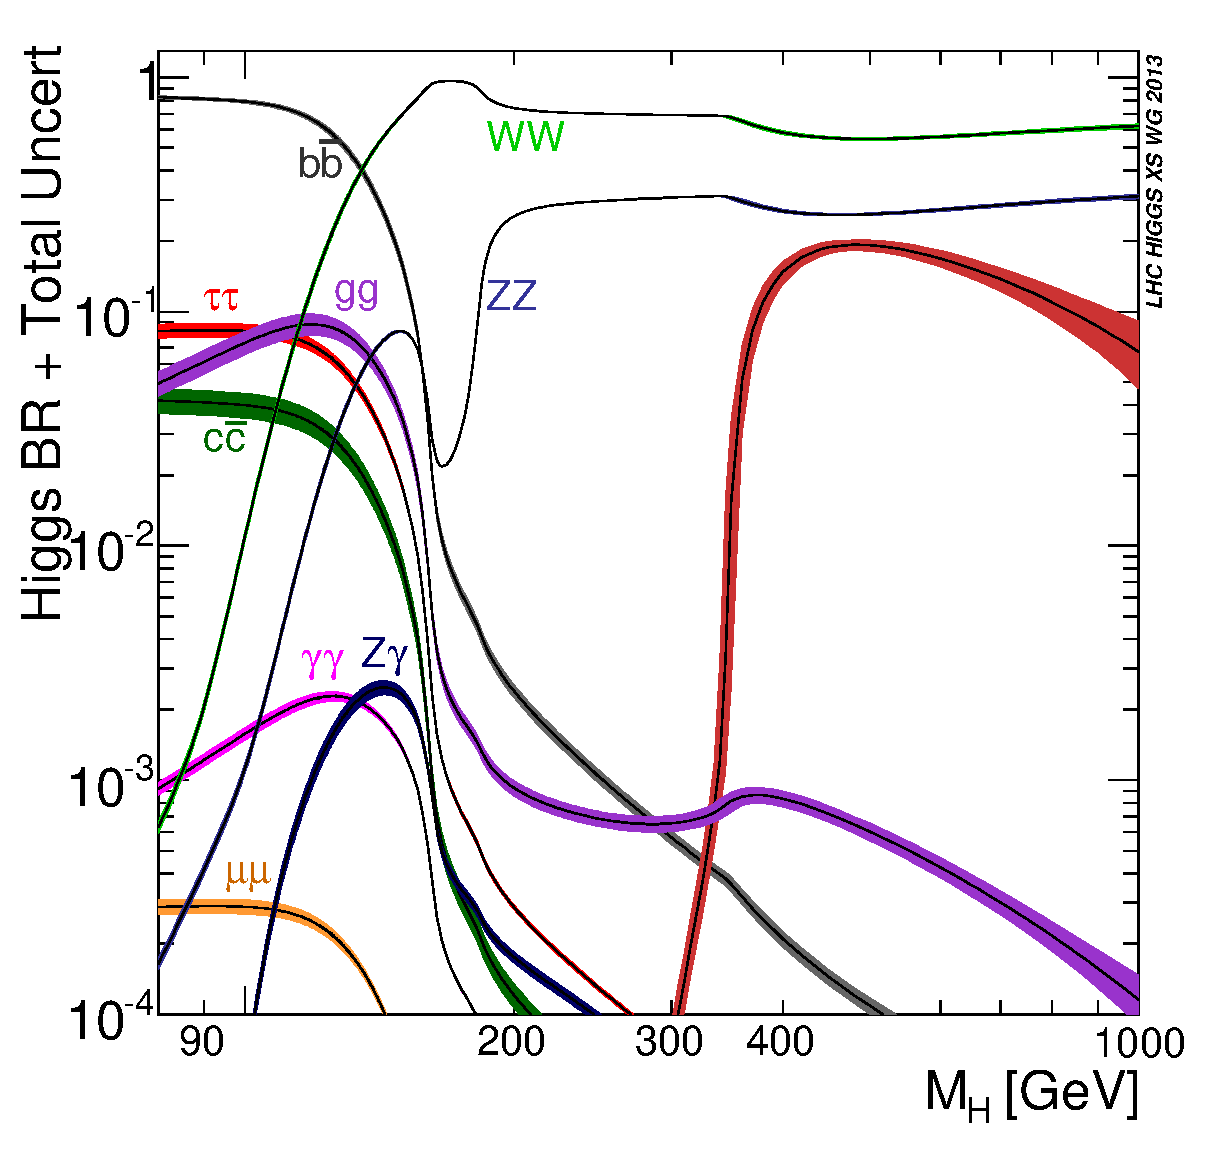
\includegraphics[width=.65\largefigwidth]{plots/theory/Higgs_BR.eps}}
  \subfloat{\includegraphics[width=.65\largefigwidth]{plots/theory/SM_Width-eps-converted-to.pdf}}
  \DIFdelbeginFL %DIFDELCMD < \caption{%%%
\DIFdelendFL \DIFaddbeginFL \caption[Branching ratios for the dominant Higgs boson decays as a function of Higgs boson mass with the line widths representing the uncertainties (a), and the SM Higgs boson total width, $\Gamma_{H}$, as a function of Higgs boson mass (b).]{\DIFaddendFL Branching ratios for the dominant Higgs boson decays as a function of Higgs boson mass with the line widths representing the uncertainties (a), and the \DIFdelbeginFL %DIFDELCMD < \ac{SM} %%%
\DIFdelendFL \DIFaddbeginFL \DIFaddFL{SM }\DIFaddendFL Higgs boson total width, $\Gamma_{H}$, as a function of Higgs boson mass (b)~\cite{Heinemeyer:1559921}.}
  \label{fig:smdecay}
\end{figure}

\begin{figure}
  \subfloat[]{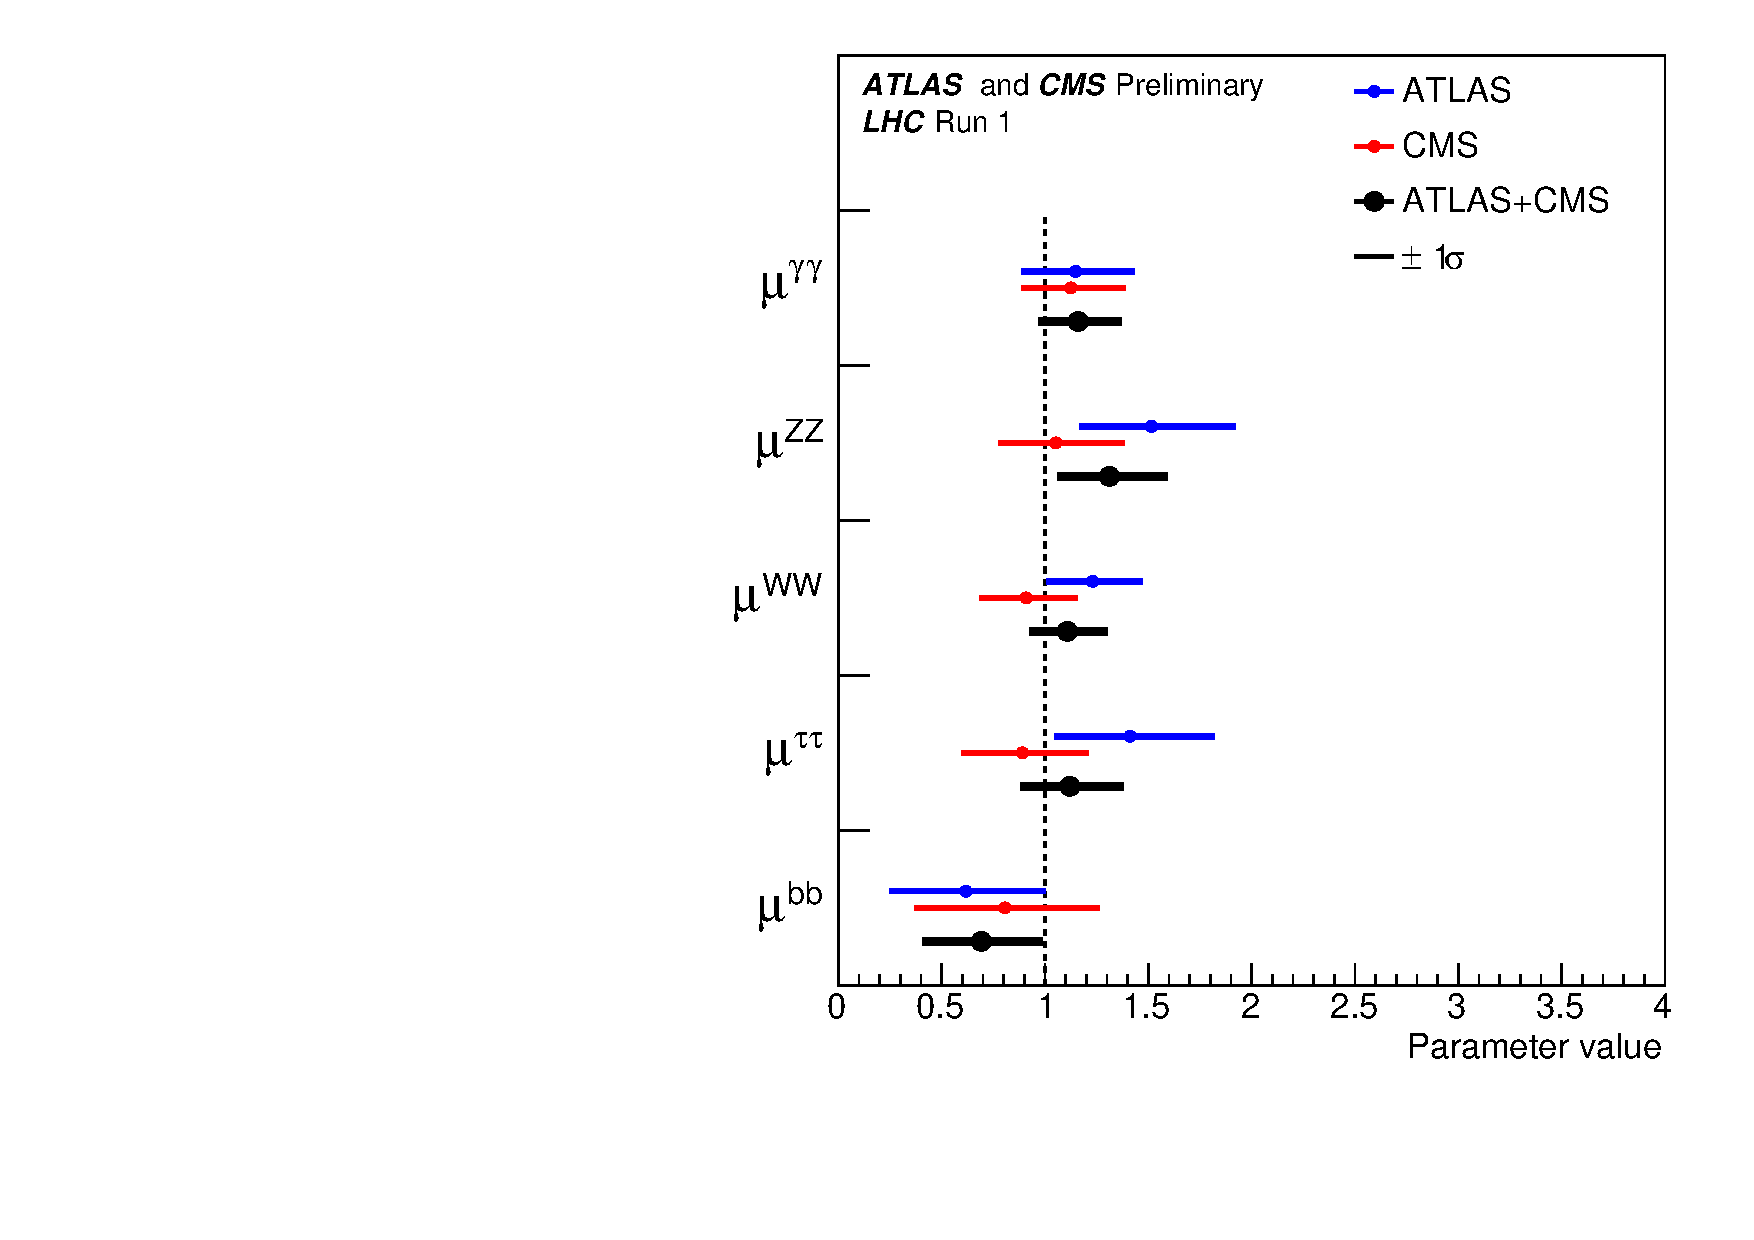
\includegraphics[width=.65\largefigwidth]{plots/theory/smdecaybrlimits.pdf}}
  \subfloat[]{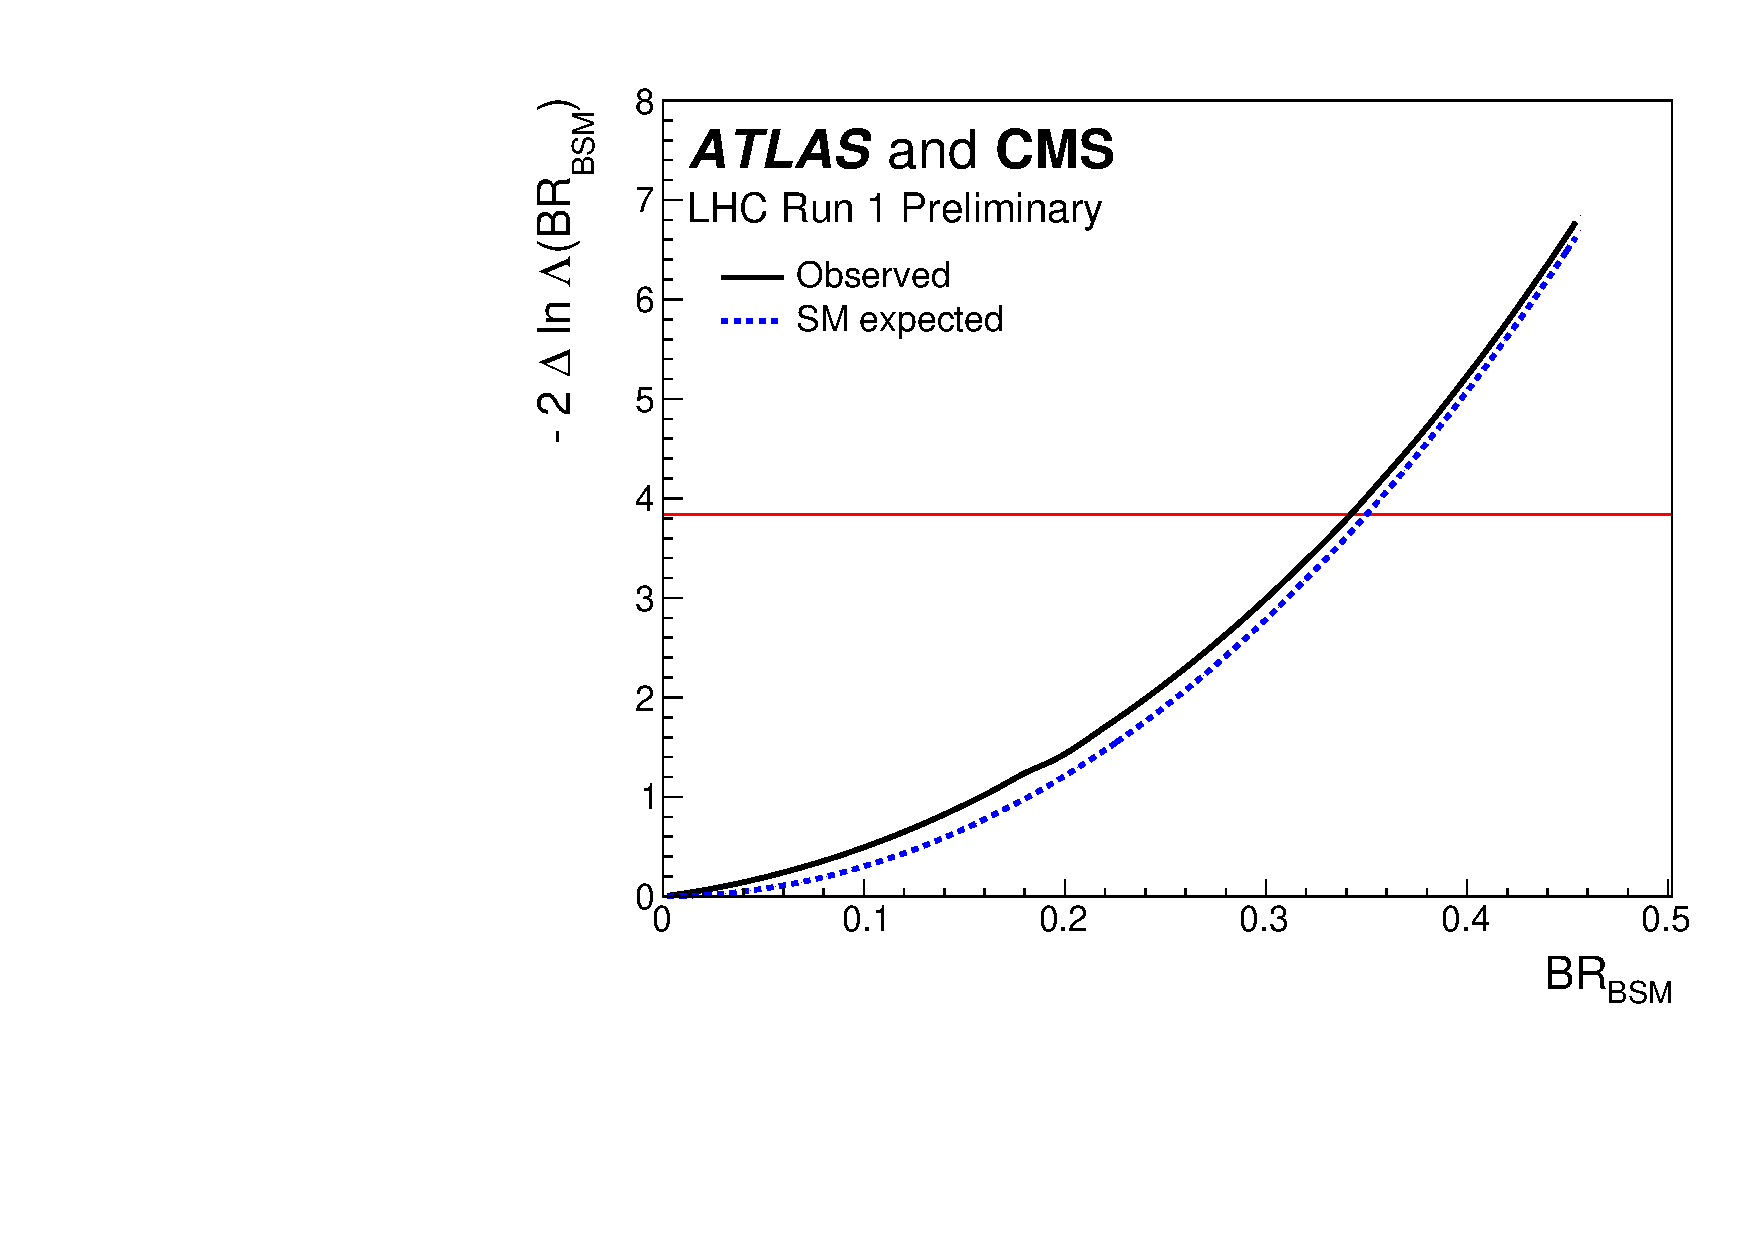
\includegraphics[width=.65\largefigwidth]{plots/theory/smbrbsmlikelihood.pdf}}
  \DIFdelbeginFL %DIFDELCMD < \caption{%%%
\DIFdelendFL \DIFaddbeginFL \caption[Best fit results for the decay signal strengths of the five highest branching ratio Higgs boson decays from a combination of CMS and ATLAS Run 1 data (a). The negative log-likelihood as a function of \BRinv, here denoted $\rm{BR_{BSM}}$ (b).]{\DIFaddendFL Best fit results for the decay signal strengths of the five highest branching ratio Higgs boson decays from a combination of CMS and ATLAS~\cite{Aad:1129811} Run 1 data (a). The negative log-likelihood as a function of \BRinv, here denoted $\rm{BR_{BSM}}$ (b)~\cite{CMS-PAS-HIG-15-002}.}
  \label{fig:smdecaymeasurement}
\end{figure}

\subsection{Some extensions of the standard model incorporating dark matter}
\label{sec:DMextensions}
%Introduce theories that are used for pheno work
Whilst current evidence for \ac{DM} is gravitational, the majority of extensions to the \ac{SM} which include \ac{DM} also require other interactions of the proposed \ac{DM} particles \DIFdelbegin \DIFdel{. }\DIFdelend \DIFaddbegin \DIFadd{to explain the similarity between the amounts of each present in the universe. Through these interactions the equilibrium between the annihilation of }\ac{DM} \DIFadd{to visible matter and vice versa in the early universe naturally leads to similar amounts of each being present. However, without some coupling between the two types of matter there is no a priori reason for their energy densities to be even of the same order of magnitude. 
}

 \DIFaddend These interactions then allow the particle the \ac{DM} interacts with to act as a ``mediator'' between the \ac{SM} and \ac{DM} particles, for example as in \FigureRef{fig:simplifiedmodelfeynmandiag}a. As all known particles with mass interact with the Higgs boson, it might be expected that \ac{DM}'s interactions with the \ac{SM} are mediated by the Higgs boson or a Higgs-like particle.

\begin{figure}
  \subfloat[]{
    \begin{fmfgraph*}(150,150)
      \fmfleft{i1,i2}
      \fmfright{o1,o4,o2,o5,o3}
      \fmf{fermion}{i1,v1,o1}
      \fmf{fermion}{i2,v2,o3}
      \fmf{photon,label=$W,,Z$,label.side=left}{v1,v3}
      \fmf{photon,label=$W,,Z$,label.side=right}{v2,v3}
      \fmf{dashes,label=$H/A$}{v3,v4}
      \fmf{fermion}{v4,o4}
      \fmf{fermion}{v4,o5}
      \fmflabel{$q$}{i1}
      \fmflabel{$q$}{i2}
      \fmflabel{$q$}{o1}
      \fmflabel{$q$}{o3}
      \fmflabel{$\chi$}{o4}
      \fmflabel{$\chi$}{o5}
  \end{fmfgraph*}
  \vspace{.5cm}
}
  \subfloat[]{
    \begin{fmfgraph*}(150,150)
      \fmfleft{i1,i2}
      \fmfright{o1,o4,o2,o5,o3}
      \fmf{fermion}{i1,v1,o1}
      \fmf{fermion}{i2,v2,o3}
      \fmf{gluon}{v1,v3}
      \fmf{gluon}{v2,v3}
      \fmfdot{v3}
      \fmf{dashes,label=$H/A$}{v3,v4}
      \fmf{fermion}{v4,o4}
      \fmf{fermion}{v4,o5}
      \fmflabel{$q$}{i1}
      \fmflabel{$q$}{i2}
      \fmflabel{$q$}{o1}
      \fmflabel{$q$}{o3}
      \fmflabel{$\chi$}{o4}
      \fmflabel{$\chi$}{o5}
  \end{fmfgraph*}
  \vspace{.5cm}
}
%\vspace{.5cm}
  \subfloat[]{
    \begin{fmfgraph*}(150,150)
      \fmfleft{i1,i2}
      \fmfright{o1,o4,o2,o5,o3}
      \fmf{fermion}{i1,v1,o1}
      \fmf{fermion}{i2,v2,o3}
      \fmf{photon,label=$W,,Z$,label.side=left}{v1,v4}
      \fmf{photon,label=$W,,Z$,label.side=right}{v2,v4}
      \fmfdot{v4}
      \fmf{fermion}{v4,o4}
      \fmf{fermion}{v4,o5}
      \fmflabel{$q$}{i1}
      \fmflabel{$q$}{i2}
      \fmflabel{$q$}{o1}
      \fmflabel{$q$}{o3}
      \fmflabel{$\chi$}{o4}
      \fmflabel{$\chi$}{o5}
  \end{fmfgraph*}
  \vspace{.5cm}
}
  \caption{Feynman diagrams for the \DIFdelbeginFL \DIFdelFL{dark matter }\DIFdelendFL \DIFaddbeginFL \DIFaddFL{DM }\DIFaddendFL theories considered. (a) \ac{VBF} production of a scalar, $H$, or pseudoscalar $A$ mediator. (b) Gluon based production of an $H$ or $A$ mediator. (c) An effective field theory where the mediator has been replaced by a contact interaction between the vector bosons and a hypothetical \DIFdelbeginFL %DIFDELCMD < \ac{DM} %%%
\DIFdelendFL \DIFaddbeginFL \DIFaddFL{DM }\DIFaddendFL particle.}
  \label{fig:simplifiedmodelfeynmandiag}
\end{figure}

%efts
In \ChapterRef{chap:interp} two classes of these \ac{DM} interaction models are investigated. The first class is \ac{EFT} type models. In these models the mediator is assumed to be much heavier than the momentum transferred through it. This high mass allows the behaviour of the mediator to be replaced by a contact interaction between the \ac{SM} and \ac{DM} particles as shown in \FigureRef{fig:simplifiedmodelfeynmandiag}c. Following the notation in \ReferenceRef{PhysRevD.88.116009}, the particular contact interaction operators considered in this thesis, which each represent a different Lorentz structure for the contact interaction, are:
\begin{align}
  \mathcal{L}_{\rm{D5a}} &=\frac{1}{\Lambda} \left[\bar{\chi}\chi\right] \left[\frac{\PZ_{\mu}\PZ^{\mu}}{2}+\PW_{\mu}^{+}\PW^{-\mu}\right],\\
  \mathcal{L}_{\rm{D5b}} &=\frac{1}{\Lambda} \left[\bar{\chi}\gamma^{5}\chi\right] \left[\frac{\PZ_{\mu}\PZ^{\mu}}{2}+\PW_{\mu}^{+}\PW^{-\mu}\right],\\
  \mathcal{L}_{\rm{D5c}} &=\frac{g_{2}}{\Lambda} \left[\bar{\chi}\sigma^{\mu\nu}\chi\right]\left[\frac{\partial_{\mu}\PZ_{\nu}-\partial_{\nu}\PZ_{\mu}}{cos\theta_{W}} - ig_{2} \left(\PW^{+}_{\mu}W^{-}_{\nu} - \PW^{+}_{\nu}W^{-}_{\mu}\right)\right],\\
  \mathcal{L}_{\rm{D5d}} &=\frac{g_{2}}{\Lambda} \left[\bar{\chi}\sigma_{\mu\nu}\chi\right] \epsilon^{\mu\nu\rho\sigma}\left[\frac{\partial_{\sigma}\PZ_{\rho}-\partial_{\rho}\PZ_{\sigma}}{cos\theta_{W}} - ig_{2} \left(\PW^{+}_{\sigma}W^{-}_{\rho} - \PW^{+}_{\rho}W^{-}_{\sigma}\right)\right],\\
  \mathcal{L}_{\rm{D6a}} &=\frac{g_{2}}{\Lambda^{2}}\partial^{\nu} \left[\bar{\chi}\gamma^{\mu}\chi\right] \left[\frac{\partial_{\mu}\PZ_{\nu}-\partial_{\nu}\PZ_{\mu}}{cos\theta_{W}} - ig_{2} \left(\PW^{+}_{\mu}W^{-}_{\nu} - \PW^{+}_{\nu}W^{-}_{\mu}\right)\right],\\
  \mathcal{L}_{\rm{D6b}} &=\frac{g_{2}}{\Lambda^{2}}\partial_{\nu} \left[\bar{\chi}\gamma_{\mu}\chi\right] \epsilon^{\mu\nu\rho\sigma}\left[\frac{\partial_{\sigma}\PZ_{\rho}-\partial_{\rho}\PZ_{\sigma}}{cos\theta_{W}} - ig_{2} \left(\PW^{+}_{\sigma}W^{-}_{\rho} - \PW^{+}_{\rho}W^{-}_{\sigma}\right)\right],\\
  \mathcal{L}_{\rm{D7a}} &=\frac{1}{\Lambda^{3}} \left[\bar{\chi}\chi\right] \PW^{i,\mu\nu}\PW_{\mu\nu}^{i},\\
  \mathcal{L}_{\rm{D7b}} &=\frac{1}{\Lambda^{3}} \left[\bar{\chi}\gamma^{5}\chi\right] \PW^{i,\mu\nu}\PW_{\mu\nu}^{i},\\
  \mathcal{L}_{\rm{D7c}} &=\frac{1}{\Lambda^{3}} \left[\bar{\chi}\chi\right] \epsilon^{\mu\nu\rho\sigma} \PW^{i}_{\mu\nu}\PW_{\rho\sigma}^{i},\\
  \mathcal{L}_{\rm{D7d}} &=\frac{1}{\Lambda^{3}} \left[\bar{\chi}\gamma^{5}\chi\right] \epsilon^{\mu\nu\rho\sigma} \PW^{i}_{\mu\nu}\PW_{\rho\sigma}^{i},\\
\end{align}
where the \ac{DM} particles, $\chi$, are assumed to be electromagnetically and colour neutral Dirac fermions, and $\PW^{i,\mu\nu}$ is the field strength tensor for the unbroken \DIFdelbegin \DIFdel{$SU\left(2\right)_{L}$ }\DIFdelend \DIFaddbegin \DIFadd{$SU\!\left(2\right)_{L}$ }\DIFaddend gauge bosons. $\Lambda$ is the ``scale'' of the interaction, which is a combination of the mass of the replaced mediator, $M$, and its couplings to both \ac{DM} and the \ac{SM}, $g$, such that $\Lambda\sim M/g^{2}$. Whilst the \ac{EFT} models have the advantage of being simple to interpret, having only one parameter, the validity of the assumption that the momentum transferred through the interaction is much smaller than the mass of the mediator must be checked carefully, especially where the couplings between the mediator and the \ac{DM} are expected to be small. As well as direct searches for invisibly decaying Higgs bosons, several other experimental techniques, including direct \DIFdelbegin \DIFdel{dark matter }\DIFdelend \DIFaddbegin \ac{DM} \DIFaddend detection are able to set constraints on these models~\cite{ourdmpaper}.%advantages and disadvantages of efts. 

The second class of models are so-called simplified models. In these models an explicit choice of mediator is made, removing the need to make an assumption about the transferred momentum. The specific mediators considered are the 125 \GeV Higgs boson, and scalar and pseudoscalar mediators with heavier masses.

In the case of the 125 \GeV Higgs boson mediator, the following term is added to the Lagrangian:
\begin{equation}
  \mathcal{L}_{H\chi\chi}=-g_{\chi}\left(\bar{\chi}\chi\right)H,
\end{equation}
where the \ac{DM} particles, $\chi$, are again assumed to be Dirac fermions, and $g_{\chi}$ is the Higgs boson coupling to \ac{DM}. As the mediator is very similar to the \ac{SM} Higgs boson all the production mechanisms described in \SectionRef{sec:higprod} are possible, with the most sensitive being \ac{VBF}. If the \DIFdelbegin \DIFdel{dark matter }\DIFdelend \DIFaddbegin \ac{DM} \DIFaddend mass is below 62.5 \GeV, i.e. it can be created via a real mediator, this interaction leads to an increased invisible decay width of the Higgs boson:
\begin{equation}
  \label{eq:offshellsmhiggs}
  \Gamma\left(H\rightarrow\bar{\chi}\chi\right)=\frac{g_{\chi}^{2}m_{H}}{8\pi}\left(1-\frac{4m_{\chi}^{2}}{m_{H}^{2}}\right),
\end{equation}
where $m_{H}$ and $m_{\chi}$ are the masses of the Higgs boson and the \DIFdelbegin \DIFdel{dark matter }\DIFdelend \DIFaddbegin \ac{DM} \DIFaddend particle respectively~\cite{ourdmpaper}. For heavier \ac{DM} masses, off-shell production, i.e. through a virtual mediator, is still possible, however there is no invisible branching fraction of the Higgs boson.

For the heavier scalar and pseudoscalar mediators, as well as the free term for the mediator, the terms added to the Lagrangian for the scalar, $H$, and the pseudoscalar, $A$, are:
\begin{align}
  \mathcal{L}_{H}&=-g_{\chi}H\bar{\chi}\chi-\sum_{f}\frac{g_{\rm{V}}y_{f}}{\sqrt{2}}H\bar{f}f\\
  \mathcal{L}_{A}&=-ig_{\chi}A\bar{\chi}\gamma^{5}\chi-\sum_{f}\frac{ig_{\rm{V}}y_{f}}{\sqrt{2}}A\bar{f}\gamma^{5}f,\\
\end{align}
respectively, where $g_{\rm{V}}$ is the coupling of the mediator to visible particles, $f$ are the \ac{SM} fermions, and $y_{f}$ are the \ac{SM} fermion Yukawa couplings~\cite{PhysRevD.91.015017}. The couplings to the \ac{SM} fermions are chosen to be proportional to the \ac{SM} Yukawa couplings so as to avoid constraints from measurements of flavour physics observables~\cite{D'Ambrosio2002155}. Due to the measured couplings of the vector bosons to the 125 \GeV Higgs boson being compatible with the \ac{SM}, the \DIFdelbegin \DIFdel{new mediators do not interact with vector bosons }\DIFdelend \DIFaddbegin \DIFadd{coupling between the new mediators and the vector bosons must be small}\DIFaddend ~\cite{CMS-PAS-HIG-15-002}. \DIFaddbegin \DIFadd{For the models considered here the coupling is taken to be zero. }\DIFaddend This lack of vector boson couplings makes \ac{VBF} production, as in \FigureRef{fig:simplifiedmodelfeynmandiag}a, not possible, and leads to the most common production channel for \DIFdelbegin \DIFdel{dark matter }\DIFdelend \DIFaddbegin \ac{DM} \DIFaddend in association with two jets being the fusion of two gluons as shown in \FigureRef{fig:simplifiedmodelfeynmandiag}b. This gluon fusion occurs, like that seen in the production of the \ac{SM} Higgs boson, through a fermion loop, which is dominated by the top quark due to it having the largest Yukawa coupling.

Again, when the \DIFdelbegin \DIFdel{dark matter }\DIFdelend \DIFaddbegin \ac{DM} \DIFaddend is less than half the mass of the mediator the mediator will have a non-zero invisible branching ratio. The \DIFdelbegin \DIFdel{dark matter }\DIFdelend \DIFaddbegin \ac{DM} \DIFaddend production rate will be given by this branching ratio multiplied by the production rate of the mediator. For mediator masses below twice the top quark's mass, and \DIFdelbegin \DIFdel{dark matter }\DIFdelend \DIFaddbegin \ac{DM} \DIFaddend masses much higher than the $b$ quark's mass, this branching ratio is approximately 100\%. The \DIFdelbegin \DIFdel{dark matter }\DIFdelend \DIFaddbegin \ac{DM} \DIFaddend production rate is therefore, under the assumption that $g_{V}=g_{\chi}$, proportional to $g_{\chi}^{2}$. For mediator masses larger than twice the top quark's mass, assuming $g_{V}=g_{\chi}$, the branching ratio becomes approximately 40\%~\cite{ourdmpaper} and the production rate remains proportional to $g_{\chi}^{2}$. For \DIFdelbegin \DIFdel{dark matter }\DIFdelend \DIFaddbegin \ac{DM} \DIFaddend produced through an off-shell mediator the \DIFdelbegin \DIFdel{dark matter }\DIFdelend \DIFaddbegin \ac{DM} \DIFaddend production rate becomes proportional to $g_{v}^{2}g_{\chi}^{2}$, which simplifies to $g_{\chi}^{4}$ under the assumption of equal \ac{DM} and visible couplings.


\section{Simulation}
\label{sec:sim}
The simulation of \LHC proton-proton collisions can be factorised into several distinct stages, as shown in \FigureRef{fig:factorisation}. The first stage is the hard-scattering of two incoming elements of the proton, called ``partons''. The momentum of each of these partons is sampled from a \ac{PDF}. These \ac{PDF}s give the probability for each incoming parton type to have a certain fraction of the proton's energy at the given hard-scatter energy scale, sometimes referred to as the \ac{QCD} scale. Due to the high energy nature of the hard-scatter, perturbation theory at fixed order can be used for both \ac{QCD} and electroweak interactions at this stage of the simulation. Quantities calculated using the particles which result from the hard-scattering are referred to as ``parton level''.

After the hard-scatter the resulting particles undergo ``parton showering'', which is an iterative process of repeated \ac{QCD} radiation until the particles reach an energy where perturbation theory is no longer valid. After parton showering, particles undergo hadronisation, where colourless hadrons are formed, and allowed to decay. The results of this hadronisation and decay process are four-momentum vectors for each particle which are referred to as the ``generator-level'' particles. In most cases the generator level particles are then processed by a \textsc{Geant}~\cite{Agostinelli2003250} 4 based simulation of the CMS detector. For the work described in \ChapterRef{chap:interp} a \textsc{Delphes}~\cite{Favereau2014} based simulation of the CMS detector \DIFdelbegin \DIFdel{, which }\DIFdelend \DIFaddbegin \DIFadd{was used. This simulation }\DIFaddend is only approximate, but greatly decreases the computational power needed to process the same number of events.

Several \ac{MC} generators are used to carry out the perturbative hard-scattering calculations. Some, such as \textsc{Pythia}~\cite{Sjöstrand2008852}, are also able to provide the hard-scatter calculation for a wide ranges of processes as well as perform other stages of the factorisation. Others like \textsc{MadGraph}~\cite{Alwall2014} and \textsc{Powheg}~\cite{Nason:2004rx,Frixione:2007vw,Alioli:2010xd} only calculate the hard-scattering component. However, these other generators produce more accurate results for certain processes they have been tuned to, or allow for a larger range of processes to be simulated than the multipurpose generators such as \textsc{Pythia}. In all of the \ac{MC} samples used in this thesis, the results of the hard-scatter are then passed on to \textsc{Pythia} for parton showering and hadronisation.

Finally, some generators, such as MCFM~\cite{PhysRevD.68.094021}, VBFNLO~\cite{Baglio:2014uba,Arnold:2011wj,Arnold20091661}, \textsc{Top++} ~\cite{Czakon20142930} and \textsc{FEWZ}~\cite{PhysRevD.86.094034} are used only to calculate cross-sections very accurately at \ac{NLO} or \ac{NNLO}. These calculations are much more computationally intensive than the lower order calculations above, which renders them unsuitable for generating full \ac{MC} samples with a four vector for each final state particle.

\begin{figure}
  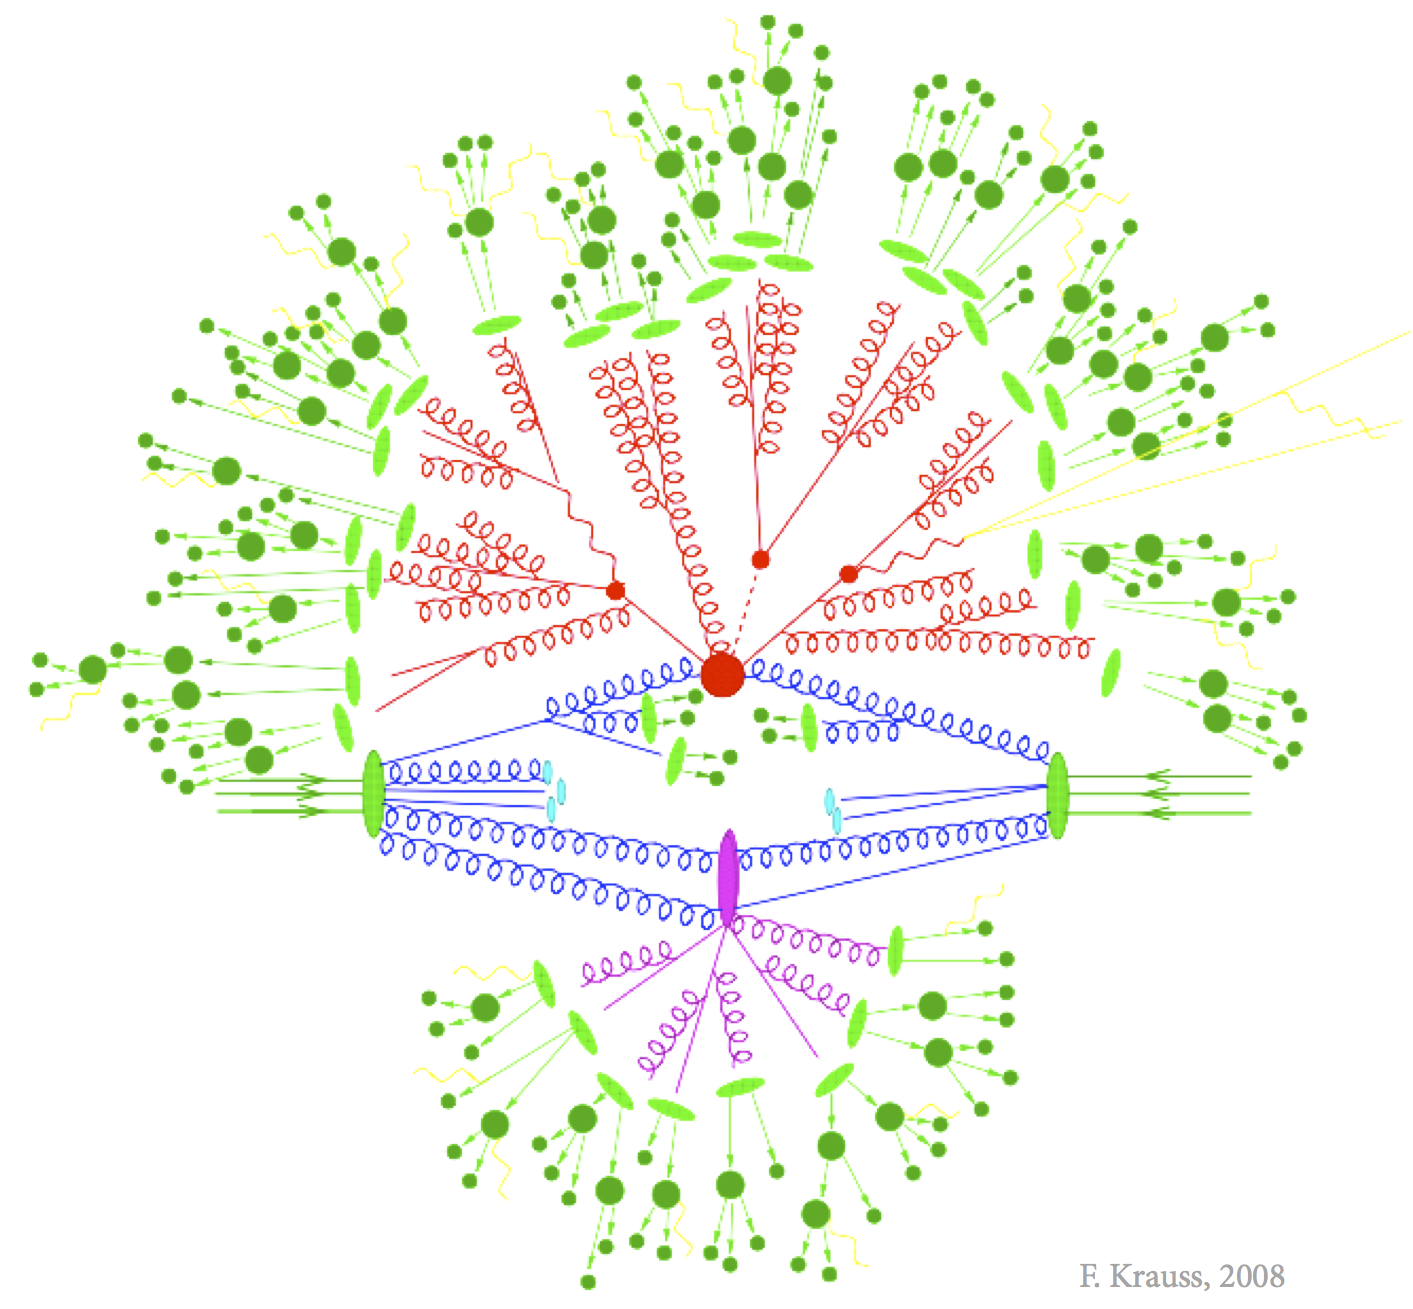
\includegraphics[width=\largefigwidth]{plots/theory/factorisation.png}
  \DIFdelbeginFL %DIFDELCMD < \caption{%%%
\DIFdelendFL \DIFaddbeginFL \caption[A schematic diagram of the factorised components of the simulation of proton-proton collisions. First the hard-scatter of two of the incoming partons (shown in blue) is simulated at the centre of the event. The results of this scatter then undergo parton showering (shown in red), followed by hadronisation (shown in green) when the energy of the quarks and gluons is low enough that bound states can be formed.]{\DIFaddendFL A schematic diagram of the factorised components of the simulation of proton-proton collisions. First the hard-scatter of two of the incoming partons (shown in blue) is simulated at the centre of the event. The results of this scatter then undergo parton showering (shown in red), followed by hadronisation (shown in green) when the energy of the quarks and gluons is low enough that bound states can be formed~\cite{krauss-diag}.}
  \label{fig:factorisation}
\end{figure}

\section{Statistics of exclusion limits}
\label{sec:stats}
%introduce cls and limit setting
Limits on the parameters of theoretical models are presented throughout this thesis. These limits are set by performing a hypothesis test to discriminate between a null, \DIFdelbegin \DIFdel{background only }\DIFdelend \DIFaddbegin \DIFadd{background-only }\DIFaddend model, hypothesis, $b$\DIFaddbegin \DIFadd{, }\DIFaddend and a test hypothesis, the signal process, $s$, plus background model. The particular procedure used is based on the CL$_{S}$ statistic\DIFaddbegin \DIFadd{~\mbox{%DIFAUXCMD
\cite{Read:2002hq}
}%DIFAUXCMD
}\DIFaddend and was developed by the LHC Higgs Combination Group~\cite{ATL-PHYS-PUB-2011-011}.  This procedure is used by both the ATLAS~\cite{Aad:1129811} and CMS experiments.

The procedure starts by defining a likelihood function, $\mathcal{L}$, which quantifies how likely a certain observation is given the expectation under a given hypothesis. $\mathcal{L}$ takes the form:
\begin{equation}
  \label{eq:likelihood}
  \mathcal{L}=\displaystyle\prod_{i}Poisson\left(n_{i}|\nu_{i}\left(\mu,\theta\right)\right)\cdot\prod_{j}Constraint\left(\theta_{j},\bar{\theta}\right),
\end{equation}
where the first term is the contribution from the Poisson probability to observe $n_{i}$ events in each analysis category, $i$, given a predicted number of events from the hypothesis, $\nu_{i}$. $\nu_{i}$ is a function of a signal strength parameter, $\mu$, which in the case of the signal hypothesis being an SM Higgs boson is 1 for the SM and 0 for the \DIFdelbegin \DIFdel{background only }\DIFdelend \DIFaddbegin \DIFadd{background-only }\DIFaddend case, and the ``nuisance \DIFdelbegin \DIFdel{paramters}\DIFdelend \DIFaddbegin \DIFadd{parameters}\DIFaddend ,'' $\theta$, which account for the uncertainties on parameters of the signal and background models and any correlations between them. The second term in \EquationRef{eq:likelihood} represents the constraints on the allowed values of these nuisance parameters, with $\bar{\theta}$ being the best estimate of $\theta$ obtained from external measurements. The shape of the constraint function varies depending on the nuisance parameter it represents. For example, uncertainties on the event yield in a category are usually modelled with log-normal constraints, which exclude negative values of the event yield. 

Profile likelihood ratios, q$_{\mu}$, are then calculated, which are defined as:
\begin{equation}
  \label{eq:proflikelihood}
  q_{\mu} = -2 \ln\frac{\mathcal{L}(obs|\mu \cdot s + b,\hat{\theta}_{\mu})}{\mathcal{L}(obs|\hat{\mu} \cdot s + b,\hat{\theta})}\,,
\end{equation}
where $obs$ is the observation, and $\hat{\mu}$ and $\hat{\theta}$ are the values of $\theta$ and $\mu$ where the likelihood is maximised given the constraint $0 \geqslant \hat{\mu} \geqslant \mu$. $\hat{\theta}_{\mu}$ are the values of the nuisance parameters that maximise the likelihood for a given $\mu$. The profile likelihood ratio therefore describes how likely it is to observe a signal strength equal to or higher than $\mu$ compared to the most likely signal strength.

The CL$_{s}$ statistic itself is then defined as:
\begin{equation}
  \label{eq:cls}
  CL_{s} = \frac{P(q_{\mu}\geqslant q_{\mu}^{obs} | \mu \cdot s + b)}{P(q_{\mu}\geqslant q_{\mu}^{obs}|b)}\,,
\end{equation}
where \DIFdelbegin \DIFdel{the }\DIFdelend \DIFaddbegin \DIFadd{$q_{\mu}^{obs}$ is the observed profile likelihood ratio and the }\DIFaddend probability $P$ of a given $q_{\mu}$ can be calculated using the asymptotic limit approximation~\cite{Cowan:2010js}. The region in which a signal strength $\mu \cdot s$ is excluded at the $1 - \alpha$ \ac{CL} is then the region for which CL$_{s}$ is less than or equal to $\alpha$, i.e. when the signal hypothesis is $\alpha$ times less probable than the background.
\chapter{The \LHC and the \CMS experiment}
\label{chap:detector}
This chapter introduces the \CMS experiment and the \LHC~\cite{1748-0221-3-08-S08001}. In \SectionRef{sec:lhc} an overview of the \LHC and the chain of accelerators which feed into it is given. This is then followed in \SectionRef{sec:CMSInDetail} by a description of the \CMS experiment focusing on the aspects most relevant to the search for invisibly decaying Higgs bosons.

\section{The \LHC}
\label{sec:lhc}
The \LHC is situated \DIFdelbegin \DIFdel{100m }\DIFdelend \DIFaddbegin \DIFadd{100}\,\DIFadd{m }\DIFaddend underground in a tunnel formerly built for the LEP accelerator~\cite{lepdesign} at CERN near Geneva, Switzerland. It is a \DIFdelbegin \DIFdel{27km }\DIFdelend \DIFaddbegin \DIFadd{27}\,\DIFadd{km }\DIFaddend storage ring which accelerates both protons and heavy ions and collides them at the highest centre-of-mass energies of any collider built to date. The work contained in this thesis uses data from proton-proton collisions. These protons are obtained by taking hydrogen gas and stripping its atoms of their electrons with an electric field. The first accelerator in the chain of accelerators feeding into the \LHC, Linac 2, accelerates the protons to 50\DIFaddbegin \,\DIFaddend \MeV. The protons are then accelerated to 1.4\DIFaddbegin \,\DIFaddend \GeV~by the next accelerator, the \ac{PSB}, which is followed by the \ac{PS} where they reach 25\DIFaddbegin \,\DIFaddend \GeV. The beam energy is then increased to 450\DIFaddbegin \,\DIFaddend \GeV~in the \ac{SPS}. Finally, the protons are injected into the \LHC where, at \DIFaddbegin \DIFadd{the }\DIFaddend time of writing, the maximum energy the beams have been accelerated to is 6.5\DIFaddbegin \,\DIFaddend \TeV, close to the design maximum of 7\DIFaddbegin \,\DIFaddend \TeV.

When \DIFdelbegin \DIFdel{fully }\DIFdelend filled the \LHC contains two counter-rotating beams which are formed of up to 2808 bunches spaced either 25 ns or 50 ns apart and each containing $\mathcal{O}(10^{11})$ protons. The two beams are kept travelling in a \DIFdelbegin \DIFdel{circle }\DIFdelend \DIFaddbegin \DIFadd{closed orbit }\DIFaddend by 1232 superconducting dipole magnets and steered to four collision points around the \LHC. Detectors are situated at these collision points to observe the interactions, the main four being: ALICE~\cite{Aamodt:2008zz}, ATLAS, CMS and LHCb~\cite{Alves:2008zz}. A schematic of the chain of accelerators feeding into the \LHC and the \LHC detectors can be seen in \FigureRef{fig:lhclayout}.

\begin{figure}
  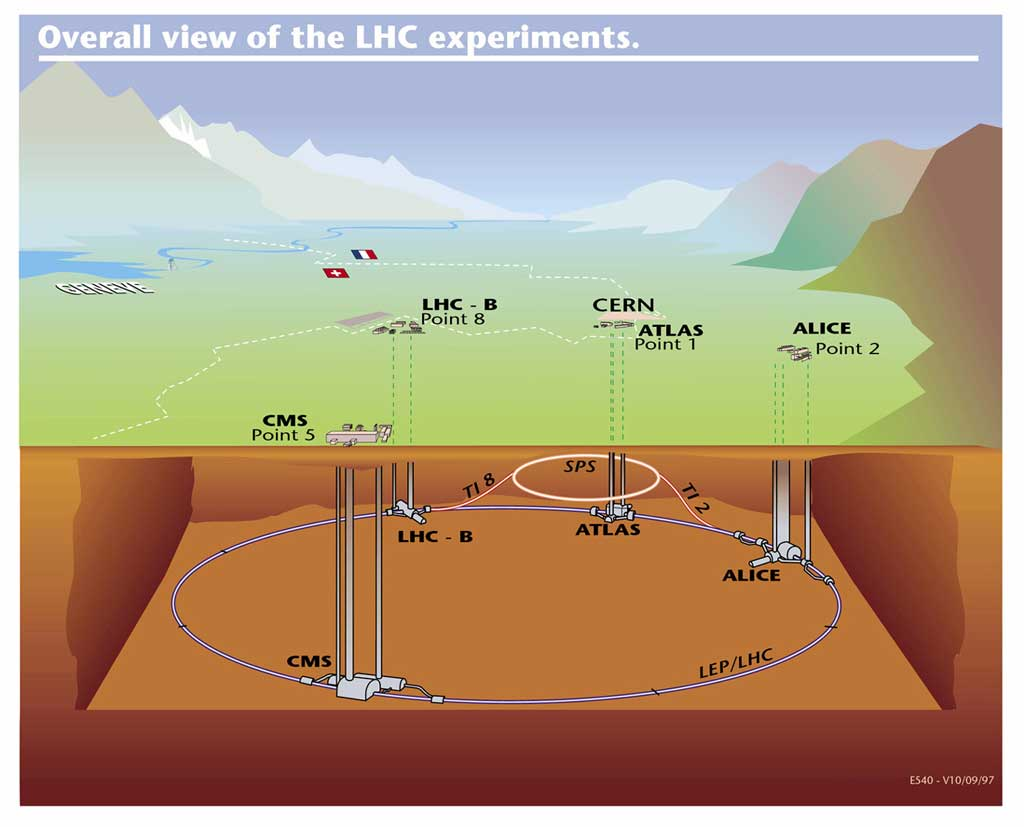
\includegraphics[width=\largefigwidth]{plots/detector/lhc_layout_sch.jpg}
  \DIFdelbeginFL %DIFDELCMD < \caption{%%%
\DIFdelendFL \DIFaddbeginFL \caption[The layout of the chain of accelerators feeding into the \LHC, showing the position of the four main detectors.]{\DIFaddendFL The layout of the chain of accelerators feeding into the \LHC, showing the position of the four main detectors~\cite{lhcexpschematic}.}
  \label{fig:lhclayout}
\end{figure}

When studying a physical process occurring in particle collisions it is important to know how many times it will occur, this can be expressed as:
\begin{equation}
  N = \mathcal{L}\sigma,
\end{equation}
where $\mathcal{L}$, the integrated luminosity, depends only on the parameters of the collisions, and the cross-section, $\sigma$, depends only on the process. In order to observe rare (i.e. low cross-section) processes, such as those studied at the LHC, it is necessary to use very high luminosity datasets. The integrated luminosity is obtained by integrating the instantaneous luminosity over time, so large luminosities can be obtained either by running the accelerator for a long time, or by operating at high instantaneous luminosity. For collisions at the \LHC the instantaneous luminosity is given by:
\begin{equation}
  \mathcal{L}\DIFaddbegin \DIFadd{_{inst}}\DIFaddend =\frac{k_{b}N_{b}^{2}f_{rev}\gamma}{4\pi\epsilon_{n}\beta}\DIFaddbegin \,\DIFaddend \cite{Benedikt:823808},
\end{equation}
where $k_{b}$ is the number of bunches per beam, $N_{b}$ the number of protons per bunch, $f_{rev}$ the revolution frequency, $\epsilon_{n}$ the normalised transverse beam emittance, $\beta^{*}$ the beta-function at the interaction point and $\gamma$ the Lorentz factor. The design instantaneous luminosity of the \LHC is $10^{34}\,\cm^{-2}\rm{s}^{-1}$ with \DIFdelbegin \DIFdel{25ns }\DIFdelend \DIFaddbegin \DIFadd{25 ns }\DIFaddend bunch spacing. The integrated luminosity is defined as \DIFdelbegin \DIFdel{$\mathcal{L}_{int}=\int\mathcal{L}\mathrm{d}t$}\DIFdelend \DIFaddbegin \DIFadd{$\mathcal{L}=\int\mathcal{L}_{inst}\mathrm{d}t$}\DIFaddend .

The \LHC started physics runs in 2010, during which it operated at a centre-of-mass energy of 7\DIFaddbegin \,\DIFaddend \TeV~ and delivered an integrated luminosity of 44.2 \invpb ~to CMS. In 2011 the \LHC also operated at 7\DIFaddbegin \,\DIFaddend \TeV~ and delivered 6.1\DIFaddbegin \,\DIFaddend \invfb to CMS. The centre-of-mass energy was increased to 8\DIFaddbegin \,\DIFaddend \TeV~ in 2012 and 23.3\DIFaddbegin \,\DIFaddend \invfb~of data were delivered to CMS. A summary of the luminosity delivered to CMS during the three periods of Run 1 can be seen in \FigureRef{fig:lumisummary}. In Run 2 the centre-of-mass energy was further increased to 13\DIFaddbegin \,\DIFaddend \TeV~and during 2015 4.09\DIFaddbegin \,\DIFaddend \invfb~of data were delivered to CMS at this energy. In order to be used for physics analysis data must be certified. This certification ensures that the detector was fully operational when the data were recorded. In 2011 5.1\DIFaddbegin \,\DIFaddend \invfb~were certified, in 2012 19.7\DIFaddbegin \,\DIFaddend \invfb~were certified and in 2015 2.2\DIFaddbegin \,\DIFaddend \invfb~were certified.


\begin{figure}
  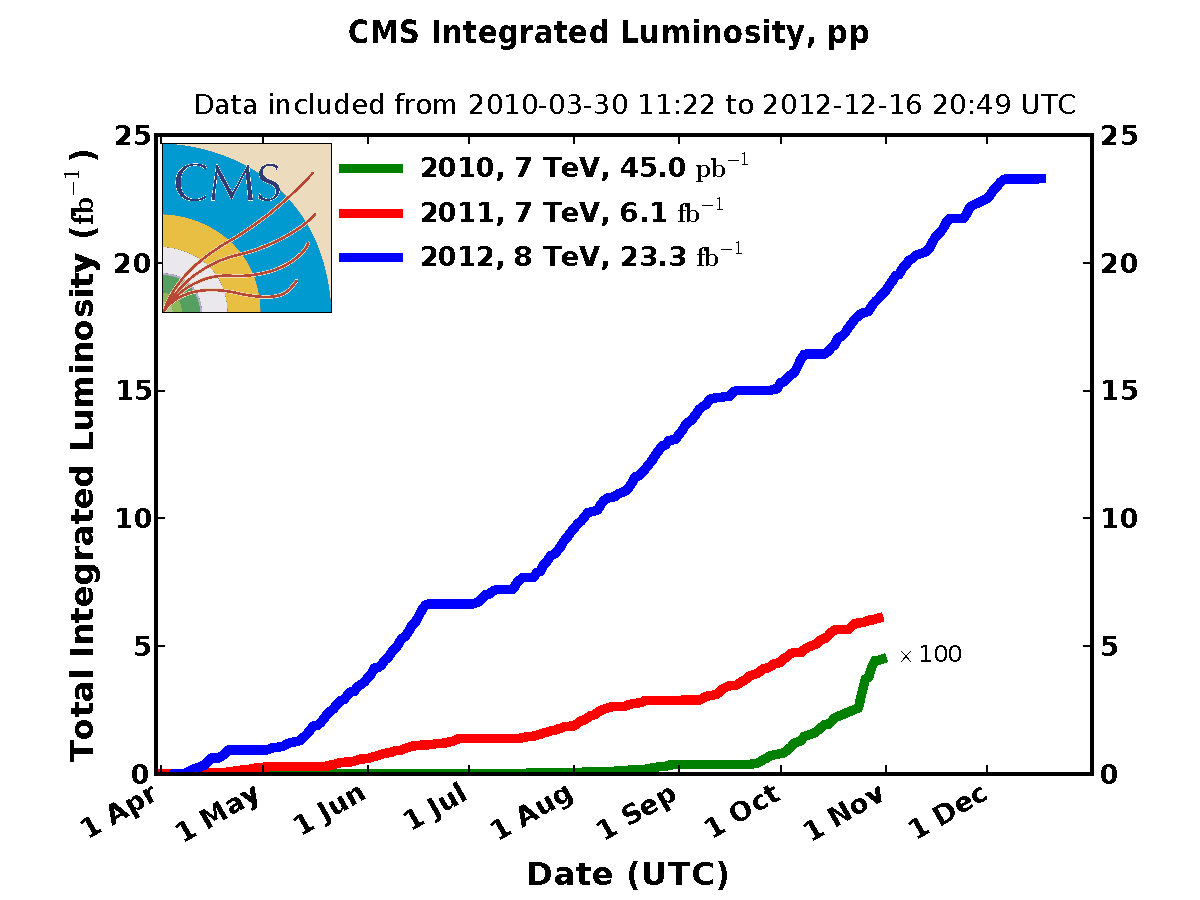
\includegraphics[width=1.2\largefigwidth]{plots/detector/int_lumi_cumulative_pp_2.pdf}
  \DIFdelbeginFL %DIFDELCMD < \caption{%%%
\DIFdelendFL \DIFaddbeginFL \caption[A summary of the luminosity delivered to CMS during Run 1 of the \LHC.]{\DIFaddendFL A summary of the luminosity delivered to CMS during Run 1 of the \LHC \cite{CMSLumiPublic}.}
  \label{fig:lumisummary}
\end{figure}
%??maybe figure for 13 TeV too

The cross-sections for several processes are shown in \FigureRef{fig:xssummary} and it can be seen that the cross-section for VBF Higgs production is approximately 1.5 pb. Therefore, we expect approximately 30000 \DIFdelbegin \DIFdel{VBF produced }\DIFdelend \DIFaddbegin \DIFadd{VBF-produced }\DIFaddend Higgs bosons in the 2012 dataset. By contrast the vector boson production cross-section is approximately 100 nb and the total cross-section for any process is orders of magnitude higher still. The separation of the relatively small number of signal events from the large background is a major challenge for the search for invisibly decaying Higgs bosons.

\begin{figure}
  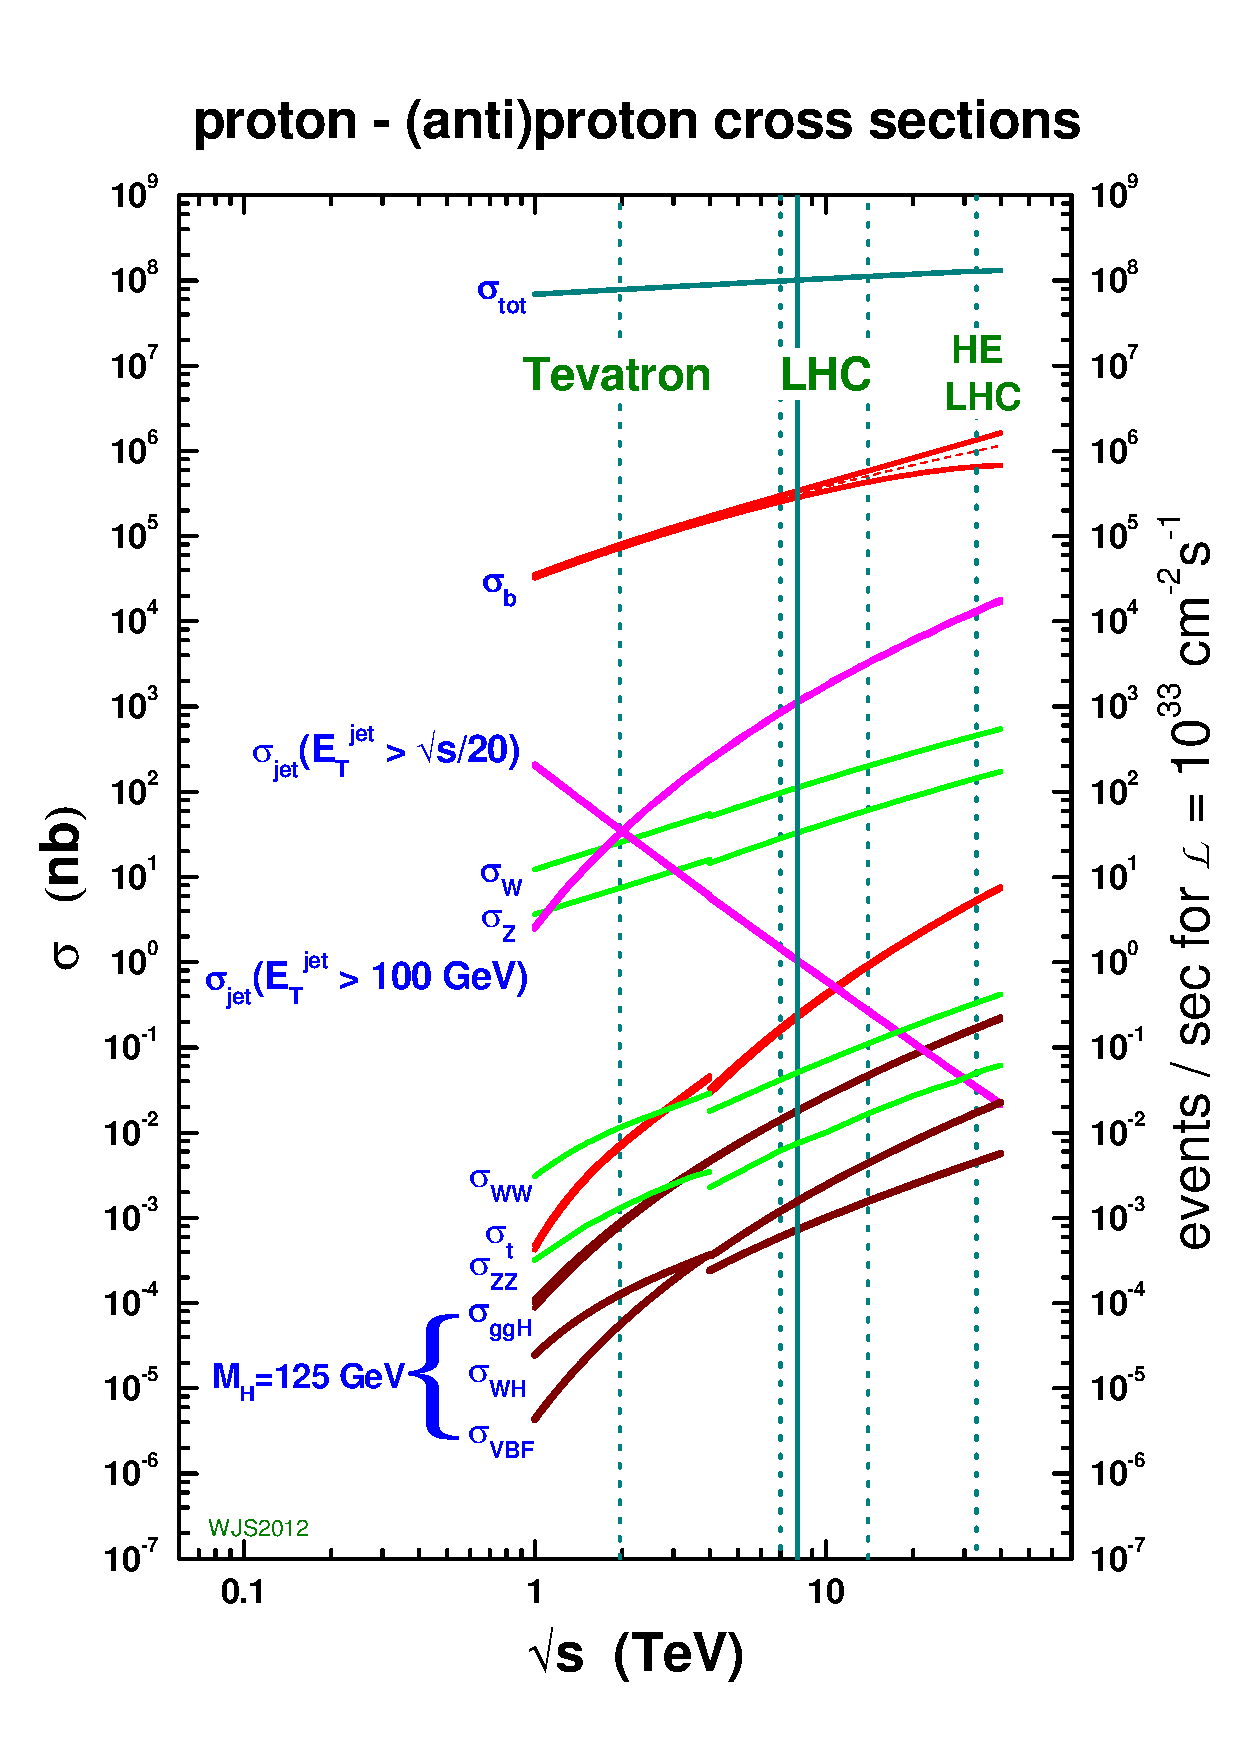
\includegraphics[width=1.2\largefigwidth]{plots/detector/crosssections2012HE_v4.pdf}
  \DIFdelbeginFL %DIFDELCMD < \caption{%%%
\DIFdelendFL \DIFaddbeginFL \caption[Cross-sections for several processes in collisions of protons with protons or anti-protons as a function of centre-of-mass energy. The energies that the \LHC and Tevatron ran at are highlighted.]{\DIFaddendFL Cross-sections for several processes in collisions of protons with protons or anti-protons as a function of centre-of-mass energy. The energies that the \LHC and Tevatron ran at are highlighted\DIFaddbeginFL \DIFaddFL{~}\DIFaddendFL \cite{Stirlingppxs}.}
  \label{fig:xssummary}
\end{figure}

The large total cross-section combined with the high instantaneous luminosities that the \LHC operates at leads to the probability for multiple proton-proton interactions per bunch crossing being high. The distribution of the number of interactions per bunch crossing, $\mu$, can be seen in \FigureRef{fig:pusummary}. The additional interactions on top of the process of interest in a bunch crossing are called \ac{PU}.

\begin{figure}
  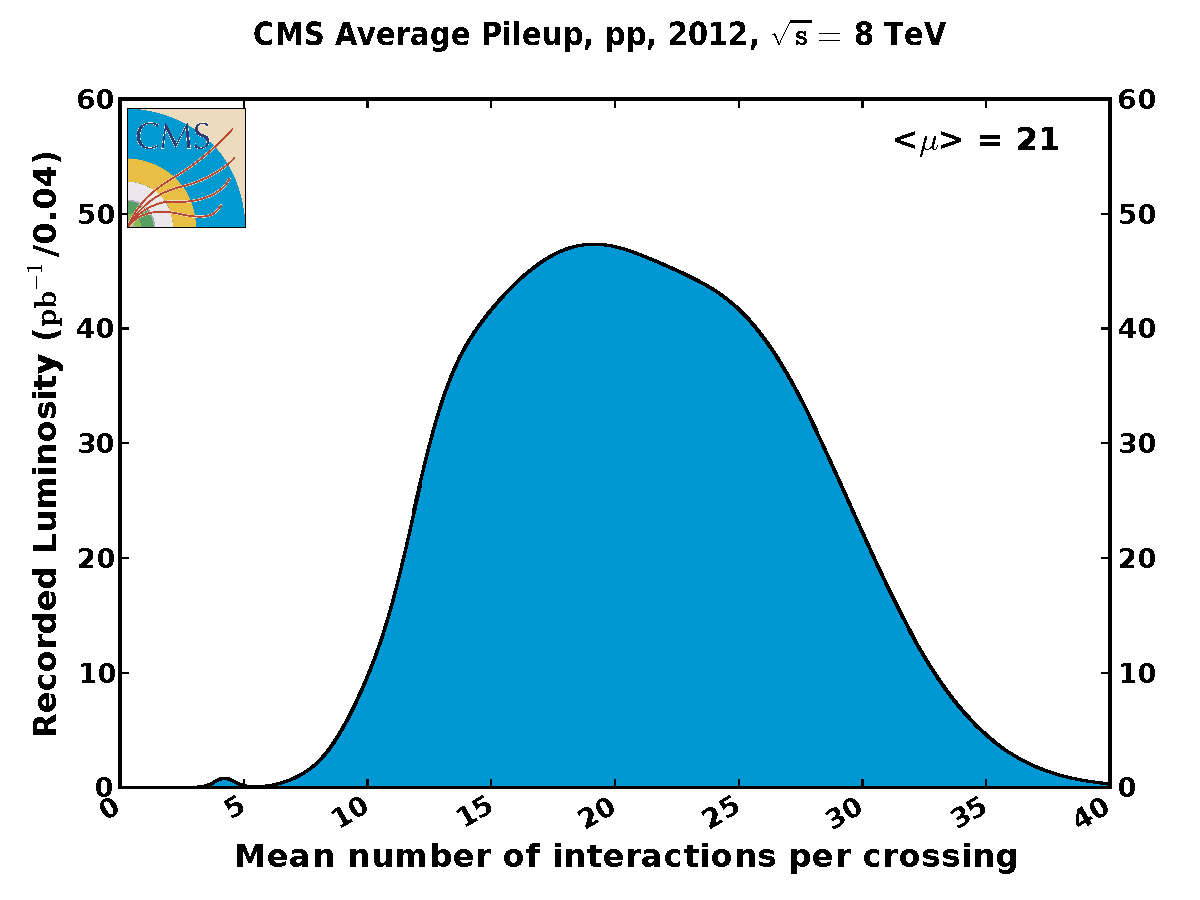
\includegraphics[width=1.2\largefigwidth]{plots/detector/pileup_pp_2012.pdf}
  \DIFdelbeginFL %DIFDELCMD < \caption{%%%
\DIFdelendFL \DIFaddbeginFL \caption[Distribution of the number of interactions per bunch crossing in CMS during 2012 running of the \LHC.]{\DIFaddendFL Distribution of the number of interactions per bunch crossing in CMS during 2012 running of the \LHC \cite{CMSLumiPublic}.}
  \label{fig:pusummary}
\end{figure}


\section{The \CMS experiment}
\label{sec:CMSInDetail}
%Introduction - describe hermetic onion shell concept and introduce subsystems
The CMS detector was designed to search for the SM Higgs and new physics at the TeV energy scale. Both because the nature of new physics is not known and \DIFaddbegin \DIFadd{because }\DIFaddend the SM Higgs has a wide range of decays and production mechanisms CMS must be sensitive to many different types of final state particles and topologies. In order to achieve this it has a hermetic design comprising a barrel, endcaps and a forward calorimetry system. It is composed of several layers of subdetectors each sensitive to different particles as shown in \FigureRef{fig:cmsschematic1}. The hermiticity of the detector is particularly important for the VBF Higgs to invisible search. Further details on the CMS detector beyond those in this section can be found in \ReferenceRef{Chatrchyan:2008aa}. %because, as described in \SectionRef{sec:higprod}, the VBF final state is highly likely to have jets in the forward regions of the detector.

\begin{figure}
  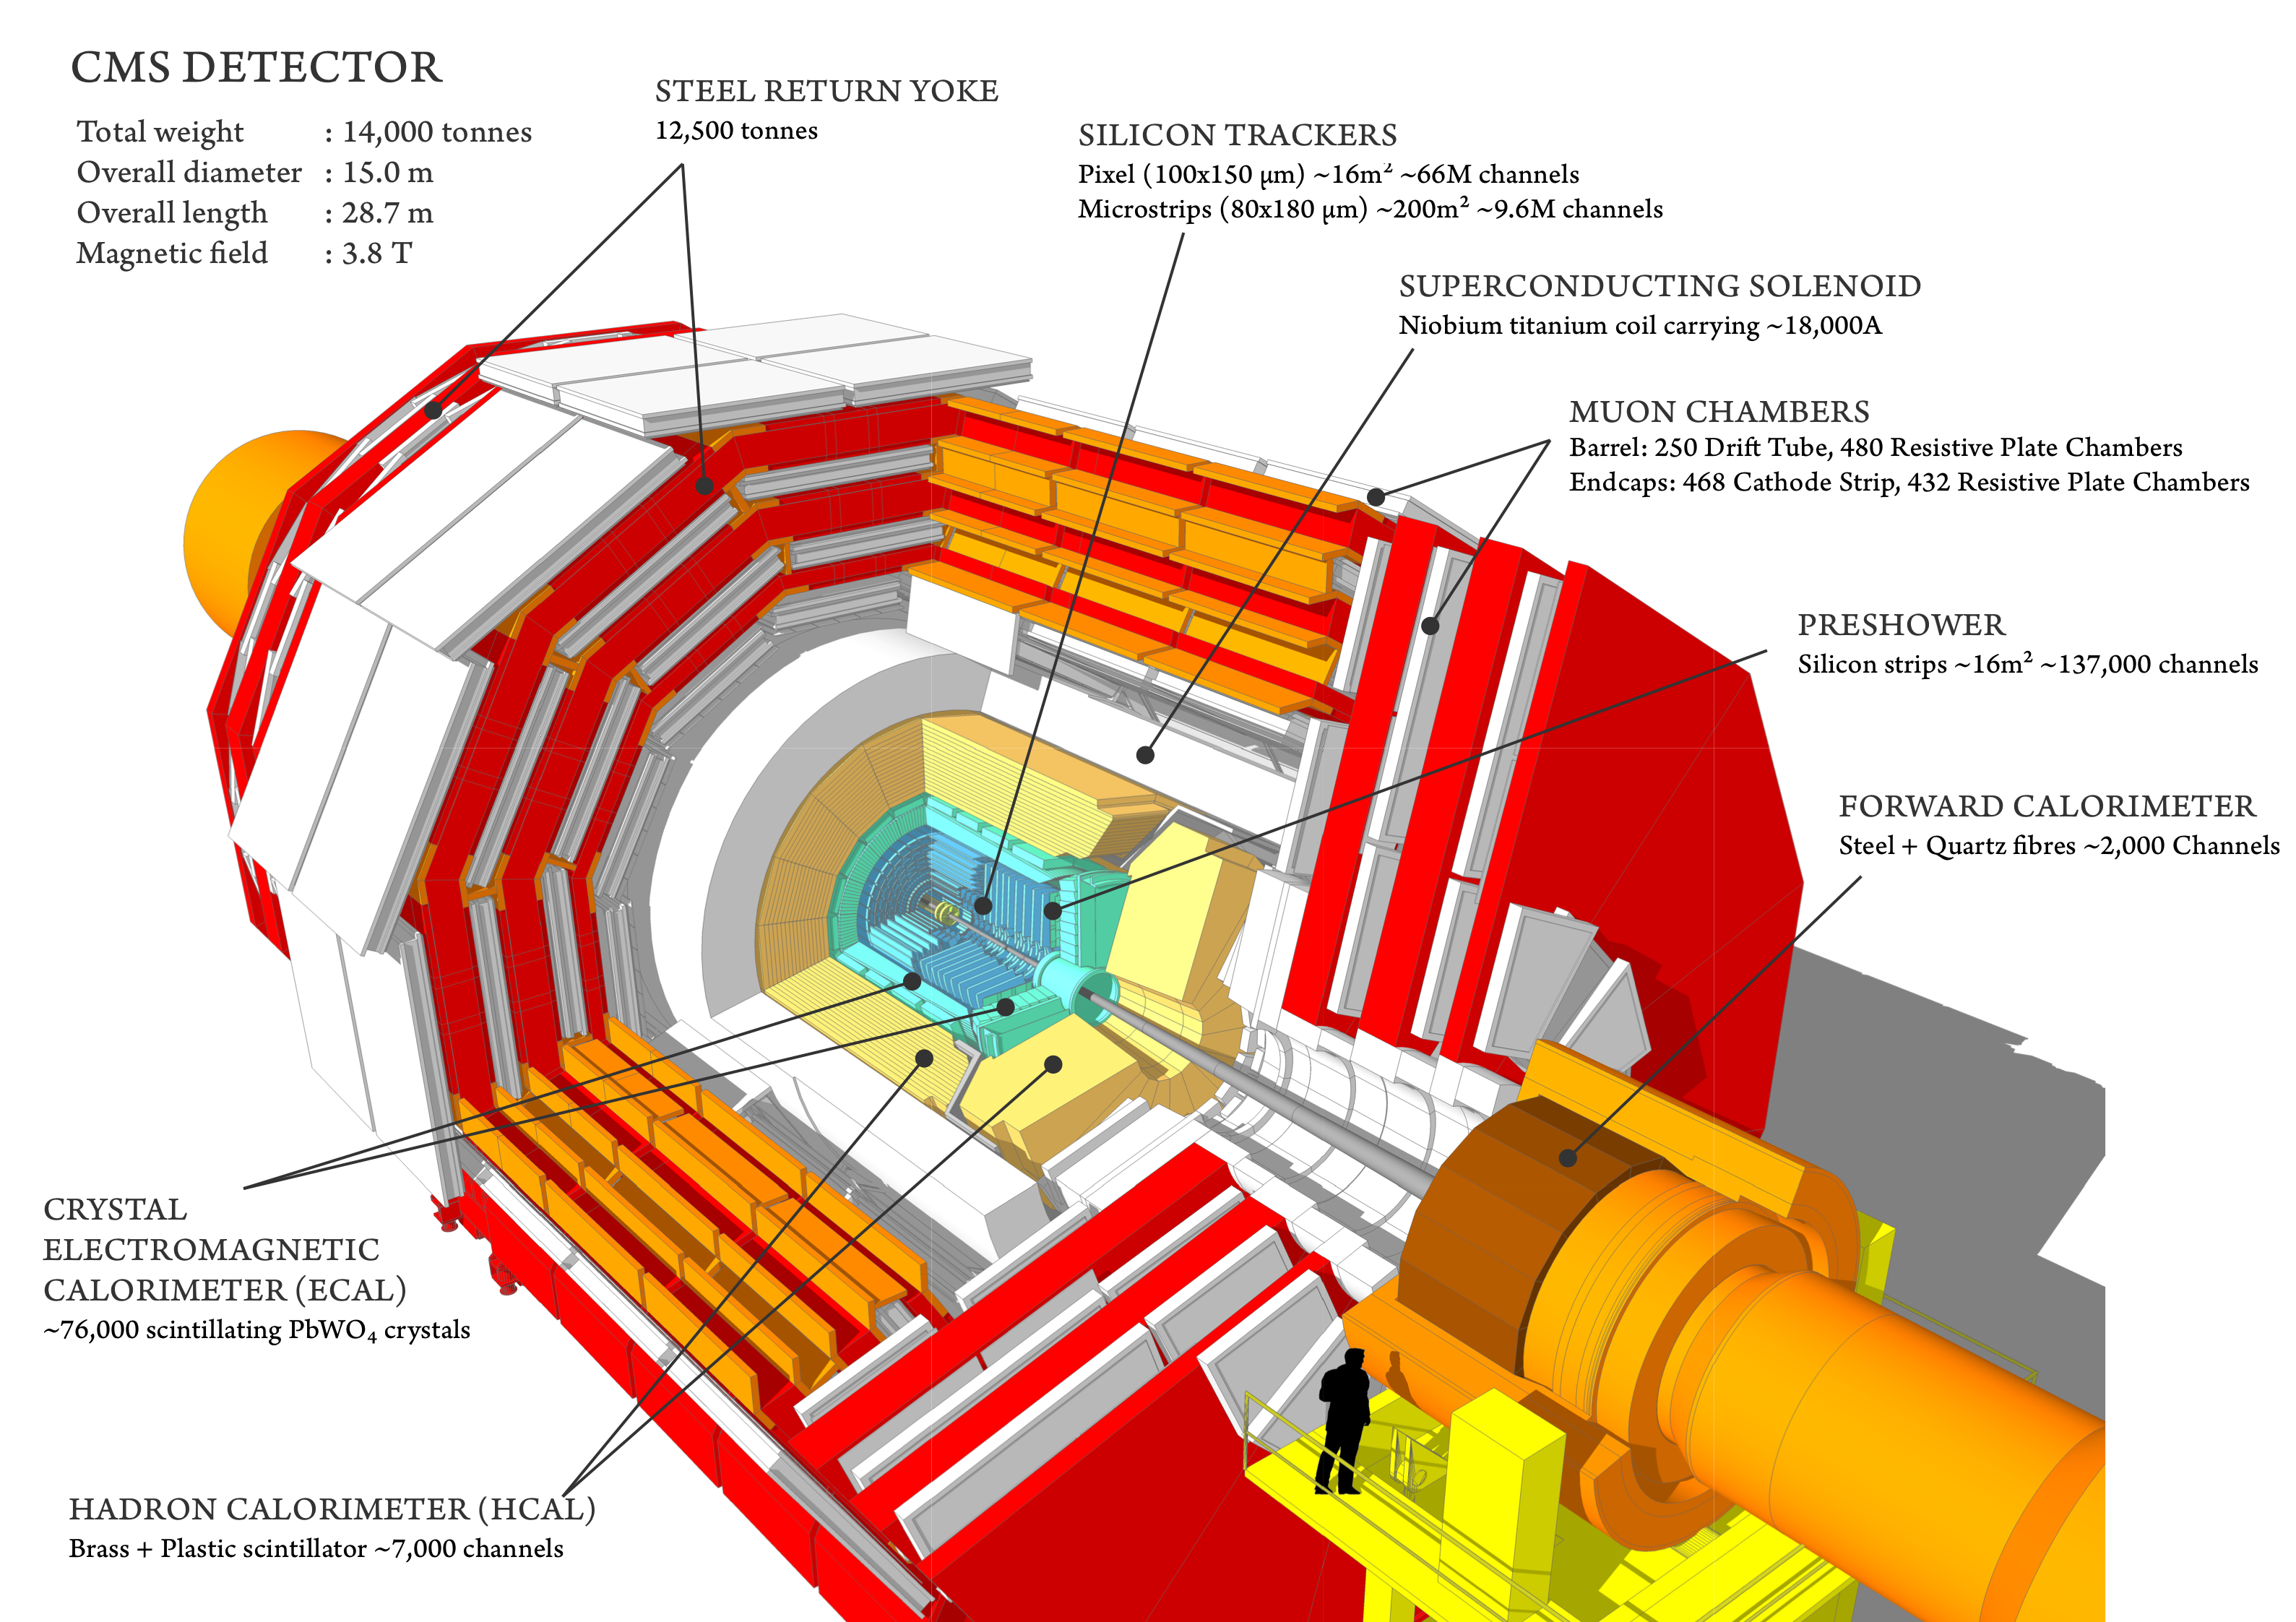
\includegraphics[width=1.2\largefigwidth]{plots/detector/cms_120918_03.png}
  \DIFdelbeginFL %DIFDELCMD < \caption{%%%
\DIFdelendFL \DIFaddbeginFL \caption[A diagram of the subsystems making up the CMS detector, illustrating the hermeticity and layered structure of the experiment.]{\DIFaddendFL A diagram of the subsystems making up the CMS detector, illustrating the hermeticity and layered structure of the experiment\DIFaddbeginFL \DIFaddFL{~}\DIFaddendFL \cite{cmsschematic}.}
  \label{fig:cmsschematic1}
\end{figure}

A central design feature of CMS is the superconducting magnet, inside which is generated a 3.8\DIFaddbegin \,\DIFaddend T axial field. This field bends the path of charged particles travelling through it allowing their momentum to be measured. Not all particles are charged however, and the path of several types of particles through the CMS detector is shown in \FigureRef{fig:cmsschematic2}. The first layer is the tracker which records the paths taken by charged particles\DIFdelbegin \DIFdel{, as }\DIFdelend \DIFaddbegin \DIFadd{. As }\DIFaddend well as providing a momentum measurement the tracks also allow the vertex from which the particle came to be identified. The next layer is the \ac{ECAL} where electrons and photons deposit energy through electromagnetic showers. This is followed by the \ac{HCAL} where hadrons deposit most of their energy. After the calorimetry systems is the superconducting magnet which is not instrumented. Outside the magnet are the muon detection systems, which are interspersed with iron plates which form the return yoke for the magnet. Due to their high mass compared to electrons, muons do not deposit much energy in the detector and often are not stopped, so the muon system is primarily a tracking detector.

\begin{figure}
  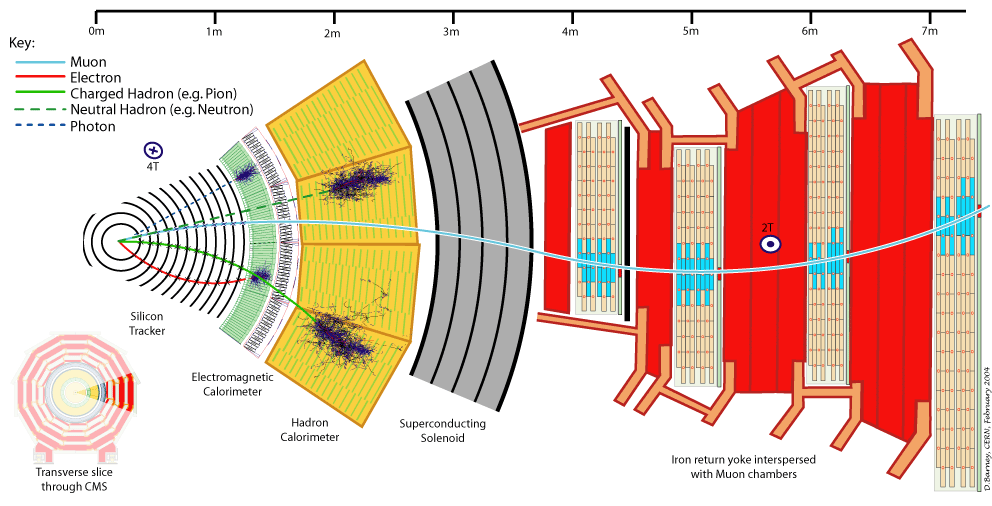
\includegraphics[width=1.2\largefigwidth]{plots/detector/CMS_Slice.png}
  \DIFdelbeginFL %DIFDELCMD < \caption{%%%
\DIFdelendFL \DIFaddbeginFL \caption[A schematic cross-section of the CMS experiment showing the path taken by several types of particles.]{\DIFaddendFL A schematic cross-section of the CMS experiment showing the path taken by several types of particles\DIFaddbeginFL \DIFaddFL{~}\DIFaddendFL \cite{CMSSlice}.}
  \label{fig:cmsschematic2}
\end{figure}

%Coordinate system
The origin of the co-ordinate system used by CMS is at the nominal interaction point. It is a right handed cartesian system with the \DIFdelbegin \DIFdel{x }\DIFdelend \DIFaddbegin \DIFadd{$x$ }\DIFaddend axis pointing towards the centre of the \LHC ring and the \DIFdelbegin \DIFdel{y-axis }\DIFdelend \DIFaddbegin \DIFadd{$y$-axis }\DIFaddend vertically upwards, the \DIFdelbegin \DIFdel{z }\DIFdelend \DIFaddbegin \DIFadd{$z$ }\DIFaddend axis then points along the beam line. The azimuthal angle $\phi$ and the polar angle $\theta$ are measured in radians from the \DIFdelbegin \DIFdel{x and z }\DIFdelend \DIFaddbegin \DIFadd{$x$ and $z$ }\DIFaddend axes respectively. It is common to describe the direction of outgoing particles using $\phi$ and their pseudo-rapidity, $\eta$ which is defined as:
\begin{equation}
  \label{eq:eta}
  \eta=-\ln[\tan(\theta/2)].
\end{equation}
Distances in the $\eta-\phi$ plane are given by $\Delta R=\sqrt{\Delta\phi^2+\Delta\eta^2}$. Two other quantities often used at hadron colliders are the projections of a particle's momentum and energy in the transverse plane, these are denoted as \pt and \Et respectively. The missing transverse energy, defined as the negative vector sum of the momentum in the transverse plane of all particles in an event, is important in inferring the presence of invisible particles and is denoted \MET. Also, when describing an event the terms \DIFdelbegin \DIFdel{leading and }\DIFdelend \DIFaddbegin \DIFadd{``leading'' and ``}\DIFaddend sub-leading\DIFaddbegin \DIFadd{'' }\DIFaddend refer to the highest and second-highest \pt objects in an event respectively.

\subsection{Tracker}
\label{sec:tracker}
%Describe Tracker http://dx.doi.org/10.1140/epjcd/s2004-03-1801-1 and jinst paper
The tracker is designed to measure the paths of charged particles precisely from \LHC collisions which curve in CMS's magnetic field. The design transverse momentum resolution of the full tracking detector is 1-2\% at 100\GeV~. In order to measure the particles' positions precisely and ensure the occupancy of the tracker is low a high granularity is required. Due to the frequency of collisions at the \LHC and the high instantaneous luminosity a radiation hard system with fast response is also necessary. This combination of requirements motivates the use of a \DIFdelbegin \DIFdel{silicon based }\DIFdelend \DIFaddbegin \DIFadd{silicon-based }\DIFaddend system. When traversing silicon charged particles create electron-hole pairs, which are then separated by an applied electric field, causing a current pulse.

%Submodules
%pixel
The tracker layout can be seen in \FigureRef{fig:trackerschematic}. In order to keep the sensor occupancy below 1\% at design luminosity, the innermost component is a silicon pixel detector. This detector has three layers in the barrel, at radii of 4.7, 7.3 and 10.2 cm, and two in the endcap. The are 66 million pixels each 100\DIFaddbegin \,\DIFaddend \micron\,\DIFdelbegin \DIFdel{x }\DIFdelend \DIFaddbegin \DIFadd{$\times$ }\DIFaddend 150\DIFaddbegin \,\DIFaddend \micron\,in size. The resulting resolution of the pixel detector is approximately 10\DIFaddbegin \,\DIFaddend \micron\,in the $r-\phi$ plane and 17\DIFaddbegin \,\DIFaddend \micron\,in the $r-z$ plane \cite{trackerperformance}. During \DIFdelbegin \DIFdel{run }\DIFdelend \DIFaddbegin \DIFadd{Run }\DIFaddend 1 the proportion of modules in the pixel (strip) tracker known to be defective was 2.4\% (2.3\%)~\cite{Chatrchyan:1704291}.

\begin{figure}
  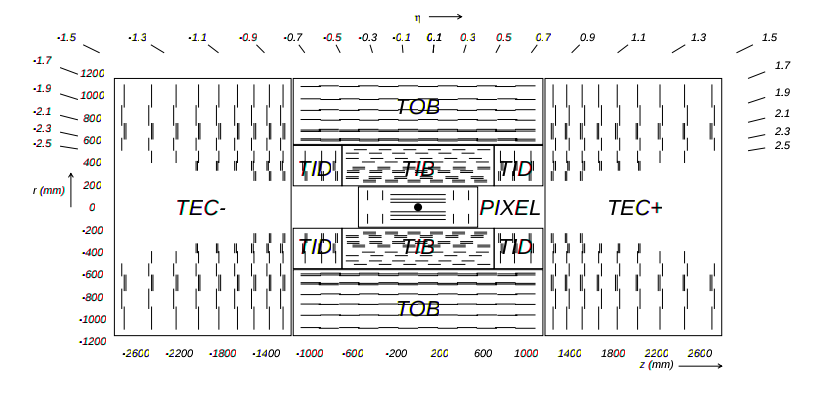
\includegraphics[width=1.2\largefigwidth]{plots/detector/TrackerSchematic.png}
  \DIFdelbeginFL %DIFDELCMD < \caption{%%%
\DIFdelendFL \DIFaddbeginFL \caption[A cross-section of the CMS tracker, indicating the subsystems that comprise it. Each line indicates a detector module and the labels for each subsection are the names given by CMS to the various subsections of the tracker.]{\DIFaddendFL A cross-section of the CMS tracker, indicating the subsystems that comprise it. Each line indicates a detector module\DIFaddbeginFL \DIFaddFL{~}\DIFaddendFL \cite{Chatrchyan:2008aa} and the labels for each subsection are the names given by CMS to the various subsections of the tracker.}
  \label{fig:trackerschematic}
\end{figure}



%strip
Surrounding the pixel detector is a silicon strip detector with 10 layers in the barrel, at radii of 20 to 116 cm, and 12 pairs of disks in the endcap. The strips are typically 10-20 cm long and 80-180\DIFaddbegin \,\DIFaddend \micron\,wide, with the strip size increasing with radius as the particle flux decreases. The strip detector's single point resolution is 230-530\DIFaddbegin \,\DIFaddend \micron\,in the $r-z$ plane and 23-52\DIFaddbegin \,\DIFaddend \micron\,in the $r-\phi$ plane.  The better resolution in the $r-\phi$ plane allows \pt to be measured with higher precision, as this is the direction in which a particle's track bends in the CMS magnetic field. The barrel and endcap detectors together have an acceptance of $|\eta|<2.5$ for both the pixel and strip detectors. Further details on the position resolution of the tracking detector for vertex reconstruction will be given in \SectionRef{sec:PV}.

\subsection{Electromagnetic calorimeter}
\label{sec:ECAL}
%Describe \ac{ECAL}
The \ac{ECAL} is designed to provide accurate photon and electron reconstruction and precise measurement of the electromagnetic component of hadron jets. It is a homogeneous calorimeter made of lead tungstate (PbWO$_{4}$) crystals, separated into a barrel section, with 61200 crystals and two endcaps each with 7234 crystals. These crystals are 25.8 radiation lengths in depth in the barrel and instrumented with photodetectors \DIFdelbegin \DIFdel{, avalanche photodiodes being used }\DIFdelend \DIFaddbegin \DIFadd{(avalanche photodiodes }\DIFaddend in the barrel and vacuum phototriodes in the endcap\DIFaddbegin \DIFadd{)}\DIFaddend . 

The layout of the \ac{ECAL} is shown in \FigureRef{fig:ecalschematic}. The \ac{EB} crystals have a \DIFdelbegin \DIFdel{170x360 }\DIFdelend \DIFaddbegin \DIFadd{170$\times$360 }\DIFaddend arrangement in $\eta-\phi$ space such that the gaps between crystals are offset by $3^{\circ}$ from the vector to the detector origin, thus avoiding particles travelling through the gaps. The \ac{EB} extends to $|\eta|=1.479$, with higher values of $\eta$ covered by the \ac{EE}. The crystals in the \ac{EE} are arranged in an $x-y$ grid pointing at a focus 1.3\DIFaddbegin \,\DIFaddend m from the nominal interaction point, giving a \DIFdelbegin \DIFdel{$2-8^{\circ}$ }\DIFdelend \DIFaddbegin \DIFadd{$2^{\circ}-8^{\circ}$ }\DIFaddend separation between the gaps between crystals and the vector to the detector origin. In addition to the main PbWO$_{4}$ detector the endcaps also have a preshower detector. This preshower is a lead silicon strip sampling calorimeter, which initiates the electromagnetic showers and provides sufficient position resolution to distinguish single photons from pairs produced in neutral pion decays. The total acceptance of the barrel and endcap detectors is $|\eta|<3.0$.

\begin{figure}
  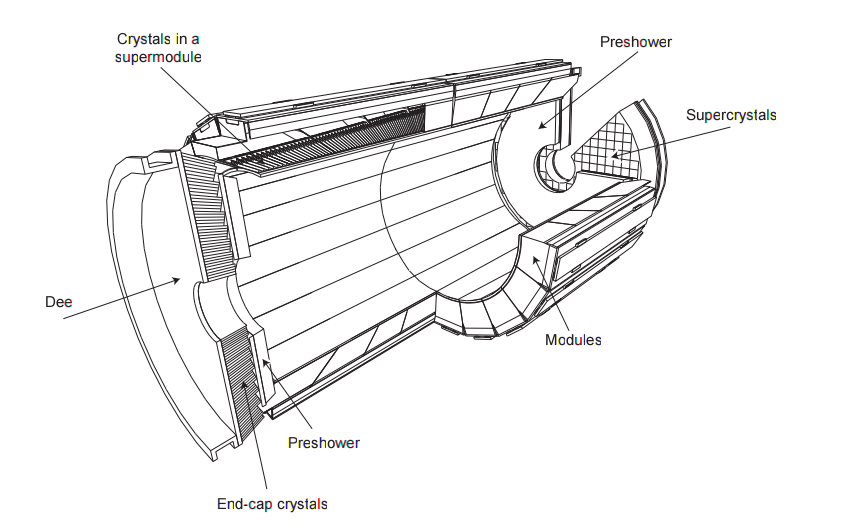
\includegraphics[width=1.2\largefigwidth]{plots/detector/ecal_layout.png}
  \DIFdelbeginFL %DIFDELCMD < \caption{%%%
\DIFdelendFL \DIFaddbeginFL \caption[A schematic of the CMS ECAL, indicating the subsystems that comprise it. The ECAL is 7.8\,m long by 3.5\,m wide.]{\DIFaddendFL A schematic of the CMS \DIFdelbeginFL %DIFDELCMD < \ac{ECAL}%%%
\DIFdelendFL \DIFaddbeginFL \DIFaddFL{ECAL}\DIFaddendFL , indicating the subsystems that comprise it. The \DIFdelbeginFL %DIFDELCMD < \ac{ECAL} %%%
\DIFdelendFL \DIFaddbeginFL \DIFaddFL{ECAL }\DIFaddendFL is 7.8\DIFaddbeginFL \,\DIFaddendFL m long by 3.5\DIFaddbeginFL \,\DIFaddendFL m wide\DIFaddbeginFL \DIFaddFL{~}\DIFaddendFL \cite{Chatrchyan:2008aa}.}
  \label{fig:ecalschematic}
\end{figure}

 On entering the \ac{ECAL} high energy electrons or photons initiate an electromagnetic shower by undergoing Bremsstrahlung or pair production respectively. The resulting cascade of particles continues to lose energy by successive Bremsstrahlung and pair production until their energy is low enough that the photons no longer undergo pair-production and the electrons lose their energy mainly by ionisation. The excitation of the PbWO$_{4}$ crystals leads to the emission of scintillation light, proportional to the amount of energy deposited, which is collected by the photodetectors.

The choice of PbWO$_{4}$ is motivated by its high density (8.28 g/cm$^{3}$), short radiation length (0.89 cm), small Moli\'{e}re radius (2.2\DIFaddbegin \,\DIFaddend cm) and radiation hardness. These properties lead to the showers being contained in a small area and allows the calorimeter to be compact and have fine granularity. Another advantage of PbWO$_{4}$ is that 80\% of the scintillation light is emitted within the LHC's \DIFdelbegin \DIFdel{25ns design bunch crossing }\DIFdelend \DIFaddbegin \DIFadd{25}\,\DIFadd{ns design bunch-crossing }\DIFaddend time, so particles can be properly associated with the \DIFdelbegin \DIFdel{bunch crossing }\DIFdelend \DIFaddbegin \DIFadd{bunch-crossing }\DIFaddend from which they originate.

%Resolution
For particle energies below 500 \DIFdelbegin \DIFdel{GeV, where the resulting shower ceases }\DIFdelend \DIFaddbegin \GeV\DIFadd{, for which the resulting showers are }\DIFaddend to be contained in the full depth of the \ac{ECAL}, the \ac{ECAL} resolution can be parameterised as:
\begin{equation}
  \label{eq:ecalres}
  \left(\frac{\sigma}{E}\right)^2=\left(\frac{S}{\sqrt{E}}\right)^2+\left(\frac{N}{E}\right)^2+C^2.
\end{equation}
Where $S$ is the stochastic term, $N$ the noise term and $C$ the constant term. The stochastic term is comprised of fluctuations in the lateral containment of showers and also in the amount of scintillation light. The noise term is made up of electronic and digital noise, and signals from other bunch crossings which do not fully dissipate in time. The constant term comes from non-uniformity of light collection along the crystals, errors in the calibration of crystals against each other and leakage of energy from the back of the calorimeter. The energy resolution was measured without an applied magnetic field in an electron beam using particles with momenta between 20 and 250\DIFaddbegin \,\DIFaddend \GeV. The stochastic, noise and constant terms were found to be 0.028 $\GeV^{1/2}$, 0.12\DIFaddbegin \,\DIFaddend \GeV and 0.003 respectively.

As the \ac{ECAL} is exposed to radiation the PbWO$_{4}$ crystals darken and as a result fewer photons are collected per unit energy deposited. The loss of response due to this darkening at the end of Run I varies from 6\% for crystals in the most central region of the \ac{ECAL} to 30\% in the endcaps~\cite{CMS-DP-2015-063}.

 

\subsection{Hadronic calorimeter}
\label{sec:HCAL}
%Describe HCAL
The \ac{HCAL} is designed to measure the energy of strongly interacting particles. This measurement is particularly important for neutral hadrons which do not leave tracks in the tracking system and deposit most of their energy in the \ac{HCAL}, and for the determination of \MET.  The main part of the \ac{HCAL} consists of a brass and scintillator plus wavelength shifting fibre sampling calorimeter split into \ac{HB} and \ac{HE} sections. The primary design consideration for the \ac{HCAL} is that it must fit between the outer edge of the \ac{ECAL} ($r=1.77$ m) and the inner edge of the magnet ($r=2.95$ m). In order to satisfy this requirement and achieve satisfactory containment of hadronic showers the magnet coil is also used as an absorber, and there is a further layer of scintillator outside the magnet coil (\ac{HO}). The barrel and endcap detectors extend to $|\eta|<3$.

Brass is chosen as the main \ac{HCAL} absorber because it is not magnetic and has a relatively short nuclear interaction length of 16.42 cm. Once showers have been initiated in the absorber layers they then pass through the plastic scintillator tiles, where they create pulses of light. These pulses are transferred via wavelength shifting fibres to hybrid photodiodes. The segmentation of the scintillator is such that the $\eta-\phi$ resolution in the \ac{HB} (\ac{HE}) is $0.087\times 0.087$ (between $0.087\times 0.087$ and $0.17\times 0.17$ depending on $\eta$).

In addition to the barrel and endcap sections of the \ac{HCAL} there is also a steel and quartz fibre Cherenkov forward calorimeter (\ac{HF}), which extends the calorimetry coverage of CMS to $|\eta|<5.2$. The choice of this technology is driven by its ability to withstand the very high particle fluxes present so close to the beamline. Showers are initiated by the steel absorber and signals are generated in the quartz fibres by particles above the Cherenkov threshold generating Cherenkov light, which is collected by photomultiplier tubes. Due to the Cherenkov energy threshold increasing with particle mass the \ac{HF} is primarily sensitive to the electromagnetic component of showers.

A diagram of the \ac{HCAL} layout can be seen in \FigureRef{fig:hcalschematic}. In total the \ac{HCAL} corresponds to 10-15 interaction lengths, depending on $\eta$. The resolution of the barrel and endcap sections of the \ac{HCAL} as a function of the incident particle energy was measured in a pion beam and has been found to be well parameterised by:
\begin{equation} 
  \label{eq:hcalres}
  \left(\frac{\sigma}{E}\right)^{2}=\left(\frac{94.3\%}{\sqrt{E}}\right)^{2}+\left(8.4\%\right)^{2}~\cite{Abdullin:2009zz}.
\end{equation}

\begin{figure}
  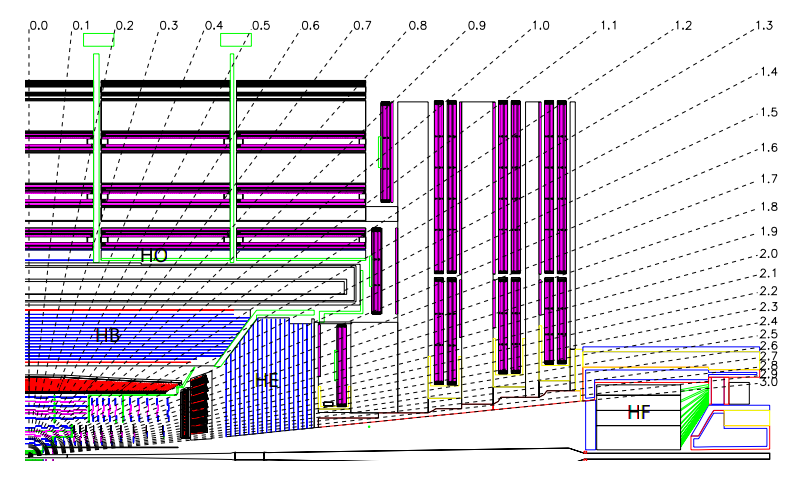
\includegraphics[width=1.2\largefigwidth]{plots/detector/hcal_layout1.png}
  \DIFdelbeginFL %DIFDELCMD < \caption{%%%
\DIFdelendFL \DIFaddbeginFL \caption[A schematic of a quadrant of the CMS HCAL in the $r-z$ plane, indicating the subsystems that comprise it.]{\DIFaddendFL A schematic of a quadrant of the CMS \DIFdelbeginFL %DIFDELCMD < \ac{HCAL} %%%
\DIFdelendFL \DIFaddbeginFL \DIFaddFL{HCAL }\DIFaddendFL in the $r-z$ plane, indicating the subsystems that comprise it\DIFaddbeginFL \DIFaddFL{~}\DIFaddendFL \cite{Chatrchyan:2008aa}.}
  \label{fig:hcalschematic}
\end{figure}

\subsection{Muon system}
%Describe muon system
As described above muons are highly penetrating, and thus are only rarely contained by the inner detector. Very few other charged particles are able to leave the calorimeters \DIFaddbegin \DIFadd{without being absorbed}\DIFaddend , so the presence of tracks in the muon system is sufficient to identify muons. The muon tracking system uses three types of gaseous particle detectors, located throughout the iron magnet return yoke. In all three types of detector when a charged particle travels through the gaseous detector it ionises the gas, the resulting free electrons then drift towards the detector's anode resulting in an electrical signal. The two primary types of detectors used are the \ac{DT}, which is used in the barrel section of the detector ($|\eta|<1.2$), and the \ac{CSC}, which is used in the endcap ($0.9<|\eta|<2.4$). The \ac{DT} and \ac{CSC} systems identify muons and provide measurements of their momentum. These measurements can be combined with those from the tracker to improve the muon momentum resolution. This combined reconstruction and momentum measurement along with its resolution is described in \SectionRef{sec:muons}. Additionally there is a \ac{RPC} system in both the barrel and endcap regions ($|\eta|<1.6$), the primary purpose of which is to provide trigger and \DIFdelbegin \DIFdel{bunch crossing }\DIFdelend \DIFaddbegin \DIFadd{bunch-crossing }\DIFaddend identification information. A diagram of the CMS muon system can be found in \FigureRef{fig:muonschematic}.

%DT
Each system has its own particular advantages and disadvantages which make it best suited for use in the various parts of the muon system. \ac{DT}s are inexpensive and reliable, but they are not usable in regions with high muon and neutron background rates, making them well suited to the barrel portion of the detector, where large areas must be instrumented and rates are low. Each \ac{DT} is a 2.4\DIFaddbegin \,\DIFaddend m long wire in a $13\times 42$\DIFaddbegin \,\DIFaddend mm$^{2}$ tube. The length is limited by the segmentation of the iron return yoke, and the cross-section by the requirement that the occupancy and drift time are low enough to prevent multiple muon hits being read out at the same time. The \ac{DT}s are organised in 4 stations, interspersed with return yoke iron plates. The first three stations have 8 chambers each, 4 to measure the muon's position in the $r-\phi$ plane and 4 to measure the $z$ co-ordinate. The final outermost layer does not have the $z$-measuring chambers. These chambers consist of 8-12 stacked \ac{DT}s, with each layer offset from the previous one by half the width of a tube to avoid gaps.

%CSC
Due to their fast response time, fine segmentation and radiation resistance \ac{CSC}s are ideal for the endcap region where the muon and background rates are higher. Each \ac{CSC} is a multiwire proportional chamber with 7 planes of cathode strips running radially outwards with 6 planes of anode wires, which run azimuthally, interleaved between them. Both the anode and cathode wires are read out to provide $\eta$ and $r-\phi$ co-ordinate measurements respectively. Similarly to the \ac{DT} system the design number of \ac{CSC} stations in each endcap is 4 interspersed with iron return yoke plates. During Run \DIFdelbegin \DIFdel{I }\DIFdelend \DIFaddbegin \DIFadd{1 }\DIFaddend only three of the \ac{CSC} stations were present\DIFdelbegin \DIFdel{, }\DIFdelend \DIFaddbegin \DIFadd{; }\DIFaddend the fourth station in each endcap was added during the long shutdown and is present for Run 2. The position resolution in the $r-\phi$ plane of the \ac{CSC}s varies from 75-80\DIFaddbegin \,\DIFaddend \micron.

%RPC
The \ac{RPC}s are gas gaps surrounded by anode and cathode plates with read out strips between them. The advantage of \ac{RPC}s is that their response is good at high rates, and they have very good time resolution, making them ideal for use in the trigger and assignment of muons to a bunch crossing. However, they have much poorer position resolution than the \ac{DT}s or \ac{CSC}s. There are 6 layers of \ac{RPC}s in the barrel and 3 in the endcap.

\begin{figure}
  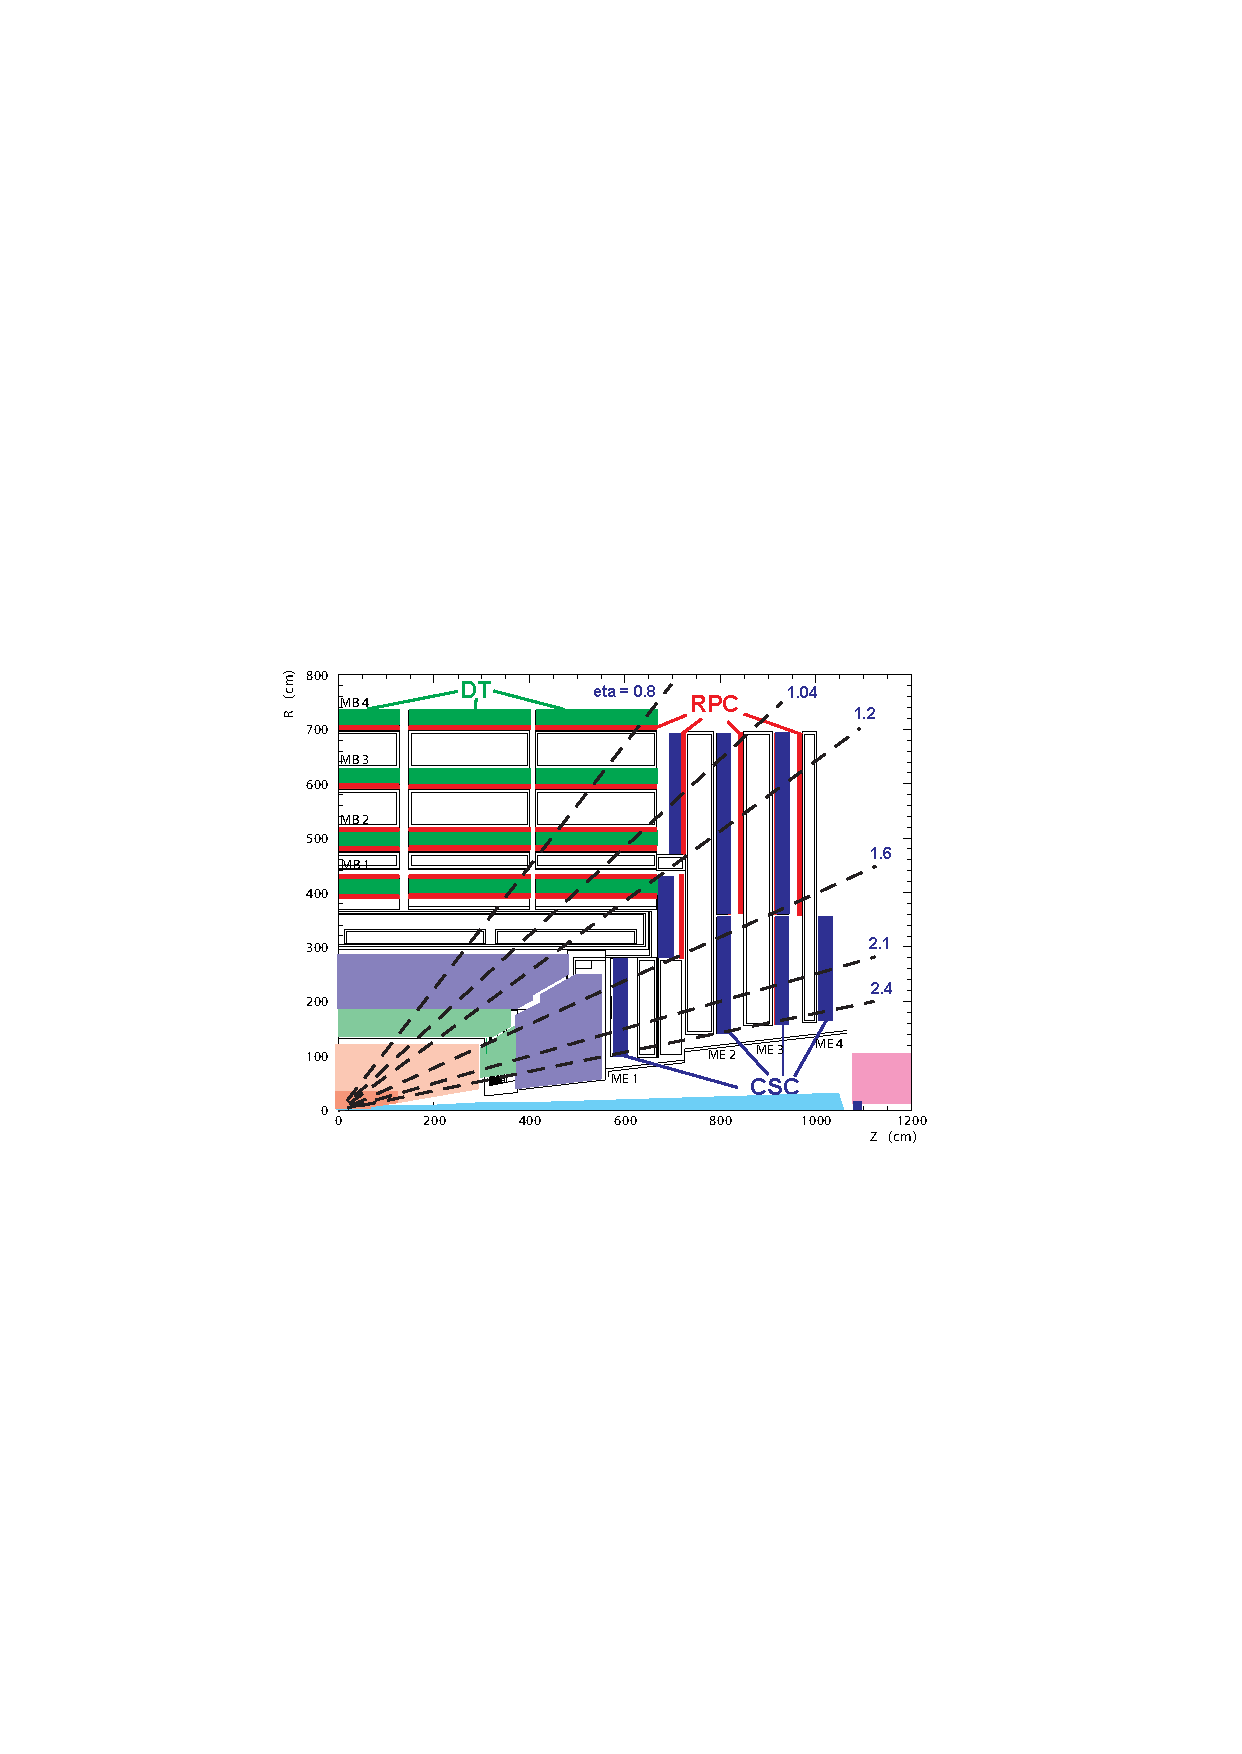
\includegraphics[width=1.2\largefigwidth]{plots/detector/muon_layout.pdf}
  \DIFdelbeginFL %DIFDELCMD < \caption{%%%
\DIFdelendFL \DIFaddbeginFL \caption[A schematic of a quadrant of the CMS muon system in the $r-z$ plane, indicating the subsystems that comprise it.]{\DIFaddendFL A schematic of a quadrant of the CMS muon system in the $r-z$ plane, indicating the subsystems that comprise it\DIFaddbeginFL \DIFaddFL{~}\DIFaddendFL \cite{Bayatian:922757}.}
  \label{fig:muonschematic}
\end{figure}

\subsection{Trigger system}
\label{sec:triggers}
%Describe trigger system
The design bunch crossing rate of the \LHC is 40 MHz, and for the data used in this thesis it \DIFdelbegin \DIFdel{varied from 20-40 }\DIFdelend \DIFaddbegin \DIFadd{was either 20 or 40 }\DIFaddend MHz. Since each event consists of approximately 1 MB of data, writing every event to tape would correspond to a data rate of 20-40 TB$/s$ which is not feasible. It is also not feasible for the detector electronics to read out the detector at this frequency. It is therefore necessary to use a trigger system to perform an ``online'' reconstruction and reduce the event rate by selecting only the most interesting events.

The trigger is separated into two stages, the \ac{L1} trigger and the \ac{HLT}. First the \ac{L1} trigger, which is built of custom-designed electronics, reduces the rate to a maximum of 100 kHz. The decision to accept an event in the \ac{L1} trigger or not starts with local information on the energy deposits in the calorimeters and hits in the muon systems, which is stored for all events for 128 bunch crossings. A decision must therefore be made within 128 bunch crossings or the event is discarded. Due to the limited time available and the limited available bandwidth of the data acquisition system, this information is generally not available at the detector's full resolution. After it is collected from the detector the local information is then passed to the regional trigger systems, which generate lists of trigger candidates, such as electrons or jets, ranked by energy and quality. These ranked lists from each region are then passed to the global muon and calorimeter system triggers, which select the highest ranked candidates across the whole detector and give them to the global trigger, which makes a final decision. This process is shown in \FigureRef{fig:l1layout}.

\begin{figure}
  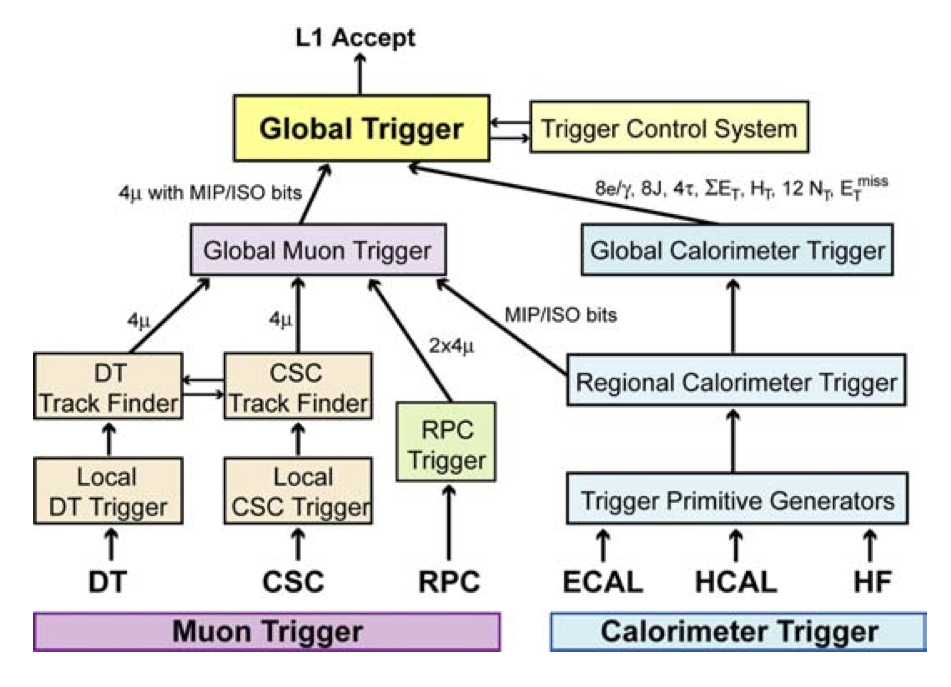
\includegraphics[width=1.2\largefigwidth]{plots/detector/L1T_Layout.png}
  \DIFdelbeginFL %DIFDELCMD < \caption{%%%
\DIFdelendFL \DIFaddbeginFL \caption[A schematic of the L1 trigger system. The arrows indicate the flow of data, the information transferred between systems is also indicated.]{\DIFaddendFL A schematic of the \DIFdelbeginFL %DIFDELCMD < \ac{L1} %%%
\DIFdelendFL \DIFaddbeginFL \DIFaddFL{L1 }\DIFaddendFL trigger system. The arrows indicate the flow of data, the information transferred between systems is also indicated\DIFaddbeginFL \DIFaddFL{~}\DIFaddendFL \cite{Chatrchyan:2008aa}.}
  \label{fig:l1layout}
\end{figure}

If an event is accepted by the \ac{L1} trigger the full detector information is read out to the \ac{HLT} farm on the surface, which reduces the rate further still to approximately 1 kHz.  The \ac{HLT} consists of several thousand commercially available CPUs. Despite having the full detector information, the time available does not allow for the full offline reconstruction to be performed. \DIFdelbegin \DIFdel{Never the less}\DIFdelend \DIFaddbegin \DIFadd{Nevertheless}\DIFaddend , the algorithms available at the \ac{HLT} are much closer to those used offline than those available at \ac{L1}, allowing the trigger to better select events that would also pass requirements on the offline quantities. If they are accepted by the \ac{HLT}, events are sent to be reconstructed using the \ac{WLCG}. 

\subsection{Data processing}
The \ac{WLCG} consists of several tiers. Data is first fully reconstructed at the Tier 0 centres. During Run I there was only one of these at CERN, for Run II there will also be a Tier 0 centre in Budapest. It is then sent to at least one Tier 1 centre, so that a full copy of the data is available at multiple sites in different geographic locations. Tier 2 and 3 centres then process this data according to the needs of specific analyses.

During 2012 running it was realised that it was possible for data to be written to tape from the CMS detector at a higher rate than it could be reconstructed by the Tier 0. 30\% of the output of CMS was therefore immediately sent for ``prompt'' reconstruction, while the remainder was ``parked'' to tape to be reconstructed during \LHC shutdown periods when there is spare computing capacity available \cite{CMS-DP-2012-022}. The extra events that could be stored through this parking allowed significantly lower trigger selection thresholds to be used for some of the analyses described in this thesis.


\chapter{Physics objects and event reconstruction}
\label{chap:obj}
%Introduce reconstruction
The invisible Higgs analysis uses a wide range of objects from the jets and \MET that are present in the signal process, to charged leptons that are present in background processes. This range of objects means that information from all the CMS subdetectors must be used. The reconstruction of each physics object used from data collected by the CMS detector is described in this chapter, along with the overarching ``particle flow'' approach to data reconstruction used by CMS.

\section{Tracks}
\label{sec:tracks}
%This and next section from http://iopscience.iop.org/article/10.1088/1748-0221/9/10/P10009/pdf
The tracks reconstructed in the inner tracking detector of CMS are a key part of the reconstruction of most other objects used for physics analyses. For example the jet reconstruction algorithm combines information from the tracks and calorimeter energy deposits. The algorithm used by CMS is the Kalman filter based \ac{CTF}, which is described in \ReferenceRef{1748-0221-9-10-P10009}. 

The \ac{CTF} starts with seeds generated from either two or three hits in the pixel tracker. Seeds with two hits use the nominal crossing point of the beams to constrain the initial momentum of the track. The layers of the tracker are then iterated through, from inside to outside. The most compatible hit in each layer is added to the track and the track is refitted before moving to the next layer. Once the outside of the detector is reached the algorithm checks for tracks which share more than 19\% of their hits and discards the track with the fewest hits. In the case of the two tracks having an equal number of hits the track with the best fit, i.e. that having the lowest $\chi^{2}$, is kept. This process of reconstructing tracks starting from seeds is repeated up to six times, with hits associated to a successfully reconstructed track removed for the next iteration. 

After the full set of iterations is complete the tracks are refitted again using another Kalman filter, initialised with the innermost hit on the track and proceeding to iteratively add the hits on the track from inside to outside. This refitting aims to reduce biases from the track's seed including those introduced for \DIFdelbegin \DIFdel{two hit }\DIFdelend \DIFaddbegin \DIFadd{two-hit }\DIFaddend seeds that include constraints from the beamspot. The refitted tracks are then smoothed by another Kalman filter, which is initialised with the current \DIFdelbegin \DIFdel{best fit }\DIFdelend \DIFaddbegin \DIFadd{best-fit }\DIFaddend track hypothesis and iterates from the outside of the detector inwards. 

The smoothed tracks then have quality criteria, such as a requirement on the maximum number of layers the track traverses without leaving a hit, imposed to reject fake tracks. The efficiency of the \ac{CTF} is estimated in data using tracks from muons from Z decays, and is found to be greater than 99\% for muons with $1<\pt<100$ \GeV. For muons with $\pt=100 \GeV$ the \pt resolution of the \ac{CTF} is found to be approximately 2.8\%~\cite{1748-0221-9-10-P10009}.

\section{Primary vertex}
\label{sec:PV}
%Describe PV reconstruction
%Relevance to analysis
%Check if hard scatter defined elsewhere
The very high instantaneous luminosities present at the \LHC lead to a large probability of multiple proton-proton interactions occurring in each bunch crossing. It is therefore essential to identify the \ac{PV}, which relates to the highest energy interaction or ``hard scatter''. It is also useful to identify the \ac{PV} to distinguish ``prompt'' particles directly from the hard scatter from those resulting from processes which occur later such as heavy flavour hadron decay or photon conversion.

%Algorithm
The CMS \ac{PV} reconstruction algorithm has three steps, track selection, clustering of tracks into vertices and finally fitting the position of these vertices and is described in more detail in \ReferenceRef{1748-0221-9-10-P10009}. In the first step, track selection, the subset of tracks with non-significant transverse impact parameters is chosen. This selection removes tracks not coming from the primary interaction region.

The next step of clustering tracks into prototype vertices uses a \ac{DA} algorithm~\cite{DetAnnealing}. These prototype vertices then have their position determined by an adaptive vertex fitter~\cite{adaptivevertex}. This fitter starts by performing a fit to the position of the vertex, then assigning weights, $w_{i}$ to each track according to the probability that it belongs to the vertex, before repeating the process iteratively. Both of these algorithms also use the concept of ``cooling,'' where the algorithm is performed repeatedly as a temperature parameter, which controls the size of fluctuations around the current state of the system, is gradually reduced, to increase the chance of finding the global best fit solution.

The number of degrees of freedom of the resulting vertex is defined as:
\begin{equation}
  \label{eq:vertdof}
  n_{dof}=2\displaystyle\sum_{i=1}^{\# \rm{tracks}}w_i -3.
\end{equation}
This variable is highly correlated with the number of tracks compatible with the vertex and can therefore be used to select vertices coming from true proton-proton interactions.

The \ac{PV} is defined to be the vertex with the highest sum of the squared \pt of all the tracks contributing to it. If there is no reconstructed vertex the nominal beam crossing point is used. In the analyses described in this thesis events are required to have a real vertex, which has $n_{dof}>4$ and a maximum displacement in the $z$-direction ($xy$-plane) direction from the centre of the detector of 24 cm (2 cm).

%Performance, make sure jet is defined in theory section
The performance of the vertex reconstruction algorithm has been measured using events with at least one jet with $\pt>20$ GeV~\cite{1748-0221-9-10-P10009}. The efficiency to reconstruct at least one primary vertex in these events is found to be greater than 99\% for vertices with at least three tracks. The position resolution is found to vary as a function of the number of tracks associated to the vertex, being approximately 100\DIFaddbegin \,\DIFaddend \micron\, for vertices with 5 tracks and approaching 10\DIFaddbegin \,\DIFaddend \micron\, for vertices with greater than 50 tracks.

\section{Particle flow}
\label{sec:pf}
%Describe pf reconstruction, Relevance to analysis
\ac{PF} is an algorithm used by CMS to combine information from different sub-detectors into individual particles~\cite{CMS-PAS-PFT-09-001,CMS-PAS-PFT-10-001,CMS-PAS-PFT-10-002}. This approach is particularly beneficial for CMS as it allows the accurate momentum measurements of the inner tracker, and the excellent energy measurements and granularity of the \ac{ECAL} to be combined and used to improve the energy measurement of objects seen in the \ac{HCAL}. The \ac{PF}\DIFaddbegin \,\DIFaddend approach also allows calibrations specific to charged and neutral hadrons to be applied. The \ac{PF} algorithm classifies particles as charged hadrons, neutral hadrons, photons, muons and electrons. This set of particles, referred to as \ac{PF} candidates, can then further be used to calculate the \MET, as input to the jet reconstruction, for reconstructing taus and to calculate the isolation of leptons.

%Algorithm
The \ac{PF} algorithm starts with tracks, reconstructed as described in \SectionRef{sec:tracks}, and calorimeter clusters, which are reconstructed separately in each sub-detector of the calorimeter system. Clustering starts with seeds, which are the calorimeter cells which have the local maximum energy which is also more than twice the expected calorimeter noise, which is 80 (300) \MeV\DIFaddbegin \, \DIFaddend in the \ac{EB} (\ac{EE}\DIFaddbegin \DIFadd{) }\DIFaddend and 800\DIFaddbegin \,\DIFaddend \MeV\DIFaddbegin \, \DIFaddend in the \ac{HCAL}. Cells adjacent to the cluster are added if they also have energy more than twice the expected calorimeter noise. Cluster-track pairs whose cluster position and track trajectory are compatible are then linked together to identify charged particles. Linking between tracks from the inner tracker and the muon system is also performed to identify muons. The information from tracks with associated \ac{ECAL} clusters, i.e. those compatible with electrons, is further used to search for clusters compatible with having come from Bremsstrahlung photons from the electron\DIFdelbegin \DIFdel{, }\DIFdelend \DIFaddbegin \DIFadd{; }\DIFaddend this is described further in \SectionRef{sec:electrons}.

Once electrons, muons and charged hadrons have been identified, further calorimeter clusters are identified as neutral hadrons or photons if they are in the \ac{HCAL} or \ac{ECAL} respectively. Excess energy in a calorimeter cluster compared to that expected from the associated tracks also allows the presence of neutral particles that would otherwise not have been identified to be determined.

\section{Electrons}
\label{sec:electrons}
%Describe electron reconstruction
As described in \SectionRef{sec:pf}, electrons are reconstructed by matching \ac{ECAL} deposits with tracks from the inner tracker. This process is complicated by the fact that electrons can lose significant amounts of energy, in the form of Bremsstrahlung photons, as they traverse the inner tracker. Approximately 35\% of electrons lose at least 70\% of their initial energy in this way~\cite{Baffioni:2006cd}. The Bremsstrahlung photons often convert to electron-positron pairs which are then further spread in the $\phi$ direction by CMS's solenoidal magnetic field. The electron reconstruction, which is described in detail in \ReferenceRef{1748-0221-10-06-P06005}, employs so-called ``supercluster'' algorithms to combine \ac{ECAL} deposits from both the initial electron and the Bremsstrahlung photons.

%supercluster forming and tracking
Due to their different geometries, different supercluster algorithms are used in the barrel and endcaps. In the barrel the ``hybrid'' clustering algorithm is used\DIFdelbegin \DIFdel{, }\DIFdelend \DIFaddbegin \DIFadd{: }\DIFaddend this begins with a seed crystal which is the crystal with local maximum energy greater than 1 \GeV. Arrays of 5$\times$1 crystals in $\eta\times\phi$ are then added around the seed crystal if they are within 17 crystals of it in either direction in $\phi$ and have energy greater than 0.1 \GeV. Contiguous arrays are grouped into clusters. The final supercluster consists of all clusters from a seed with cluster energy greater than 0.35 \GeV.

In the endcap the ``multi-5$\times$5'' algorithm is used. This algorithm also starts with seed crystals, in this case those with energy higher than their four direct neighbours and also greater than 0.18 \GeV. Clusters are then made up of the 5$\times$5 square of crystals centered on the seed. Individual clusters whose seeds are within 0.07 in $\eta$ and 0.3 \DIFaddbegin \DIFadd{radians }\DIFaddend in $\phi$ of each other are grouped and kept as a supercluster if their total energy is greater than 1\GeV. A reference position for the supercluster is taken to be the energy-weighted average position of all the clusters belonging to it, and the maximum difference in $\phi$ between any cluster and the reference position is taken to be the size of the cluster in $\phi$. The individual clusters in a supercluster are then extrapolated to the preshower detector. Any preshower deposits within the supercluster's $\phi$ size plus 0.15 in $\phi$ and within $0.15$ in $\eta$ of a cluster in the supercluster are added to it.

The energy-weighted average position and energy of the final supercluster are then used to extrapolate the electron's track back to the innermost layers of the tracker for both electron charge hypotheses. This extrapolation is then matched to hits within a $\phi - z$ window of it, whose size is determined by the uncertainties on the $\phi$ position of the supercluster and the $z$ position of the beamspot. This size was typically 5 cm in 2012. This matched hit is used to update the estimated electron trajectory so that a hit in the second layer of the inner tracker can be searched for in a much narrower window. Hits in both the first and second layers compatible with a supercluster are then used as seeds for dedicated electron track reconstruction, performed using a \ac{GSF} algorithm~\cite{GSFalgorithm}, which performs better than a Kalman Filter for tracks with significant energy loss.

%ID
Electron identification criteria are applied to reject fake electrons caused by other particles such as pions. The variables used include:
\begin{itemize}
\item $\Delta\eta_{in}$ and $\Delta\phi_{in}$, which are the $\eta$ and $\phi$ distances between the electron track position extrapolated to the \ac{ECAL} and the supercluster position.
\item $\sigma_{i\eta i\eta}$, the energy-weighted $\eta$ width of the cluster.
\item $H/E$, the ratio between the energy deposited in the \ac{HCAL} and in the \ac{ECAL} in the region of the electron's seed cluster.
\end{itemize}
All of these variables are generally lower for real prompt electrons.

We also require the electrons to be isolated, i.e. have a low amount of other activity present around them in the detector. The variable used for this requirement is the effective area corrected \ac{PF} isolation, $I_{PF}$. In Run 1 it was defined as the sum of the \pt of the \ac{PF} candidates within a cone of $\Delta R<0.4$ around the direction of the electron, minus the expected contribution from \ac{PU} across the area of the electron.

%Performance
In the \ac{VBF} invisible Higgs boson decay searches described later in this thesis two sets of requirements on the above variables are used to identify electrons, both of which require that $|\eta|<2.4$. The ``veto'' set of identification criteria is looser and is used to veto events containing electrons. The other ``tight'' set of criteria is stricter and is used when we want to study events containing electrons. Tight electrons are required to be separated by more than 0.3 in $\Delta R$ from any veto muons to remove fake electrons from muons. The veto (tight) criteria have an efficiency of 93\% (85\%) for reconstructing central electrons with $\pt>50$ GeV~\cite{eleeff}. The veto (tight) electrons used in the analyses described in this thesis are required to have \pt$>10 (20)$ \GeV unless stated otherwise.

\section{Muons}
\label{sec:muons}
%Describe muon reconstruction %Relevance to analysis
Due to their relatively high mass and lack of strong force interactions, most muons deposit very little energy in the CMS calorimeters and thus leave the detector after passing through the muon system. As described in \SectionRef{sec:pf}, this means that muons can be reconstructed by searching for compatible tracks from the inner tracker and the muon system. The approach of requiring both inner tracker and muon system tracks greatly improves the discrimination between muons and hadronic activity and is referred to as ``global'' muon reconstruction.

%Algorithm
The CMS global muon reconstruction algorithm starts with each track in the muon system and searches for compatible tracks in the inner tracker ~\cite{MuonReco}. If a compatible inner tracker track is found, a track fit, similar to that described in section \SectionRef{sec:tracks}, is performed using the hits in both the inner tracker and muon system. The fit accounts for energy losses as the muon traverses the detector. It is found that for muons with $\pt>200$\GeV the global-muon fit is better than that from the tracker only~\cite{MuonReco}. However, due to the increased hadron discrimination described above all muons used for analyses in this thesis are required to have both inner tracker and muon system tracks. As with electrons it is also required that muons are isolated. The same isolation variable, $I_{PF}$, as described in \SectionRef{sec:electrons} is used for muon isolation. Global muon reconstruction is sufficient for use in vetoing events containing muons, and muons passing the above reconstruction are referred to as ``veto'' muons.

Where we want to study events containing muons, further identification criteria are used. This is because whilst global muon reconstruction removes most hadrons, some so-called ``punch through'' hadrons, which are energetic enough to travel all the way through the CMS calorimeters, can still be reconstructed as muons. Furthermore, it is desirable to separate real but non-prompt muons from hadron decay, from prompt muons from the hard scatter or tau decay. The identification consists of requiring a high quality global muon track fit, that the muon's track passes through at least \DIFdelbegin \DIFdel{at least }\DIFdelend 5 inner tracker layers, with at least one being a pixel layer, that the muon's track includes at least two hits in the muon system, and that there is at least one muon system track segment present. Muons passing these additional requirements are referred to as ``tight'' muons. In addition to the above requirements both veto and tight muons are required to have $|\eta|<2.1$.

%Performance
The efficiency of veto (tight) muon reconstruction has been found to be 98-99\% (96-98\%) depending on the $\eta$ of the muon, for muons with $\pt>10$\GeV~\cite{MuonReco}. This efficiency measurement was performed using events with $J/\psi$ or \PZ boson decays to muon pairs. The veto (tight) muons used in the analyses described in this thesis are required to have \pt$>10 (20)$ \GeV unless stated otherwise.

\section{Jets}
\label{sec:jets}
%Describe jet reconstruction %Relevance to analysis
As it is a hadron collider, quarks and gluons are very common at the \LHC. Furthermore, the presence of two final state quarks is one of the primary signatures of \ac{VBF} Higgs production\DIFaddbegin \DIFadd{, }\DIFaddend which is one of the main focuses of this thesis. Ascertaining the momentum of these strongly interacting particles is therefore very important. As discussed in \SectionRef{sec:higprod}, the hadronisation of strongly interacting particles results in highly collimated jets of particles. The momentum of the original parton which gave rise to the jet can be reconstructed by combining all of the particles in the resulting jet.

%Algorithm
%Performance

\subsection{Jet clustering}
\label{sec:jetclustering}
%IR and colinear safety and sequential recombination
Jet clustering algorithms take the many different types of particles that are expected to be present in the particle showers from hadronisation, and combine them into jets~\cite{Salam:2009jx}. It is important that jet clustering algorithms do not produce different reconstructed jets if a jet undergoes soft gluon radiation (called infrared unsafety) or if a gluon in it splits in two (called colinear unsafety). The algorithm used by CMS is a so-called sequential recombination algorithm. This class of algorithms requires a metric for calculating the distance between particles in the event, $d_{ij}$, and a metric for calculating the distance to a nominal beamline particle, $d_{iB}$ to be defined. The algorithms then proceed as follows:
\begin{itemize}
\item[1] Calculate the distance between all pairs of particles in the event including the nominal beamline.
\item[2] If the smallest distance is a $d_{ij}$ combine $i$ and $j$ together into a single new \DIFaddbegin \DIFadd{(pseudo-)}\DIFaddend particle and return to step 1.
\item[3] If the smallest distance is a $d_{iB}$, consider $i$ to be a final state jet and remove it from the list of particles. Return to step 1.
\item[4] Stop when no particles remain.
\end{itemize}

%anti-kt algorithm 
The particular algorithm used by CMS is the infrared and colinear safe anti-$k_{T}$ algorithm~\cite{1126-6708-2008-04-063}\DIFdelbegin \DIFdel{, }\DIFdelend \DIFaddbegin \DIFadd{; }\DIFaddend its distances are defined as:
\begin{align}
d_{ij}&=\rm{min}\left(\DIFdelbegin \DIFdel{p_{Ti}}\DIFdelend \DIFaddbegin \DIFadd{\mathit{p}_{\mathrm{T}\mathit{i}}}\DIFaddend ^{-2},\DIFdelbegin \DIFdel{p_{Tj}}\DIFdelend \DIFaddbegin \DIFadd{\mathit{p}_{\mathrm{T}\mathit{j}}}\DIFaddend ^{-2}\right)\DIFdelbegin \DIFdel{\frac{\Delta R_{ij}^{2}}{R^{2}}}\DIFdelend \DIFaddbegin \DIFadd{\frac{\Delta \mathit{R}_{\mathit{ij}}^{2}}{\mathit{R}^{2}}}\DIFaddend ,\\
d_{iB}&=p\DIFdelbegin \DIFdel{_{Ti}}\DIFdelend \DIFaddbegin \DIFadd{_{T\mathit{i}}}\DIFaddend ^{-2},
\end{align}
where $\Delta R_{ij}$ is the distance in the $\eta-\phi$ plane between particles $i$ and $j$ and $R$ is a parameter of the algorithm analogous to the maximum radius of the jet. This algorithm starts by clustering around the hardest particle in a region and therefore usually produces \DIFdelbegin \DIFdel{circular jets }\DIFdelend \DIFaddbegin \DIFadd{jets with circular cross-sections}\DIFaddend , with easy to calculate areas.

The anti-$k_{T}$ algorithm is implemented using the \textsc{FastJet} package~\cite{Cacciari:fastjet1} with the \ac{PF} candidates, described in \SectionRef{sec:pf}, used as input, the output jets are referred to as \ac{PF} jets. For analyses using data from \LHC Run 1 $R$ of 0.5 is used. In addition to these jets reconstructed from \ac{PF} candidates, in \ac{MC} events ``generator'' jets are also reconstructed by applying the anti-$k_{T}$ algorithm, with the same radius as that used for the \ac{PF} jets, to the final state particles produced by the generator before they are passed through the detector simulation.

\subsection{Jet identification}
\label{sec:jetid}
%PF , PU , and lepton cleaning ref previous sections
In order to reject jets that are badly reconstructed or just due to detector noise, identification criteria are imposed on the jets reconstructed by the above algorithm. These requirements are that:
\begin{itemize}
\item The jet contains at least two \ac{PF} candidates.
\item The total jet energy contribution from neutral hadrons must be less than 99\%.
\item The total jet energy contribution from photons must be less than 99\%.
\item The jet has contributions from both the \ac{ECAL} and \ac{HCAL}.
\item Jets with $\eta$ such that tracking information is available must have at least one charged object which contributes to the jet's energy and less than 99\% of their energy \DIFaddbegin \DIFadd{must be }\DIFaddend from electrons.
\end{itemize}
Real jets from quarks or gluons pass these requirements with over 99\% efficiency ~\cite{ARTICLE:CMSAN-14-227}.

In addition to jets from detector noise, it is also possible for the jet reconstruction to include particles that are not from the \ac{PV}, but instead come from \ac{PU} vertices. This can lead either to an overestimation of the energy of a real jet from the \ac{PV}, or to fake jets made up of energy from several vertices. The CMS pileup jet identification procedure~\cite{CMS-PAS-JME-13-005} combines several variables sensitive to the pileup contribution in a jet, such as information on how the \pt of the jet is shared between its constituents and the constituents' tracking information, into a \ac{BDT}~\cite{TMVA}. Simulated real jets from quarks pass this identification with 88-99\% efficiency depending on how central they are, while jets from pile-up are rejected with 40-87\% efficiency~\cite{CMS-PAS-JME-13-005}.

Jets are also required to have $\eta<4.7$ so that they are fully contained within the CMS detector. Finally, jets which are within 0.5 in the $\eta-\phi$ plane of any veto electron, defined in \SectionRef{sec:electrons}, or veto muon, defined in \SectionRef{sec:muons}, are vetoed, to avoid using jets which are due to misreconstructed leptons.

\subsection{Jet energy corrections}
\label{sec:jec}
%JEC
The energy of the jets clustered and identified by the CMS jet reconstruction often does not match the energy of the particle that initiated the jet. This can have many causes such as additional energy from \ac{PU}, miscalibration of the energy response of the calorimeters or energy deposited in uninstrumented areas of the detector. To account for these mismatches a correction to the jet energy is applied that has the following functional form and is described in detail in \ReferenceRef{CMS-JME-10-011}: 
\begin{equation}
  p_{\mu}^{\rm{cor}}=C_{\rm{offset}}\left(\pt^{\rm{raw}}\right)\cdot C_{\rm{rel}}\left(\eta\right)\cdot C_{\rm{abs}}\left(\pt'\right)\cdot C_{\rm{res}}\left(\pt'',\eta\right)\cdot p_{\mu}^{\rm{raw}}.
\end{equation}
Each $C$ in the equation represents a correction, $p_{\mu}^{\rm{cor}}$ is the corrected jet four-momentum, $p_{\mu}^{\rm{raw}}$ is the jet four-momentum before correction, $\pt'$ is the \pt after the offset and relative \DIFdelbegin \DIFdel{correction, }\DIFdelend \DIFaddbegin \DIFadd{corrections, (}\DIFaddend $C_{\rm{offset}}$ and \DIFaddbegin \DIFadd{$C_{\rm{rel}}$) and }\DIFaddend $\pt''$ is the \pt after all but the residual correction \DIFdelbegin \DIFdel{, }\DIFdelend \DIFaddbegin \DIFadd{(}\DIFaddend $C_{\rm{abs}}$\DIFaddbegin \DIFadd{)}\DIFaddend .

The purpose of $C_{\rm{offset}}$ is to remove energy from the jet which is not due to activity from the \ac{PV} such as detector noise and \ac{PU}. The correction is calculated on a jet-by-jet basis by multiplying the median \pt density of the event in which the jet is by the jet's area. 

The relative correction, $C_{\rm{rel}}$, serves to make the jet energy response uniform in $\eta$. \ac{MC} truth information and the dijet \pt balance method, where the \pt of a well measured jet in the central region of the detector is compared to a second jet at a different $\eta$ in \DIFaddbegin \DIFadd{data }\DIFaddend events with only two jets, \DIFdelbegin \DIFdel{in data }\DIFdelend are used to calculate $C_{\rm{rel}}$.

The absolute correction $C_{\rm{abs}}$, makes the jet energy response uniform in \pt. As well as being calculated using \ac{MC} truth information, the correction is also calculated by using \PZ$/\gamma$+jets events, where the transverse momentum of the jets should balance the \PZ$/\gamma$. Both \PZ bosons that decay leptonically and photons have very good energy resolution, so any imbalances can be assumed to be due to jet mismeasurement.

Finally $C_{\rm{res}}$, which is applied only to data and not \ac{MC}, corrects for residual differences seen in both \pt and $\eta$ response between data and \ac{MC}. The total uncertainty on the overall jet energy correction is taken to be the sum in quadrature of the uncertainties on the individual corrections. The correction and its uncertainty are shown in \FigureRef{fig:jec}\DIFdelbegin \DIFdel{, }\DIFdelend \DIFaddbegin \DIFadd{; }\DIFaddend the other two types of jets in the figure are not used in analyses described in this thesis and so are not discussed.

\begin{figure}
  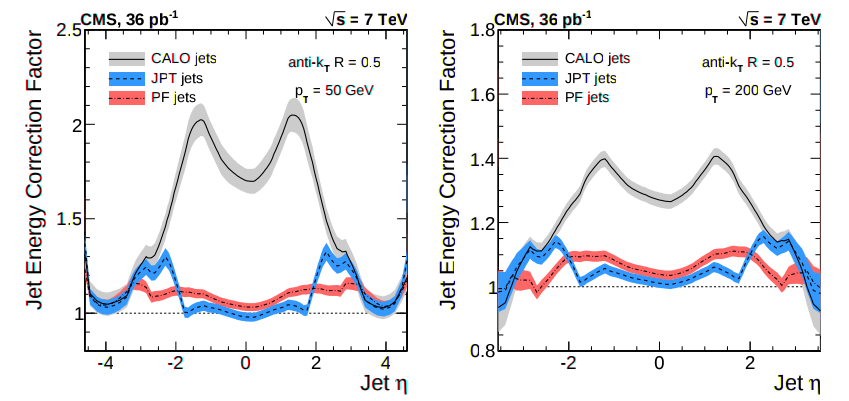
\includegraphics[width=1.2\largefigwidth]{plots/obj/jec.png}
  \DIFdelbeginFL %DIFDELCMD < \caption{%%%
\DIFdelendFL \DIFaddbeginFL \caption[Total jet-energy-correction factor as a function of jet $\eta$ for jets with $\pt=50$\GeV\, (left) and $\pt=200$\GeV\, (right), for several types of jet reconstruction used at CMS. The bands indicate the corresponding uncertainty.]{\DIFaddendFL Total jet-energy-correction factor as a function of jet $\eta$ for jets with $\pt=50$\GeV\, (left) and $\pt=200$\GeV\, (right), for several types of jet reconstruction used at CMS. The bands indicate the corresponding uncertainty~\cite{CMS-JME-10-011}.}
  \label{fig:jec}
\end{figure}
\section{Missing transverse energy}
\label{sec:MET}
%Describe MET reconstruction
Particles which interact only weakly with normal matter\DIFaddbegin \DIFadd{, }\DIFaddend such as neutrinos and hypothetical \ac{DM} particles\DIFaddbegin \DIFadd{, }\DIFaddend will pass through the CMS detector without interacting. The only signature that they leave is a momentum imbalance between the visible particles in an event. The \DIFaddbegin \DIFadd{initial transverse momentum of the colliding protons is low (less than a }\ac{GeV}\DIFadd{), so any significant imbalance can be interpreted as evidence for non-interacting particles. The }\DIFaddend high hermeticity of the CMS detector allows this imbalance, the \MET, first described in \SectionRef{sec:higprod}, to be measured accurately. As the analyses described in this thesis are searches for invisibly decaying Higgs bosons, the measurement of \MET is crucial.

%Algorithm
The CMS \MET reconstruction algorithm defines \DIFdelbegin \DIFdel{the }\DIFdelend \MET as the negative vectorial sum of the \pt of all \ac{PF} candidates~\cite{CMS-PAS-JME-12-002}. For processes such as \PZ boson decays to muon pairs\DIFaddbegin \DIFadd{, }\DIFaddend or $\gamma$+jets\DIFaddbegin \DIFadd{, }\DIFaddend there should be no \MET as all the decay products are visible. However, as can be seen from \FigureRef{fig:metresponse}, these events often still appear to have \MET due to the resolution of the \pt measurements of the various objects making up the \ac{PF} candidates, primarily the jets which are numerous and do not have as good resolution as other objects.

\begin{figure}
  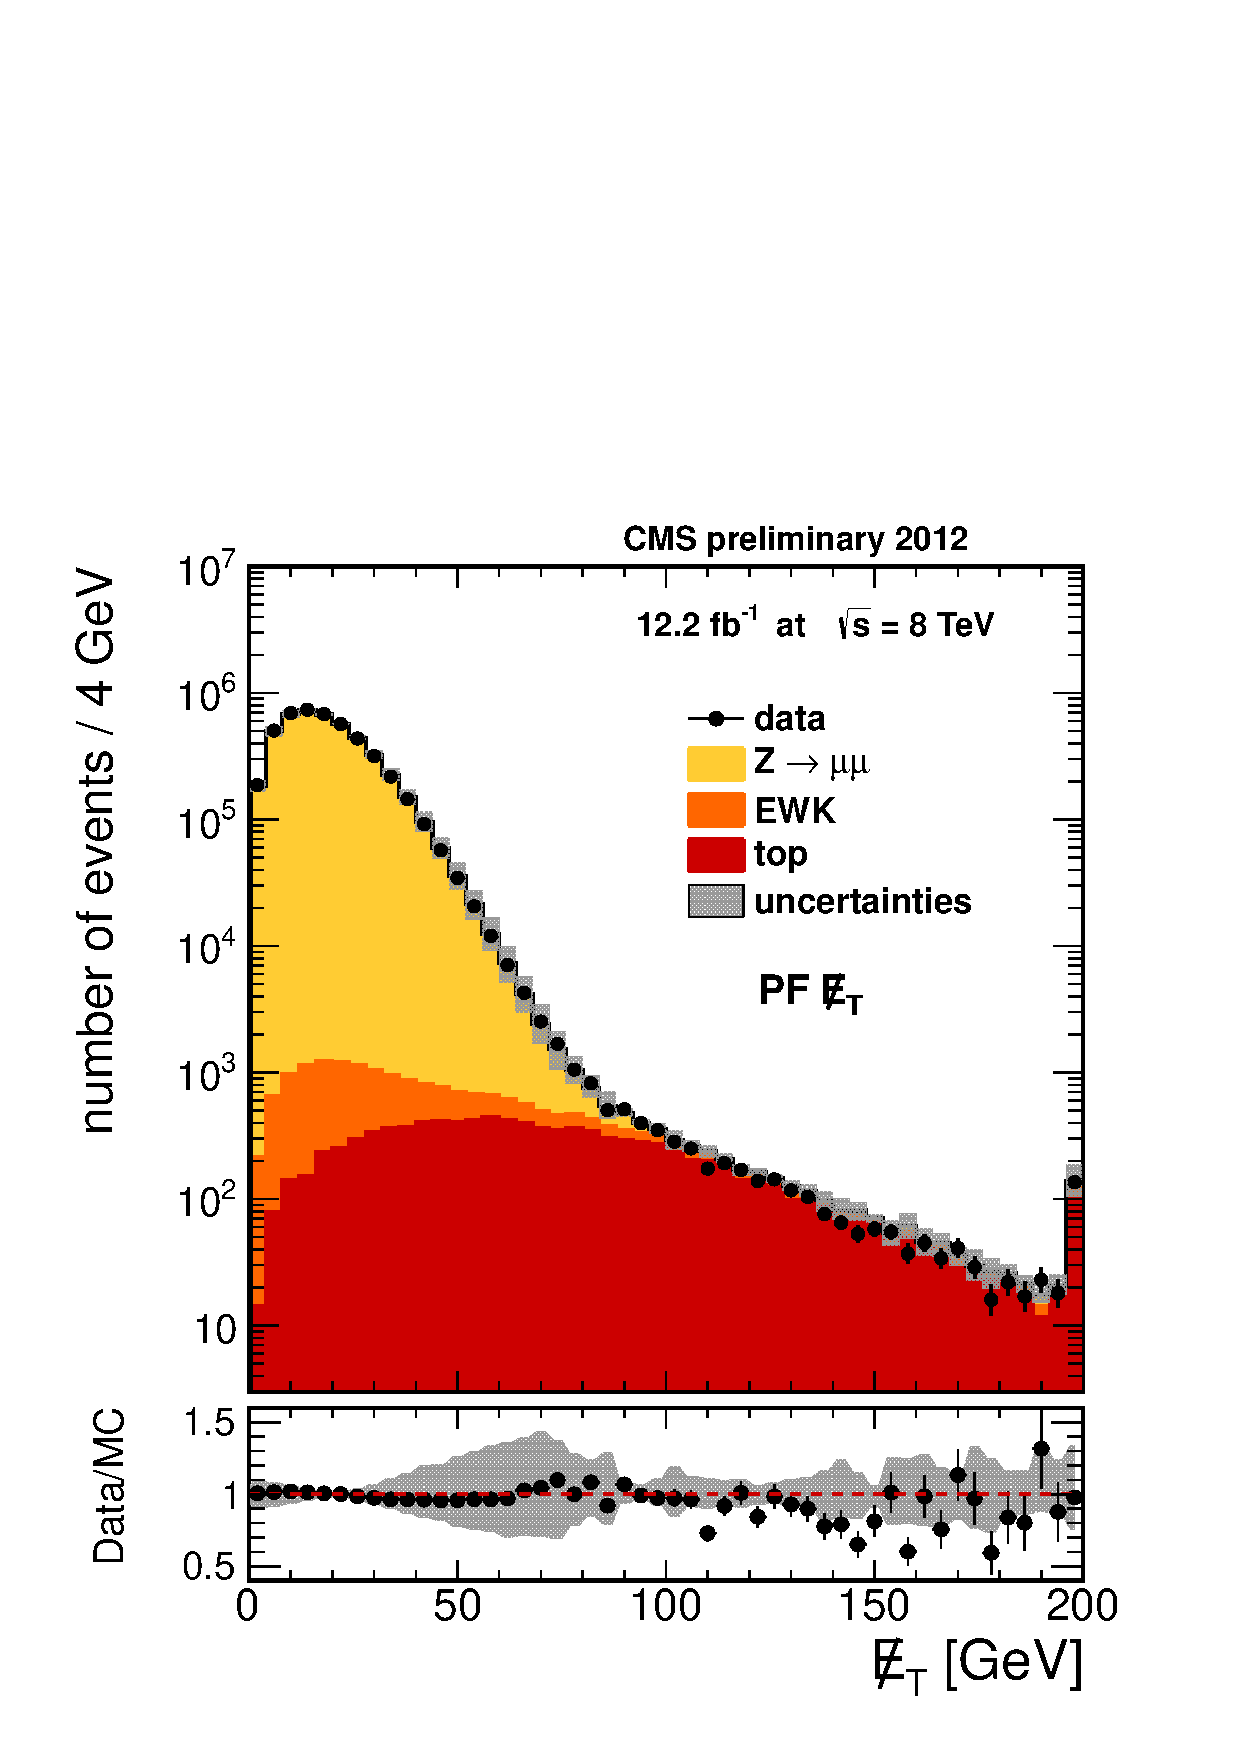
\includegraphics[width=0.6\largefigwidth]{plots/obj/metzmumu.pdf}
  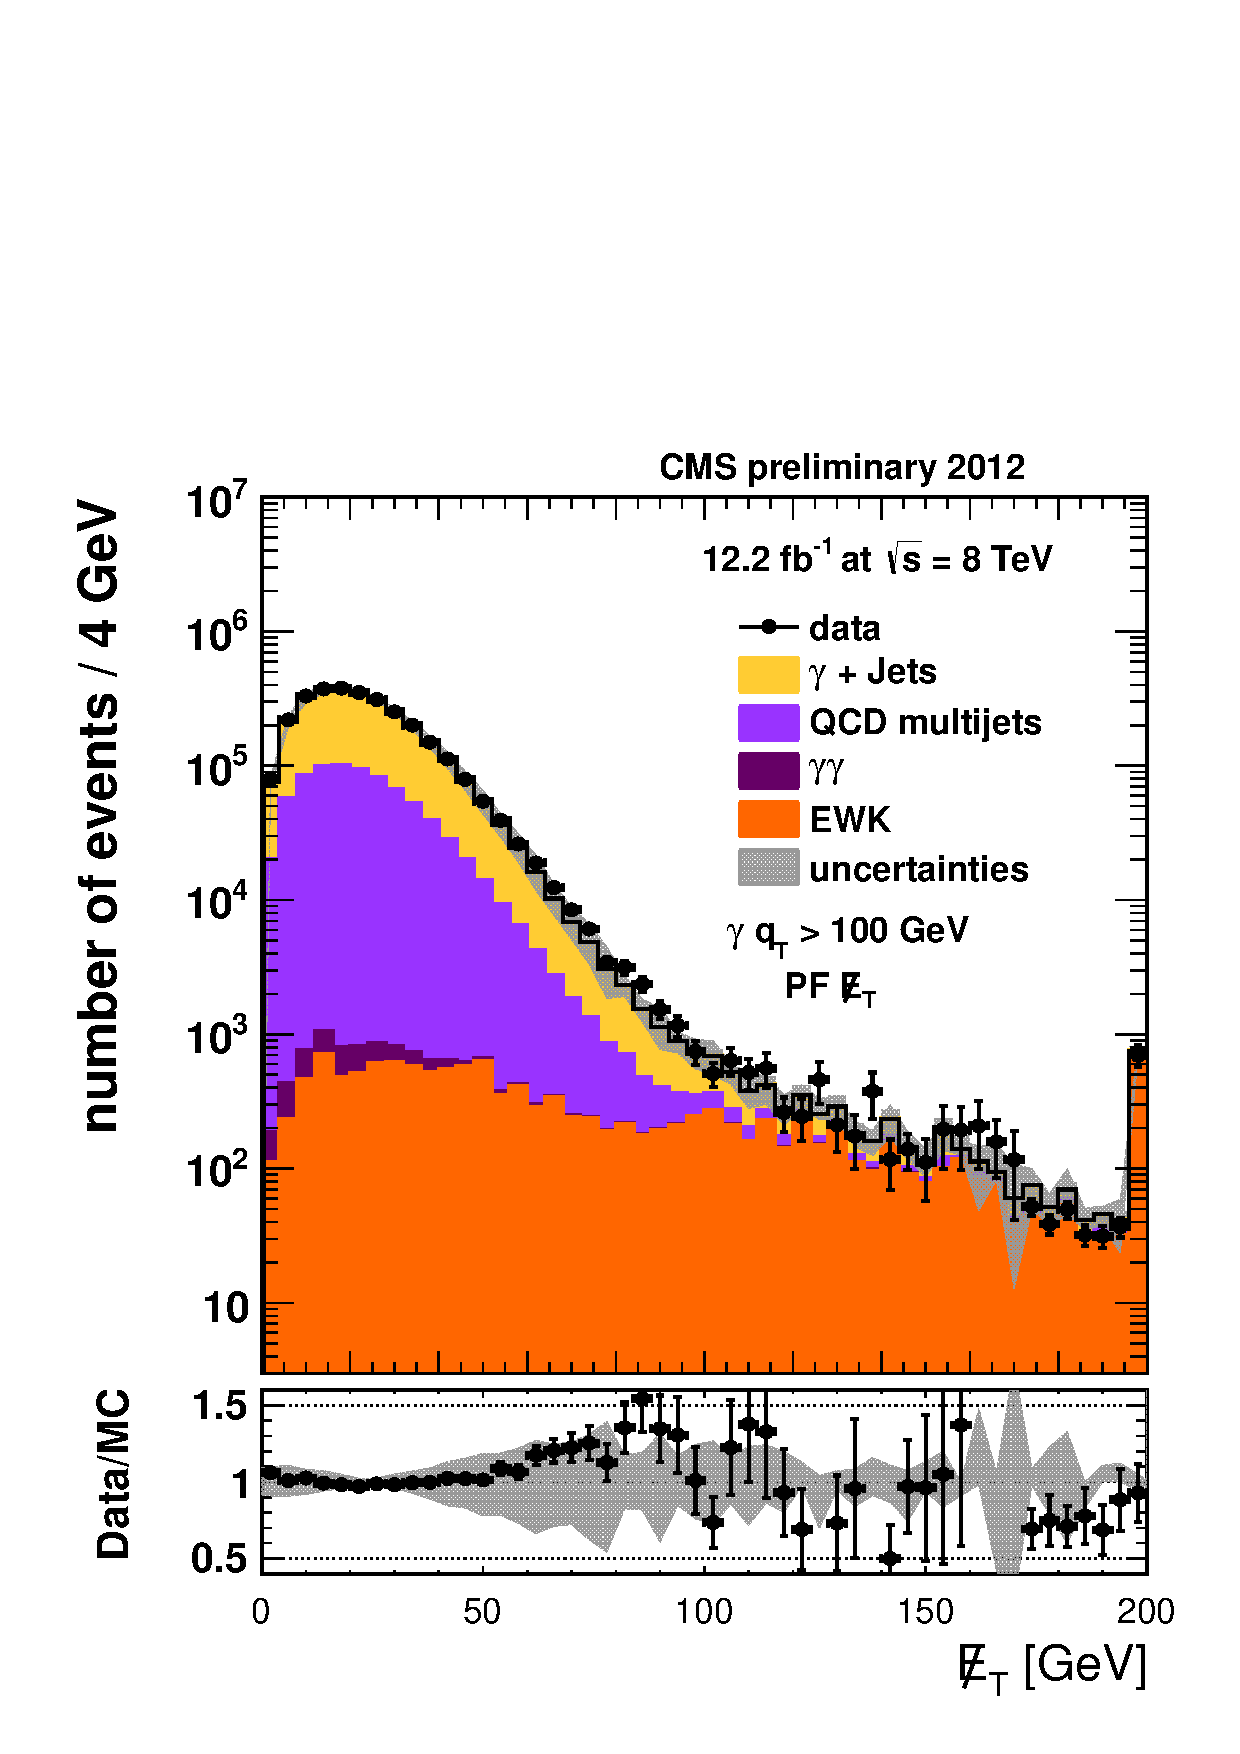
\includegraphics[width=0.6\largefigwidth]{plots/obj/metgammajets.pdf}
  \DIFdelbeginFL %DIFDELCMD < \caption{%%%
\DIFdelendFL \DIFaddbeginFL \caption[Distributions of the uncorrected \MET in $\PZ\rightarrow\mu\mu$ events (left) and $\gamma$+jets events (right) in $\sqrt{s}=8$\TeV\, data and simulation. The shaded band corresponds to the systematic uncertainty.]{\DIFaddendFL Distributions of the uncorrected \MET in $\PZ\rightarrow\mu\mu$ events (left) and $\gamma$+jets events (right) in $\sqrt{s}=8$\TeV\, data and simulation. The shaded band corresponds to the systematic uncertainty~\cite{CMS-PAS-JME-12-002}.}
  \label{fig:metresponse}
\end{figure}

The jet energy corrections, described in \SectionRef{sec:jec}, alter the energy of jets, and in doing so alter the total energy present in the event. These changes are propagated to the \MET. Furthermore, as charged particle flow candidates can be determined to be from the \ac{PV} or a \ac{PU} vertex it is also possible to correct the \MET for \ac{PU} contributions. This correction uses the ratio of the energy response of CMS for charged and neutral particles to estimate the neutral \ac{PU} contribution from the charged \ac{PU} contribution.

In addition to the above corrections, filters are applied to reject events where detector or beam effects lead to a high probability of spurious \MET. Examples of the effects which are removed with these filters include particles directly hitting the photodetectors in the \ac{ECAL} or significant energy deposits from the halo of particles surrounding the \LHC beam.

%METNOMU
In the \ac{VBF} invisible Higgs boson decay searches described below events with \PW or \PZ boson decays to muons are used to estimate the rate of some background processes. As part of this estimation the muons from the \PW or \PZ boson decays are ignored when calculating the \MET. The variable \METnoMU, which is the \MET calculated ignoring all tight muons, is used for this estimation.
\section{Taus}
\label{sec:taus}
%Describe tau reconstruction %Relevance to analysis
Approximately 35\% of taus decay to lighter charged leptons and neutrinos~\cite{pdg}. In this case, due to the short lifetime of the tau, the resulting charged leptons are reconstructed as prompt electrons or muons and the neutrinos cause \MET, therefore no specific tau reconstruction is necessary. However, the other $\sim$65\% of tau decays are so-called hadronic tau decays, where the decay products are hadrons and a tau neutrino. This section will describe the reconstruction of these tau decays.

%Algorithm
CMS uses \DIFdelbegin \DIFdel{a }\DIFdelend \DIFaddbegin \DIFadd{the so-called }\DIFaddend \ac{HPS} algorithm for reconstructing hadronic tau decays, described in detail in \ReferenceRef{CMS-PAS-TAU-11-001}. Almost all hadronic tau decay modes consist of one or three charged hadrons and up to two neutral pions~\cite{pdg}. The \ac{HPS} algorithm aims to reconstruct both the charged hadrons and the photons which result from the neutral pion decays.

The \ac{HPS} algorithm is seeded by a \ac{PF} jet, described in \SectionRef{sec:jets}, and starts by creating a \DIFdelbegin \DIFdel{strip }\DIFdelend \DIFaddbegin \DIFadd{``strip'' }\DIFaddend with the four-momentum of the most energetic \ac{EM} \ac{PF} candidate, i.e. photon or electron, in the jet. Other \ac{EM} candidates are then searched for within  a window of 0.05 (0.2) in $\eta$ ($\phi$) of the strip's centre. The most energetic particle that is found is added to the strip and the four-momentum is updated. This process is repeated until no more particles are found, and if the strip has \pt$>1$\GeV\, at this point it is kept. Combinations of charged hadrons and strips consistent with tau decay modes are then searched for, and if one is found the resulting combination is taken to be a hadronic tau.

Taus are required to be isolated. The isolation is calculated as the sum of all hadronic and photon \ac{PF} candidates from the \ac{PV} within a cone of size $\Delta R=0.5$ of the tau. \ac{PF} candidates not compatible with the \ac{PV} within 0.8 in $R$ of the tau are used to estimate and correct for the contribution to the isolation from \ac{PU}. 

Electrons which emit Bremsstrahlung photons can look very much like one charged hadron plus a neutral pion. A \ac{BDT} is trained, using similar variables to those used for the electron identification in \SectionRef{sec:electrons}, to remove these particles. Taus that are consistent with being from a muon are also rejected. This rejection is performed by requiring that the tau is not reconstructed as a track compatible with hits in the muon system. The final efficiency of the CMS hadronic tau reconstruction for taus with \pt$>20$ \GeV is found to be 55\%, with a fake rate of 2 (3)\% for non-hadronic tau objects to be reconstructed as hadronic taus in the barrel (endcap) region of the detector.

\section{MC weights}
\label{sec:mcweights}
As discussed in \SectionRef{sec:sim} proton-proton collisions at the \LHC are simulated using \ac{MC} generators. In some cases the results of these simulations need to be modified to better match the observed data, by ``weighting'' the \ac{MC} events. One example of this is cross-section weighting, where a weight is applied to account for the difference between the number of events generated and that expected to be observed in data for a given integrated luminosity. Further weights are applied to correct the generated distribution of the number of primary vertices to match that in data (called pileup reweighting), to account for differences between the simulated lepton identification efficiency and that observed in data, and to correct the generated \pt spectrum of top quarks to better match that observed in data.
\chapter{Search for invisibly decaying VBF produced Higgs bosons in Run 1 prompt data}
\label{chap:prompt}
%Introduction to selection and challenges of jets+met, e.g. trigger, \ac{QCD}
As described in \ChapterRef{chap:theory}, searches for invisible Higgs boson decays are well motivated by their sensitivity to new physics, such as \ac{DM}. Because \BRinv of an \ac{SM} 125 \GeV Higgs boson is very small, any evidence for invisible Higgs boson decays at the \LHC would be evidence for physics beyond the \ac{SM}. This chapter describes the search for invisible Higgs boson decays using data taken by CMS in 2012 which was promptly reconstructed. A dedicated trigger was developed specifically for this analysis. The total integrated luminosity collected with this trigger that was certified for use in physics analyses was 19.5\DIFaddbegin \,\DIFaddend \invfb~\cite{CMS-PAS-LUM-13-001}. The analysis was published in \ReferenceRef{Chatrchyan:2014tja}.

\section{Event selection}
\label{sec:promptsel}
%describe backgrounds and motivate selection
Signal events are expected to have two jets with a characteristic \ac{VBF} topology and a large amount of \MET. Several background processes, with significantly higher cross-sections than the signal process, can also produce events containing these objects. It is therefore necessary to design selection criteria, known as ``cuts'', to remove as many of these background events from the analysis as possible, whilst retaining the maximum number of signal events.

The most significant of these background processes is the production of a vector boson in association with jets, ``V+jets''. Leptonic decays of \PW bosons and \PZ boson decays to neutrinos both produce \MET and, due to the approximately 1000 times higher cross-section for vector boson production than Higgs boson production, in many events the associated jets have a \ac{VBF}-like topology~\cite{CMSSMPPublic}. V+jets backgrounds with a \PW (\PZ) are referred to as ``\PW(\PZ)+jets''.
A further background process that can produce significant numbers of \ac{VBF}-like jets due to its very large cross-section is \ac{QCD} production of multiple jets (``\ac{QCD} multijets'' or simply ``\ac{QCD}''). Whilst these multijet events have very little \MET from real invisible particles, it is possible for significant ``fake'' \MET to be caused by mismeasurement of the jets. The production of two vector bosons or top quarks can also lead to two jets and real \MET, although they have much lower cross-sections than the other background processes and their contribution is not as significant. %relative cross-section

%trigger requirements and design
\subsection{Trigger}
\label{sec:prompttrig}
The trigger requirements can be viewed as the first stage of the event selection. Their primary role is to reduce the rate of events that must be recorded by the detector, whilst retaining the maximum number of signal events. As described in \SectionRef{sec:triggers}, the decision whether to keep an event must be made very rapidly and, as a result, the object reconstruction algorithms used are less sophisticated, and the granularity of the information available from the CMS subdetectors is worse than those offline. The trigger criteria have therefore been chosen to be as loose as possible whilst achieving the required rate reduction.

As it is the key variable which indicates the presence of invisible particles, all events passing the trigger are required to have significant \MET. To pass the \ac{L1} trigger selection events are required to have \MET$>40$ \GeV. The \ac{HLT} selection also requires that events have \METnoMU$>65$\GeV. The use of \METnoMU at trigger level ensures that events that are needed for the control regions used in the background estimation techniques described in \SectionRef{sec:promptbkg} are not rejected. In addition to this \METnoMU requirement events must have at least one pair of jets \DIFdelbegin \DIFdel{in the event }\DIFdelend which is \ac{VBF}-like to pass the \ac{HLT} selection. The \ac{VBF}-like requirements on the jets consist of requiring their $\eta$ separation, \detajj, \DIFaddbegin \DIFadd{to }\DIFaddend be greater than 3.5, that they are in opposite forward/backward halves of the detector and that they have high invariant mass, $\Mjj>800 \GeV$. All of these jet requirements are motivated by the lack of colour connection between \DIFaddbegin \DIFadd{the jets in }\DIFaddend \ac{VBF} events leading to large angular separations between the two jets, as described in \SectionRef{sec:higprod}. \DIFaddbegin \DIFadd{The requirement that jets be in opposite forward/backward halves of the detector is made almost redundant by the }\detajj \DIFadd{cut, however it is a fast requirement to compute and is applied early in the list of trigger requirements and thus decreases the resource usage of the trigger. }\DIFaddend Not requiring that the \ac{VBF}-like pair of jets also be the two highest \pt jets reduces inefficiencies caused by different \pt orderings in jets reconstructed by the trigger and by the offline reconstruction.

The efficiency for events passing both the prompt analysis trigger and the two triggers used for the parked data analysis, described in \ChapterRef{chap:parked} as a function of their values of several offline variables, measured in single muon data collected using an uncorrelated trigger, is shown in Figs.~\ref{fig:prompttrigplots} and \ref{fig:prompttrigplots2}. The events used in the trigger efficiency measurement are required to pass the following cuts:
\begin{equation}
  \label{eq:prompttrigstudycuts}
  \Mjj>1100 \GeV, \METnoMU>130 \GeV, \mathrm{leading\,2\,jets'\,} \pt>50 \GeV, \detajj>4.2,\eta_{j1}\cdot\eta_{j2}<0.
\end{equation}
In each measurement the cut on the variable being studied is removed. The measured trigger efficiency is applied as an event-by-event weight to all \ac{MC} samples.

%trigger efficiency plots from trigeff310314
\begin{figure}
  \subfloat[]{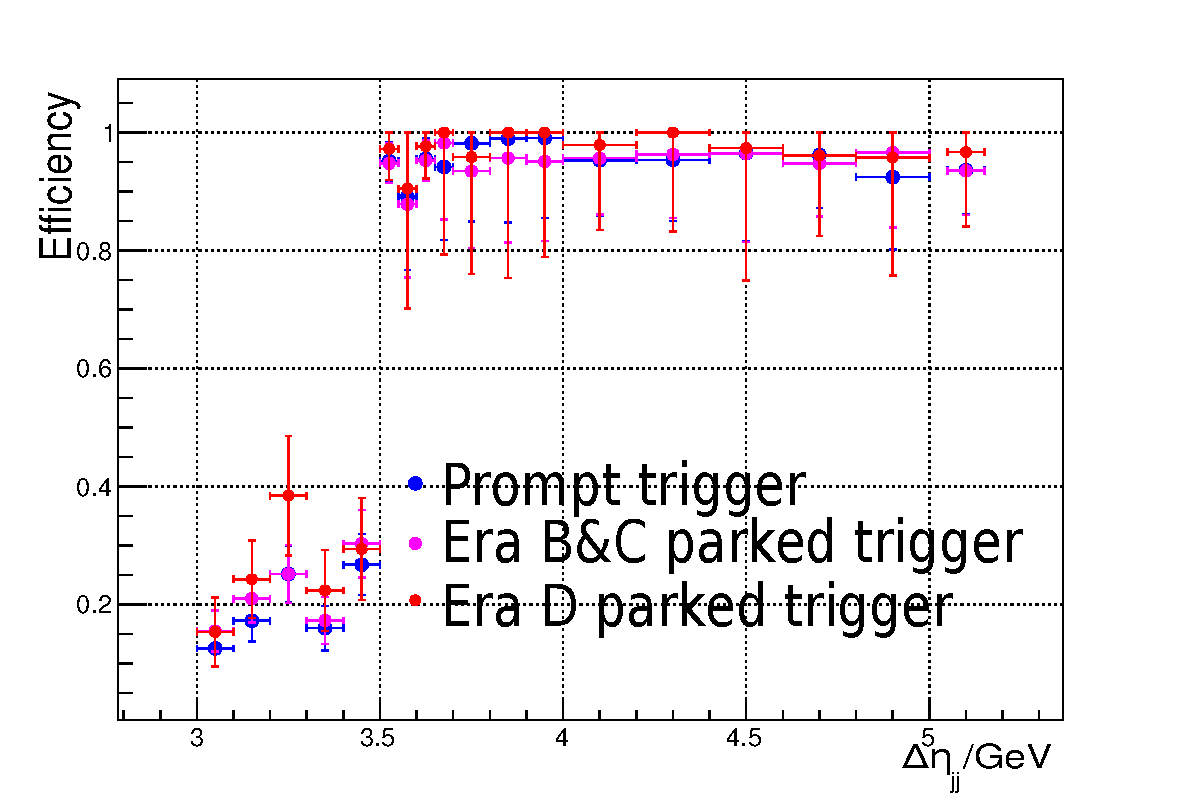
\includegraphics[width=.65\largefigwidth]{plots/prompt/trigeffplots_hltonly/detaefficiency.pdf}}
  \subfloat[]{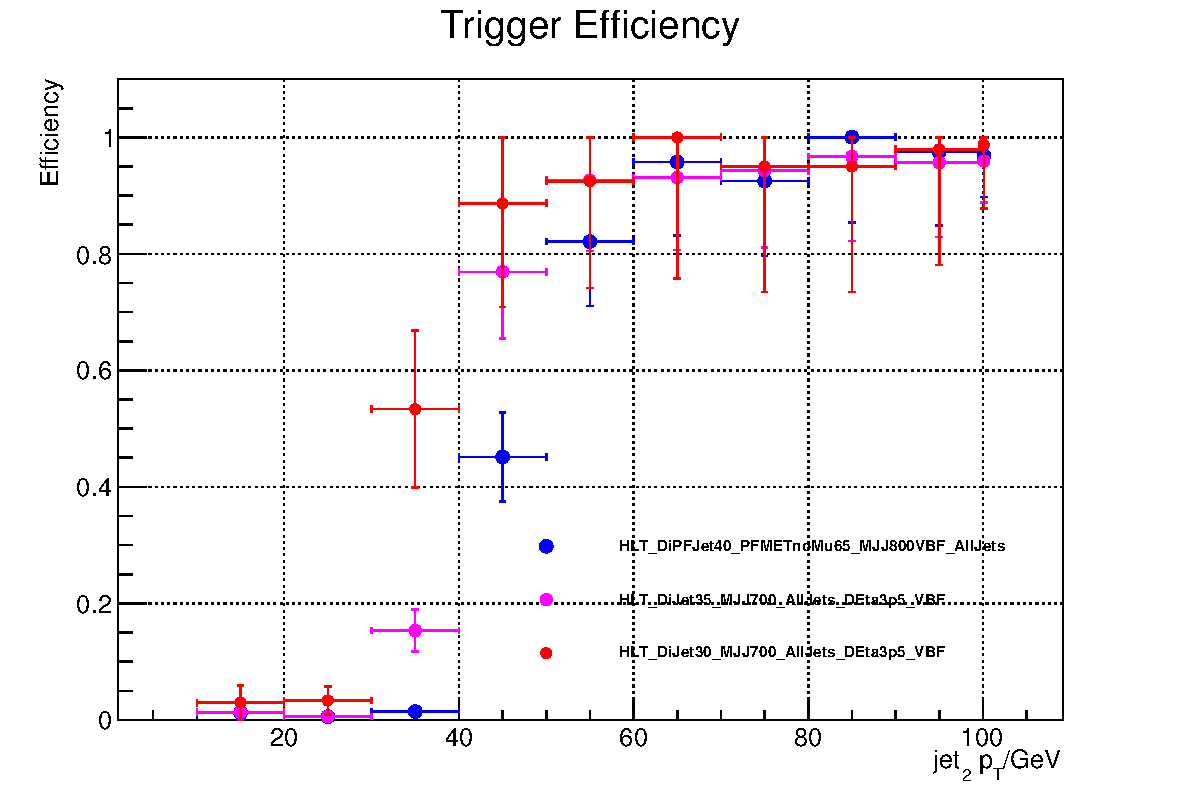
\includegraphics[width=.65\largefigwidth]{plots/prompt/trigeffplots_hltonly/j2ptefficiency.pdf}}

  \subfloat[]{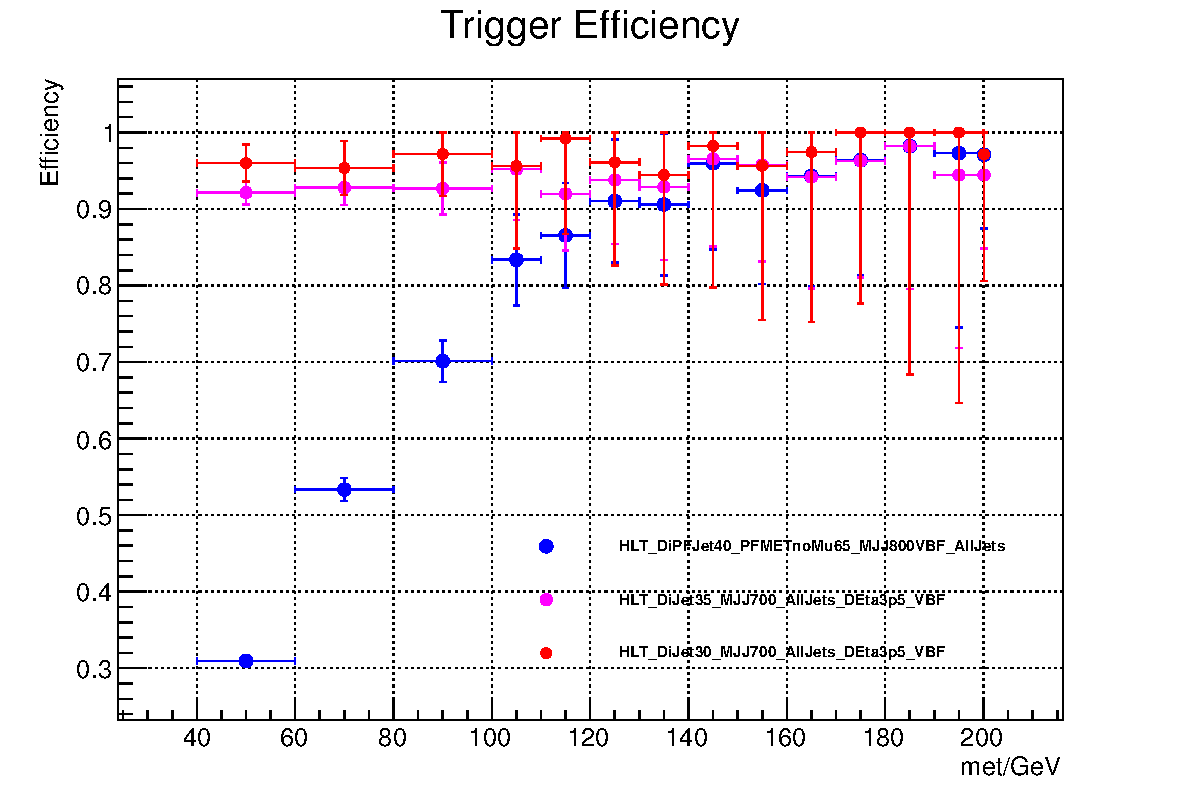
\includegraphics[width=.65\largefigwidth]{plots/prompt/trigeffplots_hltonly/metefficiency.pdf}}
  \subfloat[]{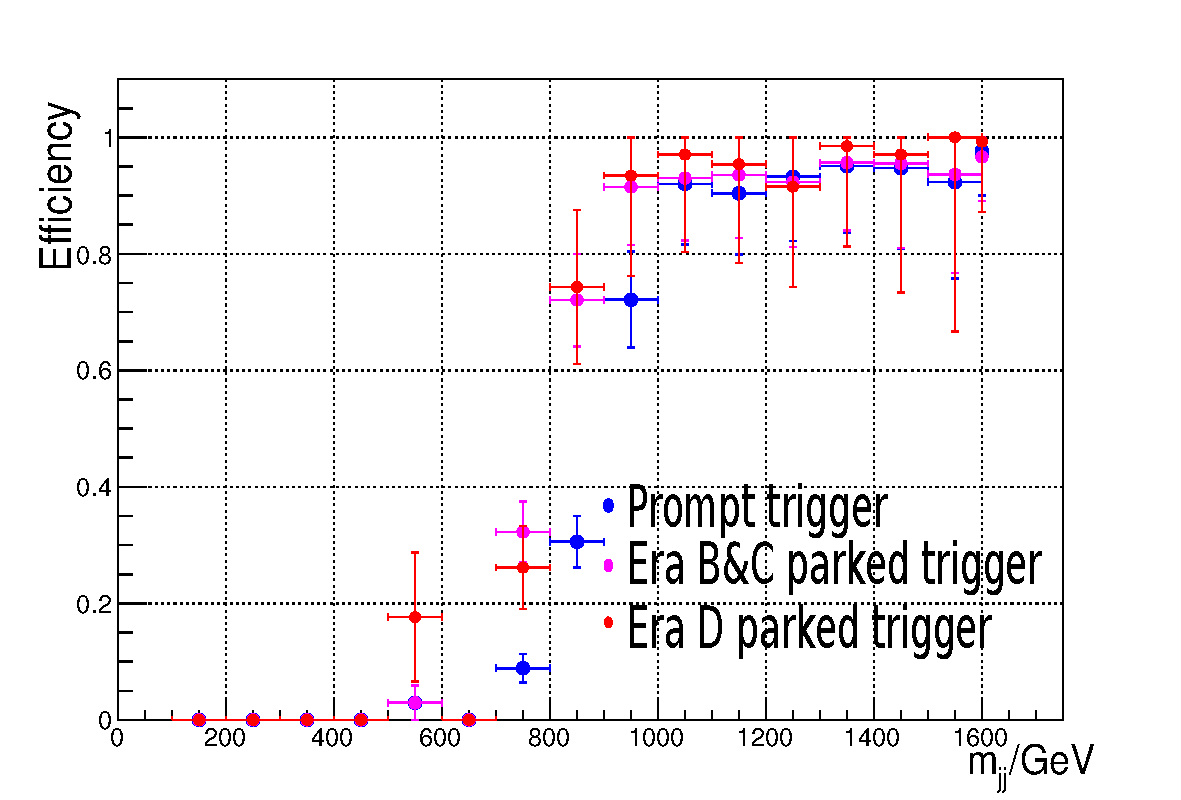
\includegraphics[width=.65\largefigwidth]{plots/prompt/trigeffplots_hltonly/mjjefficiency.pdf}}
  \caption{The efficiency of the \DIFdelbeginFL %DIFDELCMD < \ac{HLT} %%%
\DIFdelendFL \DIFaddbeginFL \DIFaddFL{HLT }\DIFaddendFL requirements used in the prompt (blue) and parked (purple and red) data analyses as a function of the values of several offline variables, measured in a sample of events recorded on a single-muon trigger. (a) Efficiency as a function of offline \detajj, (b) efficiency as a function of sub-leading jet \pt, (c) efficiency as a function of offline \METnoMU, (d) efficiency as a function of \Mjj.}
  \label{fig:prompttrigplots}
\end{figure}

\begin{figure}
  \subfloat[]{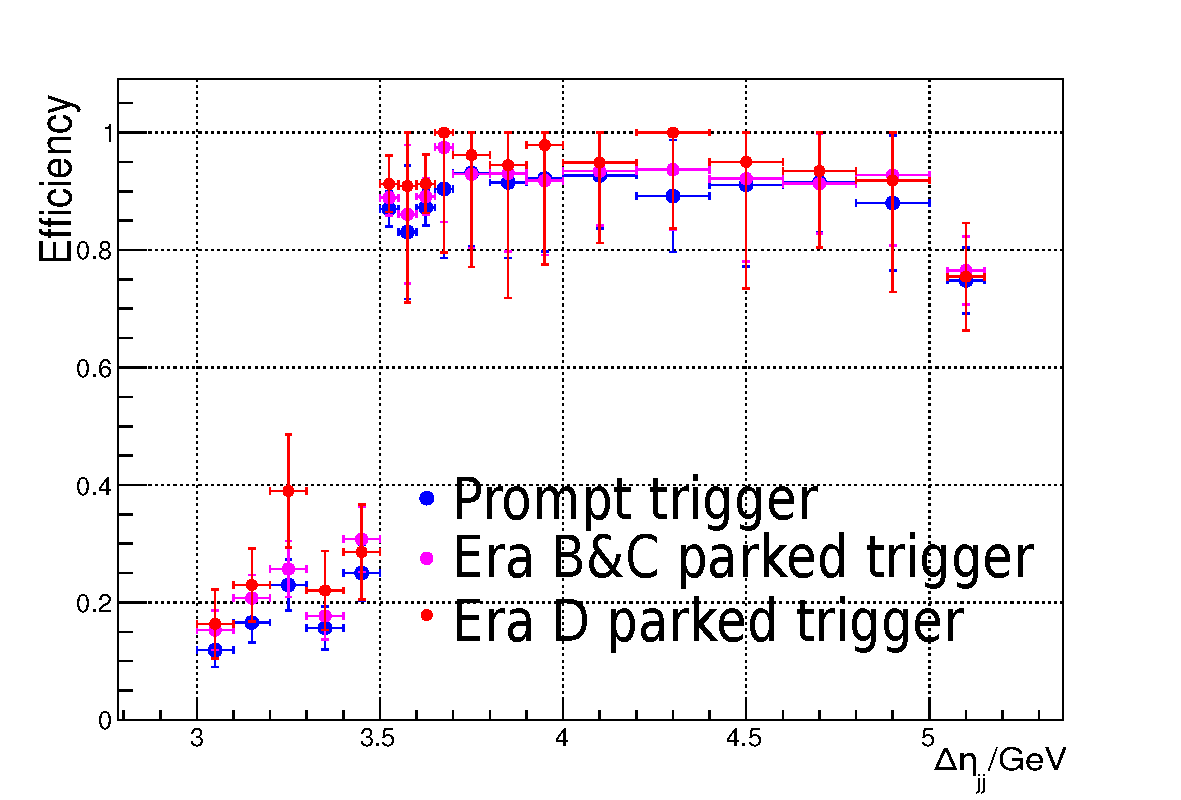
\includegraphics[width=.65\largefigwidth]{plots/prompt/trigeffplots_nol1cut/detaefficiency.pdf}}
  \subfloat[]{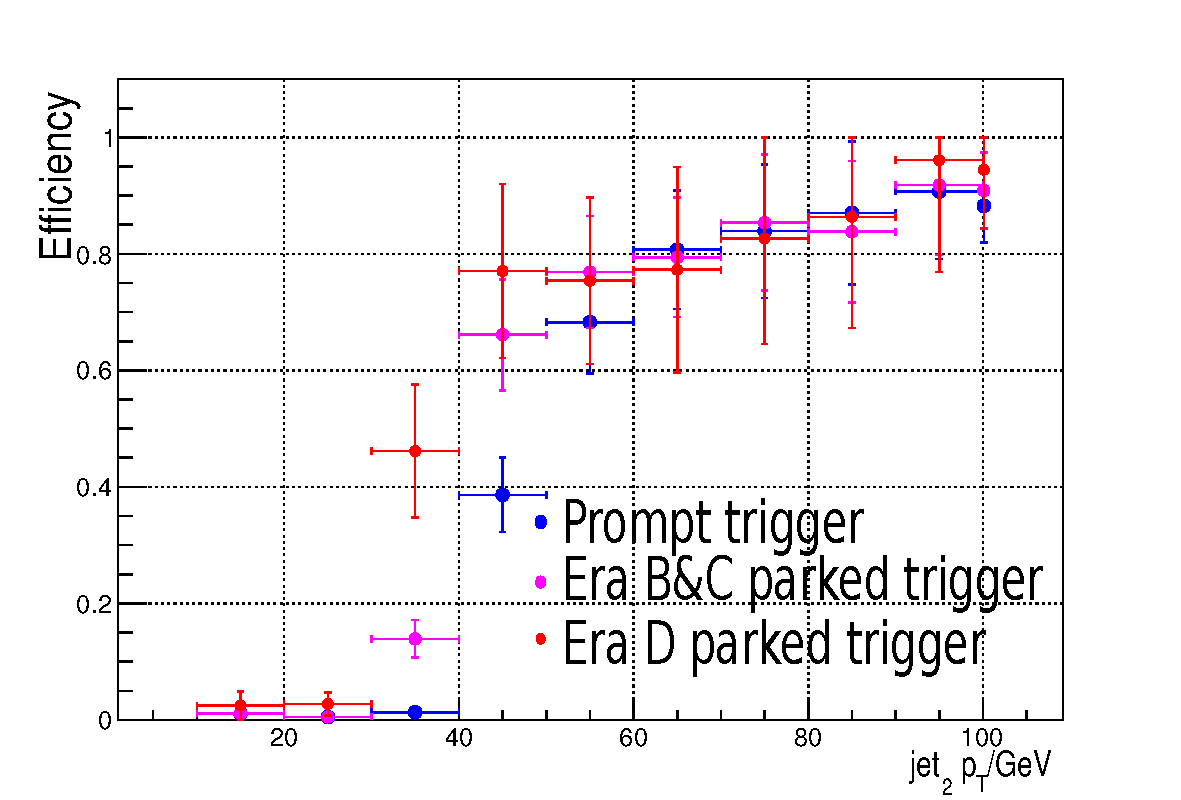
\includegraphics[width=.65\largefigwidth]{plots/prompt/trigeffplots_nol1cut/j2ptefficiency.pdf}}

  \subfloat[]{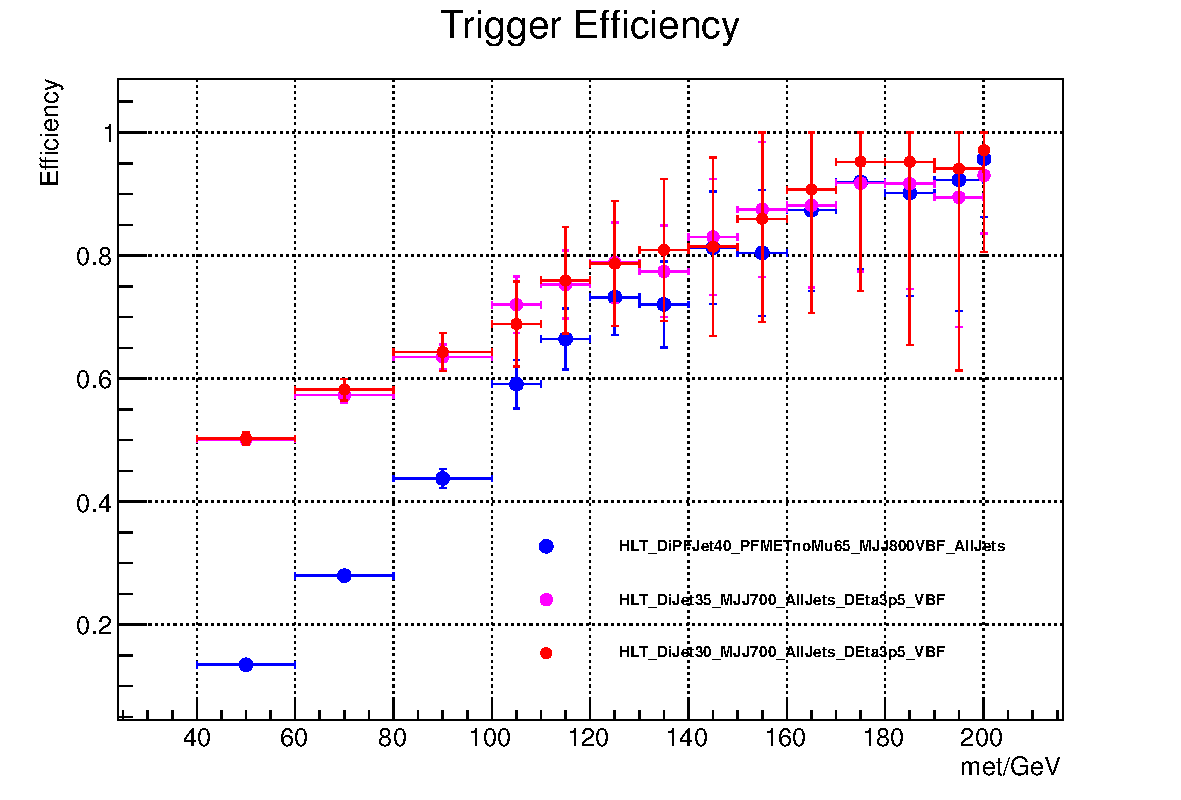
\includegraphics[width=.65\largefigwidth]{plots/prompt/trigeffplots_nol1cut/metefficiency.pdf}}
  \subfloat[]{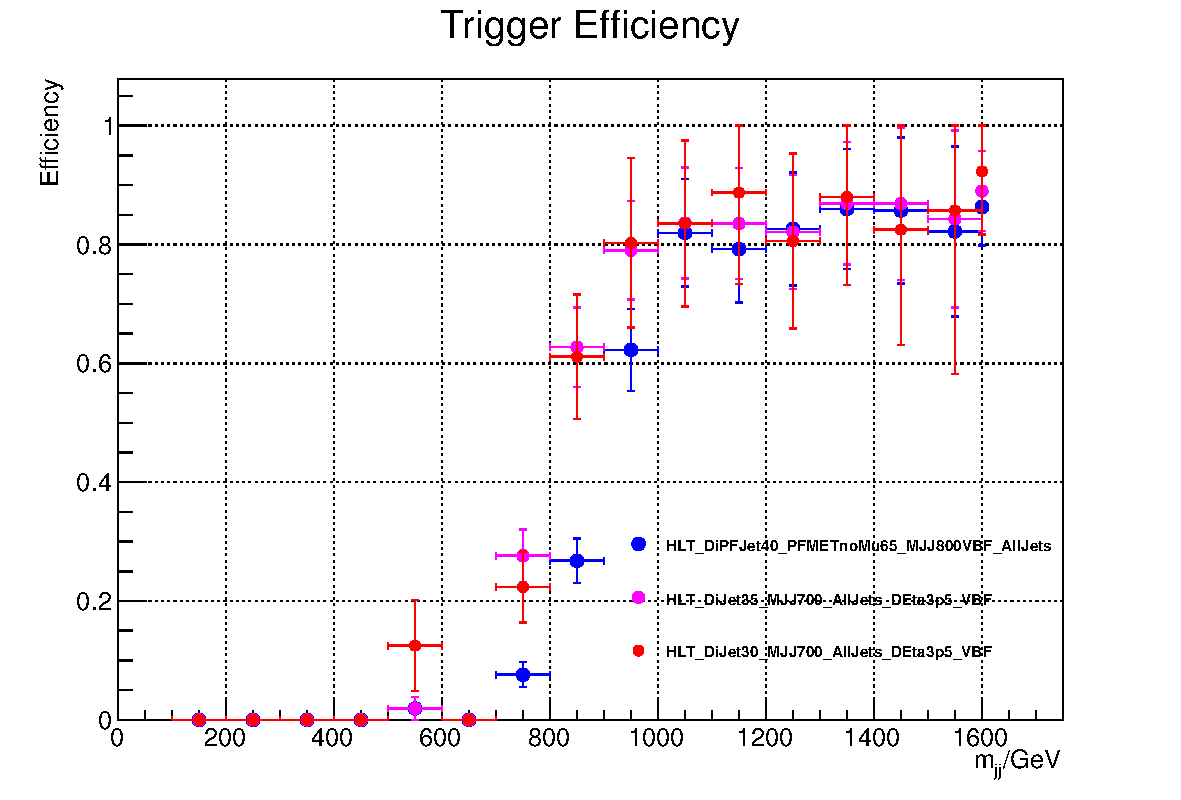
\includegraphics[width=.65\largefigwidth]{plots/prompt/trigeffplots_nol1cut/mjjefficiency.pdf}}
  \caption{The combined efficiency of the \DIFdelbeginFL %DIFDELCMD < \ac{HLT} %%%
\DIFdelendFL \DIFaddbeginFL \DIFaddFL{HLT }\DIFaddendFL and \DIFdelbeginFL %DIFDELCMD < \ac{L1} %%%
\DIFdelendFL \DIFaddbeginFL \DIFaddFL{L1 }\DIFaddendFL trigger requirements used in the prompt (blue) and parked (purple and red) data analyses as a function of the values of several offline variables, measured in a sample of events recorded on a single-muon trigger. (a) Efficiency as a function of offline \detajj, (b) efficiency as a function of sub-leading jet \pt, (c) efficiency as a function of offline \METnoMU, (d) efficiency as a function of \Mjj.}
  \label{fig:prompttrigplots2}
\end{figure}

\subsection{Offline selection}
\label{sec:promptofflinesel}
%selection and motivation
The offline selection is chosen for three reasons. Firstly, the reconstruction algorithms for some objects are only well validated for certain values of \pt and $\eta$. This consideration decides the $\pt$ thresholds for jets and leptons to be used. Secondly, as can be seen from \FigureRef{fig:prompttrigplots}, the values of the offline variables where the trigger becomes fully efficient are in some cases much higher than the online cut. Because the variables used in the trigger are highly correlated, and the measurements of trigger efficiency made do not take this into account, the offline cuts on all variables used in the trigger were chosen such that the trigger efficiency for the variable at that point is greater than 95\%. Finally, some of the cuts imposed aim to reduce the contribution from background processes, which improves the signal to background ratio in the resulting region, and thus the expected limit on \BRinv.

The specific set of offline selection cuts chosen begins by requiring that events have no veto muons or electrons, as defined in \DIFdelbegin \DIFdel{sections }\DIFdelend \DIFaddbegin \DIFadd{Sections }\DIFaddend \ref{sec:electrons} and \ref{sec:muons}. Signal events are not expected to contain leptons, while background events are, so this lepton veto reduces the background from \PW and \PZ boson decays and also from top quarks without removing signal events. The two highest \pt jets in the event are then identified as the VBF tag pair, and tighter versions of the trigger selection, motivated by the trigger efficiency considerations described above, are then applied. Specifically, the tag jets are required to be in opposite forward/backward halves of the detector, to both have \pt$>50$ \GeV to have $\Mjj>1100$ \GeV and $\detajj>4.2$. Again due to trigger efficiency considerations, \METnoMU is required to be greater than 130 \GeV.  Because events with veto muons have been removed by the lepton veto, \METnoMU in this region is identical to \MET. However, it is important for background estimation methods that \METnoMU and not \MET is used.

As well as the \DIFdelbegin \DIFdel{trigger based }\DIFdelend \DIFaddbegin \DIFadd{trigger-based }\DIFaddend selection, further cuts are made to reduce the \ac{QCD} background to a level much lower than the V+jets backgrounds. The two tag jets are required to have an azimuthal separation, $\dphijj<1.0$, since multijet events with \MET due to mismeasurement are most likely to have their jets back-to-back in the detector, i.e. with $\dphijj=\pi$. Events where there are any jets with \pt$>30$ \GeV between the two tag jets in $\eta$ are also vetoed. This \ac{CJV} is motivated by the lack of colour connection, described in \SectionRef{sec:higprod}, between the quarks in VBF production that makes the presence of such jets unlikely in genuine signal events. The region of phase space remaining after all these cuts have been applied is called the signal region.

Finally, the values of the cuts are optimised to provide the best expected limit on \BRinv\, for a 125 \GeV Higgs boson, which is calculated using the method described in \SectionRef{sec:stats} using the same background estimation and systematic uncertainties as the final analysis \DIFaddbegin \DIFadd{(}\DIFaddend as described in Sections~\ref{sec:promptbkg} and \ref{sec:promptsyst} respectively\DIFaddbegin \DIFadd{)}\DIFaddend . For the tag jet \pt and \METnoMU, no improvement in the expected limit is seen by tightening the cut, so the requirement is set at the 95\% efficiency point of the trigger. The distributions and cut values for several of the other variables used are shown in \FigureRef{fig:promptcontrolplots}. The full selection gives an efficiency of $(6.8\pm 0.3)\times 10^{-3}$ for selecting events from invisible decays of a \DIFdelbegin \DIFdel{VBF produced }\DIFdelend \DIFaddbegin \DIFadd{VBF-produced }\DIFaddend 125 \GeV Higgs boson, measured using \ac{MC}.  

%discriminating variable plots from HIG-13-030
\begin{figure}
  \subfloat[]{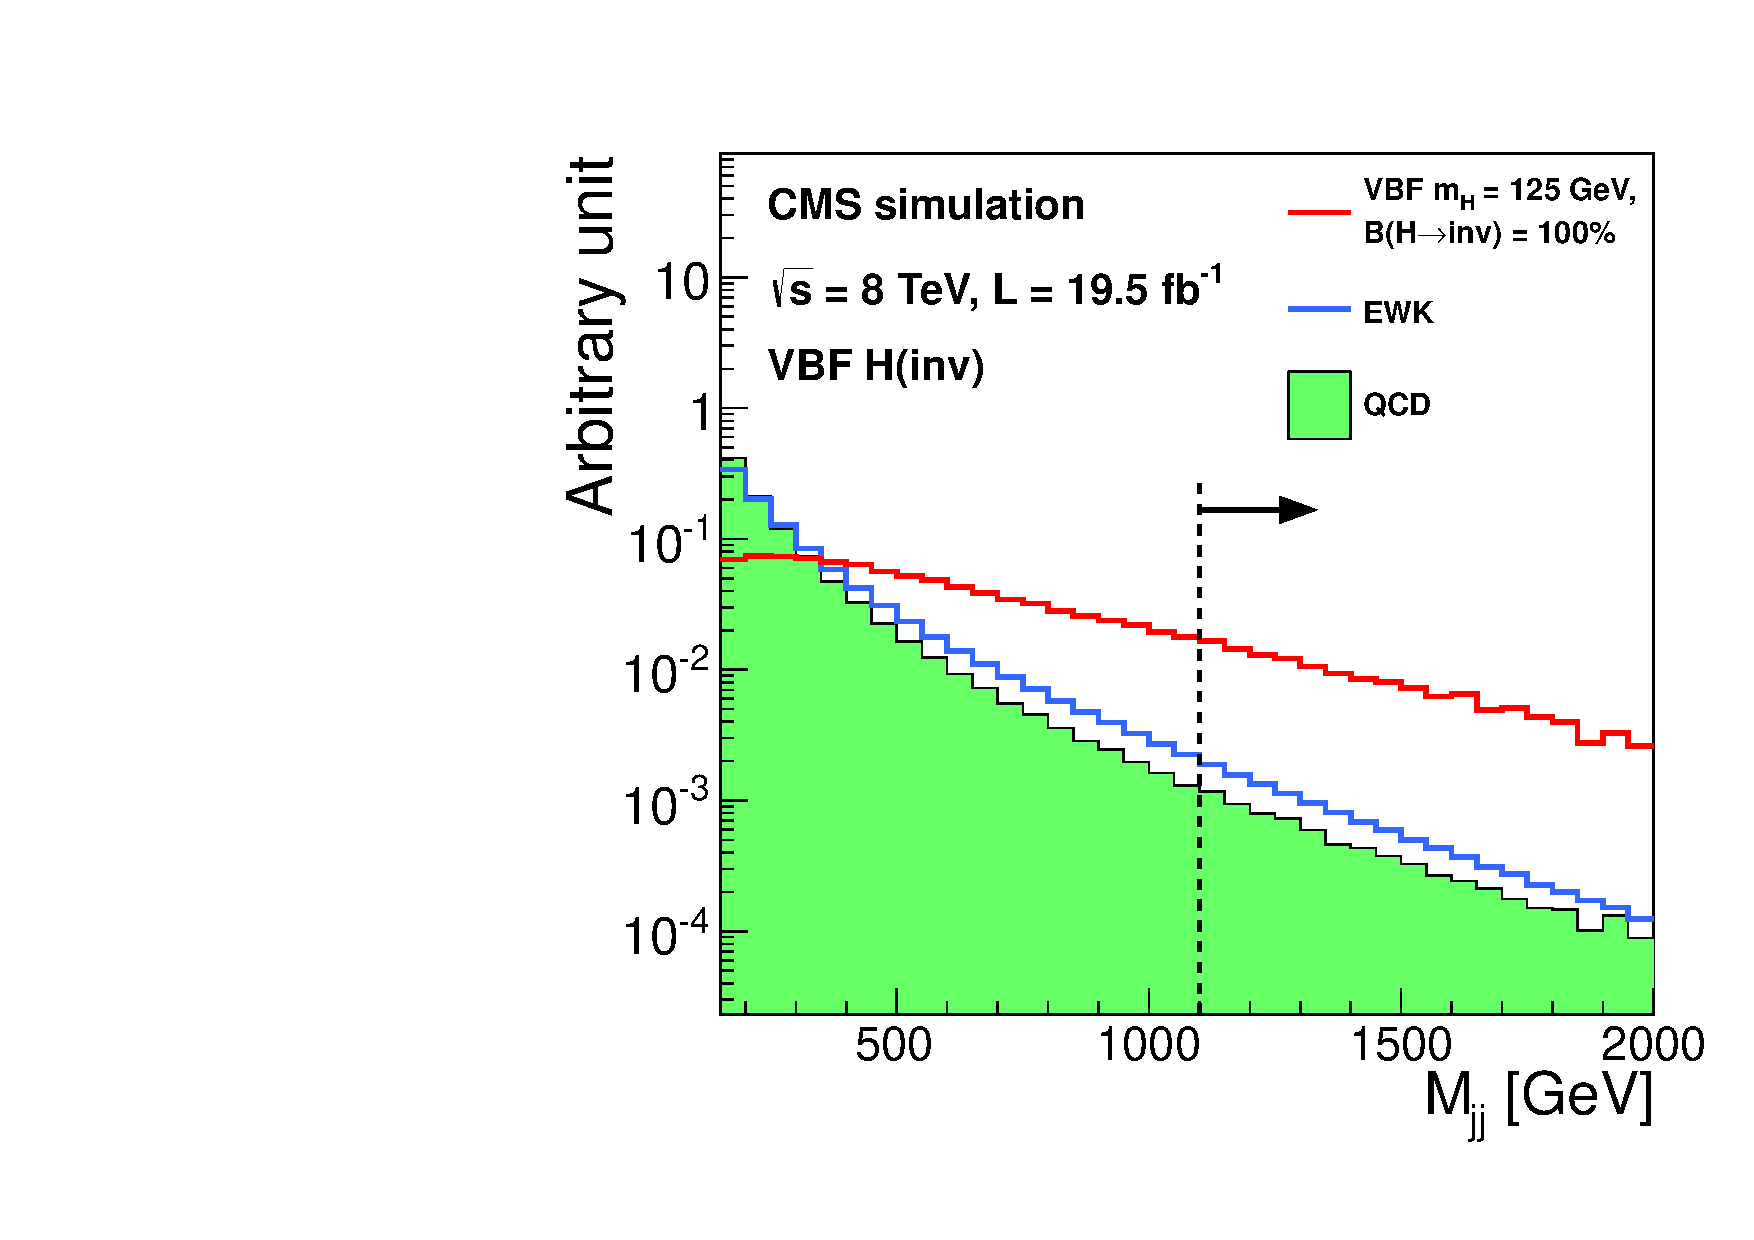
\includegraphics[width=.65\largefigwidth]{plots/prompt/VBF-Dijet-M.pdf}}
  \subfloat[]{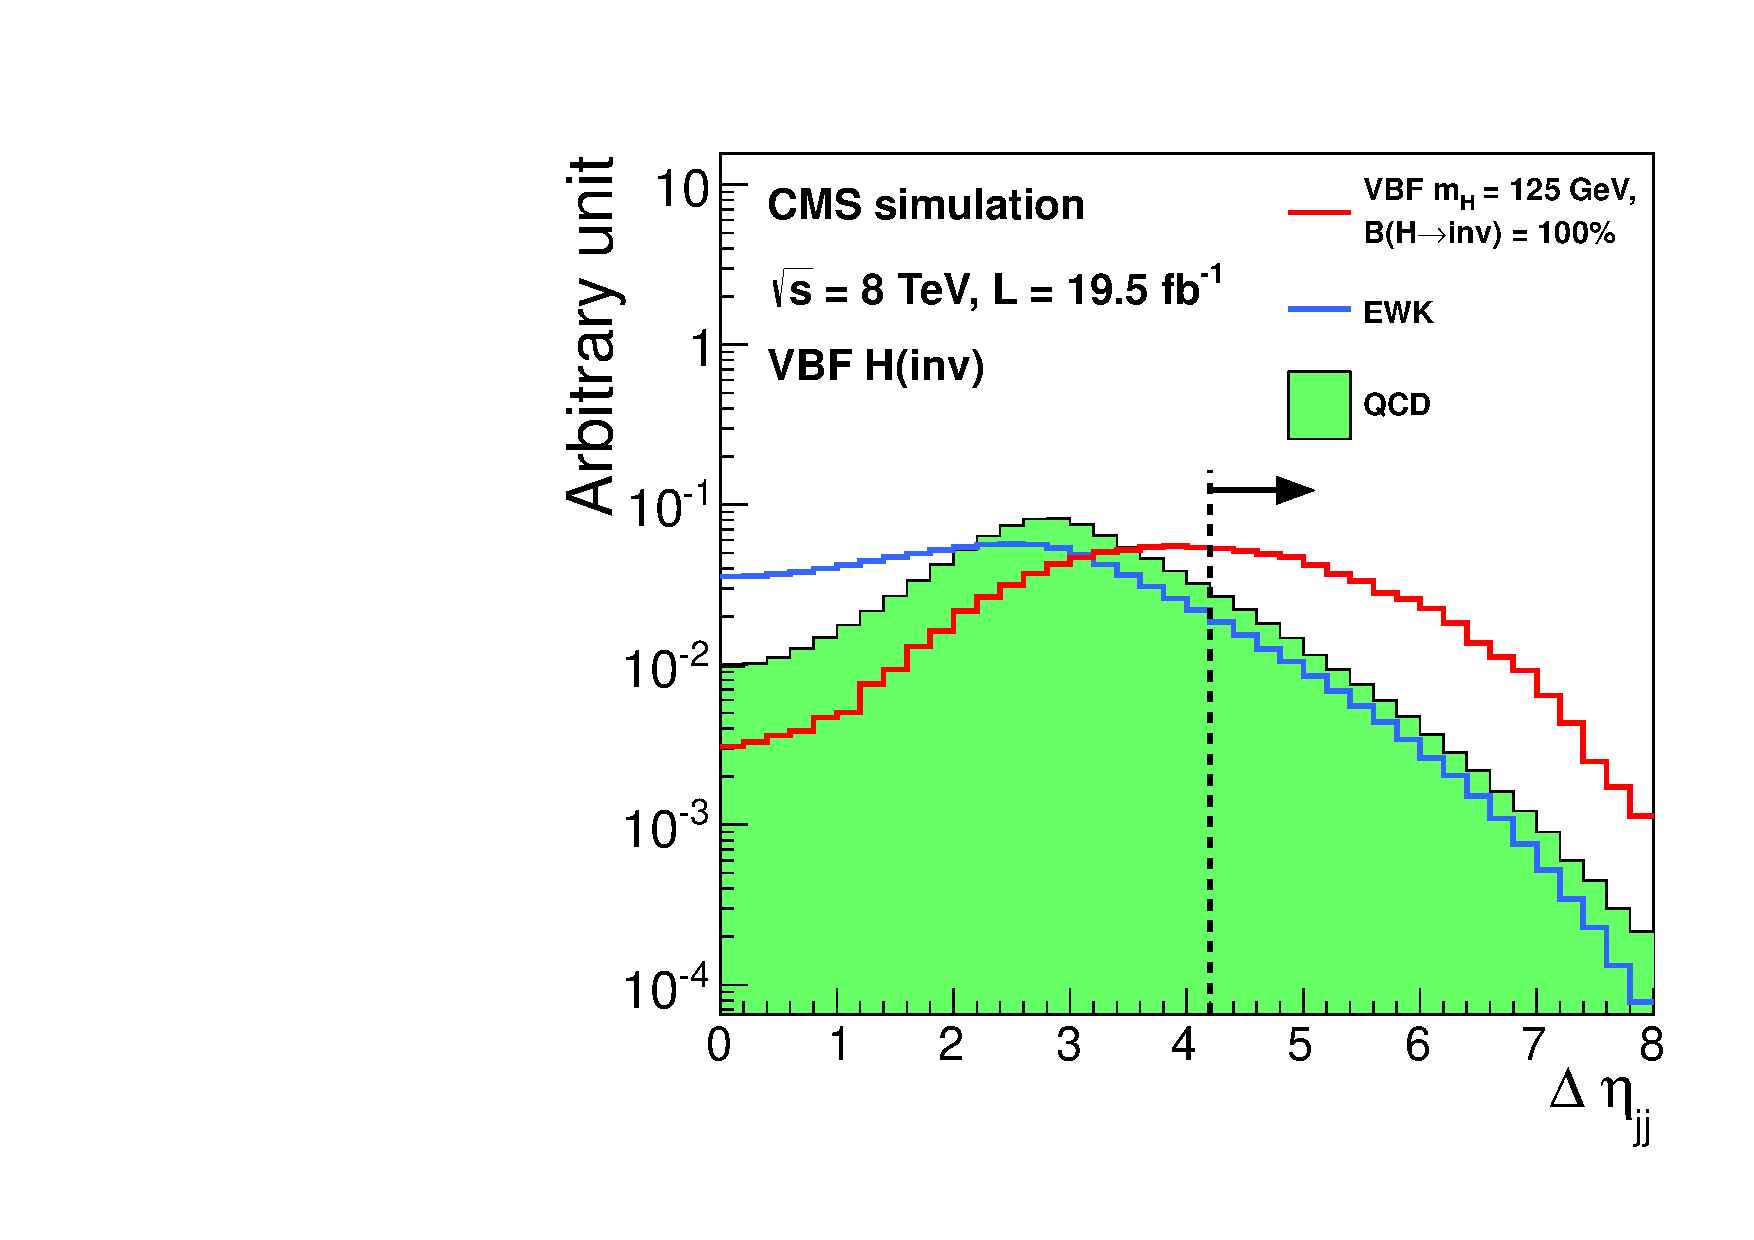
\includegraphics[width=.65\largefigwidth]{plots/prompt/VBF-Dijet-DEta.pdf}}

  \subfloat[]{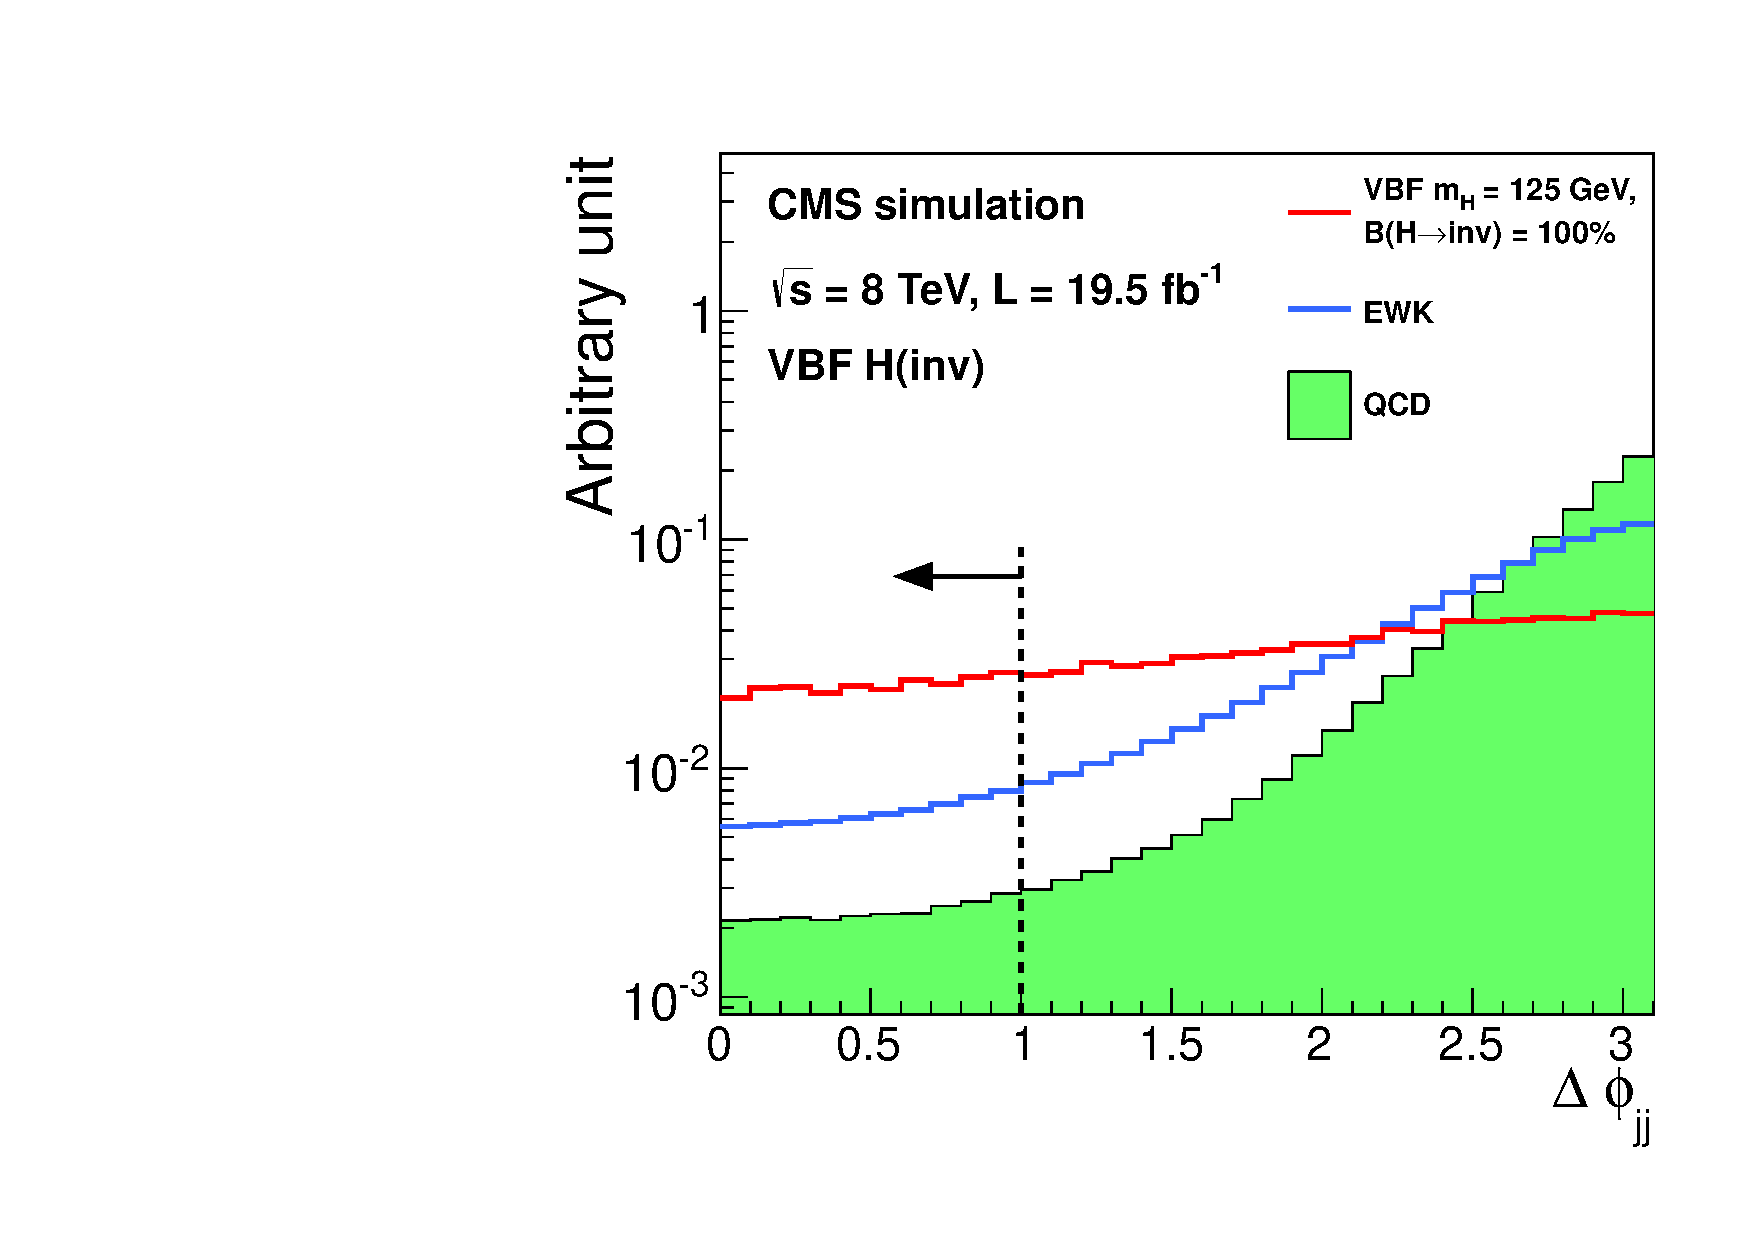
\includegraphics[width=.65\largefigwidth]{plots/prompt/VBF-Dijet-DPhi.pdf}}
  \subfloat[]{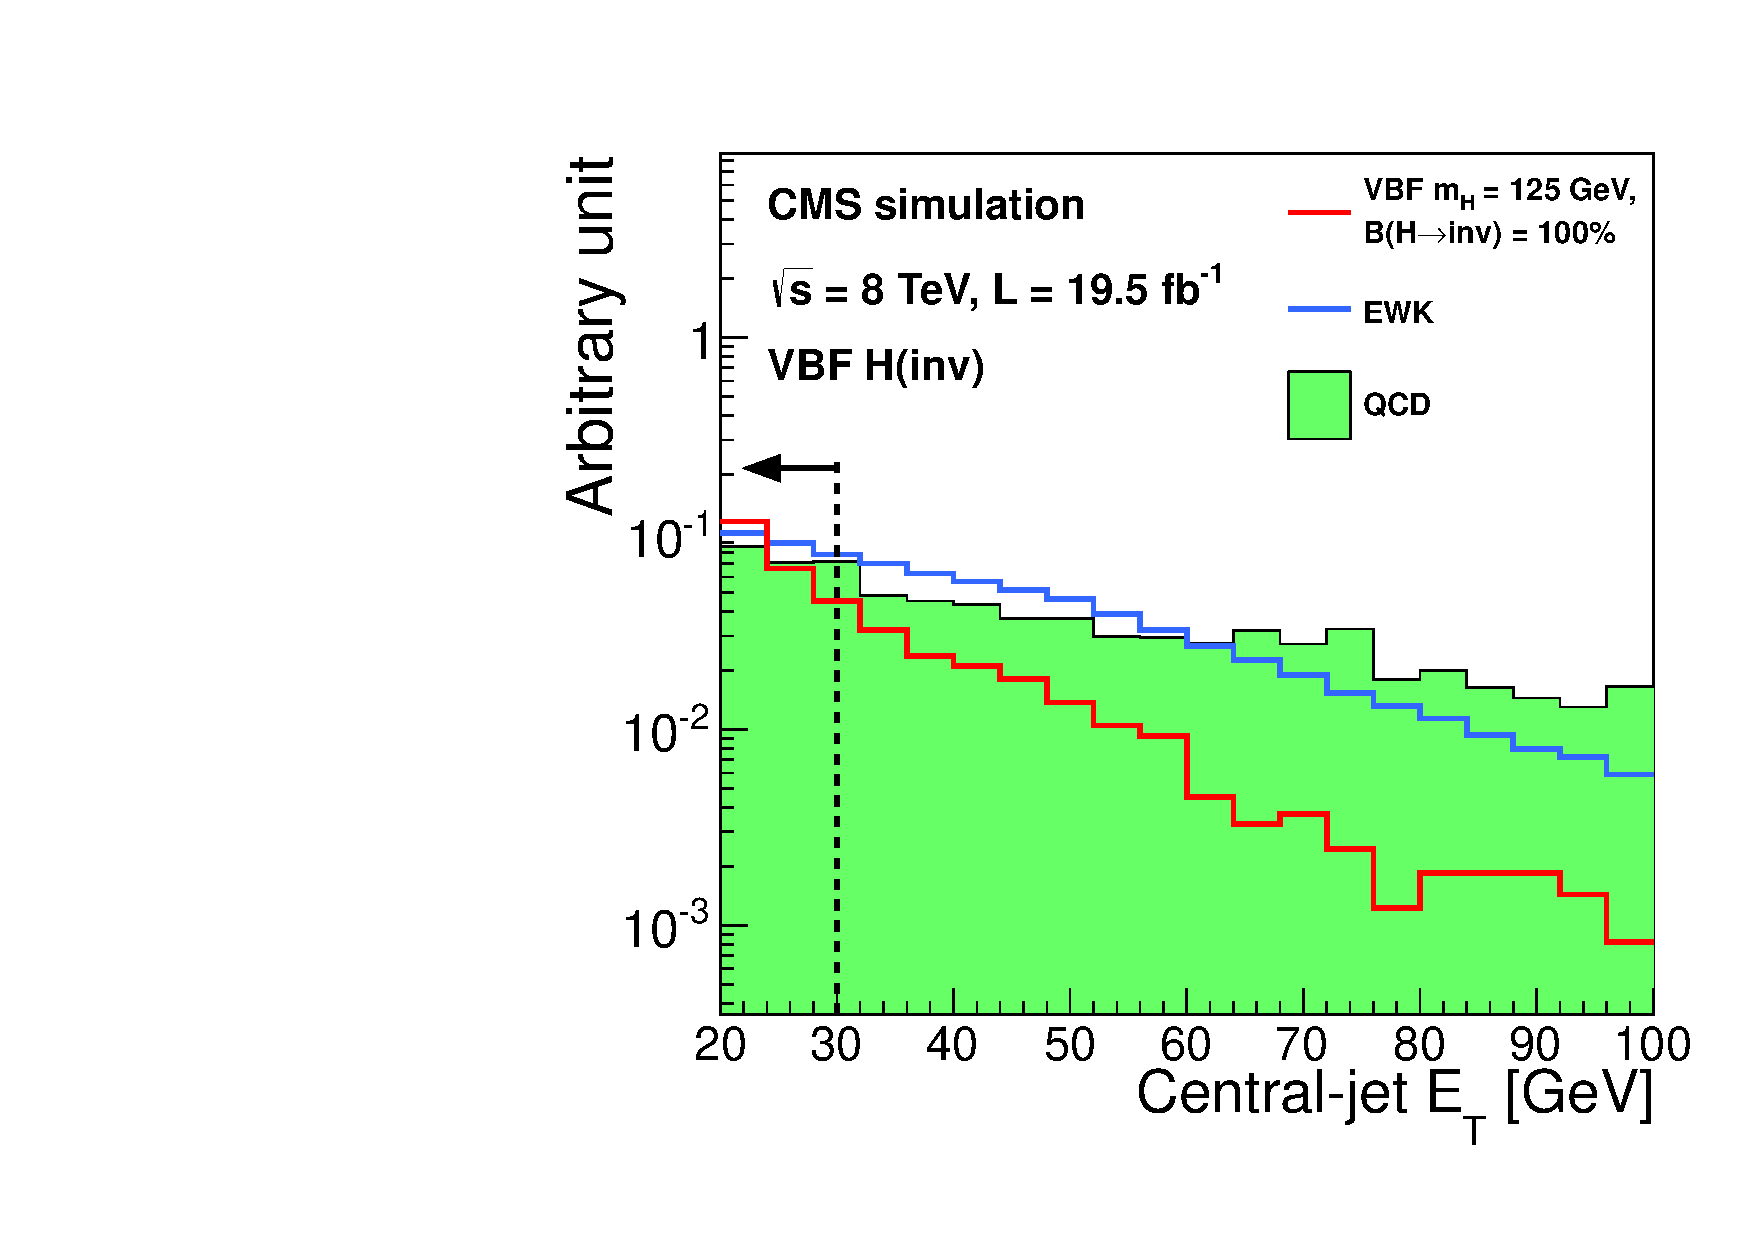
\includegraphics[width=.65\largefigwidth]{plots/prompt/VBF-CJV-pT.pdf}}
  \DIFdelbeginFL %DIFDELCMD < \caption{%%%
\DIFdelendFL \DIFaddbeginFL \caption[Distributions of (a) \Mjj, (b) \detajj, (c) \dphijj and (d) leading central jet \pt in background and signal MC events. The events shown are required to have two jets in opposite forward/backward halves of the detector with \pt$>50$ \GeV, $\Mjj>150$ \GeV and \METnoMU$>130$ \GeV. EWK refers to the V+jets and minor backgrounds described in \SectionRef{sec:promptbkg} and QCD refers to the QCD multijet background. The dashed lines indicate the offline selection criteria applied to these variables, which are motivated in the text.]{\DIFaddendFL Distributions of (a) \Mjj, (b) \detajj, (c) \dphijj and (d) leading central jet \pt in background and signal \DIFdelbeginFL %DIFDELCMD < \ac{MC} %%%
\DIFdelendFL \DIFaddbeginFL \DIFaddFL{MC }\DIFaddendFL events. The events shown are required to have two jets in opposite forward/backward halves of the detector with \pt$>50$ \GeV, $\Mjj>150$ \GeV and \METnoMU$>130$ \GeV. EWK refers to the V+jets and minor backgrounds described in \SectionRef{sec:promptbkg} and \DIFdelbeginFL %DIFDELCMD < \ac{QCD} %%%
\DIFdelendFL \DIFaddbeginFL \DIFaddFL{QCD }\DIFaddendFL refers to the \DIFdelbeginFL %DIFDELCMD < \ac{QCD} %%%
\DIFdelendFL \DIFaddbeginFL \DIFaddFL{QCD }\DIFaddendFL multijet background. The dashed lines indicate the offline selection criteria applied to these variables, which are motivated in the text ~\cite{Chatrchyan:2014tja}.}
  \label{fig:promptcontrolplots}
\end{figure}


\section{Background estimation}
\label{sec:promptbkg}
As discussed in \SectionRef{sec:promptsel} there are several background processes which are capable of producing VBF-like jets in association with \MET. The event selection removes most of these events, however a significant number still remain and it is important to estimate this number precisely. Data-driven methods, \DIFdelbegin \DIFdel{where }\DIFdelend \DIFaddbegin \DIFadd{with }\DIFaddend data ``control regions'' \DIFdelbegin \DIFdel{, }\DIFdelend which are similar to the signal region, are used to estimate the most significant backgrounds. This data-driven approach is particularly important as the very stringent kinematic requirements placed on the tag jets lead to large uncertainties on estimates taken from \ac{MC} alone. The particular method used to estimate each of the backgrounds will be described in this section. \DIFaddbegin \DIFadd{As described in the declaration, I performed a cross-check of the $\PW+$jets background estimation. The tables of the results of and inputs to the $\PW+$jets background estimation in this section are taken from this cross-check. Therefore, whilst the agreement with the published results is good, exact agreement is not expected.
}\DIFaddend 

\subsection{\PW$\rightarrow e\nu$ + jets}
\label{sec:promptwenu}
The $\PW+$jets background where the $\PW$ boson decays to an electron and an electron neutrino, $\PW\rightarrow e\nu$, is estimated using single electron events. All aspects of the event selection are the same as those used in the signal region, except for the electron veto, which is replaced with the requirement that there is exactly one tight electron in the event and no other veto electrons. These requirements give a single electron control region composed of events with jets that have the same kinematics as those in the signal region, but which is dominated by $\PW\rightarrow e\nu$ events.

The number of $\PW\rightarrow e\nu$ events in the signal region is then estimated by using the ratio between the expected number of events in the signal and control regions from \ac{MC} to extrapolate from the number of events seen in data in the single electron control region using the following formula:
\begin{equation}
  \label{eq:wdatabkg}
  N^{S}_{Exp}=\left(N^{C}_{Data}-N^{C}_{Bkg}\right)\cdot\frac{N^{S}_{MC}}{N^{C}_{MC}},
\end{equation}
where $N^{S}_{Exp}$ is the number of expected events in the signal region from this background process, $N^{C}_{Data}$ is the number of events seen in the control region in data, $N^{C}_{Bkg}$ is the number of events from other backgrounds in the control region estimated using \ac{MC}, which is expected to be small, and $N^{S}_{MC}$ and $N^{C}_{MC}$ are the numbers of events predicted by \ac{MC} to be in the signal and control regions respectively. The fact that estimations from \ac{MC} are only used in ratios, or where they are expected to be small, significantly reduces the dependence of the final background estimation on the overall rate of the process predicted by \ac{MC} and instead allows the observed rate in data to be used. It is important that the shape of the variables which differ between the control and signal regions are well modelled by the \ac{MC}. The modelling of the shape of two key variables, the \METnoMU and the electron \pt, are shown in \FigureRef{fig:promptwenu}. It can be seen that whilst the overall rate is significantly different between data and \ac{MC}, the shape of the distribution is modelled well. \DIFaddbegin \DIFadd{Furthermore, as a closure test $N^{S}_{MC}$ was replaced with the number of }\ac{MC} \DIFadd{events expected in the control regions used for other background processes and good agreement was seen. }\DIFaddend The inputs to, and results of, the background estimation are shown in \TableRef{tab:promptwenu}.

%tables from AN-13-205
\begin{table}
  \caption{The inputs to, and results of, the \DIFaddbeginFL \DIFaddFL{cross-check performed by the author of the }\DIFaddendFL $\PW\rightarrow e\nu$ background estimation. $N_{\PW\rightarrow e\nu}$ is, for the signal region the number of events expected from $\PW\rightarrow e\nu$ backgrounds, and for the control region the number of events remaining in the region after the subtraction of other backgrounds.}
  \label{tab:promptwenu}
  \begin{tabular}{lcc}
    \hline
    \hline
    & Signal region & Control region \\
    \hline
    \hline
    $N_{Data}$ & N/A & 64\\
    $N_{Bkg}$ & N/A & $7.42\pm2.78$(\ac{MC} stat.) \\
    $N_{MC}$& $105\pm10$(\ac{MC} stat.) & $86.6\pm 7.1$(\ac{MC} stat.) \\
    \hline
    \DIFaddbeginFL \DIFaddFL{$\frac{N^{data}-N^{bkg}}{N^{C}_{MC}}$ }& \multicolumn{2}{c|}{0.65$\pm$0.09\stat$\pm$0.06(MC stat)} \\
    \hline
    \DIFaddendFL $N_{\PW\rightarrow e\nu}$& \textcolor{red}{$68.7\pm 10.3\stat\pm 8.8$(MC stat.)} & $56.6\pm 8.5\stat$ \\
    \hline
    \hline
  \end{tabular}
\end{table}

%plot from AN-12-403
\begin{figure}
  \subfloat[]{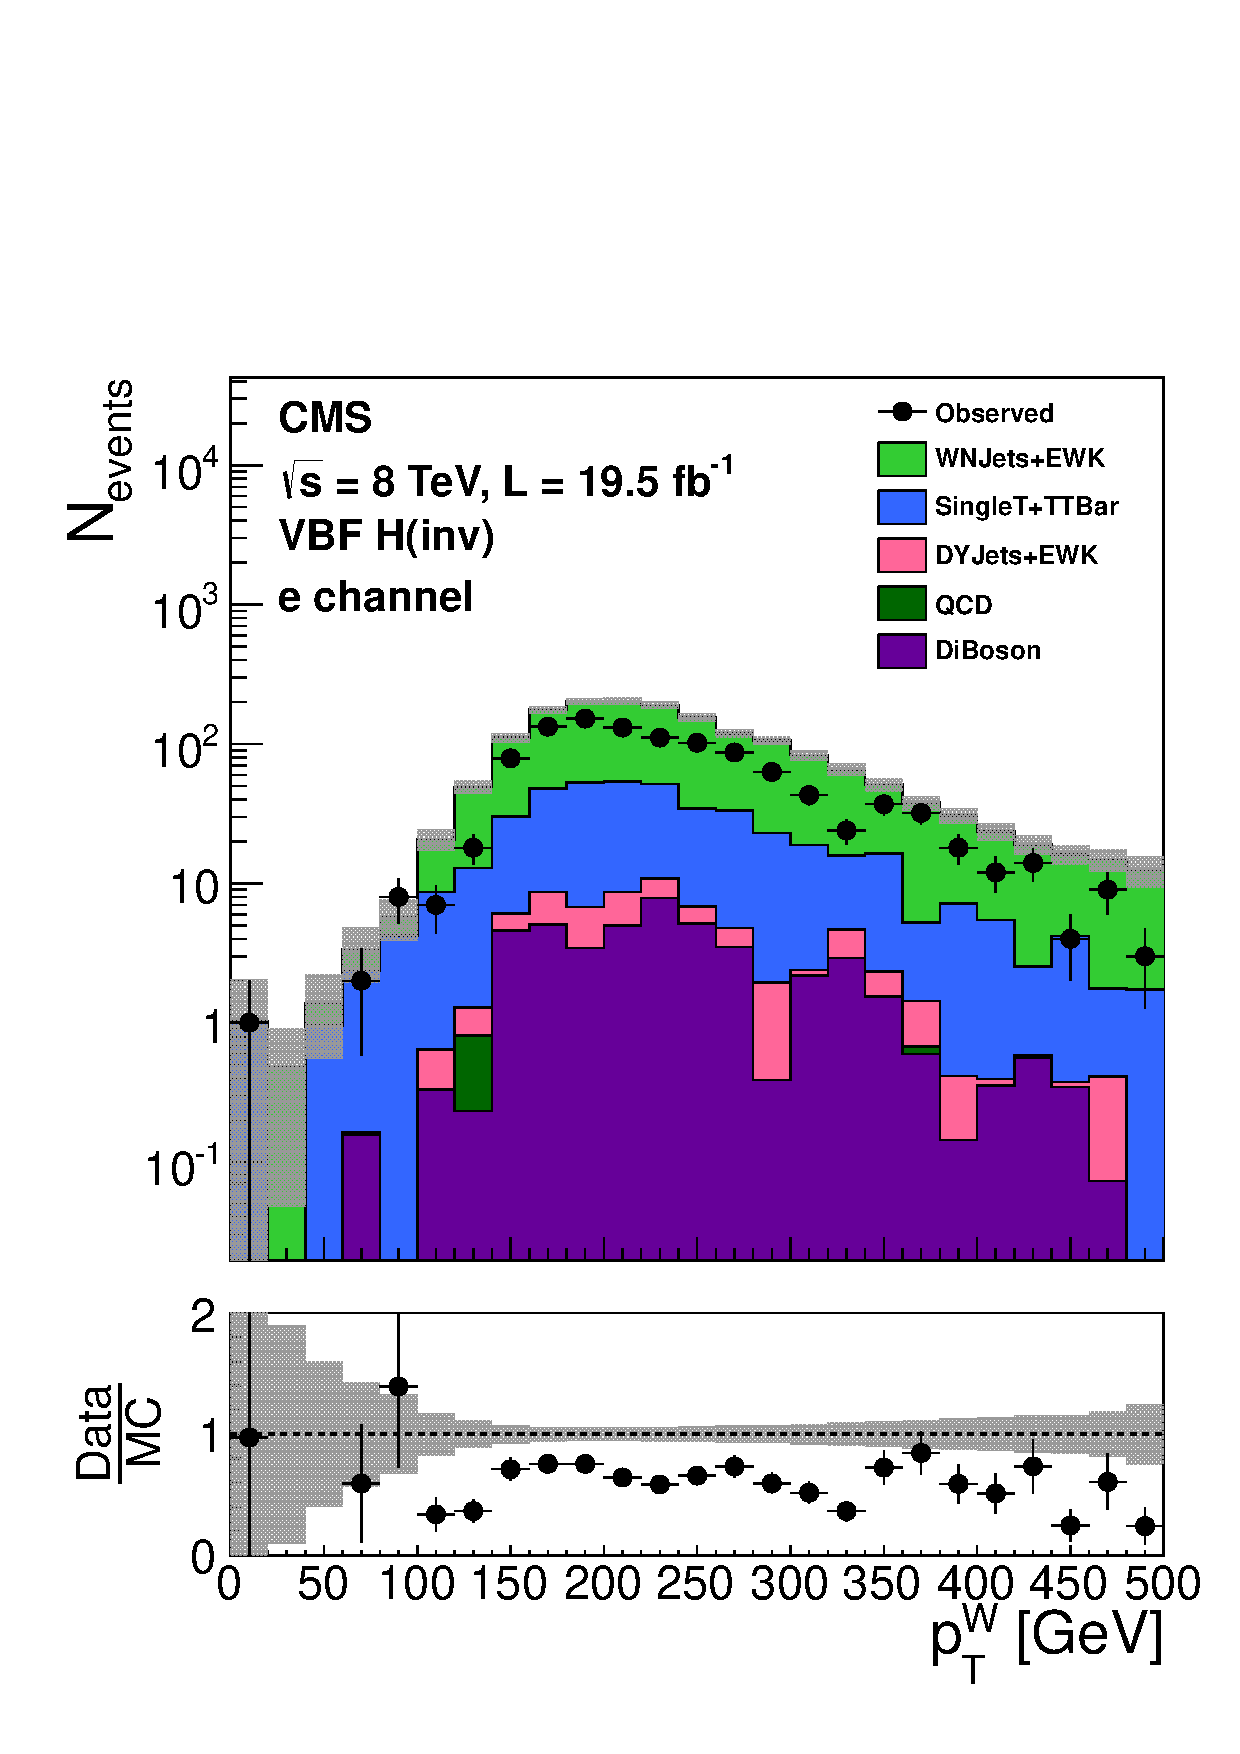
\includegraphics[width=.65\largefigwidth]{plots/prompt/AN-12-403-figs/hWEl_WpT.pdf}}
  \subfloat[]{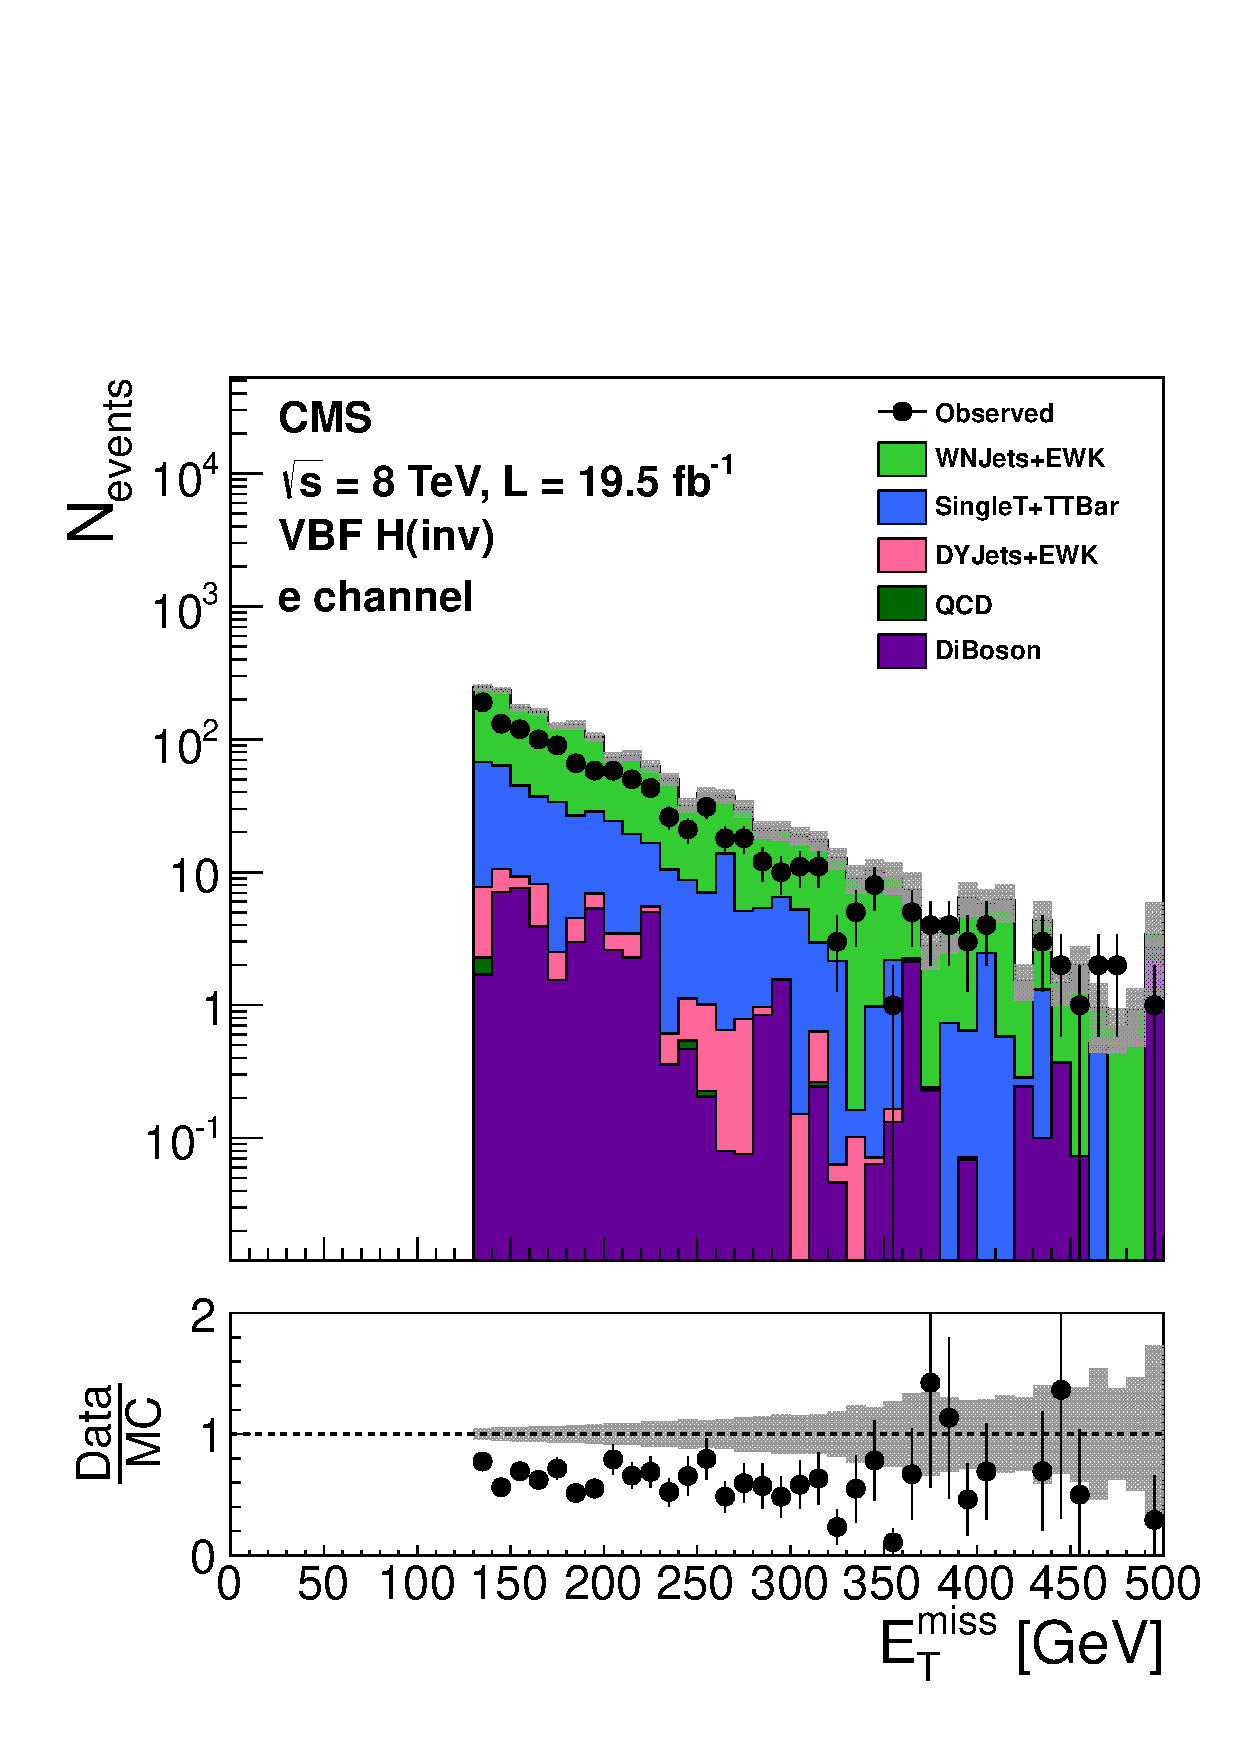
\includegraphics[width=.65\largefigwidth]{plots/prompt/AN-12-403-figs/hWEl_MET.pdf}}
  \DIFdelbeginFL %DIFDELCMD < \caption{%%%
\DIFdelendFL \DIFaddbeginFL \caption[Distributions of the visible $\PW$ boson \pt (i.e. the electron \pt) (a) and \METnoMU (b) in the single electron control region. WNJets+EWK indicates the W+jets contribution to this region, SingleT+TTBar indicates the contribution from top quark related processes, DYJets+EWK indicates the Z+jets contribution, QCD indicates the QCD multijet contribution and DiBoson indicates the two vector boson contribution. All of these contributions are estimated from MC. The hatched region illustrates the systematic uncertainty. Whilst the overall rate of data and MC is very different, the shape can be seen to agree well.]{\DIFaddendFL Distributions of the visible $\PW$ boson \pt (i.e. the electron \pt) (a) and \METnoMU (b) in the single electron control region. WNJets+EWK indicates the W+jets contribution to this region, SingleT+TTBar indicates the contribution from top quark related processes, DYJets+EWK indicates the Z+jets contribution, \DIFdelbeginFL %DIFDELCMD < \ac{QCD} %%%
\DIFdelendFL \DIFaddbeginFL \DIFaddFL{QCD }\DIFaddendFL indicates the \DIFdelbeginFL %DIFDELCMD < \ac{QCD} %%%
\DIFdelendFL \DIFaddbeginFL \DIFaddFL{QCD }\DIFaddendFL multijet contribution and DiBoson indicates the two vector boson contribution. All of these contributions are estimated from \DIFdelbeginFL %DIFDELCMD < \ac{MC}%%%
\DIFdelendFL \DIFaddbeginFL \DIFaddFL{MC}\DIFaddendFL . The hatched region illustrates the systematic uncertainty~\cite{ARTICLE:CMSAN-12-403}. Whilst the overall rate of data and \DIFdelbeginFL %DIFDELCMD < \ac{MC} %%%
\DIFdelendFL \DIFaddbeginFL \DIFaddFL{MC }\DIFaddendFL is very different, the shape can be seen to agree well.}
  \label{fig:promptwenu}
\end{figure}

\subsection{\PW$\rightarrow \mu\nu$ + jets}
\label{sec:promptwmunu}
The method used to estimate the background from $\PW$+jets where the $\PW$ boson decays to a muon and a muon neutrino, $\PW\rightarrow\mu\nu$, is very similar to that used for $\PW\rightarrow e\nu$. A single muon control region is used which replaces the muon veto of the signal region with a requirement that there is exactly one tight muon and no other veto muons. All other signal region cuts remain unchanged. Equation \ref{eq:wdatabkg} is then used, with the control region now being the single muon control region, to estimate the number of events from $W\rightarrow\mu\nu$ expected in the signal region. The inputs to, and results of, the background estimation are shown in \TableRef{tab:promptwmunu}, and distributions of the muon \pt and the \METnoMU in the single muon control region are shown in \FigureRef{fig:promptwmunu}.

%tables from AN-13-205
\begin{table}
  \caption{The inputs to, and results of, the $\PW\rightarrow \mu\nu$ background estimation. $N_{\PW\rightarrow \mu\nu}$ is, for the signal region the number of events expected from $\PW\rightarrow \mu\nu$ backgrounds, and for the control region the number of events remaining in the region after the subtraction of other backgrounds.}
  \label{tab:promptwmunu}
  \begin{tabular}{lcc}
    \hline
    \hline
    & Signal region & Control region \\
    \hline
    \hline
    $N_{Data}$ & N/A & 216\\
    $N_{Bkg}$ & N/A & $30.1\pm 4.5$(\ac{MC} stat.) \\
    $N_{MC}$& $108\pm 10$(\ac{MC} stat.) & $306\pm 15$(\ac{MC} stat.) \\
    \hline
    \DIFaddbeginFL \DIFaddFL{$\frac{N^{data}-N^{bkg}}{N^{C}_{MC}}$ }& \multicolumn{2}{c|}{$0.61\pm$0.05\stat$\pm$0.03(MC stat)} \\
    \hline
    \DIFaddendFL $N_{\PW\rightarrow \mu\nu}$& \textcolor{red}{$65.8\pm 5.4\stat\pm 6.7$(MC stat.)} & $186\pm 15\stat$ \\
    \hline
    \hline
  \end{tabular}
\end{table}

%plot from AN-12-403
\begin{figure}
  \subfloat[]{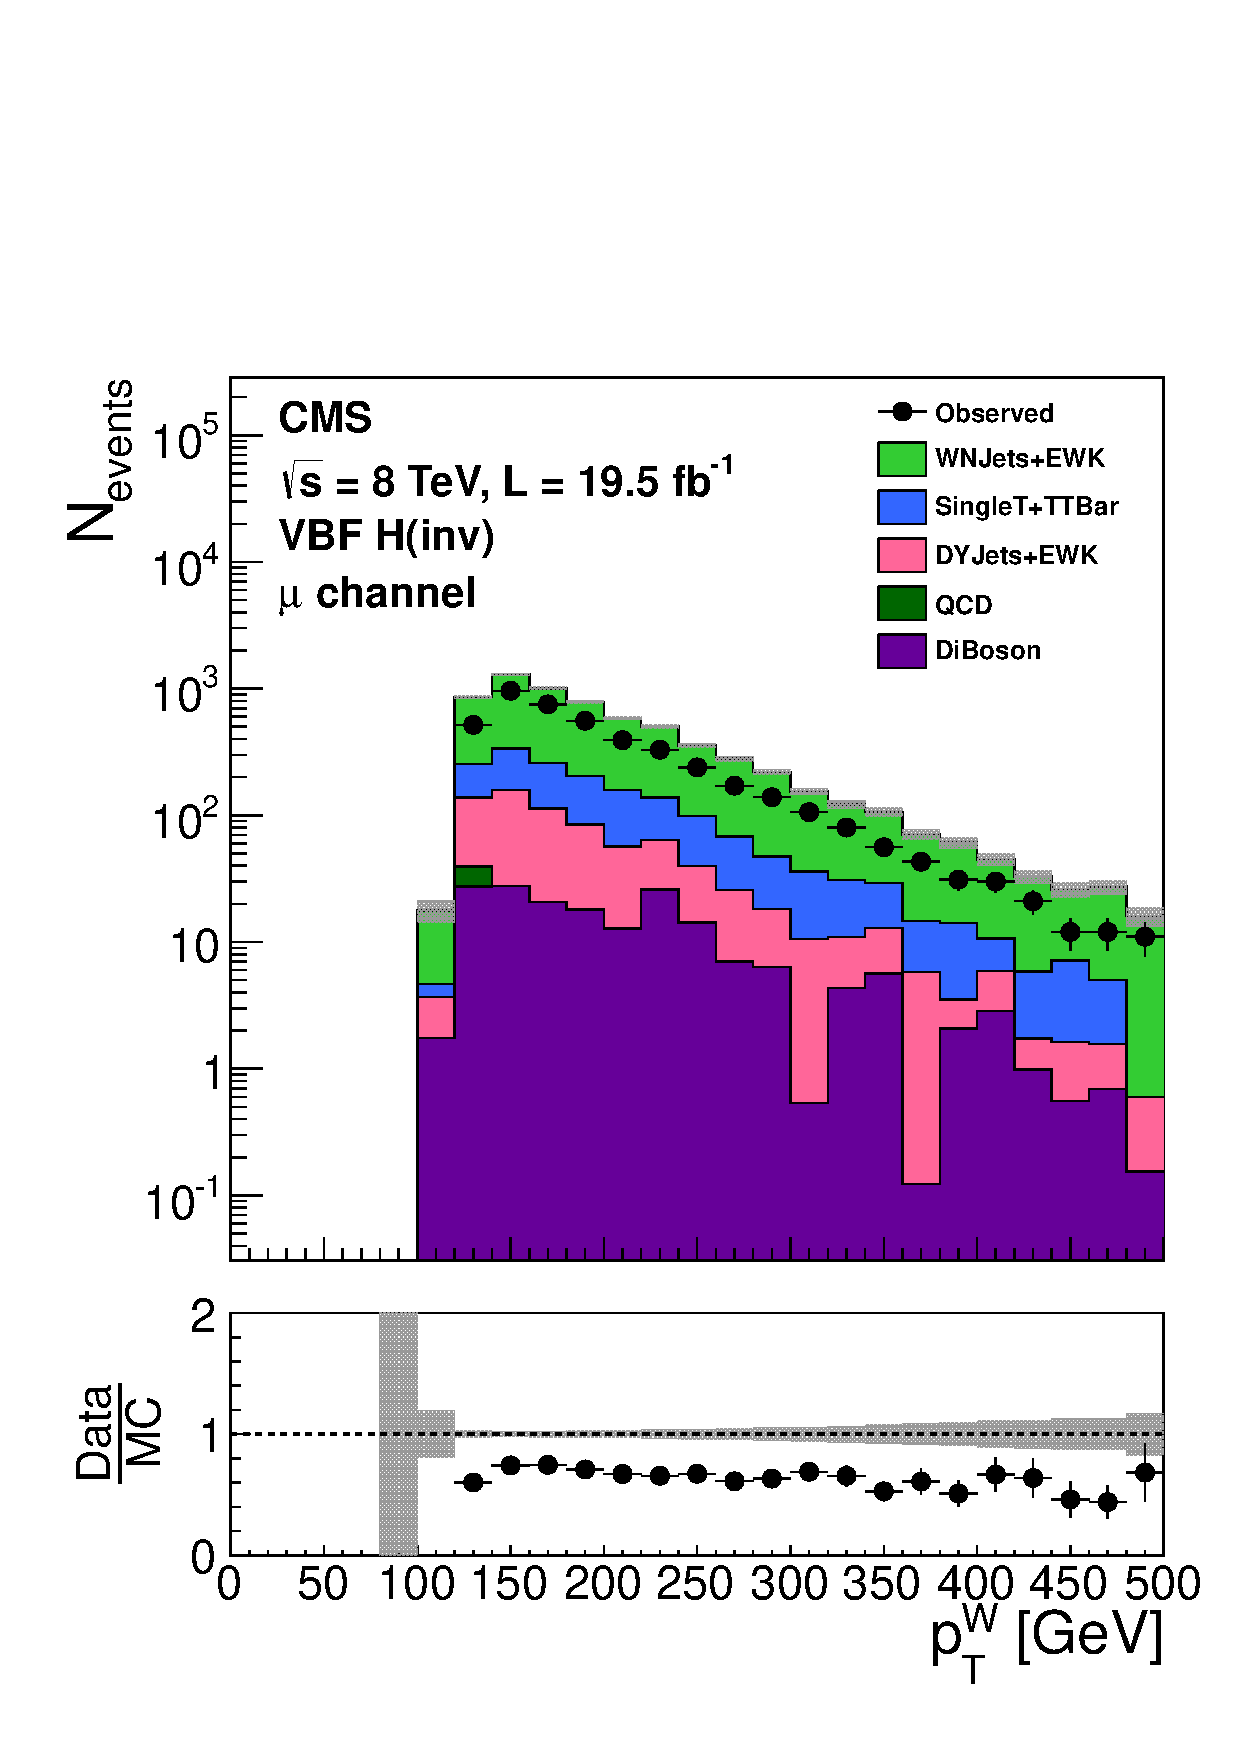
\includegraphics[width=.65\largefigwidth]{plots/prompt/AN-12-403-figs/hWMu_WpT.pdf}}
  \subfloat[]{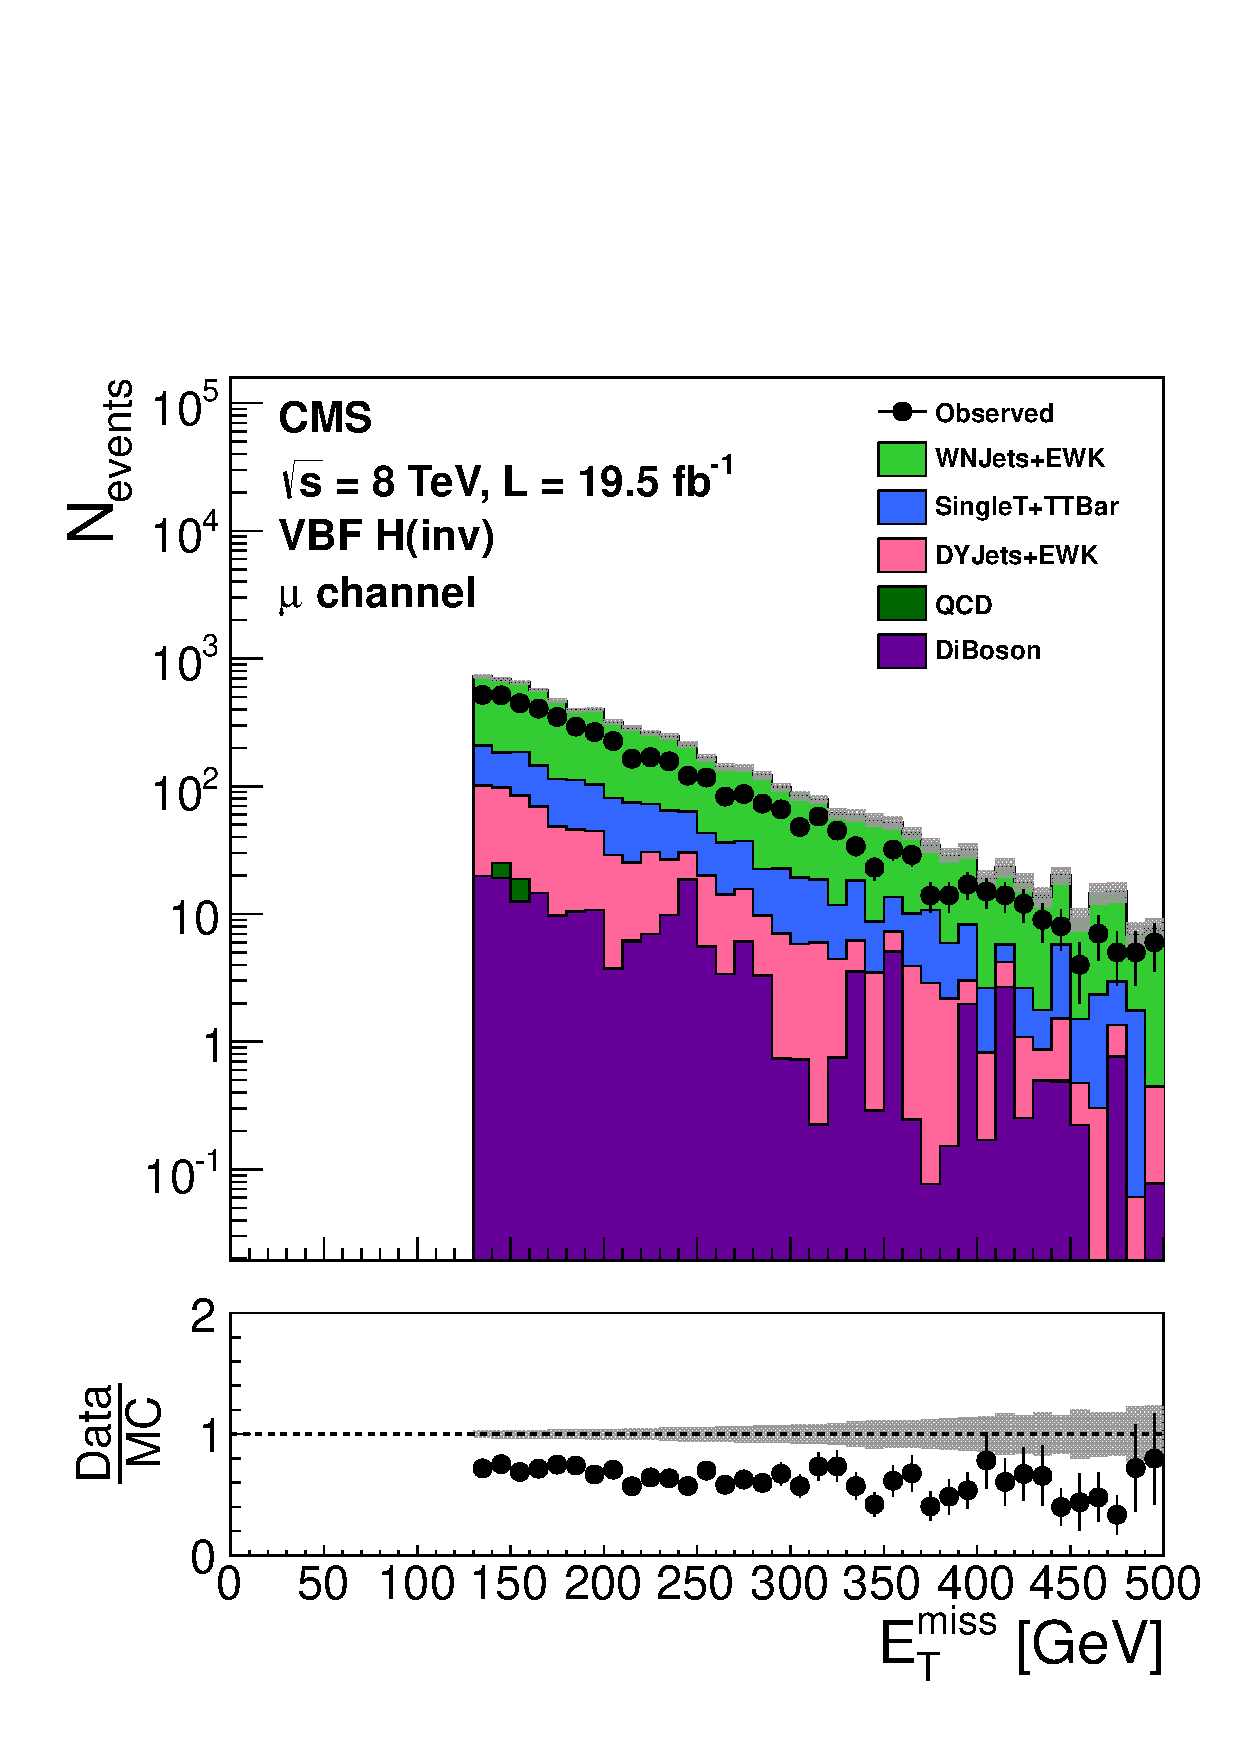
\includegraphics[width=.65\largefigwidth]{plots/prompt/AN-12-403-figs/hWMu_MET.pdf}}
  \DIFdelbeginFL %DIFDELCMD < \caption{%%%
\DIFdelendFL \DIFaddbeginFL \caption[Distributions of the visible $\PW$ boson \pt (i.e. the muon \pt) (a) and \METnoMU (b) in the single muon control region. WNJets+EWK indicates the W+jets contribution to this region, SingleT+TTBar indicates the contribution from top quark related processes, DYJets+EWK indicates the Z+jets contribution, QCD indicates the QCD multijet contribution and DiBoson indicates the two vector boson contribution. All of these contributions are estimated from MC. The hatched region illustrates the systematic uncertainty. Whilst the overall rate of data and MC is very different, the shape can be seen to agree well.]{\DIFaddendFL Distributions of the visible $\PW$ boson \pt (i.e. the muon \pt) (a) and \METnoMU (b) in the single muon control region. WNJets+EWK indicates the W+jets contribution to this region, SingleT+TTBar indicates the contribution from top quark related processes, DYJets+EWK indicates the Z+jets contribution, \DIFdelbeginFL %DIFDELCMD < \ac{QCD} %%%
\DIFdelendFL \DIFaddbeginFL \DIFaddFL{QCD }\DIFaddendFL indicates the \DIFdelbeginFL %DIFDELCMD < \ac{QCD} %%%
\DIFdelendFL \DIFaddbeginFL \DIFaddFL{QCD }\DIFaddendFL multijet contribution and DiBoson indicates the two vector boson contribution. All of these contributions are estimated from \DIFdelbeginFL %DIFDELCMD < \ac{MC}%%%
\DIFdelendFL \DIFaddbeginFL \DIFaddFL{MC}\DIFaddendFL . The hatched region illustrates the systematic uncertainty~\cite{ARTICLE:CMSAN-12-403}. Whilst the overall rate of data and \DIFdelbeginFL %DIFDELCMD < \ac{MC} %%%
\DIFdelendFL \DIFaddbeginFL \DIFaddFL{MC }\DIFaddendFL is very different, the shape can be seen to agree well.}
  \label{fig:promptwmunu}
\end{figure}

\subsection{\PW$\rightarrow \tau\nu$ + jets}
\label{sec:promptwtaunu}
The background from $\PW$+jets where the $\PW$ boson decays to a tau and a tau neutrino, $\PW\rightarrow\tau\nu$, is estimated using a single tau control region data-driven method. However, in this case the control region used has more differences from the signal region than those used above. The reason for these increased differences is that the reconstruction efficiency for tau leptons is significantly lower than that for electrons or muons, and they are also more likely to be misreconstructed as jets, causing the event to be vetoed by the \ac{CJV}. There are therefore only $3.76\pm 1.27\stat$ $\PW\rightarrow\tau\nu$ events with identified taus with \pt$>20$ \GeV expected in the signal region from \ac{MC}.

To increase the number of events in the single tau control region, the \ac{CJV} has been removed. The resulting control region has $29.2\pm 3.61\stat$ $\PW+$jets events expected and thus a much lower statistical uncertainty. As there is no veto of tau leptons in the signal region the tau control region and the signal region are not mutually exclusive. However, as stated above the number of events in the signal region with identified taus is expected to be small, so the overlap is considered negligible.

%cross-check of tau discriminant https://indico.cern.ch/event/259915/session/1/contribution/2/attachments/458506/635408/tauid090713.pdf
In addition to the tau identification algorithm described in \SectionRef{sec:taus}, alternative algorithms were studied to check for better performance in terms of identification efficiency and fake rate. Specifically\DIFaddbegin \DIFadd{, }\DIFaddend an alternative isolation algorithm was investigated which used a \ac{MVA} approach to estimate the isolation sum, as well as different working points for the anti-electron and anti-muon discriminators~\cite{CMS-PAS-TAU-11-001}. The tau identification efficiency was found to be higher for both the alternative isolation algorithm and different working points for the anti-lepton discriminators, being twice as large if both were used compared to the standard tau identification. However, the rate of $\PW\rightarrow e\nu$ events being identified as $\PW\rightarrow\tau\nu$ was also significantly increased, going from 2\% for the standard identification to 15\% when the alternative isolation and anti-lepton discriminators were used. It was therefore decided to use the tau identification described in \SectionRef{sec:taus}.

The final estimation of the background from $W\rightarrow\tau\nu$ is carried out using \EquationRef{eq:wdatabkg}, with the single tau control region with no \ac{CJV} being used as the control region. The inputs to, and results of, the background estimation are shown in \TableRef{tab:promptwtaunu}. Distributions of the tau \pt and \dphijj in the single tau control region are shown in \FigureRef{fig:promptwtaunu}\DIFdelbegin \DIFdel{, }\DIFdelend \DIFaddbegin \DIFadd{; }\DIFaddend it can be seen that the shape of the two distributions in data and \ac{MC} agree well with the exception of the high \dphijj region which is not part of either the signal or tau control regions.

%tables from AN-13-205
\begin{table}
  \caption{The inputs to, and results of, the $\PW\rightarrow \tau\nu$ background estimation. $N_{\PW\rightarrow \tau\nu}$ is, for the signal region the number of events expected from $\PW\rightarrow \tau\nu$ backgrounds, and in the control region the number of events remaining in the region after the subtraction of other backgrounds.}
  \label{tab:promptwtaunu}
  \begin{tabular}{lcc}
    \hline
    \hline
    & Signal region & Control region \\
    \hline
    \hline
    $N_{Data}$ & N/A & 32\\
    $N_{Bkg}$ & N/A & $14.7\pm 3.4$(\ac{MC} stat.) \\
    $N_{MC}$& $95.6\pm 8.5$(\ac{MC} stat.) & $29.2\pm 3.6$(\ac{MC} stat.) \\
    \hline
    \DIFaddbeginFL \DIFaddFL{$\frac{N^{data}-N^{bkg}}{N^{C}_{MC}}$ }& \multicolumn{2}{c|}{$0.59\pm$0.19\stat$\pm$0.10(MC stat)} \\
    \hline
    \DIFaddendFL $N_{\PW\rightarrow \tau\nu}$& \textcolor{red}{$56.5\pm 21.5\stat\pm 8.6$(MC stat.)} & $17.3\pm 3.9 \stat$ \\
    \hline
    \hline
  \end{tabular}
\end{table}

%plot from AN-12-403
\begin{figure}
  \subfloat[]{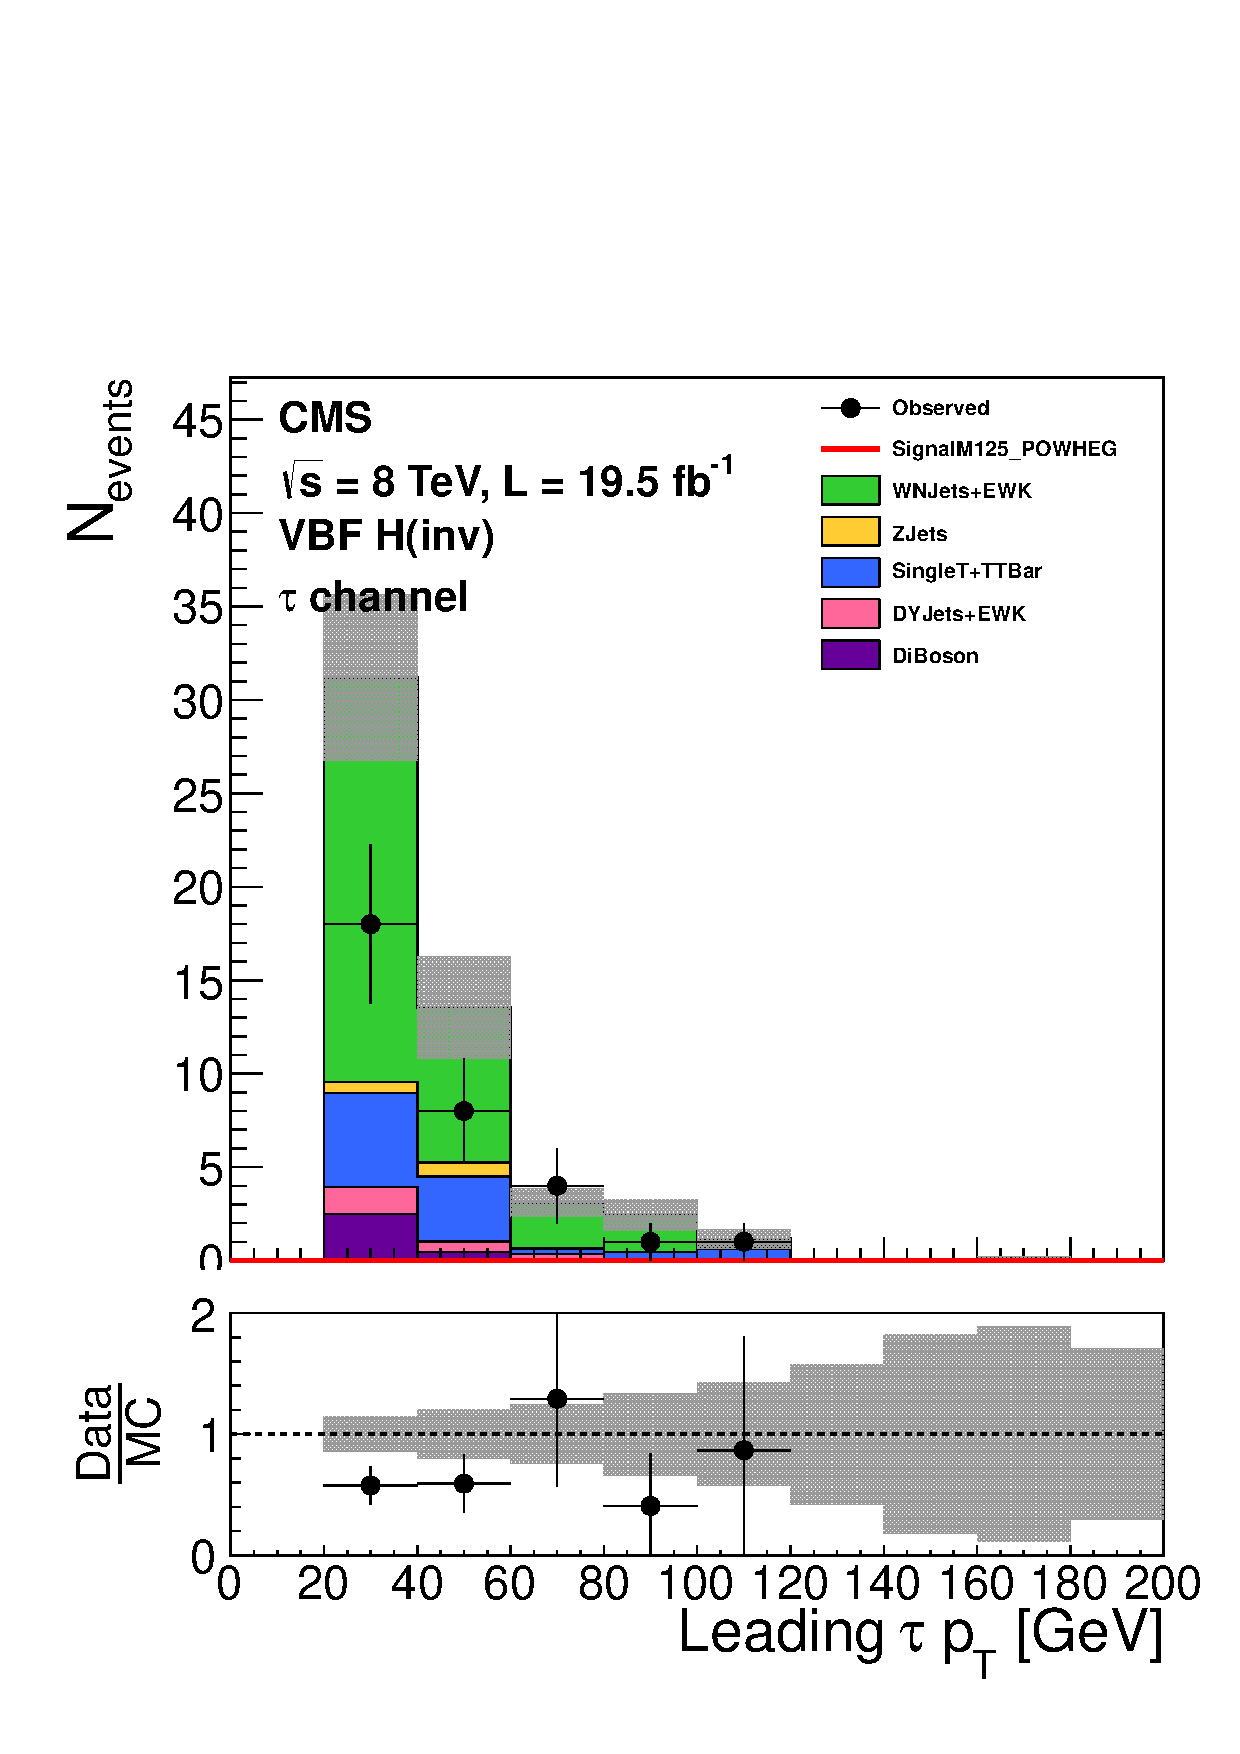
\includegraphics[width=.65\largefigwidth]{plots/prompt/AN-12-403-figs/hWTau_tau1Pt.pdf}}
  \subfloat[]{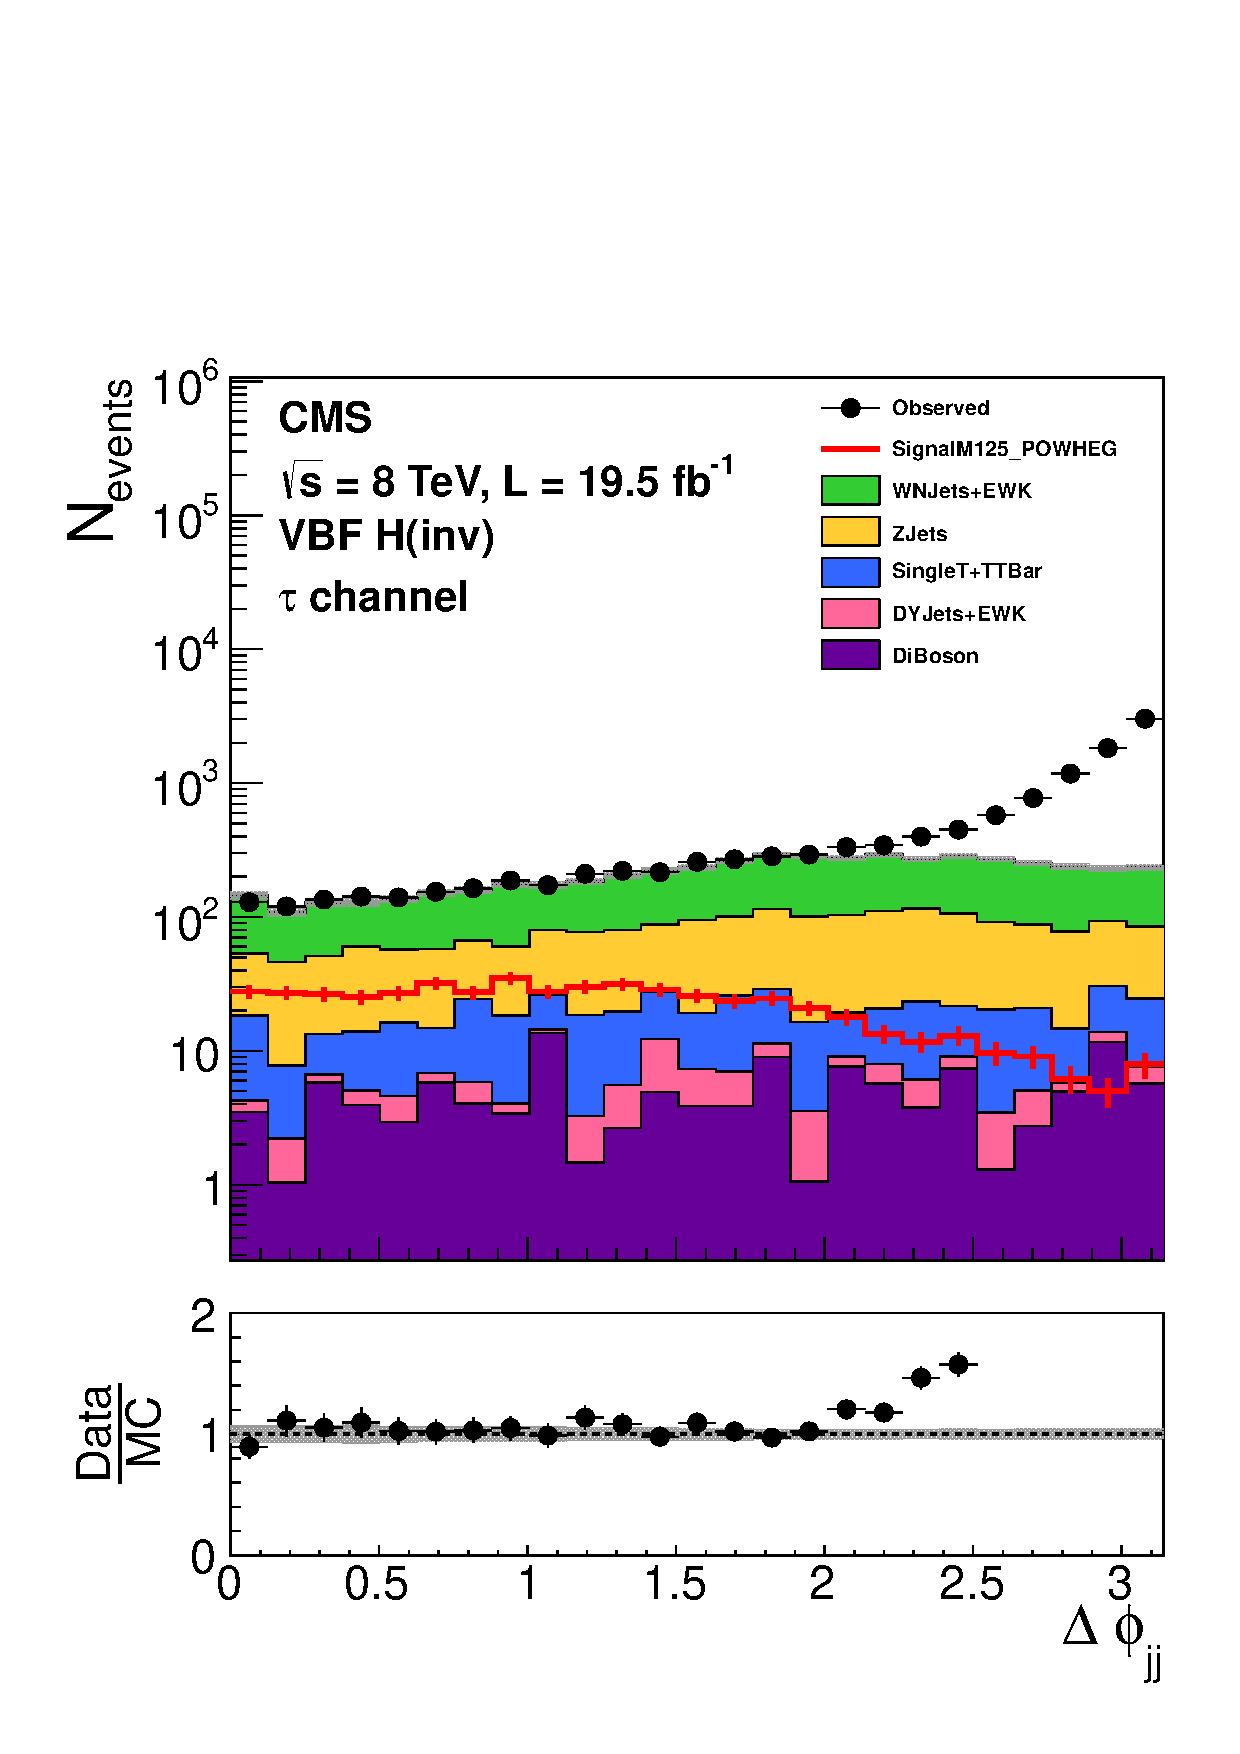
\includegraphics[width=.65\largefigwidth]{plots/prompt/AN-12-403-figs/hWTau_dPhiJJ.pdf}}
  \DIFdelbeginFL %DIFDELCMD < \caption{%%%
\DIFdelendFL \DIFaddbeginFL \caption[Distributions of the the tau \pt (a) and \dphijj (b) in the single tau control region. WNJets+EWK indicates the W+jets contribution to this region, ZJets indicates the contribution from Z+jets, SingleT+TTBar indicates the contribution from top quark related processes, QCD indicates the QCD multijet contribution and DiBoson indicates the two vector boson contribution. All of these contributions are estimated from MC. The hatched region illustrates the systematic uncertainty.]{\DIFaddendFL Distributions of the the tau \pt (a) and \dphijj (b) in the single tau control region. WNJets+EWK indicates the W+jets contribution to this region, ZJets indicates the contribution from Z+jets, SingleT+TTBar indicates the contribution from top quark related processes, \DIFdelbeginFL %DIFDELCMD < \ac{QCD} %%%
\DIFdelendFL \DIFaddbeginFL \DIFaddFL{QCD }\DIFaddendFL indicates the \DIFdelbeginFL %DIFDELCMD < \ac{QCD} %%%
\DIFdelendFL \DIFaddbeginFL \DIFaddFL{QCD }\DIFaddendFL multijet contribution and DiBoson indicates the two vector boson contribution. All of these contributions are estimated from \DIFdelbeginFL %DIFDELCMD < \ac{MC}%%%
\DIFdelendFL \DIFaddbeginFL \DIFaddFL{MC}\DIFaddendFL . The hatched region illustrates the systematic uncertainty~\cite{ARTICLE:CMSAN-12-403}.}
  \label{fig:promptwtaunu}
\end{figure}

\subsection{\PZ$\rightarrow \nu\nu$ + jets}
\label{sec:promptznunu}
The background from $\PZ+$jets where the \PZ decays to neutrinos, \Znunu, is different from the $\PW+$jets backgrounds described above, in that nothing is required to be misidentified in order for these events to contribute to the signal region. The method used to estimate the \Znunu background therefore differs slightly from that used above. The method uses a dimuon control region which is populated by events from the process \Zmumu. As this process can be mediated by a photon, the kinematics of the jets in \Zmumu events can be different to those from \Znunu. The dimuon control region that is defined therefore has a requirement that the invariant mass of the dimuons be between 60 and 120 \GeV. The control region is otherwise identical to the signal region, except that the muon veto is replaced with a requirement that there are exactly two tight muons and no other veto muons.

As well as the possibility of different kinematics, \Zmumu and \DIFdelbegin \DIFdel{$\PZ/\rightarrow\nu\nu$ }\DIFdelend \DIFaddbegin \DIFadd{$\PZ\rightarrow\nu\nu$ }\DIFaddend also have different cross-sections. The formula used to estimate the \DIFdelbegin \DIFdel{$\PZ/\rightarrow\nu\nu$ }\DIFdelend \DIFaddbegin \DIFadd{$\PZ\rightarrow\nu\nu$ }\DIFaddend background takes this into account as follows:
\begin{equation}
  \label{eq:zdatabkg}
  N^{S}_{Exp}=\left(N^{C}_{Data}-N^{C}_{Bkg}\right)\cdot\frac{\sigma\left(\PZ\rightarrow\nu\nu\right)}{\sigma\left(\PZ/\gamma^{*}\rightarrow\mu\mu\right)}\cdot\DIFdelbegin \DIFdel{\frac{\epsilon^{S}_{VBF}}{\epsilon^{C}_{VBF}}}\DIFdelend \DIFaddbegin \DIFadd{\frac{\epsilon^{S}_{\mbox{VBF}}}{\epsilon^{C}_{\mbox{VBF}}}}\DIFaddend ,
\end{equation}
where $\sigma\left(\PZ\rightarrow\nu\nu\right)$ is the cross-section for \Znunu and $\sigma\left(\PZ/\gamma^{*}\rightarrow\mu\mu\right)$ is the cross-section for \Zmumu. \DIFdelbegin \DIFdel{$\epsilon^{S}_{VBF}$ and $\epsilon^{C}_{VBF}$ }\DIFdelend \DIFaddbegin \DIFadd{$\epsilon^{S}_{\mbox{VBF}}$ and $\epsilon^{C}_{\mbox{VBF}}$ }\DIFaddend are the efficiencies for $Z\rightarrow\nu\nu$ events to pass the signal region selection and $Z/\gamma^{*}\rightarrow\mu\mu$ events to pass the control region selection respectively. As Z bosons can be created via either \ac{QCD} \DIFaddbegin \DIFadd{(those where the vertex where the }\PZ \DIFadd{boson is created is the only electroweak vertex) }\DIFaddend or electroweak processes \DIFaddbegin \DIFadd{(those where there are multiple electroweak vertices)}\DIFaddend , which both have different cross-sections and efficiencies, \DIFdelbegin \DIFdel{$\epsilon^{S}_{VBF}$ and $\epsilon^{C}_{VBF}$}\DIFdelend \DIFaddbegin \DIFadd{$\epsilon^{S}_{\mbox{VBF}}$ and $\epsilon^{C}_{\mbox{VBF}}$}\DIFaddend , are a cross-section weighted average of the efficiency for both types of production, calculated as:
\begin{align}
  \label{eq:zdataeffs}
  \epsilon^{S}\DIFdelbegin \DIFdel{_{VBF}}\DIFdelend \DIFaddbegin \DIFadd{_{\mbox{VBF}}}\DIFaddend &=\frac{ \sigma\left(\PZ\rightarrow\nu\nu,EWK\right) \frac{N^{S}_{MC}\left(EWK\right)} {N_{gen}\left(\PZ \rm{mass},EWK\right)} + \sigma\left(\PZ\rightarrow\nu\nu,QCD\right) \frac{N^{S}_{MC}\left(QCD\right)} {N_{gen}\left(\PZ \rm{mass},QCD\right)} } {\sigma\left(\PZ\rightarrow\nu\nu,EWK\right) + \sigma\left(\PZ\rightarrow\nu\nu,QCD\right)},\\
  \label{eq:zdataeffc}
  \epsilon^{C}\DIFdelbegin \DIFdel{_{VBF}}\DIFdelend \DIFaddbegin \DIFadd{_{\mbox{VBF}}}\DIFaddend &=\DIFdelbegin \DIFdel{\frac{  \sigma\left(\PZ/\gamma^{*}\rightarrow\mu\mu,EWK\right) \frac{N^{C}_{MC}\left(EWK\right)} {N_{gen}\left(EWK\right)} + \sigma\left(\PZ/\gamma^{*}\rightarrow\mu\mu,QCD\right) \frac{N^{S}_{MC}\left(QCD\right)} {N_{gen}\left(QCD\right)}  }{\sigma\left(\PZ/\gamma^{*}\rightarrow\mu\mu,EWK\right)+\sigma\left(\PZ/\gamma^{*}\rightarrow\mu\mu,QCD\right)}}\DIFdelend \DIFaddbegin \DIFadd{\frac{  \sigma\left(\PZ/\gamma^{*}\rightarrow\mu\mu,EWK\right) \frac{N^{C}_{MC}\left(EWK\right)} {N_{gen}\left(EWK\right)} + \sigma\left(\PZ/\gamma^{*}\rightarrow\mu\mu,QCD\right) \frac{N^{C}_{MC}\left(QCD\right)} {N_{gen}\left(QCD\right)}  }{\sigma\left(\PZ/\gamma^{*}\rightarrow\mu\mu,EWK\right)+\sigma\left(\PZ/\gamma^{*}\rightarrow\mu\mu,QCD\right)}}\DIFaddend ,
\end{align}
where $EWK$ and $QCD$ denote where cross-sections or numbers of events are for electroweak or \ac{QCD} production of a $\PZ$ boson. $N_{gen}$ is the number of events in the Z+jets \ac{MC} sample at generator-level. Due to the limited size of the available \Znunu \ac{MC} samples, the same \Zmumu samples used for the \ac{MC} estimate of the number of events in the control region are used to obtain an estimate from \ac{MC} of the number of events from the \Znunu process in the signal region. For this estimate the leptons in the \Zmumu samples are ignored, the production cross-section is scaled to the appropriate \Znunu value and it is required that there is a generator level dimuon in the event with invariant mass between 80 and 100 \GeV. The generated dimuon mass for this sample was required to be greater than 50 \GeV, so the cross-sections used in Equations~\ref{eq:zdatabkg}, \ref{eq:zdataeffs} and \ref{eq:zdataeffc} are also calculated with this constraint. For the control region $N_{gen}$ is calculated after requiring that the mass of the generator level dimuon is between 60 and 120 \GeV, denoted by the label \DIFaddbegin \DIFadd{``}\DIFaddend $\PZ \rm{mass}$\DIFaddbegin \DIFadd{'' }\DIFaddend in Equations~\ref{eq:zdataeffs} and \ref{eq:zdataeffc}.


The inputs to \DIFdelbegin \DIFdel{equations }\DIFdelend \DIFaddbegin \DIFadd{Equations }\DIFaddend \ref{eq:zdataeffs} and \ref{eq:zdataeffc} are given in \TableRef{tab:promptznunueffs}. The cross-sections for electroweak $\PZ$ boson production were calculated at \ac{NLO} using \textsc{VBFNLO} which specialises in vector boson production. The cross-section for \ac{QCD} production of \Zmumu is calculated using \textsc{FEWZ} inclusively for all leptons and then divided by three to obtain the figure for muons only. This cross-section is then multiplied by the ratio between the cross-section for \Znunu and \Zmumu, which was calculated to be 5.651 at \ac{NLO} using \textsc{MCFM}, to obtain the \ac{QCD} production cross-section for \Znunu. The inputs to \EquationRef{eq:zdatabkg} are given in \TableRef{tab:promptznunu}, with the exception of the ratio between the total production cross-sections for \Znunu and \Zmumu which is taken to be the same 5.651 that it is found to be for \ac{QCD} production. This approximation is used because the electroweak contribution to the ratio is smaller than that from \ac{QCD} by more than a factor of one thousand and is therefore negligible. The distributions of \METnoMU and \Mjj for a \PZ control region with relaxed selection, to ensure sufficient numbers of events, are shown in \FigureRef{fig:promptznunu}, demonstrating that the \ac{MC} samples model the data distribution well.

%table from AN-12-403
\begin{table}
  \caption{The input variables for the calculation of \DIFdelbeginFL \DIFdelFL{$\epsilon^{S}_{VBF}$ }\DIFdelendFL \DIFaddbeginFL \DIFaddFL{$\epsilon^{S}_{\mbox{VBF}}$ }\DIFaddendFL and \DIFdelbeginFL \DIFdelFL{$\epsilon^{C}_{VBF}$ }\DIFdelendFL \DIFaddbeginFL \DIFaddFL{$\epsilon^{C}_{\mbox{VBF}}$ }\DIFaddendFL using Equations~\ref{eq:zdataeffs} and \ref{eq:zdataeffc} respectively.}
  \label{tab:promptznunueffs}
  \begin{tabular}{lc}
    \hline
    \hline
    Variable & Value \\
    \hline
    \hline
    $\sigma\left(\PZ\rightarrow\nu\nu,EWK\right)$ & 1.380~\pb\\
    $\sigma\left(\PZ\rightarrow\nu\nu,QCD\right)$ & 6600~\pb\\
    $\sigma\left(\PZ/\gamma^{*}\rightarrow\mu\mu,EWK\right)$ & 0.303~\pb\\
    $\sigma\left(\PZ/\gamma^{*}\rightarrow\mu\mu,QCD\right)$ & 1168~\pb\\
    \hline
    $\frac{N^{S}_{MC}(EWK)}{N_{gen}\left(\PZ\rm{mass},EWK\right)}$ & $\left(1.3\pm 0.1\right)\cdot 10^{-3}$ \\
    $\frac{N^{S}_{MC}(QCD)}{N_{gen}\left(\PZ\rm{mass},QCD\right)}$ & $\left(1.4\pm 0.2\right)\cdot 10^{-6}$\\
    $\frac{N^{C}_{MC}(EWK)}{N_{gen}\left(EWK\right)}$ & $\left(7.5\pm 0.3\right)\cdot 10^{-4}$\\
    $\frac{N^{C}_{MC}(QCD)}{N_{gen}\left(QCD\right)}$ & $\left(9.2\pm 1.2\right)\cdot 10^{-7}$\\
    \hline
    \hline
  \end{tabular}
\end{table}

\begin{table}
  \caption{The inputs to, and results of, the $\PZ\rightarrow \nu\nu$ background estimation using \EquationRef{eq:zdatabkg}. $\epsilon_{VBF}$ in the signal (control) region is calculated using Equation \ref{eq:zdataeffs} (\ref{eq:zdataeffc}).  $N_{\PZ\rightarrow \nu\nu}/N_{\PZ/\gamma^{*}\rightarrow\mu\mu}$ is in the signal region the number of events expected from $\PZ\rightarrow \nu\nu$ backgrounds, and for the control region the number of events remaining in the region after the subtraction of other backgrounds. The systematic uncertainties are calculated as described in \SectionRef{sec:promptsyst}.}
  \label{tab:promptznunu}
  \DIFdelbeginFL %DIFDELCMD < \resizebox{1.0\linewidth}{!}{
%DIFDELCMD <     \begin{tabular}{lcc}
%DIFDELCMD <       \hline
%DIFDELCMD <       \hline
%DIFDELCMD <       & Signal region & Control region \\
%DIFDELCMD <       \hline
%DIFDELCMD <       \hline
%DIFDELCMD <       $N_{Data}$ & N/A & 12\\
%DIFDELCMD <       $N_{Bkg}$ & N/A & $0.3\pm 0.1$(\ac{MC} stat.) \\
%DIFDELCMD <       $\epsilon_{VBF}$& $(1.65 \pm 0.15\stat\pm 0.22\syst)\cdot 10^{-6}$ & $(1.11 \pm 0.12\stat\pm 0.12\syst)\cdot 10^{-6}$ \\
%DIFDELCMD <       \hline
%DIFDELCMD <       $N_{\PZ\rightarrow \nu\nu/\PZ\rightarrow/\gamma^{*}\rightarrow\mu\mu}$& \textcolor{red}{$99\pm 29\stat\pm 25\syst$} & $11.7\pm 0.1$(MC stat.) \\
%DIFDELCMD <       \hline
%DIFDELCMD <       \hline
%DIFDELCMD <     \end{tabular}
%DIFDELCMD <   }
%DIFDELCMD < %%%
\DIFdelendFL \DIFaddbeginFL \resizebox{1.0\linewidth}{!}{
    \begin{tabular}{lcc}
      \hline
      \hline
      & Signal region & Control region \\
      \hline
      \hline
      $N_{Data}$ & N/A & 12\\
      $N_{Bkg}$ & N/A & $0.3\pm 0.1$(\ac{MC} stat.) \\
      $\epsilon_{VBF}$& $(1.65 \pm 0.15\stat\pm 0.22\syst)\cdot 10^{-6}$ & $(1.11 \pm 0.12\stat\pm 0.12\syst)\cdot 10^{-6}$ \\
      \hline
      $N_{\PZ\rightarrow \nu\nu}/N_{\PZ\rightarrow/\gamma^{*}\rightarrow\mu\mu}$& \textcolor{red}{$99\pm 29\stat\pm 25\syst$} & $11.7\pm 0.1$(MC stat.) \\
      \hline
      \hline
    \end{tabular}
  }
\DIFaddendFL \end{table}

%plot from HIG-13-030
\begin{figure}
  \subfloat[]{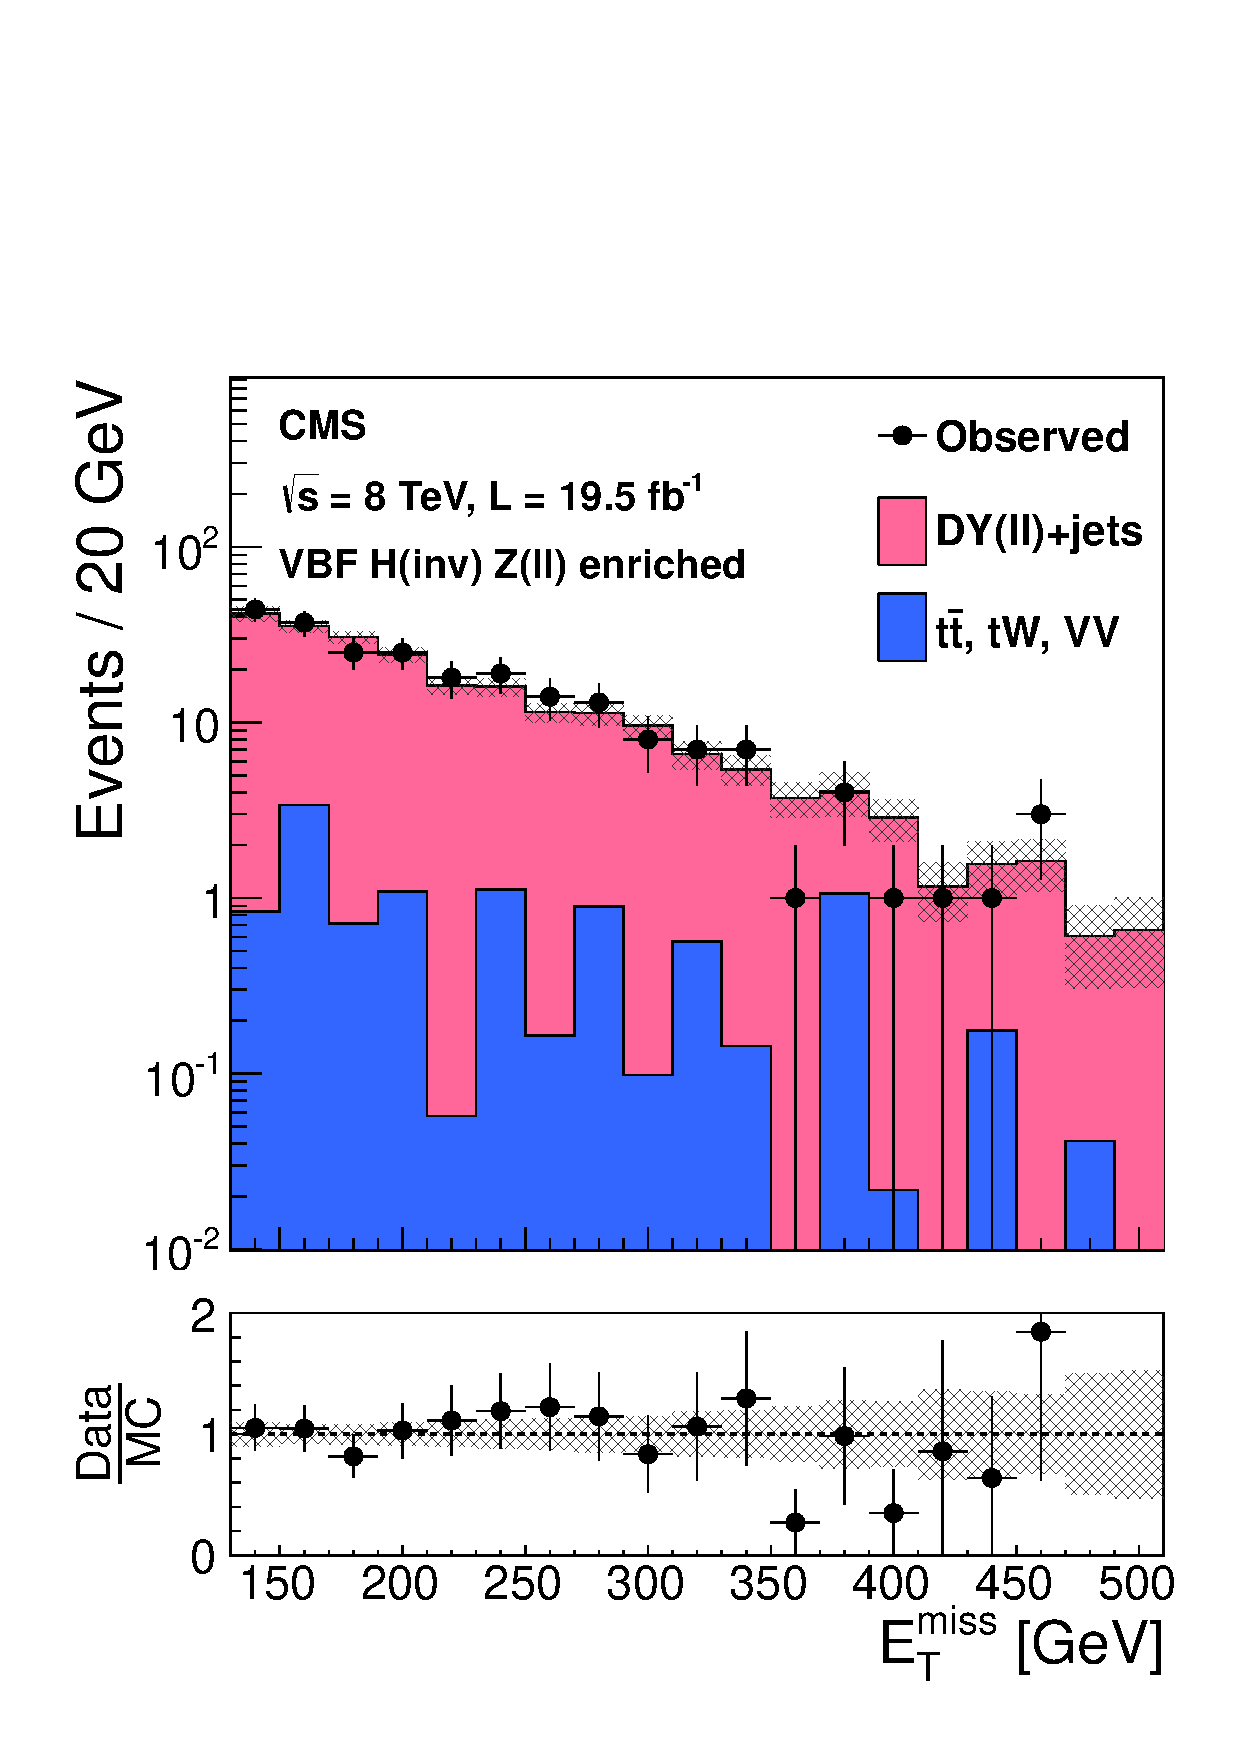
\includegraphics[width=.65\largefigwidth]{plots/prompt/VBF-ZCtrl-MET.pdf}}
  \subfloat[]{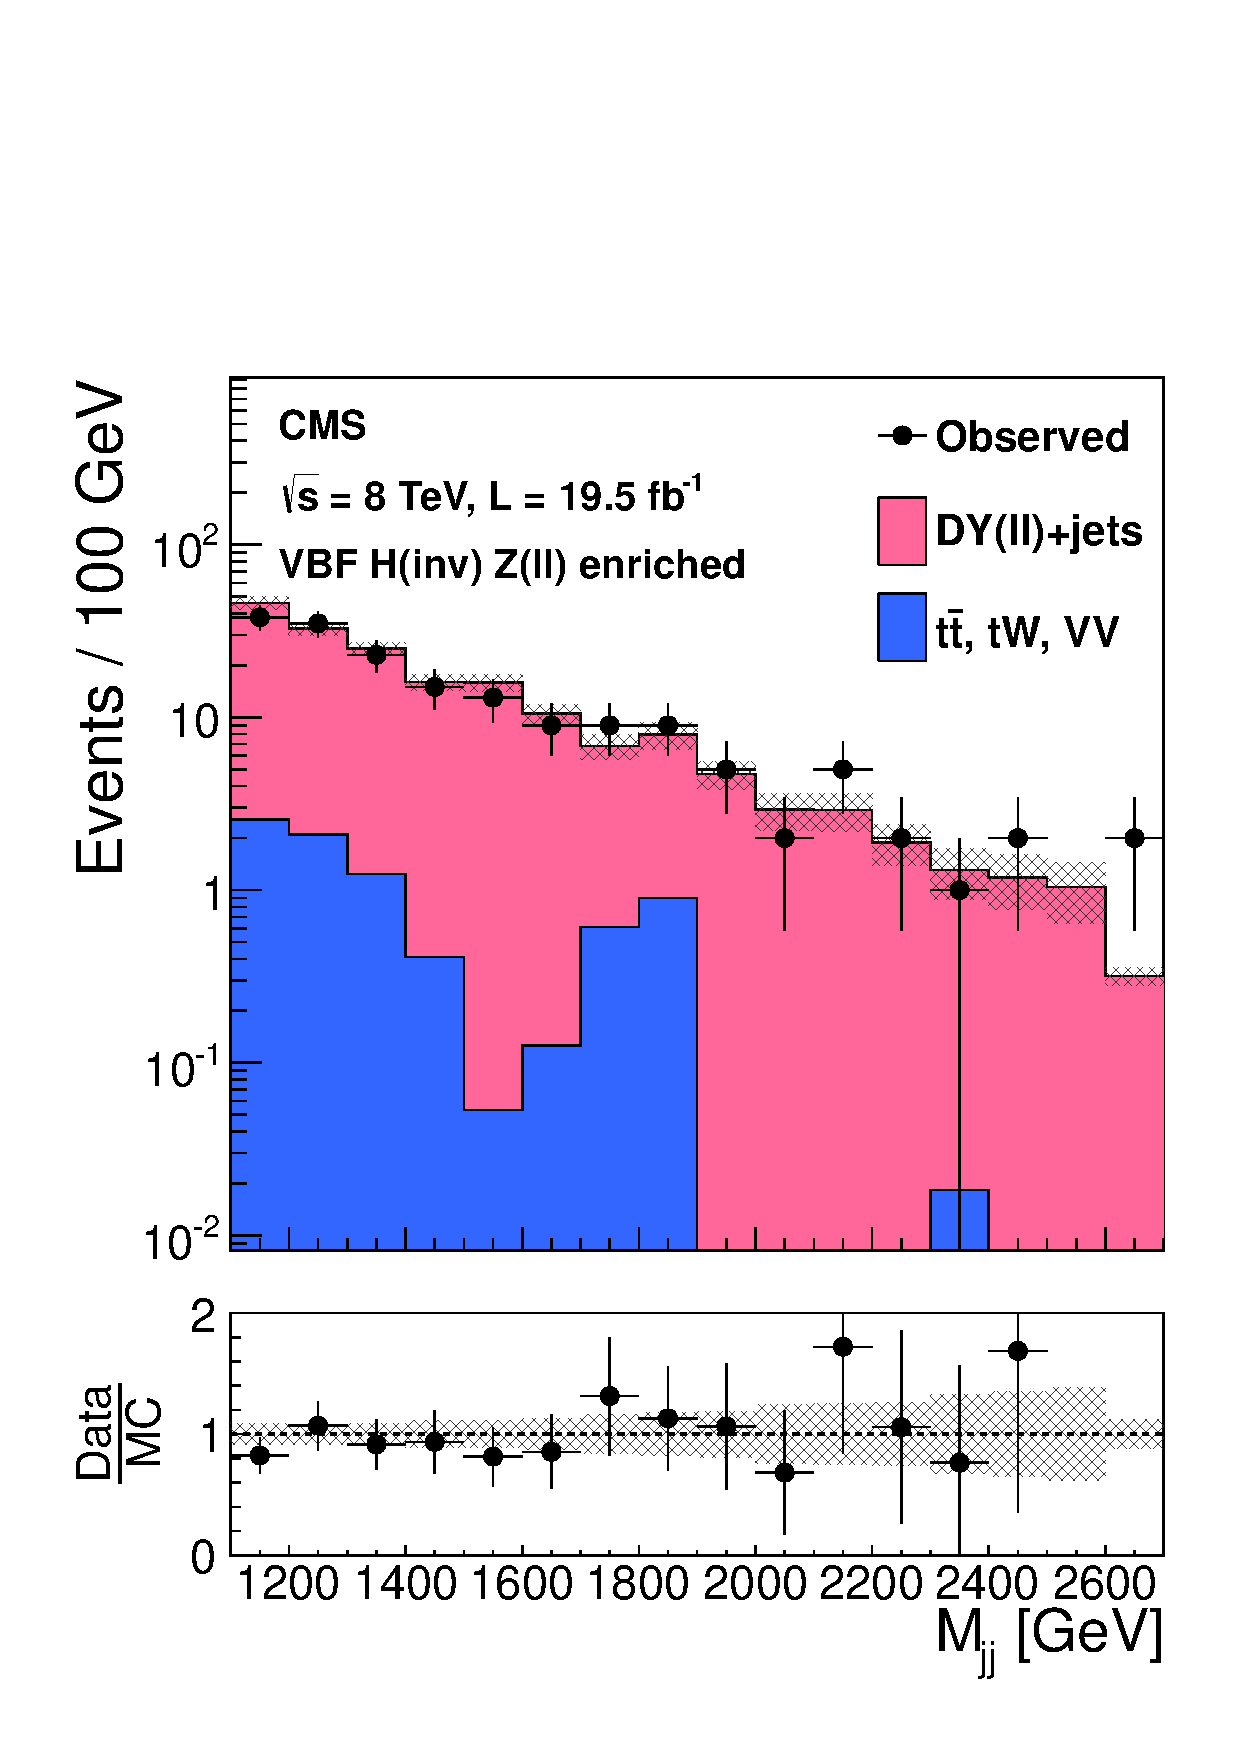
\includegraphics[width=.65\largefigwidth]{plots/prompt/VBF-ZCtrl-Mjj.pdf}}
  \DIFdelbeginFL %DIFDELCMD < \caption{%%%
\DIFdelendFL \DIFaddbeginFL \caption[Distributions of the \METnoMU (a) and \Mjj (b) in a relaxed \PZ control region, with no requirement on \dphijj, the CJV removed, and the requirements on \Mjj and \detajj relaxed to 1000 \GeV and 3.5 respectively. DY(ll)+jets indicates the contribution from Z+jets processes and $t\bar{t}$, $t\PW$, VV indicates the contribution from minor backgrounds. The hatched region illustrates the systematic uncertainty.]{\DIFaddendFL Distributions of the \METnoMU (a) and \Mjj (b) in a relaxed \PZ control region, with no requirement on \dphijj, the \DIFdelbeginFL %DIFDELCMD < \ac{CJV} %%%
\DIFdelendFL \DIFaddbeginFL \DIFaddFL{CJV }\DIFaddendFL removed, and the requirements on \Mjj and \detajj relaxed to 1000 \GeV and 3.5 respectively. DY(ll)+jets indicates the contribution from Z+jets processes and $t\bar{t}$, $t\PW$, VV indicates the contribution from minor backgrounds. The hatched region illustrates the systematic uncertainty~\cite{Chatrchyan:2014tja}.}
  \label{fig:promptznunu}
\end{figure}




\subsection{QCD}
\label{sec:promptacQCD}
The \ac{QCD} background remaining after the full event selection is mostly from events where jets are mismeasured. The size of the \ac{MC} samples available for studying this process is not sufficient for them to be relied upon for extrapolation from a control region to the signal region. The remaining \ac{QCD} background is therefore estimated using a so-called ``ABCD'' method. In this method four regions, A, B, C and D, are defined according to whether events pass or fail the \METnoMU and \ac{CJV} cuts\DIFaddbegin \DIFadd{, }\DIFaddend as shown in \FigureRef{fig:abcdmethod}. Region D is the signal region and regions A, B and C are three mutually exclusive control regions.

\begin{figure}
  \begin{tabular}{l|c|c|l}
    \multicolumn{1}{c}{}&\multicolumn{1}{c}{Fail \METnoMU} & \multicolumn{1}{c}{Pass \METnoMU} &\\
    \cline{2-3}
    Fail \ac{CJV} &\cellcolor{orange} A & \cellcolor{orange}B &\\
    \cline{2-3}
    Pass \ac{CJV} &\cellcolor{orange} C & \cellcolor{green}D &\\
    \cline{2-3}
  \end{tabular}

  \caption{A diagram of the regions used in the \DIFdelbeginFL %DIFDELCMD < \ac{QCD} %%%
\DIFdelendFL \DIFaddbeginFL \DIFaddFL{QCD }\DIFaddendFL ABCD background estimation method. Region D is the signal region and regions A, B and C are mutually exclusive control regions.}
  \label{fig:abcdmethod}
\end{figure}

The efficiency to pass the \METnoMU and \ac{CJV} cuts can be determined from the ratios between regions A and B, and A and C respectively. The number of events expected in the signal region is then:
\begin{align}
  \label{eq:abcd}
  \begin{split}
  N_{D}&=N_{A}\cdot\frac{N_{B}}{N_{A}}\cdot\frac{N_{C}}{N_{A}}\\
  &=\frac{N_{B}\cdot N_{C}}{N_{A}},
  \end{split}
\end{align}
where $N_{A,B,C}$ is the number of events observed in region $A,B,C$ in data minus the number expected from V+jets or other minor backgrounds, i.e. the number of events in the region believed to be from QCD. This method relies on the probability of an event passing the \ac{CJV} being uncorrelated with the \METnoMU of the event. This has been checked by comparing the \METnoMU distribution, below the 130 \GeV signal region requirement, for events which pass and fail the \ac{CJV} \DIFaddbegin \DIFadd{(see }\FigureRef{prompt:qcdmetcjv}\DIFadd{)}\DIFaddend . The maximum fractional difference observed between bins of these two distributions is 40\%, so this is added as a systematic to the \ac{QCD} background yield. The method was also tested in a region orthogonal to the signal region with all requirements the same as those of the signal region except \dphijj which was required to be greater than 2.6. In this test region, which is expected to be \ac{QCD} dominated, the \DIFdelbegin \DIFdel{prediction }\DIFdelend \DIFaddbegin \DIFadd{observation }\DIFaddend agreed with the expectation within 15\%, which is within the systematic uncertainty assigned to the method. The results of using this method to estimate the number of QCD events in the signal region are shown in \TableRef{tab:promptqcd}.

\begin{figure}
  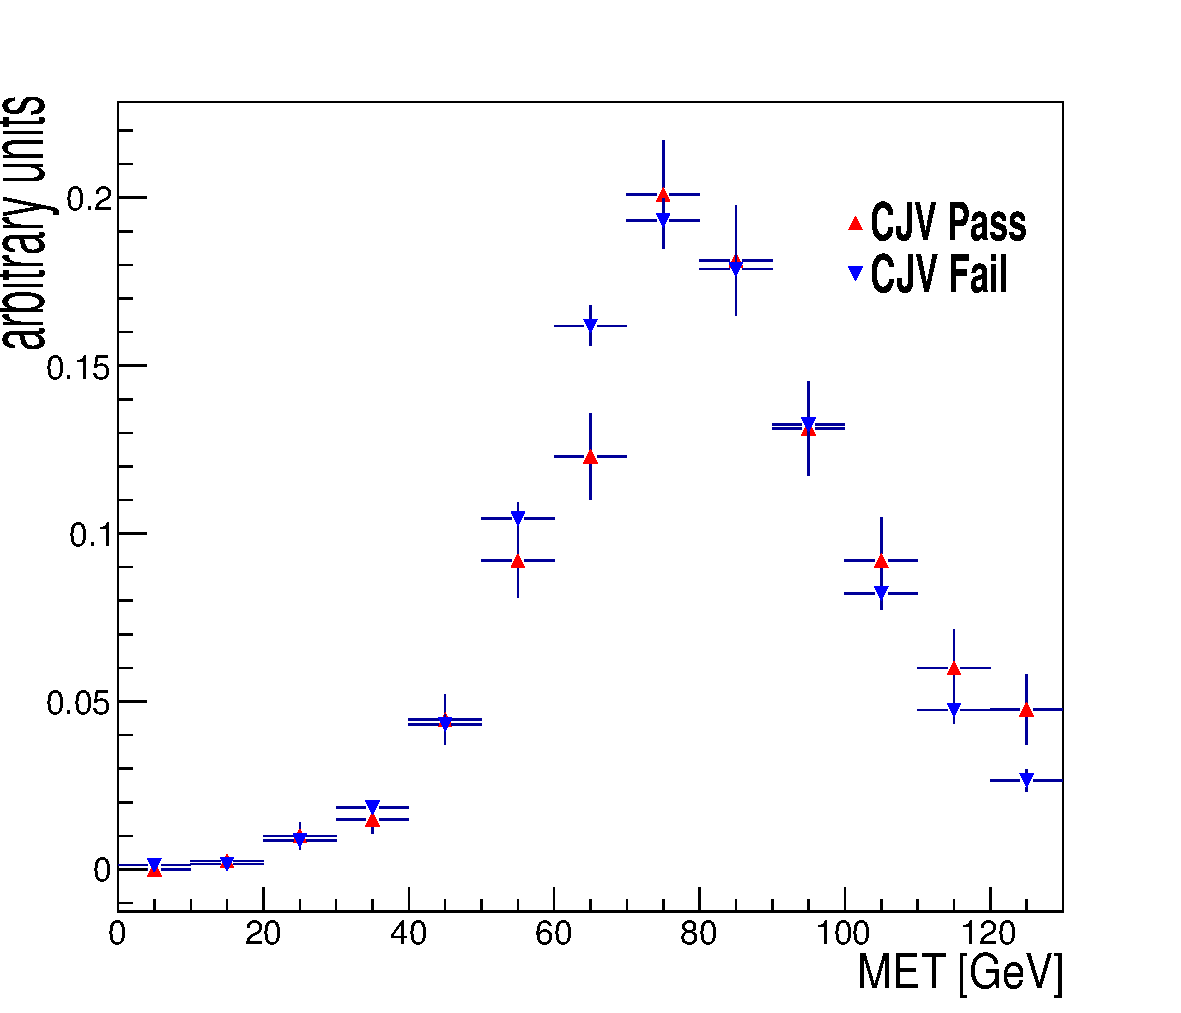
\includegraphics[width=1.2\largefigwidth]{plots/prompt/AN-12-403-figs/QCD3_CtrlLo_MET.pdf}
  \caption{Distribution of the \METnoMU for events passing and failing the \DIFdelbeginFL %DIFDELCMD < \ac{CJV}%%%
\DIFdelendFL \DIFaddbeginFL \DIFaddFL{CJV}\DIFaddendFL . \DIFaddbeginFL \DIFaddFL{Both distributions are normalised to a total integral of 1. }\DIFaddendFL The largest difference seen in any bin is 40\%. This difference is used to assign as a systematic uncertainty on the \DIFdelbeginFL %DIFDELCMD < \ac{QCD} %%%
\DIFdelendFL \DIFaddbeginFL \DIFaddFL{QCD }\DIFaddendFL background estimation.}
  \label{prompt:qcdmetcjv}
\end{figure}

%Table of results
\begin{table}
  \caption{Numbers of events from data and \DIFdelbeginFL %DIFDELCMD < \ac{MC} %%%
\DIFdelendFL \DIFaddbeginFL \DIFaddFL{MC }\DIFaddendFL in each region used in the \DIFdelbeginFL %DIFDELCMD < \ac{QCD} %%%
\DIFdelendFL \DIFaddbeginFL \DIFaddFL{QCD }\DIFaddendFL background estimate and the final estimated number of events.}
  \label{tab:promptqcd}
  \begin{tabular}{lccc}
    \hline
    \hline
    Region & Data & Background & Data-Background \\
    \hline
    \hline
    $N_{A}$ & 5118 & $222\pm 14$ & $4896\pm 73$\\
    $N_{B}$ & 773  & $586\pm 17$ & $184 \pm 33$\\
    $N_{C}$ & 896  & $76.9\pm 8.3$ & $819\pm 31$\\
    \hline
    $N_{D}$ & - & - & \textcolor{red}{$30.9\pm 1.6$}\\
    \hline
    \hline
  \end{tabular}
\end{table}

\subsection{Minor backgrounds}
\label{sec:promptminor}
In addition to the V+jets and QCD backgrounds which account for 94\% of the expected events in the signal region, there is also a small number of events expected from other minor backgrounds including single top quark production, top quark pair production, diboson production and \Zmumu. Due to their small contributions these numbers of events are taken directly from \ac{MC}. The diboson backgrounds are simulated using \textsc{Pythia 6}, the single top quark background using \textsc{Powheg} and the top quark pair production and $\PZ/\gamma^{*}\rightarrow\ell\ell$ backgrounds using \textsc{MadGraph}. The cross-sections used to normalise these \ac{MC} samples were taken from the most \DIFdelbegin \DIFdel{up to date }\DIFdelend \DIFaddbegin \DIFadd{up-to-date }\DIFaddend CMS published results at the time of the analysis~\cite{CMS:2012fza,CMS:2012iza,CMS:2012zva,CMS:2013qea,CMS:2013hea}. The final estimate of the number of events from minor backgrounds in the signal region is $20\pm 8.2$(MC stat), with 70\% of these expected to be from diboson production.


\section{Systematic uncertainties}
\label{sec:promptsyst}
The dominant uncertainties in the analysis are the statistical uncertainties on the V+jets backgrounds due to the number of data events observed in the control regions. In addition, as well as those mentioned in \SectionRef{sec:promptbkg}, there are several further systematic uncertainties on the expected numbers of signal and background events. These uncertainties are described individually below and the fractional uncertainty on the total expected number of signal and background events from all sources of uncertainty are summarised in \TableRef{tab:promptsysts}.
\subsection{Jet energy scale}
\label{sec:promptjes}
The reconstructed energy of a jet reconstructed by CMS is not necessarily the same as the true energy of all the particles that make it up. As described in \SectionRef{sec:jec}, jet corrections are applied to remedy this. The correction for the ratio between reconstructed and true jet energy is referred to as the \ac{JES}. Uncertainties on the \ac{JES} come from several sources. The \ac{JES} obtained from the dijet \pt balance method for instance has an uncertainty from the jet resolution bias~\cite{CMS-JME-10-011}. This bias arises because the jet \pt spectrum sharply falls with increasing \pt. Such a spectrum leads to the well measured jet being used as the base for the balance method \DIFdelbegin \DIFdel{to be }\DIFdelend \DIFaddbegin \DIFadd{being }\DIFaddend more likely to have fluctuated up in \pt than down. The main uncertainties in the photon/\PZ balance methods come from the limited number of events in the samples used. The \ac{JES} obtained in \ac{MC} is also different when measured with different \ac{MC} generators, which leads to an uncertainty.

These uncertainties on the \ac{JES} give rise to an uncertainty on the energy of all jets in CMS events. The impact of this uncertainty on the expected and observed event yields in this analysis was estimated \DIFdelbegin \DIFdel{be }\DIFdelend \DIFaddbegin \DIFadd{by }\DIFaddend altering the \ac{JES} correction up by one standard deviation, ``JESUP'', and down by one standard deviation ``JESDOWN'', and recalculating the energy and momentum of all jets in each event. The \MET is recalculated taking into account the updated jet energies. Furthermore, as the jet energy scale uncertainty varies with \pt and $\eta$, it is possible for the \pt ordering of the jets to change when the \ac{JES} is changed. The \ac{VBF} tag pair is therefore \DIFdelbegin \DIFdel{rechosen }\DIFdelend \DIFaddbegin \DIFadd{chosen again, so as }\DIFaddend to be the new highest \pt pair of jets. 

After modifying the \ac{JES}, the analysis is \DIFdelbegin \DIFdel{reperformed }\DIFdelend \DIFaddbegin \DIFadd{performed again }\DIFaddend and the resulting change in the expected signal and background yields is taken to be the uncertainty due to the \ac{JES}. The sub-leading jet's \pt in a W+jets \ac{MC} sample is shown for the nominal \ac{JES}, JESUP and JESDOWN in \FigureRef{fig:promptjes}. It can be seen that altering the \ac{JES} results in a smooth change in the jet \pt, indicating that the difference in the number of events passing the analysis cuts is not due to individual events with large weights migrating in and out of the signal region.

%plot from AN-13-205
\begin{figure}
  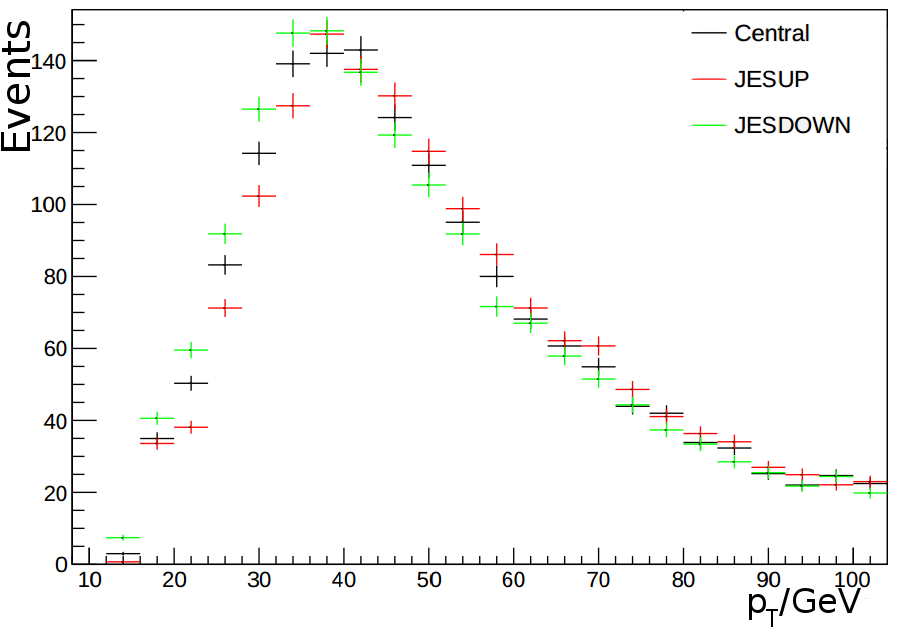
\includegraphics[width=\largefigwidth]{plots/prompt/jescheckzoom.png}
  \caption{The distribution of the sub-leading jet's \pt in W+Jets \DIFdelbeginFL %DIFDELCMD < \ac{MC} %%%
\DIFdelendFL \DIFaddbeginFL \DIFaddFL{MC }\DIFaddendFL events with the nominal \DIFdelbeginFL %DIFDELCMD < \ac{JES} %%%
\DIFdelendFL \DIFaddbeginFL \DIFaddFL{JES }\DIFaddendFL and for JESUP and JESDOWN.}
  \label{fig:promptjes}
\end{figure}

\subsection{Jet energy resolution}
\label{sec:promptjer}
The width of the jet energy distribution, the \ac{JER}, differs between \ac{MC} and data. This is partly due to \ac{MC} samples being generated before and during data taking, and thus before a measurement of the exact resolution in data can be performed. Measuring the \ac{JER} in data is done in a very similar way to the measurement of the \ac{JES} using dijet and photon/\PZ-jet balance techniques and by comparing the reconstructed energy to that generated in \ac{MC}, and thus has the same sources of uncertainty.

To correct the \ac{MC} resolution to match that in the data, the \pt of all jets in \ac{MC} is ``smeared''. The smearing is carried out using two methods. The first method is used for jets in \ac{MC} that are within 0.5 in the $\eta-\phi$ plane of a generator jet. In this method the difference between the reconstructed and generator jet \pt is scaled by a correction factor, $c$, chosen to be the ratio between the resolution of the data and \ac{MC} and calculated as a function of the jet's \pt and $\eta$. The resulting jet \pt is given by:
\begin{equation}
  \label{eq:promptjermatched}
  \pt'=\rm{max}\left[0,\mathnormal{p}_{{\mathrm{T}}gen}+\DIFdelbegin \DIFdel{c}\DIFdelend \DIFaddbegin \DIFadd{\mathit{c}}\DIFaddend \left(\mathnormal{p}_{\mathrm{T}}-\mathnormal{p}_{{\mathrm{T}}gen}\right)\right],
\end{equation}
where \pt is the initial transverse momentum, $\pt'$ is the transverse momentum after smearing and $p_{\mathrm{T}gen}$ is the matched generator jet's \pt. This procedure has the advantage that the smearing is not reliant on random factors and is therefore reproducible, making synchronisation between analysis implementations easier. \DIFaddbegin \DIFadd{The factor $c$ depends on the }\pt \DIFadd{and $\eta$ of the jet and is calculated so as to represent the average resolution over the whole 2012 run period. 
}\DIFaddend 

The second method is used when a jet has no matching generator jet. In this case a random correction is necessary. The technique used is to add a fluctuation to the jet's \pt with a size obtained by sampling a gaussian with width:
\begin{equation}
  \label{eq:promptjerunmatched}
  \sqrt{\left(c^{2}-1\right)\sigma_{MC}},
\end{equation}
where $c$ is the same correction factor from the method above and $\sigma_{MC}$ is the initial \ac{MC} resolution as a function of \pt and $\eta$. $\sigma_{MC}$ was measured by performing a gaussian fit to the distribution of the ratio between the generator-level and offline jet \pt observed in $\PW+$jets \ac{MC}. As well as being random and thus difficult to reproduce, this method has the disadvantage that it can only be used to worsen the resolution. 

The analysis is performed three times with three different smearings, one where the MC resolution is smeared to match the nominal data resolution, which is used for the main signal and background estimations, and two where the \ac{MC} resolution is made to match the improvement, ``JERBETTER'' and worsening, ``JERWORSE'' of the jet energy resolution by one standard deviation. For the nominal \DIFdelbegin \DIFdel{and JERWORSE }\DIFdelend \DIFaddbegin \DIFadd{resolution $c-1$ varies from less than 1}\% \DIFadd{in the central region, to 9}\% \DIFadd{in the }\ac{HF}\DIFadd{, while for ``JERBETTER'' and ``JERWORSE'' it varies from 10}\% \DIFadd{in the central region of the detector to 49}\% \DIFadd{in the }\ac{HF}\DIFadd{. In the case of the nominal and JERWORSE }\DIFaddend smearings the limitation that the unmatched jet smearing method can only worsen the resolution is not a problem, as the initial \ac{MC} resolution is better than that in data for all values of jet \pt and $\eta$. However, for the JERBETTER smearing it is necessary to improve the resolution for some jets. Fortunately, the differences between the generated resolution and the JERBETTER resolutions where improved resolution is required are small, so in these cases no smearing is applied. For all smearings the resulting changes in jet \pt are propagated through to the \MET. The differences between the signal and background yields obtained with the nominal \ac{JER}, JERBETTER and JERWORSE are used to assign an uncertainty due to the \ac{JER}.

\subsection{Unclustered energy scale}
\label{sec:promptues}
In addition to the uncertainties on the \MET from the propagation of \ac{JES} and \ac{JER} uncertainties there are also uncertainties from the other elements contributing to the \MET. Electrons and muons contribute to the \MET, but have very good resolution and small scale uncertainties compared to jets so their contribution to the \MET uncertainty is considered negligible~\cite{CMS-PAS-JME-12-002}. Unclustered energy, which is made up of all of the energy deposits in the calorimeters not identified as part of an object, such as a jet or lepton, still contributes to the \MET, and has a non-negligible scale uncertainty~\cite{CMS-PAS-JME-12-002}. %citation

The \ac{UES} is measured using photon and \PZ events with jets present in them, where it can be assumed that the \MET should be zero~\cite{CMS-PAS-JME-12-002}. After jet energy corrections, the distribution of the remaining difference between the photon or \PZ momentum and the jets is therefore centered around zero, and its width can be taken as the uncertainty on the \ac{UES}. The \ac{UES} in all events is modified up and down by this uncertainty and the \MET recalculated. The differences in the obtained signal and background event yields obtained through this process are used as the uncertainty from this source.

\subsection{Lepton identification and isolation efficiency}
\label{sec:promptlepweights}
As described in \SectionRef{sec:mcweights} \ac{MC} events are reweighted using scale factors to account for differences in the electron and muon identification and isolation efficiency. The weights due to these efficiencies are varied up and down by the uncertainties from the tag and probe method used to measure them, and the difference in the resulting signal and background yield used as the uncertainty from this source.

An uncertainty of 8\% is added to the estimate of the $\PW\rightarrow\tau\nu$ background to account for the uncertainty in the tau identification efficiency, which is measured using $\PZ\rightarrow\tau\tau$ events where one tau decays to a muon and the other hadronically~\cite{Chatrchyan:1385560}. 5\% of events in the $\PW\rightarrow\tau\nu$ control region also appear to be due to $\PW\rightarrow e\nu$ events where the electron or a jet has been misreconstructed as a tau, so a further 5\% systematic is assigned to the $\PW\rightarrow\tau\nu$ estimate.


\subsection{Other uncertainties}
\label{sec:promptzextrap}
Additional uncertainties arise from several sources. For instance, the \Znunu background estimate is reliant on the ratio of the cross-sections for the \Znunu and \Zmumu processes in the phase space of this analysis. A 20\% uncertainty on this ratio was applied to cover the difference between the values of the ratio calculated using \textsc{MadGraph} and using \textsc{MCFM}~\cite{ARTICLE:CMSAN-12-403}. Further uncertainties come from the measurement of the distribution of the number of primary vertices used in the pileup weights, described in \SectionRef{sec:mcweights}, the \ac{PDF}s and \ac{QCD} scale used in the signal cross-section measurements~\cite{Dittmaier:2011ti,Dittmaier:2012vm}, differences in the \ac{ggH} \dphijj spectrum depending on the \ac{MC} generator used~\cite{ARTICLE:CMSAN-12-403}, the cross-sections used to normalise the minor backgrounds, described in \SectionRef{sec:promptminor}, and the measurement of the total integrated luminosity~\cite{CMS-PAS-LUM-13-001}.


\begin{table}
  \caption{A summary of the uncertainties in the total expected signal and background yields. All uncertainties are quoted as the percentage change in the yield when each effect is varied up and down according to its uncertainty. The signal yields assume a Higgs boson mass of 125\GeV.}
  \label{tab:promptsysts}
  \begin{tabular}{lcc}
    \hline
    \hline
    Uncertainty source & Total background & Signal \\
    \hline
    Control region statistics               & 11\%          & \NA  \\
    MC statistics and \Znunu cross-section ratio  & 11\%          & 4\%  \\
    \ac{JES}, \ac{JER} and \ac{UES}         & 7\%           & 13\% \\
    QCD background estimation               & 4\%           & \NA  \\
    Lepton efficiency                       & 2\%           & \NA  \\
    Luminosity                              & 0.2\%         & 2.6\%\\
    Cross-sections                          & 0.5--1\%      & \NA  \\
    PDFs                                    & \NA           & 5\%  \\
    \ac{QCD} scale     & \NA           & 4\%  \\
    \ac{ggH} \dphijj spectrum           & \NA           & 4\%  \\
    \hline
    Total & 18\% & 14\% \\
    \hline
    \hline
  \end{tabular}
\end{table}

\section{Results}
\label{sec:promptresults}
The final results of all the background estimation methods and systematic uncertainty studies are summarised in \TableRef{tab:promptresults}. The total number of events expected from background processes in the signal region is $332\pm 46\stat\pm 45\syst$. The presence of a Higgs boson with a mass of 125 \GeV, \ac{SM} production and \BRinv$=100\%$ would be expected to yield $224\pm 31$  signal events\DIFdelbegin \DIFdel{would be expected}\DIFdelend , with 6\% of these from \ac{ggH} and the remainder from \ac{VBF} production. 390 events are observed, which is within one standard deviation of the \DIFdelbegin \DIFdel{background only }\DIFdelend \DIFaddbegin \DIFadd{background-only }\DIFaddend prediction. \FigureRef{fig:promptresults} shows the \METnoMU and \Mjj of the background and signal events expected, and the data observed, in the signal region. 

%table of yields
\begin{table}
  \caption{The estimated numbers of background and signal events, together with the observed yield, in the signal region. The signal yield assumes a Higgs boson mass of 125 \GeV and \BRinv$=100\%$.}
  \label{tab:promptresults}
  \begin{tabular}{lc}
    \hline
    \hline
    Process & Event yield \\
    \hline
    \hline
    \Znunu & $99\pm 29\stat\pm 25\syst$ \\
    $\PW\rightarrow e\nu$ & $67\pm 5\stat\pm 16\syst$ \\
    $\PW\rightarrow\mu\nu$ & $63\pm 9\stat\pm 18\syst$ \\
    $\PW\rightarrow\tau\nu$ & $53\pm 18\stat\pm 18\syst$ \\
    QCD multijet & $31\pm 5\stat\pm 23\syst$ \\
    Minor backgrounds & $20\pm 8\syst$\\
    \hline 
    Total background & $332\pm 36\stat\pm 45\syst$ \\
    \hline
    \ac{VBF} H(inv.) & $210\pm 29\syst$ \\
    \ac{ggH}(inv.) & $14\pm 10\syst$ \\
    \hline 
    \hline
    Observed data & $390$ \\
    \hline
  \end{tabular}
\end{table}

%distributions
\begin{figure}
  \subfloat[]{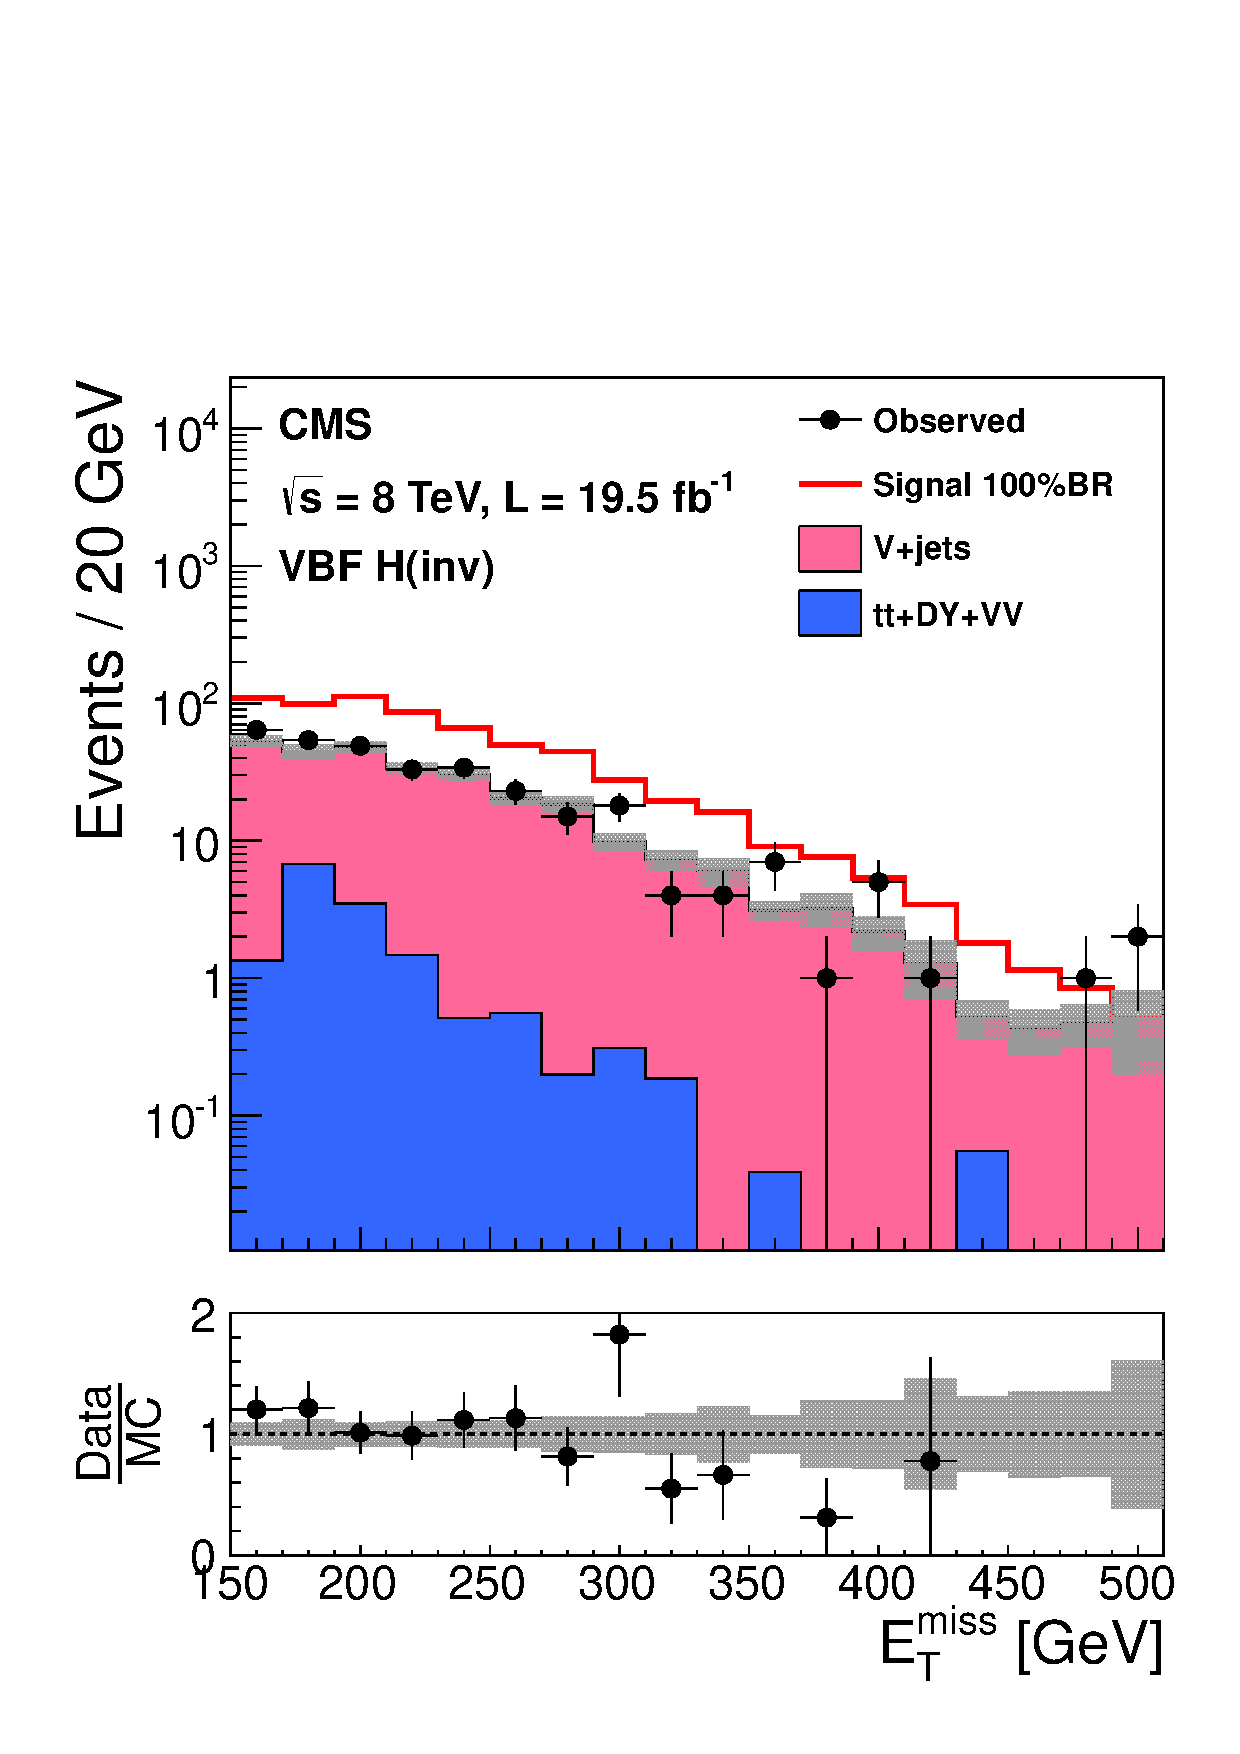
\includegraphics[width=.65\largefigwidth]{plots/prompt/AN-12-403-figs/SignalRegionMET.pdf}}
  \subfloat[]{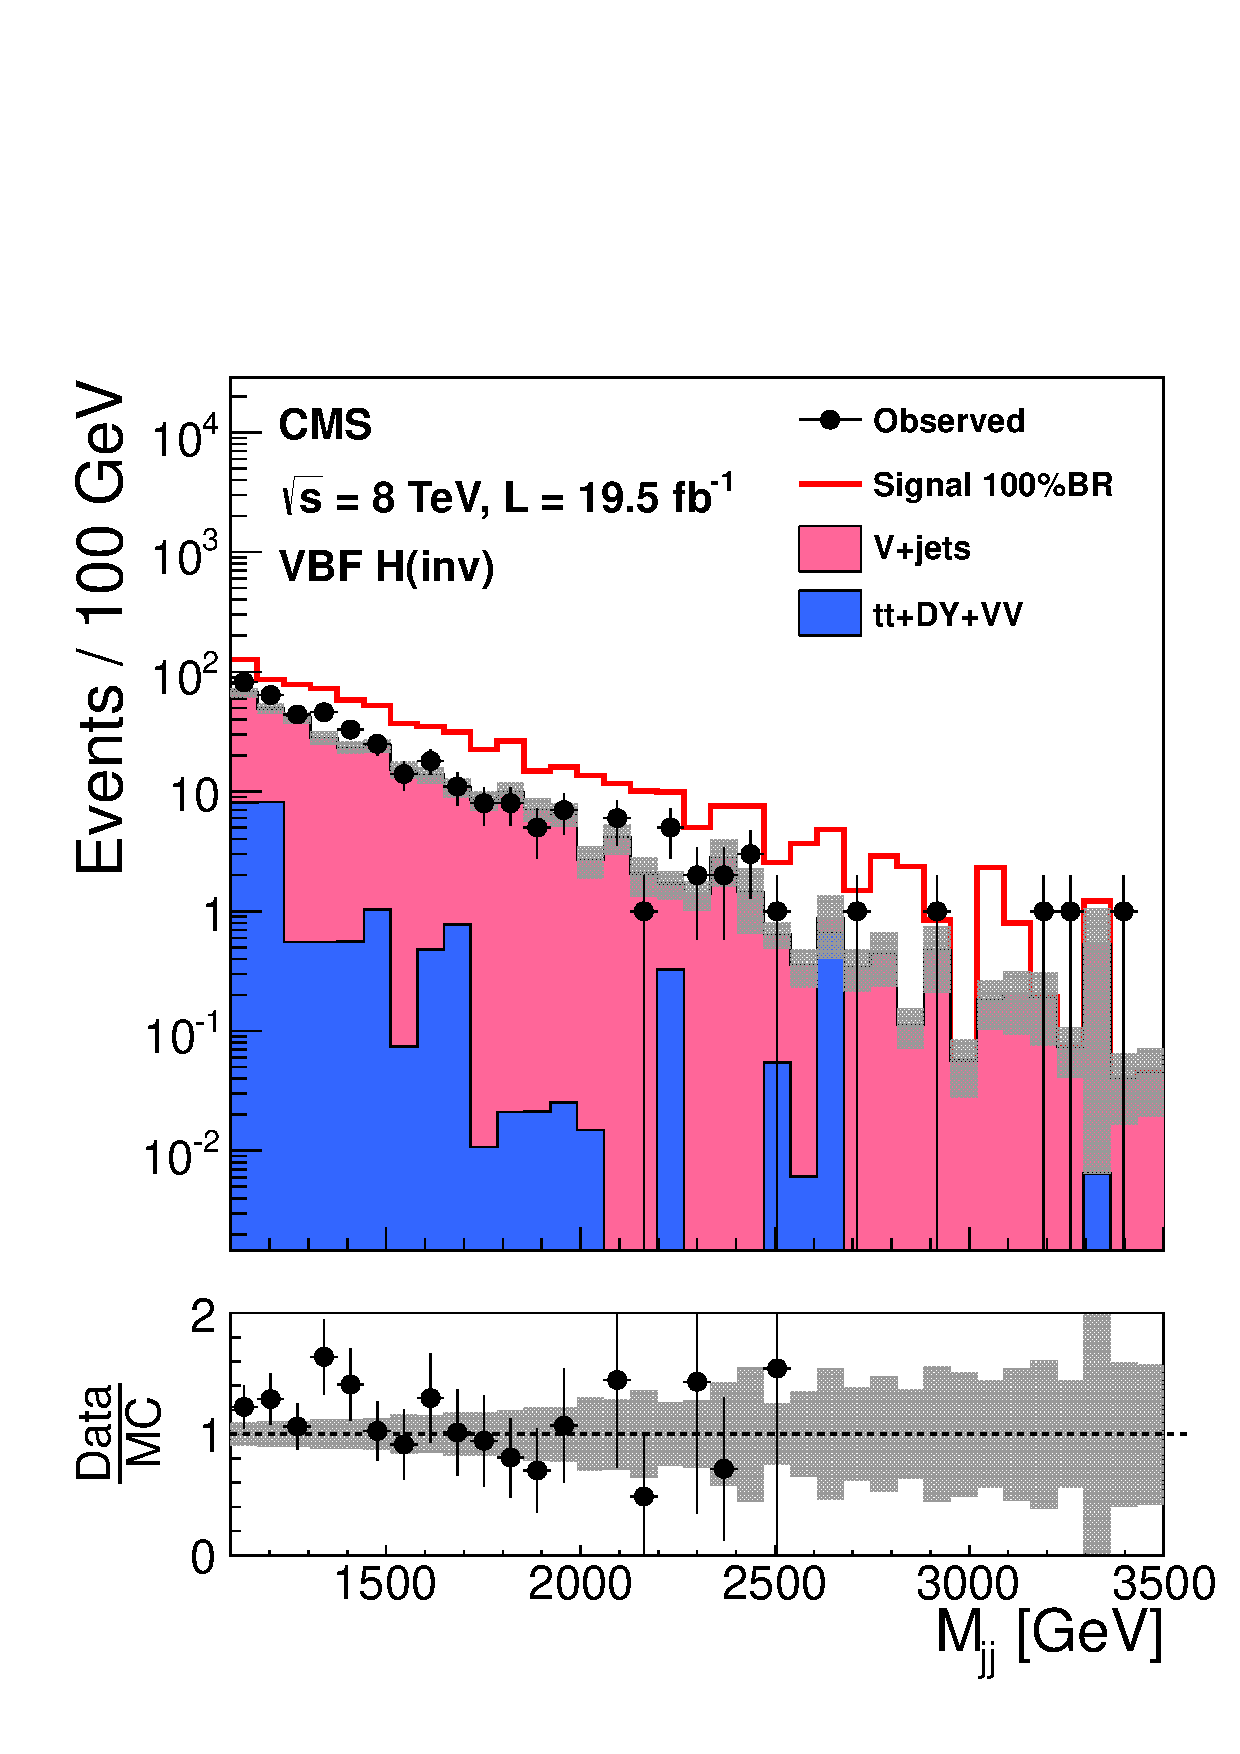
\includegraphics[width=.65\largefigwidth]{plots/prompt/AN-12-403-figs/SignalRegionMjj.pdf}}
  \DIFdelbeginFL %DIFDELCMD < \caption{%%%
\DIFdelendFL \DIFaddbeginFL \caption[Distributions of the \METnoMU (a) and \Mjj (b) of events observed in data and expected from the background estimation methods described in \SectionRef{sec:promptbkg} in the signal region. tt+DY+VV indicates the contribution from minor backgrounds. The hatched region illustrates the systematic uncertainty. The QCD background is not shown due to the very low number of events in the MC samples. The cumulative effect of a signal from a Higgs boson with mass of 125 \GeV, decaying 100\% to invisible final states is also shown.]{\DIFaddendFL Distributions of the \METnoMU (a) and \Mjj (b) of events observed in data and expected from the background estimation methods described in \SectionRef{sec:promptbkg} in the signal region. tt+DY+VV indicates the contribution from minor backgrounds. The hatched region illustrates the systematic uncertainty. The QCD background is not shown due to the very low number of events in the \DIFdelbeginFL %DIFDELCMD < \ac{MC} %%%
\DIFdelendFL \DIFaddbeginFL \DIFaddFL{MC }\DIFaddendFL samples. The cumulative effect of a signal from a Higgs boson with mass of 125 \GeV, decaying 100\% to invisible final states is also shown~\cite{Chatrchyan:2014tja}.}
  \label{fig:promptresults}
\end{figure}

As no excess is observed, the asymptotic $CL_{S}$ technique, described in \SectionRef{sec:stats}, is used to place an upper limit on the production cross-section times branching fraction, $\sigma\times\mathcal{B}$, at 95\% \ac{CL}. Under the assumption of \ac{SM} production this limit can be interpreted as a limit on \BRinv. All systematic uncertainties are modelled as log-normally distributed nuisance parameters, with the exception of the statistical uncertainty on the $Z\rightarrow\nu\nu$ background, which is modelled as a gamma-normally distributed nuisance due to the low number of events in the dimuon control region. A gamma-normal distribution is used in the case of control regions with low numbers of events because in this case the central limit theorem does not apply so the Poisson probability of observing a certain number of events is very asymmetric; this asymmetry is well modelled by a gamma-normal distribution~\cite{2003sppp.conf...35L}.

The resulting upper limits are shown as a function of Higgs boson mass in \FigureRef{fig:promptlimits}, with the 95\% \ac{CL} observed (expected) limit on \BRinv for a 125 \GeV Higgs boson being 65\% (49\%). The green and yellow bands shown in \FigureRef{fig:promptlimits} denote the one and two sigma uncertainty bands respectively of the expected limit, also calculated using the asymptotic technique. The one (two) sigma band represents the region that the observation is expected to lie in 68\% (95\%) of the time if the \DIFdelbegin \DIFdel{background only }\DIFdelend \DIFaddbegin \DIFadd{background-only }\DIFaddend hypothesis is true.

This was the first published search for invisibly decaying Higgs bosons in the \ac{VBF} channel. It can be seen that for all values of Higgs boson mass investigated the observed limit is approximately one sigma above the expected limit. If the measurements of the limit at each Higgs boson mass were not correlated, this could be seen as evidence for an excess. However, as this analysis has only a single bin, and no information on the shape of the event variable distributions is used, the measurements for the different Higgs boson masses are 100\% correlated with each other. The analysis therefore sees no significant evidence of non-\ac{SM} behaviour.

%limit plots
\begin{figure}
  \subfloat[]{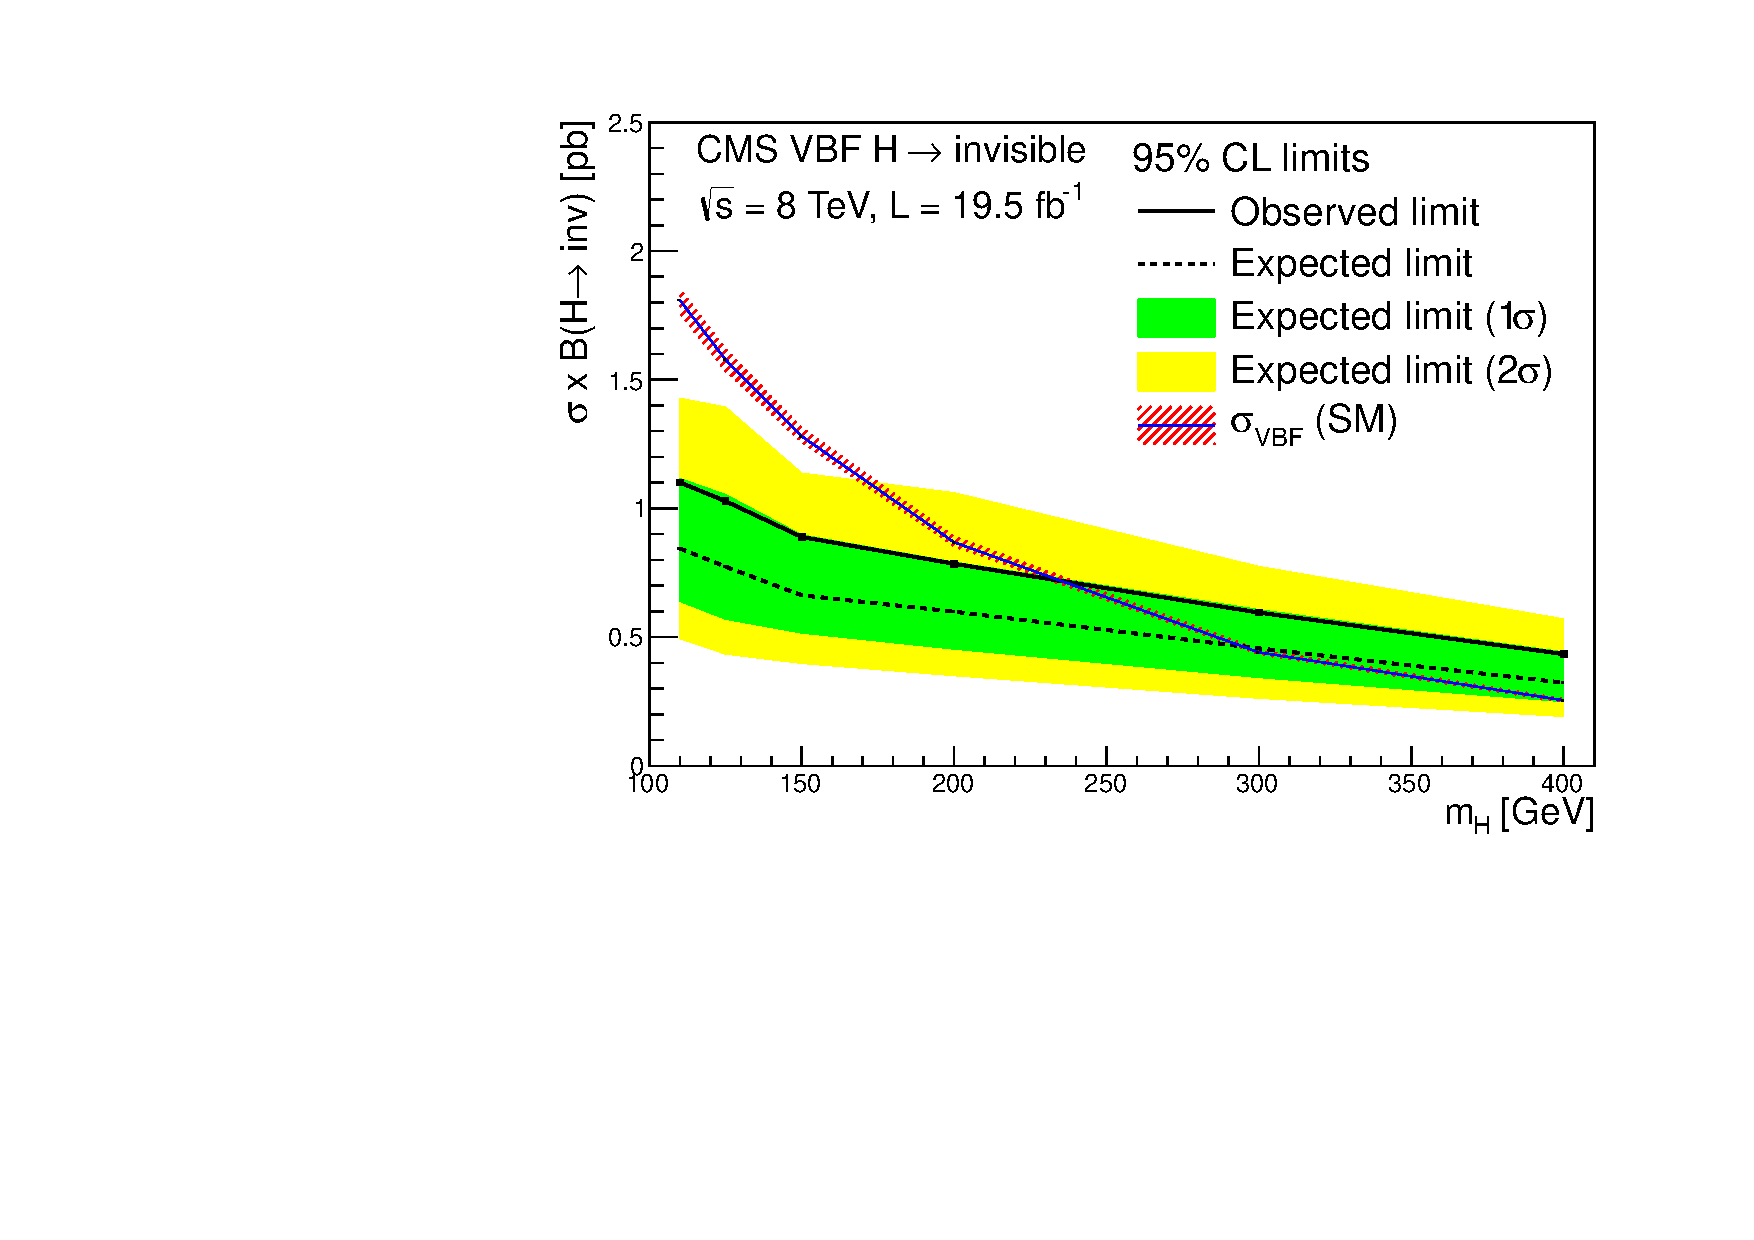
\includegraphics[width=\largefigwidth]{plots/prompt/HIG-13-30-figs/vbfxslimit.pdf}}

  \subfloat[]{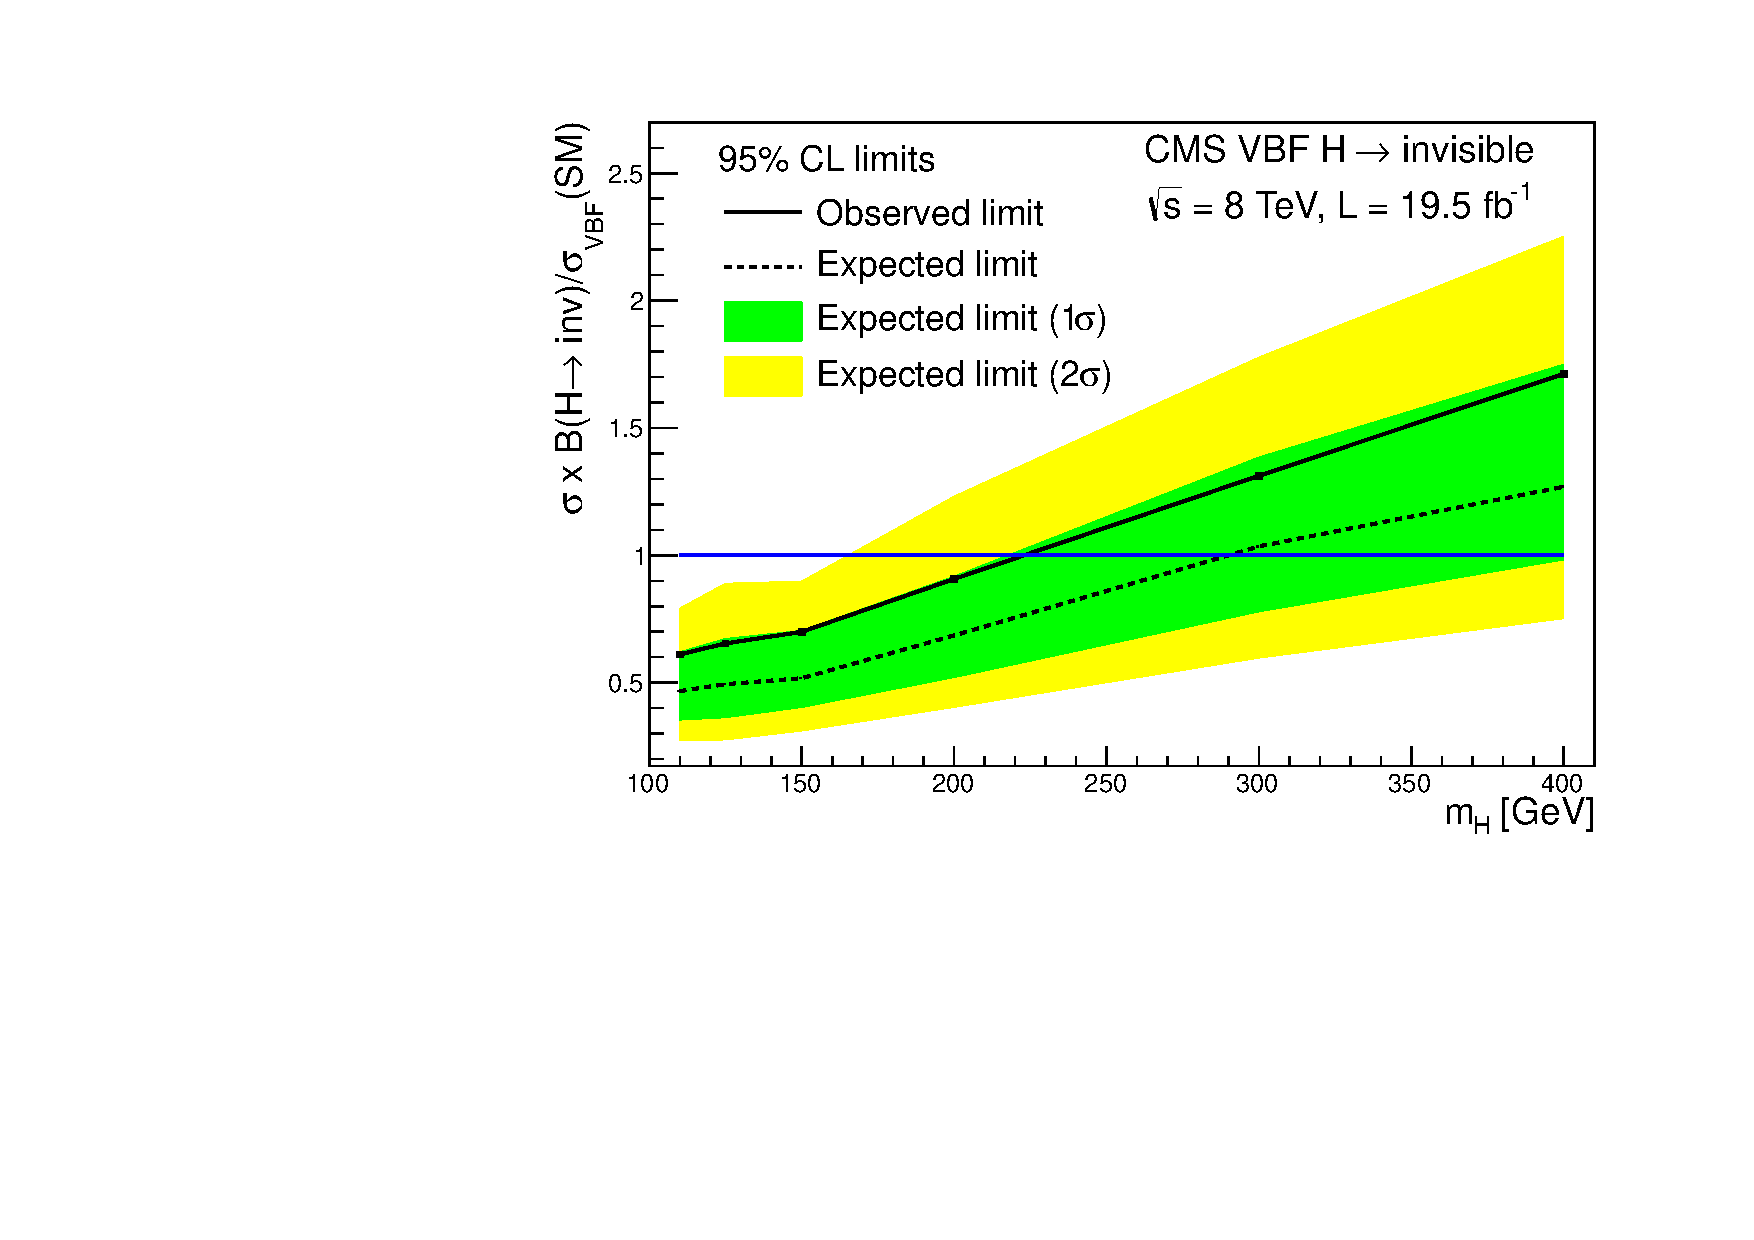
\includegraphics[width=\largefigwidth]{plots/prompt/HIG-13-30-figs/vbflimit.pdf}}
  \DIFdelbeginFL %DIFDELCMD < \caption{%%%
\DIFdelendFL \DIFaddbeginFL \caption[Expected and observed 95\% CL upper limits on the VBF $\sigma\times\mathcal{B}$ in \pb (a) and normalised to the SM VBF Higgs boson production cross-section (b). The green and yellow bands indicate the 68\% and 95\% confidence intervals on the expected limit respectively.]{\DIFaddendFL Expected and observed 95\% \DIFdelbeginFL %DIFDELCMD < \ac{CL} %%%
\DIFdelendFL \DIFaddbeginFL \DIFaddFL{CL }\DIFaddendFL upper limits on the \DIFdelbeginFL %DIFDELCMD < \ac{VBF} %%%
\DIFdelendFL \DIFaddbeginFL \DIFaddFL{VBF }\DIFaddendFL $\sigma\times\mathcal{B}$ in \pb (a) and normalised to the SM \DIFdelbeginFL %DIFDELCMD < \ac{VBF} %%%
\DIFdelendFL \DIFaddbeginFL \DIFaddFL{VBF }\DIFaddendFL Higgs boson production cross-section (b)~\cite{Chatrchyan:2014tja}. The green and yellow bands indicate the 68\% and 95\% confidence intervals on the expected limit respectively.}
  \label{fig:promptlimits}
\end{figure}
\chapter{Search for invisibly decaying Higgs bosons in Run 1 parked data}
\label{chap:parked}
The parked data, described in \SectionRef{sec:triggers}, used for this analysis was collected using a range of triggers with similar but looser requirements than those used for the prompt data (``prompt'') analysis described in the previous chapter. These looser requirements allow areas of phase space which were previously removed by the prompt trigger to be used. However, these areas also have very large \ac{QCD} backgrounds, and require the analysis selection 
and some background estimation methods to be redesigned compared to the prompt analysis. As it was reconstructed later the parked data also uses different, better, detector calibrations (such as the jet energy calibrations), calculated with the full Run 1 LHC dataset. The parked data analysis was also carried out using a new code framework, which was fully validated against that used in the prompt analysis. This analysis was made public in \ReferenceRef{CMS-PAS-HIG-14-038}.%framework synch fwprogress300614.pdf

%??CHECK PLOT AXIS LABEL SIZES AND THAT LEGEND TERMS ARE STANDARD OR IN TEXT, LAST BIN BEING OVERFLOW MENTIONED IN ALL LEGENDS WHERE IT'S AN ISSUE

%invupdate081214.pdf for some pileup and veto muon studies but not included here, can mention in viva if asked
%preapproval for source of gain and other good things
%As above for prompt data analysis but focus on differences and limit setting:
\section{Trigger}
\label{sec:parkedtrigger}
The triggers used to collect the parked data varied throughout Run 1, due both to the available trigger bandwidth changing, and to the rate of the triggers used varying as the LHC instantaneous luminosity increased during the run. Run 1 was split into 4 ``eras'': A, B, C and D, with 0.9, 3.9, 7.2 and 7.3 \invfb\, of integrated luminosity collected in each respectively. During era A data were not parked, so the prompt data are used. The two other triggers used, one for eras B and C, and one for era D, differed from the prompt trigger in that there was no requirement on the \MET present at the \ac{HLT} level and the jet \pt and \Mjj requirements were looser. The exact values of the trigger selection cuts are summarised in \TableRef{tab:parkedtrig}. These looser requirements allow the \DIFdelbegin \DIFdel{trigger driven }\DIFdelend \DIFaddbegin \DIFadd{trigger-driven }\DIFaddend selection applied in the prompt analysis to be relaxed, and \DIFdelbegin \DIFdel{more optimal }\DIFdelend \DIFaddbegin \DIFadd{better }\DIFaddend signal and background control regions to be used. As the region accessible with the parked data includes the prompt data signal region as a subset, no improvement would be possible from applying the analysis designed for the prompt data to the parked data without modification. 
\begin{table}
  \caption{A summary of the requirements of the triggers used for this analysis in each Run 1 era. All triggers require that there is at least one pair of jets in the event satisfying all of the jet requirements listed in this table. All requirements are on \DIFdelbeginFL %DIFDELCMD < \ac{HLT} %%%
\DIFdelendFL \DIFaddbeginFL \DIFaddFL{HLT }\DIFaddendFL variables unless stated otherwise.}
  \label{tab:parkedtrig}
  \begin{tabular}{lc|c|c}
    \hline\hline
    \multirow{2}{*}{Variable} & \multicolumn{3}{c}{Cut in era} \\
    \cline{2-4}
    & A & B \& C & D \\
    \hhline{====}
    L1 \MET & \multicolumn{3}{c}{$>40$ \GeV} \\
    \hline
    \METnoMU & $>65$ \GeV & \multicolumn{2}{c}{No requirement} \\
    \hline
    jet \pt of both jets & $>40$ \GeV & $>35$ \GeV & $>30$ \GeV \\
    \hline
    \Mjj & $>800$ \GeV & \multicolumn{2}{c}{$>700$ \GeV} \\
    \hline
    \detajj & \multicolumn{3}{c}{$>3.5$} \\
    \hline
    $\eta_{j1}\cdot\eta_{j2}$ & \multicolumn{3}{c}{$>0$} \\
    \hline
    \hline
  \end{tabular}
\end{table}
\DIFaddbegin 

\DIFaddend Measuring the trigger efficiency is essential for any analysis. However, it is particularly important in this analysis, where several elements of the selection are chosen to avoid regions which are expected to contain significant numbers of signal events but the trigger is not fully efficient. Therefore, the more accurate the trigger efficiency measurement is, the looser this selection can be and the more signal events can be retained.

As three different triggers are used the measurement of trigger efficiency must be performed separately for each one. Furthermore, as the LHC running conditions were different in each era, it is important to measure each trigger's efficiency using the data from the era that it ran in. Also, the variables used in the trigger are highly correlated with each other. These correlations mean it is important to either only use regions of phase space where the trigger is fully efficient, as was done in the prompt analysis, or to measure the trigger efficiency in a way that accurately models the effect of these correlations. The cuts required to ensure that each trigger is fully efficient throughout the region selected can be ascertained from \FigureRef{fig:prompttrigplots}, which shows the efficiencies of all three triggers as a function of \METnoMU, jet \pt and \Mjj.

As the trigger used in era A was the same as that used for the prompt analysis, no relaxation would be possible if full trigger efficiency is required and the data from era A is to be used. Era A only accounts for 5\% of the total data, so one possibility is not to use the era A data and to relax the selection to the point of full efficiency of the next tightest trigger. However, it would still be necessary to discard data in the trigger \DIFdelbegin \DIFdel{turn on }\DIFdelend \DIFaddbegin \DIFadd{turn-on }\DIFaddend regions of the remaining two triggers which are expected to contain signal events. For these reasons several approaches to measuring the trigger efficiency as a function of the values of all variables used in the trigger were investigated.

First, the trigger efficiency was measured three dimensionally as a function of \METnoMU, \Mjj and the sub-leading jet's \pt. An example of one of the results of these measurements in one of the bins in \METnoMU for the era B and C, and the era D triggers can be seen in \FigureRef{fig:parked3dtrigeff}. The three variables used were chosen because the trigger becomes fully efficient very quickly as a function of the $\eta$ related variables, so no parameterisation of this efficiency is necessary. The number and size of the bins was chosen to ensure that sufficient events are present in each bin to prevent the statistical error on the efficiency measurement being larger than the differences between bins. As can be seen from the figure, this leads to very large differences in efficiency between bins, which cause discontinuities in the \METnoMU, \Mjj and sub-leading jet \pt distributions when the measured efficiency is applied to \ac{MC} events as a weight. This method was therefore not suitable for use in the final analysis.
%trigeff070414.pdf for full 3D binned plot
\begin{figure} 
  \subfloat[]{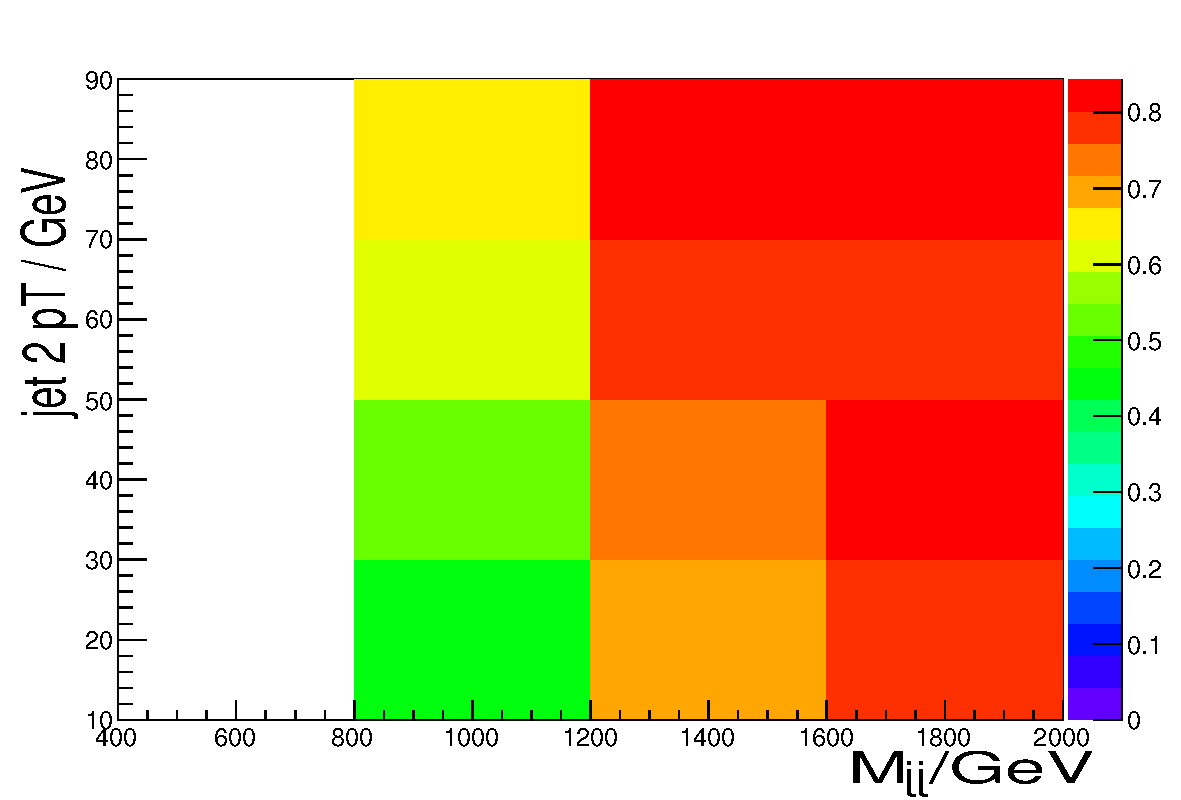
\includegraphics[width=.65\largefigwidth]{plots/parked/HLT_DiJet35_MJJ700_AllJets_DEta3p5_VBFmet120trigeff.pdf}}
  \subfloat[]{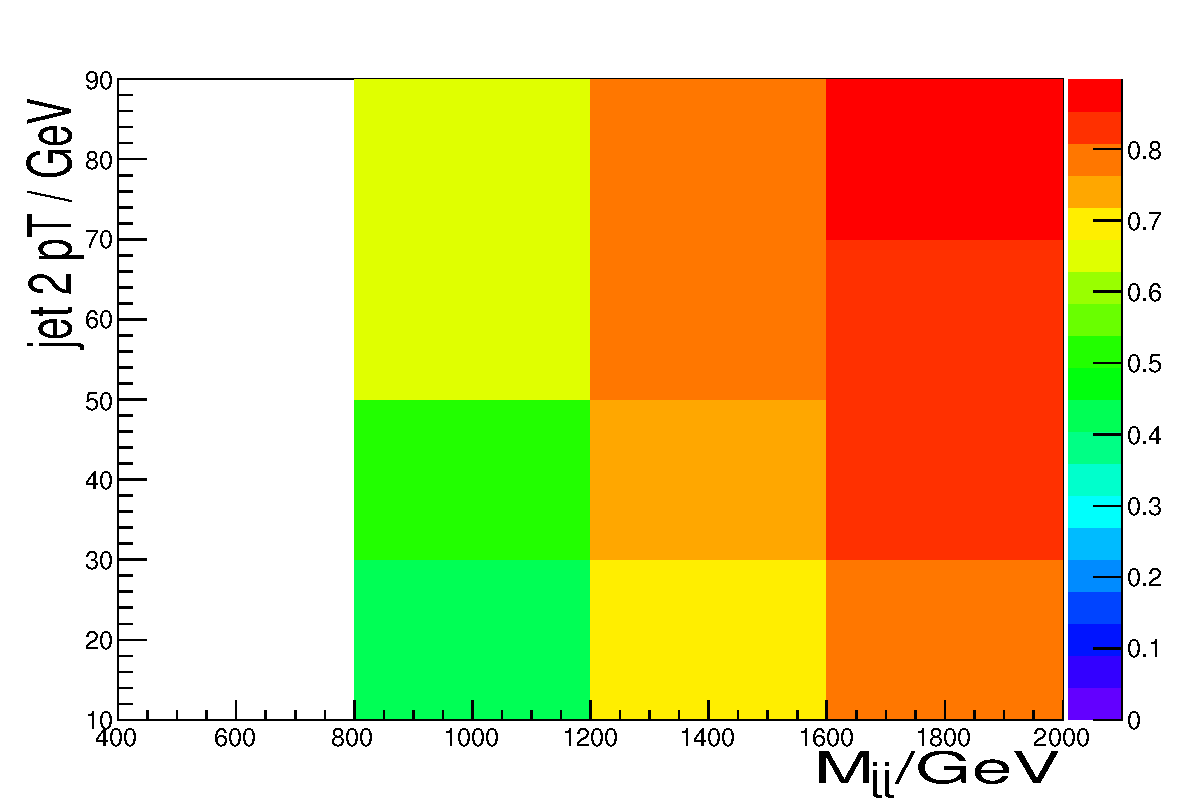
\includegraphics[width=.65\largefigwidth]{plots/parked/HLT_DiJet30_MJJ700_AllJets_DEta3p5_VBFmet120trigeff.pdf}}
 \caption{The efficiency for the trigger (color-scale) used in eras B and C (a) and era D (b), as a function of \Mjj and sub-leading jet \pt for events with \METnoMU between 60 and 120 \GeV. The efficiency was measured using a single muon dataset collected with an orthogonal trigger.}
  \label{fig:parked3dtrigeff}
\end{figure}

In order to achieve a smoother parameterisation of the trigger efficiency, coarse bins in \Mjj and sub-leading jet \pt were chosen, and a fit to the \METnoMU efficiency distribution in each bin was performed, using the following function:
\begin{equation}
  \label{eq:parkedtrigfunc}
  f\left(x\right)=\frac{A}{2}\cdot\left(1+ \frac{2}{\sqrt{\pi}}\int_{0}^{\frac{x-B}{\sqrt{C}}}e^{-t^{2}}\mathrm{d}t\right),
\end{equation}
which has a maximum value of A, and is derived from the error function with centre B and width \DIFaddbegin \DIFadd{related parameter }\DIFaddend C. The width, maximum and centre of the function are all allowed to float in the fit. The events used in this study were required to have leading jet \pt$>50$ \GeV, $\eta_{j1}\cdot\eta_{j2}<0$ and \detajj$>3.6$ to ensure that there are no inefficiencies due to these variables. The results of these fits for the two \Mjj and sub-leading jet \pt bins containing the most events entering the final analysis selection are shown in \FigureRef{fig:parkedtrigeff}. The fit can be seen to describe the data well and the uncertainties are small. The results for the remaining bins are shown in \AppendixRef{app:trigeffs}. Most bins have good agreement between the fit and the data, however, some of the plots in the appendix indicate that the parameters of the fit have taken extreme values, or have very large uncertainties. These extreme values and poor fits are mostly due to low numbers of events in the bin. The analysis selection described in \SectionRef{sec:parkedsel}, ensures that no events in these bins are used in the analysis.

\begin{figure}
  \subfloat[]{\includegraphics[width=.65\largefigwidth]{plots/parked/trigfitplots/hData_MET_1D_35D.pdf}}
  \subfloat[]{\includegraphics[width=.65\largefigwidth]{plots/parked/trigfitplots/hData_MET_1D_45D.pdf}}
  \caption{The results of performing a fit of the function in \EquationRef{eq:parkedtrigfunc} to the efficiency of the trigger used in era D, measured in a sample of single muon events collected with an orthogonal trigger. The dashed bands show the uncertainty on the fit due to each of the three parameters of the fit. The two bins of dijet mass (mjj) and sub-leading jet's \pt (j2pt) shown are those with the two highest numbers of events from the final signal region described in \SectionRef{sec:parkedsel}. The results of the fits in the other bins are shown in \AppendixRef{app:trigeffs}.}
  \label{fig:parkedtrigeff}
\end{figure}

Each \ac{MC} event was weighted by the average of the efficiency found for each of the three triggers weighted by the amount of integrated luminosity recorded using each trigger as shown in the following equation:
\begin{equation}
  \label{eq:parkedtrigweight}
  w\left(p_{\mathrm{T}j2},\Mjj,\METnoMU\right)=\frac{\sum_{i}\mathcal{L}_{i}\epsilon_{i}\left(p_{\mathrm{T}j2},\Mjj,\METnoMU\right)}{\sum_{i}\mathcal{L}_{i}},
\end{equation}
where $i$ are the three triggers, $\epsilon_{i}\left(p_{\mathrm{T}j2},\Mjj,\METnoMU\right)$ is the measured efficiency for trigger $i$ as a function of the event's sub-leading jet \pt, \Mjj and \METnoMU, and $\mathcal{L}_{i}$ is the integrated luminosity collected using trigger $i$. The resulting trigger efficiency varies smoothly and leads to no unphysical discontinuities in the distributions of event variables as can be seen from the figures in the remainder of this chapter.

\section{Event selection}
\label{sec:parkedsel}
As mentioned above\DIFaddbegin \DIFadd{, }\DIFaddend a significant challenge in the analysis of the parked data is that the additional areas of phase space collected by these triggers, but not collected by the prompt data triggers, have very large contributions from \ac{QCD} backgrounds. The \ac{QCD} contribution to \ac{VBF} analyses is very hard to model because \DIFdelbegin \DIFdel{whilst }\DIFdelend \DIFaddbegin \DIFadd{although }\DIFaddend the cross-sections for these processes are very high, the probability of any individual event being \ac{VBF}-like is very low. The number of \ac{MC} events that must be generated to make a representative sample is therefore prohibitively large. As a result of these difficulties, the parked data selection is separated into two stages. The first ``preselection'' stage selects a region of phase space which is not expected to be dominated by \ac{QCD} processes. After this preselection has been made the background processes expected to contribute are the same as in the prompt analysis, and studies were undertaken into which background estimation methods and final signal region selection leads to the best expected limit.

%runcbug101114.pdf sig reg optimisation

\subsection{Preselection}
\label{sec:parkedpresel}
The first element of the preselection was motivated by the trigger. The following selection was applied to ensure that the values of all event variables are above the trigger thresholds of all triggers used, and that the \METnoMU was above the lowest value of the \DIFdelbegin \DIFdel{turn on }\DIFdelend \DIFaddbegin \DIFadd{turn-on }\DIFaddend centre, B, as defined in \EquationRef{eq:parkedtrigfunc}, obtained from the fits described in \SectionRef{sec:parkedtrigger}:
\begin{align}
  \label{eq:parkedprepresel}
  \begin{split}
  \eta_{j1}\cdot\eta_{j2}<0,\,\mathrm{leading\,jet\,}\pt>50 \GeV, \detajj>3.6, \\
  \mathrm{sub-leading\,jet\,}\pt>40 \GeV, \Mjj>800\DIFdelbegin \DIFdel{GeV}\DIFdelend \DIFaddbegin \,\GeV\DIFaddend , \METnoMU>90\GeV.
  \end{split}
\end{align}
Where $j1$ and $j2$ are the leading and sub-leading \pt jets in the event and are chosen as the \ac{VBF} tag jets. We also require that for the ``signal-like'' selection there are no veto electrons or muons in the event. The W+jets and Z+jets control regions used in the background estimates described in \SectionRef{sec:parkedbkg} impose different lepton requirements. QCD multijet processes still dominate the region defined by this selection, as can be seen in \FigureRef{fig:parkedpresel}a, where there are a lot more data events than expected from the background \ac{MC} prediction. This difference is due to mismeasured \ac{QCD} events not being adequately modelled by the available \ac{MC} samples, which are described in further detail in \SectionRef{sec:parkedQCD}. 

Additional selection requirements were applied to reduce the observed differences from the mismeasured \ac{QCD} multijet background. The first variable that was used to achieve this reduction is the \MET significance, \METsig, which is defined as the ratio between \METnoMU and the square root of the sum of the transverse energy of all particles in the event, which is an estimate of the statistical error on the \MET. \DIFaddbegin \DIFadd{As the sum of the square root of the transverse energy of all particles is being used as an estimate of the statistical uncertainty on the }\MET \DIFadd{it has units of }\GeV \DIFadd{and }\METsig \DIFadd{is therefore unitless. }\DIFaddend The intention of the \METsig cut is to remove events which have a large amount of \MET, but also have an even larger amount of visible energy, meaning that the \MET is likely to be from mismeasurement of the visible particles. The preselection requires that \METsig be greater than 3. The value of this cut was chosen by looking at \FigureRef{fig:parkedpresel}a and removing the region with the most disagreement between data and \ac{MC}. \DIFdelbegin \DIFdel{The resulting region}\DIFdelend \DIFaddbegin \DIFadd{While the resulting region, }\DIFaddend shown in \FigureRef{fig:parkedpresel}b\DIFaddbegin \DIFadd{, }\DIFaddend still does not display good data-\ac{MC} agreement, \DIFdelbegin \DIFdel{however }\DIFdelend the disagreement is smaller.

After the cut on \METsig, a requirement that the \METnoMU is not too close to any jets in \phi was made. This requirement was motivated by the fact that if the \MET is due only to the mismeasurement of a jet, the \MET will be aligned with that jet. Two variables were investigated, the first was the minimum azimuthal angle difference between either of the two tag jets and the \METnoMU, \jetmetdphileading, and the second was the minimum azimuthal angle difference between any jet with \pt greater than 30 \GeV and the \METnoMU, \jetmetdphi. At a similar signal efficiency the difference between the observed number of events and the \ac{MC} background prediction, which is an indication of the remaining \ac{QCD} multijet background, was found to be 80\% smaller for a cut on \jetmetdphi than a cut on \jetmetdphileading. The same cut on \jetmetdphi was also found to reduce top quark related backgrounds by a factor of two compared to a cut on \jetmetdphileading. We therefore require that \jetmetdphi$>1.0$ for events to pass the preselection. \jetmetdphi was found to give significantly better signal efficiency than the \dphijj variable used in the prompt analysis for the same background rejection, so no cut was made on \dphijj.

%AN-14-243
\begin{figure}
  \subfloat[]{\includegraphics[width=.7\largefigwidth]{plots/parked/AN-14-243-figs/lognopreselnunu_metnomu_significance.pdf}}
  \subfloat[]{\includegraphics[width=.7\largefigwidth]{plots/parked/AN-14-243-figs/logmetsigpreselnunu_alljetsmetnomu_mindphi.pdf}}

  \subfloat[]{\includegraphics[width=.7\largefigwidth]{plots/parked/AN-14-243-figs/logmjj800nunu_dijet_M.pdf}}
  \caption{(a) \METsig after the \DIFdelbeginFL \DIFdelFL{trigger driven }\DIFdelendFL \DIFaddbeginFL \DIFaddFL{trigger-driven }\DIFaddendFL selection described in \EquationRef{eq:parkedprepresel}. (b) \jetmetdphi after the \DIFdelbeginFL \DIFdelFL{trigger driven }\DIFdelendFL \DIFaddbeginFL \DIFaddFL{trigger-driven }\DIFaddendFL selection and requiring \METsig$>3$. (c) \Mjj after the \DIFdelbeginFL \DIFdelFL{trigger driven }\DIFdelendFL \DIFaddbeginFL \DIFaddFL{trigger-driven }\DIFaddendFL selection and requiring \METsig$>3$ and \jetmetdphi$>1$. All three plots are of the signal-like region with the \ac{MC} scaled using the background estimation methods described in \SectionRef{sec:parkedbkg}. The disagreement between data and the predictions from background \ac{MC} samples is believed to be due to mismeasured \ac{QCD} multijet events which are not well modelled by the available \ac{MC} samples. The last bin of each distribution contains the events above the range displayed. Signal (gg$\rightarrow$H) refers to an \ac{SM} \ac{VBF} (\ac{ggH}) produced Higgs boson with \BRinv=100\%.}
  \label{fig:parkedpresel}
\end{figure}

%contplotsandpresel160914
The \Mjj distribution after the \jetmetdphi cut is shown in \FigureRef{fig:parkedpresel}c. Whilst the agreement for large \Mjj is good, it can be seen that the first bin of the distribution, where mismeasured \ac{QCD} multijet events would be expected, due to \DIFdelbegin \DIFdel{their }\DIFdelend \DIFaddbegin \DIFadd{them }\DIFaddend not recoiling against another object, shows a significant disagreement. The final cut of the preselection is therefore to require \Mjj$>1000$ \GeV. This cut also ensures that none of the bins used to describe the trigger efficiency which have too few events to be reliable are used. In summary the full preselection is as follows:
\begin{equation}
  \label{eq:presel}
  \begin{split}
  \eta_{j1}\cdot\eta_{j2}<0,\,\mathrm{leading\,jet\,}\pt>50 \GeV, \detajj>3.6, \\
  \mathrm{sub-leading\,jet\,}\pt>40 \GeV, \Mjj>1000\DIFdelbegin \DIFdel{GeV}\DIFdelend \DIFaddbegin \,\GeV\DIFaddend , \METnoMU>90\GeV, \\
  \jetmetdphi>1.0, \METsig>3.0.
  \end{split}
\end{equation}
Distributions of several variables after the full preselection are shown in \FigureRef{fig:parkedpostpresel}. No estimate of the \ac{QCD} contribution is given in these distributions, and it can be seen that there is still disagreement between data and \ac{MC} in the areas where \ac{QCD} would be expected to contribute. Further selection is, therefore, necessary.

\begin{figure}
  \includegraphics[width=.65\largefigwidth]{plots/parked/AN-14-243-figs/output_presel/nunu_dijet_deta.pdf}
  \includegraphics[width=.65\largefigwidth]{plots/parked/AN-14-243-figs/output_presel/nunu_dijet_M.pdf}

  \includegraphics[width=.65\largefigwidth]{plots/parked/AN-14-243-figs/output_presel/nunu_jet1_pt.pdf}
  \includegraphics[width=.65\largefigwidth]{plots/parked/AN-14-243-figs/output_presel/nunu_jet2_pt.pdf}

  \includegraphics[width=.65\largefigwidth]{plots/parked/AN-14-243-figs/output_presel/nunu_metnomuons.pdf}
  \includegraphics[width=.65\largefigwidth]{plots/parked/AN-14-243-figs/output_presel/nunu_metnomu_significance.pdf}

  \includegraphics[width=.65\largefigwidth]{plots/parked/AN-14-243-figs/output_presel/nunu_alljetsmetnomu_mindphi.pdf}

  \caption{From top to bottom, left to right, distributions of \detajj, \Mjj, leading jet \pt, sub-leading jet \pt, \METnoMU, \METsig and \jetmetdphi for events passing the full preselection. No \DIFdelbeginFL %DIFDELCMD < \ac{QCD} %%%
\DIFdelendFL \DIFaddbeginFL \DIFaddFL{QCD }\DIFaddendFL contribution is shown, which accounts for the difference between the data observation and background prediction. The last bin of each distribution contains the events above the range displayed.}
  \label{fig:parkedpostpresel}
\end{figure}




\subsection{Signal region selection}
\label{sec:parkedsigsel}
As can be seen from \FigureRef{fig:parkedpostpresel}, there is still a significant difference between the data and the \ac{MC} background prediction. It is also evident that the main areas where disagreement occurs are where contributions from \ac{QCD} backgrounds (which are not included in the figure) would be expected to contribute, at low \METsig and low \jetmetdphi, i.e. with jets close to the \METnoMU. Outside these \ac{QCD}-like regions good agreement between data and \ac{MC} is seen, indicating very low numbers of \ac{QCD} events remaining. The approach taken was to place tight requirements on these two variables to reduce the \ac{QCD} background to be much smaller than the other backgrounds considered. The large uncertainty on any estimate of the number of events from \ac{QCD} multijet processes therefore also \DIFdelbegin \DIFdel{become }\DIFdelend \DIFaddbegin \DIFadd{becomes }\DIFaddend negligible. A requirement that events have $\jetmetdphi>2$ and $\METsig>4$, was therefore imposed. The resulting relatively \ac{QCD}-free ``optimisation'' region was blinded (i.e. the data were not looked at) to use for studies to determine the final signal region selection. All of the studies described in this chapter from this point until the results section were performed blind unless stated otherwise.

Two methods to select the signal region were investigated. The first method was a \DIFdelbegin \DIFdel{cut based }\DIFdelend \DIFaddbegin \DIFadd{cut-based }\DIFaddend selection. Starting from the optimisation region the cuts on \METsig, \jetmetdphi, \detajj, sub-leading jet \pt and \Mjj were varied one at a time and the expected limit for each combination of cuts was calculated. The method described in \SectionRef{sec:stats} was used, with the background estimation techniques and systematic uncertainties described in Sections~\ref{sec:parkedbkg} and \ref{sec:parkedsyst} respectively, to calculate the expected limit. In the case of the \ac{QCD} background, which has only a very small contribution to the signal region, the background estimation was performed once for the optimisation selection and used for all cut values. The estimations for all other background processes were repeated for each set of cuts. After each variable was varied the selection was updated to use the cut value that gave the best expected limit. After all the variables had been varied the process was repeated until no improvement in the expected limit was seen so as to avoid ignoring other better sets of cuts. The cut values that gave the best expected limit define the signal region and are as follows:
\begin{equation}
  \label{eq:parkedsigsel}
  \begin{split}
    \eta_{j1}\cdot\eta_{j2}<0,\detajj>3.6,\,\DIFdelbegin \DIFdel{\mathrm{leading\,jet\,\pt}}\DIFdelend \DIFaddbegin \DIFadd{\mathrm{leading\,jet}}\pt\DIFaddend >50 \GeV,\\
    \DIFdelbegin \DIFdel{\mathrm{sub-leading\,jet\,\pt}}\DIFdelend \DIFaddbegin \DIFadd{\mathrm{sub-leading\,jet}}\pt\DIFaddend >45 \GeV, \Mjj>1200 \GeV,\\
    \METnoMU>90 \GeV, \METsig>4.0,\jetmetdphi>2.3.
  \end{split}
\end{equation}
After this selection was defined \DIFdelbegin \DIFdel{a second }\DIFdelend \DIFaddbegin \DIFadd{an alternative, }\DIFaddend \ac{MVA} based\DIFaddbegin \DIFadd{, }\DIFaddend method of optimising the selection was investigated to see if we could improve on the \DIFdelbegin \DIFdel{cut based }\DIFdelend \DIFaddbegin \DIFadd{cut-based }\DIFaddend selection. \ac{BDT} and \DIFdelbegin \DIFdel{fisher }\DIFdelend \DIFaddbegin \DIFadd{Fisher }\DIFaddend discriminants were trained using signal and background events passing the signal region selection~\cite{TMVA}. The signal region selection was used as the basis for this training so as to ensure that the number of events from the \ac{QCD} background in the studied region was small. The optimisation procedure defined above was then repeated with the value of the discriminant considered as an additional variable. One advantage of \ac{MVA}\DIFdelbegin \DIFdel{based }\DIFdelend \DIFaddbegin \DIFadd{-based }\DIFaddend selection over simple \DIFdelbegin \DIFdel{rectangular cut based }\DIFdelend \DIFaddbegin \DIFadd{cut-based }\DIFaddend selection is that information about the correlation between variables is taken into account. The correlation coefficients between the variables used as inputs to the \ac{MVA} are shown for signal and V+jets background events in \FigureRef{fig:parkedmvacorr}. These variables were chosen as they showed the most difference between signal and background distributions and correlations out of a wide range of variables investigated. Without \DIFdelbegin \DIFdel{the addition of any }\DIFdelend \DIFaddbegin \DIFadd{considering any of the }\DIFaddend additional systematic uncertainties associated with the understanding of the variables input to the \ac{MVA}, the largest improvement in the expected limit was less than 1\%. It was therefore decided to use the \DIFdelbegin \DIFdel{cut based }\DIFdelend \DIFaddbegin \DIFadd{cut-based }\DIFaddend selection as the final event selection.
\begin{figure}
  \subfloat[]{\includegraphics[width=.65\largefigwidth]{plots/parked/AN-14-243-figs/inputcorrsig.pdf}}
  \subfloat[]{\includegraphics[width=.65\largefigwidth]{plots/parked/AN-14-243-figs/inputcorrbkg.pdf}}
  \caption{Matrices of correlation coefficients for several variables in signal (a) and V+jets background (b) events passing the signal region selection. The variables are 1) the azimuthal angle difference between the \METnoMU and the \DIFaddbeginFL \DIFaddFL{vector sum of the }\DIFaddendFL unclustered energy in the event, 2) the square root of the hadronic energy in the event, 3) \METsig, 4) \METnoMU, 5) \Mjj, 6) the number of jets with $\pt>30$ \GeV between the two tag jets in \eta, 7) the vectorial sum of the tag jets \pt and the \METnoMU, 8) the ratio between the magnitude of the vectorial sum of the tag jet's \pt and the \METnoMU.}
  \label{fig:parkedmvacorr}
\end{figure}

\section{Background estimation}                                                                                                                          
\label{sec:parkedbkg}
After the full event selection the V+jets backgrounds, as in the prompt analysis, dominate. Also, as in the prompt analysis, contributions are expected from top quark and diboson related processes. Finally, whilst it is reduced significantly by the selection described above, it is also necessary to estimate the expected contribution from the very small number of remaining \ac{QCD} multijet events.

The methods used to estimate the V+jets backgrounds are based on those used in the prompt analysis. \EquationRef{eq:wdatabkg} is used in several of these methods in this section, and it is repeated here:
\begin{equation}
  \label{eq:wdatabkgrep}
  N^{S}_{Exp}=\left(N^{C}_{Data}-N^{C}_{Bkg}\right)\cdot\frac{N^{S}_{MC}}{N^{C}_{MC}}.
\end{equation}
The terms on the \DIFdelbegin \DIFdel{right hand }\DIFdelend \DIFaddbegin \DIFadd{right-hand }\DIFaddend side of this equation which multiply the estimation from \ac{MC} of the number of events due to a particular background process \DIFaddbegin \DIFadd{in the signal region }\DIFaddend are often collectively referred to as the data-driven scale factor. The changes in event selection for this analysis necessitated several changes from the methods for the prompt analysis. The use of this data-driven method to investigate the top quark related background was also investigated. Furthermore, among other improvements, the systematic uncertainty on the \Znunu background was re-evaluated. All of these changes and improvements are described in this section.

\subsection{Top quarks}
\label{sec:parkedtop}
Almost all top quarks decay to a \PW boson and a b quark. Top quarks are either created in pairs, or via ``single top'' production where only one top quark is created in association with  other quarks or a \PW boson. Top pair production results in two \PW bosons and two b quarks. Single top production results in some combination of \PW bosons and quarks. Either single or pair production of top quarks can result in the appearance of \MET and jets with no leptons, if at least one of the \PW bosons decays leptonically and the lepton is misreconstructed. The resulting jets can coincidentally have \ac{VBF}-like topology. Whilst the contribution from these processes is expected to be small in the signal region, making up around 1\% of events there, the presence of \PW bosons and jets makes these processes very likely to contribute to the control regions used to estimate the $\PW+$jets background contribution. In the $\PW\rightarrow\tau\nu$ control region approximately 15\% of events are estimated to come from top quark processes. \DIFdelbegin \DIFdel{Data driven }\DIFdelend \DIFaddbegin \DIFadd{Data-driven }\DIFaddend methods for estimating the top quark background and its uncertainties were therefore investigated.

Initially, a dilepton control region was investigated. This had the same cuts on the jet and \MET related variables as the signal region, but the lepton veto was replaced with a requirement that there is exactly one tight electron and one tight muon. This final state would be expected in the case of top quark pair production or single top production with a \PW boson, where both the resulting \PW bosons decay leptonically to different flavour leptons. This region had only single figure numbers of events expected, so the cut on \jetmetdphi was loosened to 0. It can be seen from \FigureRef{fig:parkedtopjetmetdphi} that the ratio between data and MC in this region does not depend significantly on \jetmetdphi. The data-driven scale factor obtained from this dilepton region was, within the statistics available, consistent with 1 and a good agreement between data and \ac{MC} was seen in all variables studied. A modification of this control region where events with either two tight electrons or two tight muons, and no other leptons were selected was also studied. This final state would also be expected where two \PW bosons from top quark production decayed leptonically, except this time to the same flavour of lepton. In order to avoid \PZ boson contributions the leptons' invariant mass was required to be incompatible with that of a \PZ boson, i.e. outside of the range from 60 to 120 \GeV. This control region also yielded good data-\ac{MC} agreement and a scale factor compatible with 1. 

\begin{figure}
  \subfloat[]{\includegraphics[width=.65\largefigwidth]{plots/parked/topjetmetdphicut0.pdf}}
  \subfloat[]{\includegraphics[width=.65\largefigwidth]{plots/parked/HIG-14-038-figs/output_sigreg/top_dijet_M.pdf}}
  \caption{The distribution of \jetmetdphi (a) and \Mjj (b) in the top control region with one tight electron and one tight muon. The last bin of each distribution contains the events above the range displayed.}
  \label{fig:parkedtopjetmetdphi}
\end{figure}


An issue with both of these control regions is that the ratio of pair production to single top quark production is very different from both the signal region and the $\PW\rightarrow\tau\nu$ control region. \ac{MC} estimations indicate that these top control regions have a negligible single top contribution, while the top background in the signal region has almost no top quark pair contribution. The $\PW\rightarrow\tau\nu$ region is expected to be a mixture, its top quark background being 30\% from single top events and 70\% for top quark pairs, again estimated from \ac{MC}. A single top control region was therefore also investigated.

The single top region differed from the signal region in that the \jetmetdphi cut was removed, exactly one tight electron or muon was required, further leptons were vetoed and one of the tag jets was required to be compatible with being a b-jet. The restriction to a single lepton significantly reduces the top quark pair production contribution where both resulting \PW bosons decay leptonically, and the requirement of one b-jet reduces the $\PW+$jets contribution. 

Identification of the b-jet was done using the \ac{CSV} discriminant~\cite{bjets}. B quarks are both heavier and longer lived than many other particles created at the \LHC, meaning that their secondary decay vertex can be distinguished from the \ac{PV}. \ac{CSV} is an \ac{MVA} based discriminant which uses information on secondary vertices and the lifetime of the particle to discriminate between jets from b quarks and those from light quarks. The medium working point used for this control region has an efficiency of approximately 85\% for b-quarks and mis-identifies light quark jets as b jets approximately 1\% of the time.

\ac{MC} estimates indicate the single top region is 17\% single top. This region again showed good data-\ac{MC} agreement (as can be seen in \FigureRef{fig:parkedsingletopjetmetdphi}) and a scale factor compatible with 1 within uncertainties. Because good agreement between data and \ac{MC} and scale factors compatible with 1 are seen in all investigated control regions, it was decided to use the \ac{MC} prediction for the top background in all regions with no additional scale factor. A 20\% systematic uncertainty was applied to this prediction which covered the largest deviation from 1 seen in the scale factors from the various control regions.

\begin{figure}
  \subfloat[]{\includegraphics[width=.65\largefigwidth]{plots/parked/output_singletop/top_jetmetnomu_mindphi.pdf}}
  \subfloat[]{\includegraphics[width=.65\largefigwidth]{plots/parked/output_singletop/top_dijet_M.pdf}}
  \caption{The distribution of \jetmetdphileading (a) and \Mjj (b) in the single top control region. The last bin of each distribution contains the events above the range displayed.}
  \label{fig:parkedsingletopjetmetdphi}
\end{figure}

\subsection{W$\rightarrow e\nu$+jets}
\label{sec:parkedwenu}
The $\PW\rightarrow e\nu$ background in the parked data analysis is estimated using the same method as that used for the prompt analysis based on \EquationRef{eq:wdatabkgrep}. The control region used has the same requirements as the signal region, except that the electron veto is replaced with a requirement that there is one tight electron and no other electrons present in the event. The requirement of an electron removes signal events and enriches the region in $\PW\rightarrow e\nu$ events. The distributions of several variables in data and \ac{MC} (which has been scaled by the data-driven scale factor extracted from this control region) are shown in \FigureRef{fig:parkedwenu}, where good agreement can be seen. A table of the inputs to, and results of, \EquationRef{eq:wdatabkgrep} can be seen in \TableRef{tab:parkedwenu}. The table also shows that the expected contribution to this region from other background processes is small, being approximately 5\%. The scale factor obtained for this background is 0.5, which is significantly different from 1, this difference is further investigated in \SectionRef{sec:parkedscalefactors}.

\begin{table}
  \begin{center}
    \caption{The inputs to, and results of, \EquationRef{eq:wdatabkgrep}, when used to estimate the $W\rightarrow e\nu$ estimate in the signal
      region.}
    \label{tab:parkedwenu}
    \begin{tabular}{lcc}
      \hline
      \hline
      & Signal region & Control region \\
      \hline
      \hline
      $N_{Data}$&N/A&$68\pm 8.2$\stat\\
      $N_{Bkg}$&N/A&$3.5\pm 1.2(\rm{MC\,stat})$\\
      $N_{MC}$&$114.9\pm8.9(\rm{MC\,stat})$&$128.0\pm 8.0(\rm{MC\,stat})$\\
      \hline
      \DIFdelbeginFL \DIFdelFL{$\frac{N^{data}-N^{bkg}}{N^{W MC}_{C}}$ }\DIFdelendFL \DIFaddbeginFL \DIFaddFL{$\frac{N^{data}-N^{bkg}}{N^{C}_{MC}}$ }\DIFaddendFL & \multicolumn{2}{c|}{$0.50\pm0.06$\stat$\pm0.03$(MC stat)} \\
      \hline
      $N_{\PW\rightarrow e\nu}$&\textcolor{red}{$57.9\pm7.4$\stat$\pm7.7$\syst}&N/A \\
        \hline
        \hline
    \end{tabular}
  \end{center}
\end{table}

\begin{figure}
  \includegraphics[width=.65\largefigwidth]{plots/parked/HIG-14-038-figs/output_sigreg/enu_dijet_deta.pdf}
  \includegraphics[width=.65\largefigwidth]{plots/parked/HIG-14-038-figs/output_sigreg/enu_dijet_M.pdf}

  \includegraphics[width=.65\largefigwidth]{plots/parked/HIG-14-038-figs/output_sigreg/enu_jet1_pt.pdf}
  \includegraphics[width=.65\largefigwidth]{plots/parked/HIG-14-038-figs/output_sigreg/enu_jet2_pt.pdf}

  \includegraphics[width=.65\largefigwidth]{plots/parked/HIG-14-038-figs/output_sigreg/enu_metnomuons.pdf}
  \includegraphics[width=.65\largefigwidth]{plots/parked/HIG-14-038-figs/output_sigreg/enu_metnomu_significance.pdf}

  \includegraphics[width=.65\largefigwidth]{plots/parked/HIG-14-038-figs/output_sigreg/enu_alljetsmetnomu_mindphi.pdf}

  \DIFdelbeginFL %DIFDELCMD < \caption{%%%
\DIFdelendFL \DIFaddbeginFL \caption[Distributions of variables in data and \ac{MC} in the $\PW\rightarrow e\nu$ control region. \ac{MC} events from V+jets backgrounds are scaled by their data-driven scale factors. The variables shown are from top to bottom and left to right: \detajj, \Mjj, the leading and sub-leading jet's \pt, \METnoMU, \METsig and \jetmetdphi. The last bin of each distribution contains the events above the range displayed.]{\DIFaddendFL Distributions of variables in data and \ac{MC} \DIFdelbeginFL \DIFdelFL{events }\DIFdelendFL in the $\PW\rightarrow e\nu$ control region. \ac{MC} events from V+jets backgrounds are scaled by their data-driven scale factors. The variables shown are from top to bottom and left to right\DIFaddbeginFL \DIFaddFL{: }\DIFaddendFL \detajj, \Mjj, the leading and sub-leading jet's \pt, \METnoMU, \METsig and \jetmetdphi. The last bin of each distribution contains the events above the range displayed~\cite{CMS-PAS-HIG-14-038}.}
  \label{fig:parkedwenu}
\end{figure}

\subsection{W$\rightarrow \mu\nu$+jets}
\label{sec:parkedwmunu}
As for the $\PW\rightarrow e\nu$ background the $W\rightarrow \mu\nu$ background is estimated using \EquationRef{eq:wdatabkgrep} with a control region enriched in $\PW\rightarrow\mu\nu$ events through a change in lepton requirements. The control region used has the same requirements as the signal region, but with the muon veto replaced with a requirement that there is one tight muon and no other muons present in the event. The distributions of several variables in data and \ac{MC} (which has been scaled by the data-driven scale factor extracted from this control region) are shown in \FigureRef{fig:parkedwmunu}, where good agreement can be seen. A table of the inputs to, and results of, \EquationRef{eq:wdatabkgrep} can be seen in \TableRef{tab:parkedwmunu}. The contribution from other backgrounds in the $\PW\rightarrow\mu\nu$ control region is approximately 5\%. Again the scale factor obtained  for this background is significantly different from 1, being 0.71, and further investigation of this is detailed in \SectionRef{sec:parkedscalefactors}. Furthermore, the estimated contribution from this background is very different to that expected from $\PW\rightarrow e\nu$, an investigation of this difference is described in \SectionRef{sec:parkedenumunudiff}.

\begin{figure}
  \includegraphics[width=.65\largefigwidth]{plots/parked/HIG-14-038-figs/output_sigreg/munu_dijet_deta.pdf}
  \includegraphics[width=.65\largefigwidth]{plots/parked/HIG-14-038-figs/output_sigreg/munu_dijet_M.pdf}

  \includegraphics[width=.65\largefigwidth]{plots/parked/HIG-14-038-figs/output_sigreg/munu_jet1_pt.pdf}
  \includegraphics[width=.65\largefigwidth]{plots/parked/HIG-14-038-figs/output_sigreg/munu_jet2_pt.pdf}

  \includegraphics[width=.65\largefigwidth]{plots/parked/HIG-14-038-figs/output_sigreg/munu_metnomuons.pdf}
  \includegraphics[width=.65\largefigwidth]{plots/parked/HIG-14-038-figs/output_sigreg/munu_metnomu_significance.pdf}

  \includegraphics[width=.65\largefigwidth]{plots/parked/HIG-14-038-figs/output_sigreg/munu_alljetsmetnomu_mindphi.pdf}
    \DIFdelbeginFL %DIFDELCMD < \caption{%%%
\DIFdelendFL \DIFaddbeginFL \caption[Distributions of variables in data and MC in the $\PW\rightarrow \mu\nu$ control region. MC events from V+jets backgrounds are scaled by their data-driven scale factors. The variables shown are from top to bottom and left to right: \detajj, \Mjj, the leading and sub-leading jet's \pt, \METnoMU, \METsig and \jetmetdphi. The last bin of each distribution contains the events above the range displayed.]{\DIFaddendFL Distributions of variables in data and \DIFdelbeginFL %DIFDELCMD < \ac{MC} %%%
\DIFdelFL{events }\DIFdelendFL \DIFaddbeginFL \DIFaddFL{MC }\DIFaddendFL in the $\PW\rightarrow \mu\nu$ control region. \DIFdelbeginFL %DIFDELCMD < \ac{MC} %%%
\DIFdelendFL \DIFaddbeginFL \DIFaddFL{MC }\DIFaddendFL events from V+jets backgrounds are scaled by their data-driven scale factors. The variables shown are from top to bottom and left to right\DIFaddbeginFL \DIFaddFL{: }\DIFaddendFL \detajj, \Mjj, the leading and sub-leading jet's \pt, \METnoMU, \METsig and \jetmetdphi. The last bin of each distribution contains the events above the range displayed~\cite{CMS-PAS-HIG-14-038}.}
  \label{fig:parkedwmunu}
\end{figure}

\begin{table}[h!]
  \begin{center}
    \caption{The inputs to, and results of, \EquationRef{eq:wdatabkgrep}, when used to estimate the $W\rightarrow \mu\nu$ estimate in the signal
      region.}
    \label{tab:parkedwmunu}
    \begin{tabular}{lcc}
      \hline
      \hline
      & Signal region & Control region \\
      \hline
      \hline
      $N_{Data}$&N/A&$300\pm 17.3$\stat\\
      $N_{Bkg}$&N/A&$14.8\pm 2.5(\rm{MC\,stat})$\\
      $N_{MC}$&$143.7\pm10.2(\rm{MC\,stat})$&$399.9\pm 14.9(\rm{MC\,stat})$\\
      \hline
      \DIFdelbeginFL \DIFdelFL{$\frac{N^{data}-N^{bkg}}{N^{MC}_{C}}$ }\DIFdelendFL \DIFaddbeginFL \DIFaddFL{$\frac{N^{data}-N^{bkg}}{N^{C}_{MC}}$ }\DIFaddendFL & \multicolumn{2}{c|}{$0.71\pm0.04$\stat$\pm0.03$(MC stat)} \\
      \hline
      $N_{\PW\rightarrow\mu\nu}$&\textcolor{red}{$102.5\pm6.2$\stat$\pm11.7$\syst}&N/A \\
      \hline
      \hline
    \end{tabular}
  \end{center}
\end{table}



\subsection{W$\rightarrow \tau\nu$+jets}
\label{sec:parkedwtaunu}
The signal region requirements do not include a veto of hadronic taus, due to the low identification efficiency and relatively high probability for a jet to be identified as a fake tau. Requiring that there is an identified hadronic tau in addition to the signal region selection results in a region containing only 2 data events. In order to increase the number of events in the tau control region the \jetmetdphi cut was removed. The requirement that there is an identified tau reduces the \ac{QCD} multijet contribution in the low \jetmetdphi region significantly compared to what was seen during the choice of the preselection. However, poor data-\ac{MC} agreement was still observed in the \jetmetdphi$<1$ region, which is evidence that some events from multijet processes are still present. To remove these \ac{QCD} multijet events, whilst keeping a reasonable number of events in the resulting control region, a requirement that \jetmetdphileading is greater than 1 and that the transverse mass of the hadronic tau and \MET system is greater than 20 \GeV is applied. The \jetmetdphileading requirement reduces \ac{QCD} backgrounds for the same reason that \jetmetdphi does, but it is a slightly looser requirement as it only considers the two leading jets. The transverse mass of the tau-\MET system is a good variable to reject \ac{QCD} where a lepton is present as in real \PW boson events the tau and \MET are expected to originate from the same object and therefore have significant invariant mass, which is not the case for \ac{QCD} multijet events.

After the anti-\ac{QCD} cuts the agreement between data and \ac{MC} is good as can be seen in \FigureRef{fig:parkedwtaunu}. To account for the different \jetmetdphi selection in this region and the signal region, the data-driven scale factor was calculated both in the $\PW\rightarrow\mu\nu$ control region, which has the signal region \jetmetdphi selection, and in a modified single muon control region with the $\PW\rightarrow\tau\nu$ control region \jetmetdphi selection. The difference between these two scale factors was found to be 20\%, so a 20\% systematic uncertainty was added to the estimate of the $\PW\rightarrow\tau\nu$ background.

The single tau control region with a \jetmetdphileading cut and no \jetmetdphi cut was used with \EquationRef{eq:wdatabkgrep} to estimate the number of $\PW\rightarrow\tau\nu$ events in the signal region. A table of the inputs to, and results of, \EquationRef{eq:wdatabkgrep} can be seen in \TableRef{tab:parkedwtaunu}. The contribution from other backgrounds in the $\PW\rightarrow\tau\nu$ control region is approximately 15\%, with most of these other background events being due to top quark related processes. The scale factor obtained for this background is 0.78, which is closer to 1 than those seen in the other $\PW+$jets backgrounds, however it also has the largest uncertainty. Further investigation of the V+jets scale factors is detailed in \SectionRef{sec:parkedscalefactors}.

\begin{figure}
  \includegraphics[width=.65\largefigwidth]{plots/parked/HIG-14-038-figs/output_sigreg/taunu_dijet_deta.pdf}
  \includegraphics[width=.65\largefigwidth]{plots/parked/HIG-14-038-figs/output_sigreg/taunu_dijet_M.pdf}

  \includegraphics[width=.65\largefigwidth]{plots/parked/HIG-14-038-figs/output_sigreg/taunu_jet1_pt.pdf}
  \includegraphics[width=.65\largefigwidth]{plots/parked/HIG-14-038-figs/output_sigreg/taunu_jet2_pt.pdf}

  \includegraphics[width=.65\largefigwidth]{plots/parked/HIG-14-038-figs/output_sigreg/taunu_metnomuons.pdf}
  \includegraphics[width=.65\largefigwidth]{plots/parked/HIG-14-038-figs/output_sigreg/taunu_metnomu_significance.pdf}

  \includegraphics[width=.65\largefigwidth]{plots/parked/HIG-14-038-figs/output_sigreg/taunu_jetmetnomu_mindphi.pdf}
  \includegraphics[width=.65\largefigwidth]{plots/parked/HIG-14-038-figs/output_sigreg/taunu_lep_mt.pdf}
  \DIFdelbeginFL %DIFDELCMD < \caption{%%%
\DIFdelendFL \DIFaddbeginFL \caption[Distributions of variables in data and MC in the $\PW\rightarrow \tau\nu$ control region. MC events from V+jets backgrounds are scaled by their data-driven scale factors. The variables shown are from top to bottom and left to right: \detajj, \Mjj, the leading and sub-leading jet's \pt, \METnoMU, \METsig, \jetmetdphileading and the tau-\MET system's transverse mass. The last bin of each distribution contains the events above the range displayed.]{\DIFaddendFL Distributions of variables in data and \DIFdelbeginFL %DIFDELCMD < \ac{MC} %%%
\DIFdelFL{events }\DIFdelendFL \DIFaddbeginFL \DIFaddFL{MC }\DIFaddendFL in the \DIFdelbeginFL \DIFdelFL{$\PW\rightarrow e\nu$ }\DIFdelendFL \DIFaddbeginFL \DIFaddFL{$\PW\rightarrow \tau\nu$ }\DIFaddendFL control region. \DIFdelbeginFL %DIFDELCMD < \ac{MC} %%%
\DIFdelendFL \DIFaddbeginFL \DIFaddFL{MC }\DIFaddendFL events from V+jets backgrounds are scaled by their data-driven scale factors. The variables shown are from top to bottom and left to right\DIFaddbeginFL \DIFaddFL{: }\DIFaddendFL \detajj, \Mjj, the leading and sub-leading jet's \pt, \METnoMU, \METsig, \jetmetdphileading and the tau-\MET system's transverse mass. The last bin of each distribution contains the events above the range displayed~\cite{CMS-PAS-HIG-14-038}.}
  \label{fig:parkedwtaunu}
\end{figure}

\begin{table}[h!]
  \begin{center}
    \caption{The inputs to, and results of, \EquationRef{eq:wdatabkgrep}, when used to estimate the $W\rightarrow \tau\nu$ estimate in the signal
      region.}
    \label{tab:parkedwtaunu}
    \begin{tabular}{lcc}
      \hline
      \hline
      & Signal region & Control region \\
      \hline
      \hline
      $N_{Data}$&N/A&$76\pm 8.7$\stat\\
      $N_{Bkg}$&N/A&$13.3\pm 2.8(\rm{MC\,stat})$\\
      $N_{MC}$&$121.9\pm 8.7(\rm{MC\,stat})$&$80.8\pm 6.4(\rm{MC\,stat})$\\
      \hline
      \DIFdelbeginFL \DIFdelFL{$\frac{N^{data}-N^{bkg}}{N^{MC}_{C}}$ }\DIFdelendFL \DIFaddbeginFL \DIFaddFL{$\frac{N^{data}-N^{bkg}}{N^{C}_{MC}}$ }\DIFaddendFL & \multicolumn{2}{c|}{$0.78\pm 0.11$\stat$\pm 0.07$(MC stat)} \\
      \hline
      $N_{\PW\rightarrow\mu\nu}$&\textcolor{red}{$94.6\pm 13.1$\stat$\pm 23.8$\syst}&N/A \\
      \hline
      \hline
    \end{tabular}
  \end{center}
\end{table}



\subsection{Differences between the $W\rightarrow e\nu$, $W\rightarrow\mu\nu$ and $W\rightarrow\tau\nu$ +jets backgrounds}
\label{sec:parkedenumunudiff}
%tau easily explainable by id eff
%sf for enu and munu different but compatible MC yield is where main difference is separate into into and out of acceptance and why (electrons in HF are jets, electron ID eff slightly worse) mindphijetmet shape difference outside acceptance
The number of W+jets events decaying to a particular flavour of lepton with \ac{VBF}-like jet kinematics should be the same for all three flavours of lepton through lepton universality. Differences between the numbers of background events from $\PW\rightarrow e\nu$, $\PW\rightarrow \mu\nu$ and $\PW\rightarrow \tau\nu$ must therefore be due to differences in the identification of the leptons. Hadronic taus have much lower identification efficiencies than the other two flavours of leptons, so might naively be expected to give rise to a much larger number of background events. However, due to the similarities between hadronic taus and jets, unidentified taus often lead to additional jets in the event and therefore increase the probability that an event will fail the \jetmetdphi cut~\cite{CMS-PAS-TAU-11-001}. These two competing effects mean that the number of background events from $\PW\rightarrow\tau\nu$ passing the signal region selection is not necessarily expected to be the same as that from $\PW\rightarrow e\nu$ and $\PW\rightarrow\mu\nu$.

\DIFdelbegin \DIFdel{By contrast, electrons and muons have much more similar }\DIFdelend %DIF > ??proof read this section
\DIFaddbegin \DIFadd{Electrons and muons also have different }\DIFaddend identification efficiencies (see Sections~\ref{sec:electrons} and \ref{sec:muons})\DIFdelbegin \DIFdel{. The }\DIFdelend \DIFaddbegin \DIFadd{, so they are not expected to lead to identical numbers of events. However, the }\DIFaddend 45\% difference seen in the number of expected background events from these two processes  was \DIFdelbegin \DIFdel{therefore unexpected. This difference was also not }\DIFdelend \DIFaddbegin \DIFadd{larger than that }\DIFaddend seen in the prompt analysis, as can be seen from \TableRef{tab:promptresults}. The prediction of the $\PW\rightarrow e/\mu\nu$ backgrounds is made up of a data-driven scale factor and an estimate from \ac{MC} of the number of events from the process expected in the signal region, $N_{MC}^{S}$. Both these elements were studied to try to understand \DIFaddbegin \DIFadd{whether }\DIFaddend the observed differences \DIFaddbegin \DIFadd{can be explained by the different identification efficiencies or if another effect is responsible}\DIFaddend .

Firstly, the data-driven scale factors for the electron and muon backgrounds differ by 30\%, which is not sufficient to explain the full difference between the electron and muon background estimates. Furthermore, when systematic errors are taken into account this difference is only approximately one standard deviation. On the other hand, $N_{MC}^{S}$ does show a significant difference.

To study the difference in $N_{MC}^{S}$ two sub-regions of the signal region were studied, that with a generator-level lepton inside the detector acceptance for both electrons and muons (\DIFdelbegin \DIFdel{$|\eta<2.1$}\DIFdelend \DIFaddbegin \DIFadd{$|\eta|<2.1$}\DIFaddend ), and that with a generator lepton outside the detector acceptance for both electrons and muons ($|\eta|>2.4$). The number of events in these two sub-regions from both $\PW\rightarrow e\nu$ and $\PW\rightarrow\mu\nu$ \ac{MC} can be seen in \TableRef{tab:enumunudiff}. The numbers of events with a generator level lepton inside acceptance are approximately one standard deviation higher for electrons. This small difference is expected due to the lower identification efficiency for veto \DIFdelbegin \DIFdel{leptons }\DIFdelend \DIFaddbegin \DIFadd{electrons }\DIFaddend making them less likely to cause an event to fail the lepton veto. Distributions of several variables were also studied for events inside the acceptance and found to be very similar for both $\PW\rightarrow e\nu$ and $\PW\rightarrow\mu\nu$ events.

Outside the acceptance there are a lot more muon events than electron events. In this region neither flavour of lepton can be reconstructed and therefore cannot lead to an event failing the lepton veto, which implies that any difference is due to one or both flavours of lepton being reconstructed as a different object and affecting the jet or \MET related variables in the signal region selection. To study this effect further, the \jetmetdphi requirement was relaxed to 1 and the distributions of several variables plotted for electron and muon events outside the acceptance. Three of these distributions are shown in \FigureRef{fig:enumunudiff}. It can be seen from \FigureRef{fig:enumunudiff}a that electron events generally have more jets than muon events. \FigureRef{fig:enumunudiff}b indicates that the electron events also have much lower values of \jetmetdphi. Finally, \FigureRef{fig:enumunudiff}c shows that there are very few events passing this region's selection requirements which have a generator-level electron with \pt$>30$ \GeV, the threshold for jets to be included in the \jetmetdphi cut. These three pieces of information suggest that electrons are being reconstructed as jets when outside acceptance significantly more often than muons are. These misreconstructed jets then cause the electron events to fail the \jetmetdphi requirement.

It is to be expected that electrons outside of the detector acceptance will be reconstructed as jets, as these electrons will only be seen as deposits in the forward \ac{HCAL} and therefore be indistinguishable from jets. By contrast, muons deposit very little energy in the calorimeter systems, so will simply not be identified if they are outside the acceptance of the muon system. In the prompt analysis, no requirements were made on jets which were further forward in $\eta$ than the tag jets, explaining why the difference in the numbers of $\PW\rightarrow e\nu$ and $\PW\rightarrow\mu\nu$ events was \DIFdelbegin \DIFdel{not seen }\DIFdelend \DIFaddbegin \DIFadd{much smaller }\DIFaddend there.

\begin{table}
  \caption{The numbers of events predicted by \ac{MC} in the two sub-regions of the signal region with a generator-level lepton that is inside/outside the detector acceptance for both electrons and muons from $\PW\rightarrow e\nu$ and $\PW\rightarrow\mu\nu$ processes. The errors shown are the \ac{MC} statistical uncertainties.}
  \label{tab:enumunudiff}
  \begin{tabular}{lcc}
    \hline
    \hline
    Process & Inside acceptance & Outside acceptance \\
    \hline
    $\PW\rightarrow e\nu$ & $73.7\pm 6.8$ & $30.2\pm 4.9$ \\
    $\PW\rightarrow \mu\nu$ & $61.5\pm 6.8$ & $74.4\pm7.3$ \\
    \hline
    \hline
  \end{tabular}
\end{table}

\begin{figure}
  \subfloat[]{\includegraphics[width=.65\largefigwidth]{plots/parked/AN-14-243-figs/genlepstudy/outsideaccloosedphi/nunu_n_jets_15.pdf}}
  \subfloat[]{\includegraphics[width=.65\largefigwidth]{plots/parked/AN-14-243-figs/genlepstudy/outsideaccloosedphi/nunu_alljetsmetnomu_mindphi.pdf}}

  \subfloat[]{\includegraphics[width=.65\largefigwidth]{plots/parked/AN-14-243-figs/genlepstudy/outsideaccloosedphi/nunu_genlep1_pt.pdf}}
  \caption{Distributions of the number of jets with \pt$>15$ \GeV (a), \jetmetdphi (b) and the \pt of the leading generator-level electron/muon (c) in $\PW\rightarrow e/\mu\nu$ events in a region with cuts which are the same as those of the signal region except that the \jetmetdphi requirement has been loosened to 1 and a generator level lepton outside the detector acceptance for both electrons and muons is required. The last bin of each distribution contains the events above the range displayed.}
  \label{fig:enumunudiff}
\end{figure}

\subsection{Z$\rightarrow \nu\nu$+jets}
\label{sec:parkedznunu}
%same as before studies of uncertainty with madgraph and mcfm
The irreducible $\PZ\rightarrow\nu\nu$ background is estimated using a very similar method to that used in the prompt analysis (\SectionRef{sec:promptznunu}). A reminder of the method highlighting the differences from the prompt analysis is given here.

The method starts by defining a dimuon control region by taking the signal region requirements and replacing the muon veto with the requirement that there are two tight muons with invariant mass compatible with a \PZ boson, i.e. between 60 and 120 \GeV, and no other muons in the event. The number of events in this dimuon control region is then extrapolated to the signal region using efficiencies and cross-section ratios calculated using \ac{MC} events. As in the prompt analysis\DIFaddbegin \DIFadd{, }\DIFaddend a \Zmumu \ac{MC} sample with the reconstructed leptons ignored and a requirement that there is a generator-level dimuon system with invariant mass between 80 and 100 \GeV (i.e. compatible with a \PZ boson) is used to estimate the contribution in the signal region from \Znunu processes. The mass window used here is tighter than that used to define the dimuon control region because the generator level lepton \pt resolution is better than that of reconstructed leptons. \Znunu \ac{MC} events are not used for this estimation due to the limited size of the available \Znunu \ac{MC} samples. Whilst the number of events in the dimuon control region is small the agreement between data and \ac{MC} is good as can be seen from \FigureRef{fig:parkedznunu}\DIFaddbegin \DIFadd{.
}\DIFaddend 

\begin{figure}
  \includegraphics[width=.65\largefigwidth]{plots/parked/HIG-14-038-figs/output_sigreg/mumu_dijet_deta.pdf}
  \includegraphics[width=.65\largefigwidth]{plots/parked/HIG-14-038-figs/output_sigreg/mumu_dijet_M.pdf}

  \includegraphics[width=.65\largefigwidth]{plots/parked/HIG-14-038-figs/output_sigreg/mumu_jet1_pt.pdf}
  \includegraphics[width=.65\largefigwidth]{plots/parked/HIG-14-038-figs/output_sigreg/mumu_jet2_pt.pdf}

  \includegraphics[width=.65\largefigwidth]{plots/parked/HIG-14-038-figs/output_sigreg/mumu_metnomuons.pdf}
  \includegraphics[width=.65\largefigwidth]{plots/parked/HIG-14-038-figs/output_sigreg/mumu_metnomu_significance.pdf}

  \includegraphics[width=.65\largefigwidth]{plots/parked/HIG-14-038-figs/output_sigreg/mumu_jetmetnomu_mindphi.pdf}
  \includegraphics[width=.65\largefigwidth]{plots/parked/HIG-14-038-figs/output_sigreg/mumu_m_mumu.pdf}
  \DIFdelbeginFL %DIFDELCMD < \caption{%%%
\DIFdelendFL \DIFaddbeginFL \caption[Distributions of variables in data and MC in the dimuon control region. MC events from V+jets backgrounds are scaled by their data-driven scale factors. The variables shown are from top to bottom and left to right: \detajj, \Mjj, the leading and sub-leading jet's \pt, \METnoMU, \METsig, \jetmetdphileading and the invariant mass of the dimuon system. The contributions to this region from electroweak and QCD produced $\PZ+$jets events are shown separately. The last bin of each distribution contains the events above the range displayed.]{\DIFaddendFL Distributions of variables in data and \DIFdelbeginFL %DIFDELCMD < \ac{MC} %%%
\DIFdelFL{events }\DIFdelendFL \DIFaddbeginFL \DIFaddFL{MC }\DIFaddendFL in the dimuon control region. \DIFdelbeginFL %DIFDELCMD < \ac{MC} %%%
\DIFdelendFL \DIFaddbeginFL \DIFaddFL{MC }\DIFaddendFL events from V+jets backgrounds are scaled by their data-driven scale factors. The variables shown are from top to bottom and left to right\DIFaddbeginFL \DIFaddFL{: }\DIFaddendFL \detajj, \Mjj, the leading and sub-leading jet's \pt, \METnoMU, \METsig, \jetmetdphileading and the invariant mass of the dimuon system. The contributions to this region from electroweak and \DIFdelbeginFL %DIFDELCMD < \ac{QCD} %%%
\DIFdelendFL \DIFaddbeginFL \DIFaddFL{QCD }\DIFaddendFL produced $\PZ+$jets events are shown separately. The last bin of each distribution contains the events above the range displayed~\cite{CMS-PAS-HIG-14-038}.}
  \label{fig:parkedznunu}
\end{figure}

The formulae used to carry out the extrapolation from the control region to the signal region are given in Equation~\ref{eq:zdatabkg} which is repeated here for reference:
\begin{equation}
  \label{eq:zdatabkgrep}
  N^{S}_{Exp}=\left(N^{C}_{Data}-N^{C}_{Bkg}\right)\cdot\frac{\sigma\left(\PZ\rightarrow\nu\nu\right)}{\sigma\left(\PZ/\gamma^{*}\rightarrow\mu\mu\right)}\cdot\DIFdelbegin \DIFdel{\frac{\epsilon^{S}_{VBF}}{\epsilon^{C}_{VBF}}}\DIFdelend \DIFaddbegin \DIFadd{\frac{\epsilon^{S}_{\mbox{mathrm{VBF}}}}{\epsilon^{C}_{\mbox{VBF}}}}\DIFaddend ,
\end{equation}
where $\epsilon^{S}$ and $\epsilon^{C}$ are calculated as in Equations~\ref{eq:zdataeffs} and \ref{eq:zdataeffc} repeated here:
\begin{align}
  \label{eq:zdataeffsrep}
  \epsilon^{S}\DIFdelbegin \DIFdel{_{VBF}}\DIFdelend \DIFaddbegin \DIFadd{_{\mbox{VBF}}}\DIFaddend &=\frac{ \sigma\left(\PZ\rightarrow\nu\nu,EWK\right) \frac{N^{S}_{MC}\left(EWK\right)} {N_{gen}\left(\PZ \rm{mass},EWK\right)} + \sigma\left(\PZ\rightarrow\nu\nu,QCD\right) \frac{N^{S}_{MC}\left(QCD\right)} {N_{gen}\left(\PZ \rm{mass},QCD\right)} } {\sigma\left(\PZ\rightarrow\nu\nu,EWK\right) + \sigma\left(\PZ\rightarrow\nu\nu,QCD\right)},\\
  \label{eq:zdataeffcrep}
  \epsilon^{C}\DIFdelbegin \DIFdel{_{VBF}}\DIFdelend \DIFaddbegin \DIFadd{_{\mbox{VBF}}}\DIFaddend &=\DIFdelbegin \DIFdel{\frac{  \sigma\left(\PZ/\gamma^{*}\rightarrow\mu\mu,EWK\right) \frac{N^{C}_{MC}\left(EWK\right)} {N_{gen}\left(EWK\right)} + \sigma\left(\PZ/\gamma^{*}\rightarrow\mu\mu,QCD\right) \frac{N^{S}_{MC}\left(QCD\right)} {N_{gen}\left(QCD\right)}  }{\sigma\left(\PZ/\gamma^{*}\rightarrow\mu\mu,EWK\right)+\sigma\left(\PZ/\gamma^{*}\rightarrow\mu\mu,QCD\right)}}\DIFdelend \DIFaddbegin \DIFadd{\frac{  \sigma\left(\PZ/\gamma^{*}\rightarrow\mu\mu,EWK\right) \frac{N^{C}_{MC}\left(EWK\right)} {N_{gen}\left(EWK\right)} + \sigma\left(\PZ/\gamma^{*}\rightarrow\mu\mu,QCD\right) \frac{N^{C}_{MC}\left(QCD\right)} {N_{gen}\left(QCD\right)}  }{\sigma\left(\PZ/\gamma^{*}\rightarrow\mu\mu,EWK\right)+\sigma\left(\PZ/\gamma^{*}\rightarrow\mu\mu,QCD\right)}}\DIFaddend .
\end{align}
As the \Zmumu and \Znunu cross-sections are calculated before the analysis selection cuts and do not depend on detector calibration, the same values are used as in the prompt analysis shown in \TableRef{tab:promptznunueffs}. The other inputs to the above equations and the results of the estimation are shown in \TableRef{tab:parkedznunu}.

Although it is not used in the \Znunu background estimation method, the ratio between the number of \ac{MC} dimuon events, both from electroweak and \ac{QCD} events, and the number of data events minus expected backgrounds from other processes is shown for comparison with the data-driven scale factors used in the $\PW+$jets background estimate. The ratio is, like those in the $\PW+$jets background estimation found to be significantly different from 1. 
%inputs where the same and where different from prompt

\begin{table}
  \caption{The inputs to Equations~\ref{eq:zdatabkgrep}, ~\ref{eq:zdataeffsrep} and ~\ref{eq:zdataeffcrep} and the final estimate of the \Znunu background in the signal region for the parked data analysis. Also shown for comparison is the ratio between the \DIFdelbeginFL %DIFDELCMD < \ac{MC} %%%
\DIFdelendFL \DIFaddbeginFL \DIFaddFL{MC }\DIFaddendFL prediction of the number of \Zmumu events in the control region and the number of data events in the control region. The systematic uncertainties quoted include MC statistical uncertainties and all sources listed in \SectionRef{sec:parkedsyst}. }
  \label{tab:parkedznunu}
  \begin{tabular}{lcc}
    \hline
    \hline
    $N_{gen}\left(\mathnormal{EWK}\right)$&\multicolumn{2}{c}{5781.9}\\
    $N_{gen}\left(\PZ\rm{mass},\mathnormal{EWK}\right)$&\multicolumn{2}{c}{4226.5}\\
    $N_{gen}\left(\mathnormal{QCD}\right)$&\multicolumn{2}{c}{22789000}\\
    $N_{gen}\left(\PZ\rm{mass},\mathnormal{QCD}\right)$&\multicolumn{2}{c}{20334000}\\
    \hline
    \hline
    & Signal region & Control region \\
    \hline
    \hline
    $N_{Data}$ & N/A & $18\pm 4.2\stat$ \\
    $N_{Bkg}$ & N/A & $0.2\pm 0.1 (\rm{MC\,stat})$ \\
    $N_{MC}\left(EWK\right)$ & $7.9\pm 0.2 (\rm{MC\,stat})$& $6.0\pm 0.2 (\rm{MC\,stat})$ \\
    $N_{MC}\left(QCD\right)$ & $29.5\pm 3.0 (\rm{MC\,stat})$ & $20.5\pm 2.5 (\rm{MC\,stat})$ \\
    \hline
    $\frac{N^{C}_{Data}-N^{C}_{Bkg}}{N^{C}_{MC}\left(EWK\right)+N^{C}_{MC}\left(QCD\right)}$ & \multicolumn{2}{c}{$0.67\pm 0.16\stat\pm 0.06 (\rm{MC\,stat})$} \\
    \hline
    $N_{\PZ\rightarrow \nu\nu/\PZ\rightarrow/\gamma^{*}\rightarrow\mu\mu}$ & $\textcolor{red}{158.1\pm 37.8\stat\pm 21.2\syst}$ & $17.8\pm 4.2\stat\pm 0.1 (\rm{MC\,stat})$ \\
    \hline
    \hline
  \end{tabular}
\end{table}

%studies of uncertainty on cross-section ratio
In the prompt analysis one of the largest uncertainties, being 44\% of the size of the total systematic uncertainty on the total background estimate, was the uncertainty on the ratio between the \Zmumu and \Znunu cross-sections in the \ac{VBF} phase space. To reduce this uncertainty in this analysis the cross-section ratio was calculated both with \textsc{MadGraph} and \textsc{aMC\@NLO\_MG5}. The \textsc{aMC\@NLO\_MG5} calculation was carried out by generating both \Zmumu and \Znunu events and calculating the ratio of the efficiencies of events in each sample to pass the analysis selection. The selection was applied to generator-level objects, with jets being constructed using the algorithm described in \SectionRef{sec:jets} from the generator level quarks and gluons, and the \MET being taken to be the \PZ boson's \pt. For the \textsc{MadGraph} calculation, the same generator level selection was applied to the \Zmumu samples that are used in the background estimation method and the small available \Znunu sample and the same efficiency ratio was calculated. \DIFdelbegin \DIFdel{Within statistical errors (4}%DIFDELCMD < \% %%%
\DIFdel{for }\textsc{\DIFdel{MadGraph}} %DIFAUXCMD
\DIFdel{and 15}%DIFDELCMD < \% %%%
\DIFdel{for }\DIFdelend \DIFaddbegin \DIFadd{The prediction from }\DIFaddend \textsc{aMC\@NLO\_MG5} \DIFdelbegin \DIFdel{) the ratios from the two generators were found to be compatible. As there was no evidence for a non-statistical discrepancy between the two, the statistical uncertainty from the }\DIFdelend \DIFaddbegin \DIFadd{had a very large statistical uncertainty due to it being computationally prohibitive to generate a larger sample. However within the uncertainties the prediction is compatible with that from }\DIFaddend \textsc{MadGraph}\DIFdelbegin \DIFdel{calculations was used as the uncertainty on this ratio. As the samples used for the }\DIFdelend \DIFaddbegin \DIFadd{. The uncertainty from }\DIFaddend \textsc{MadGraph} \DIFdelbegin \DIFdel{calculation are the same as those used in the background estimation method this error }\DIFdelend is already accounted for by the \ac{MC} statistical uncertainty on the \DIFaddbegin \DIFadd{prediction of the }\DIFaddend numbers of events in the \Zmumu sample \DIFdelbegin \DIFdel{predicted to be in the signal and control regions and no additional error is necessary}\DIFdelend \DIFaddbegin \DIFadd{no additional uncertainty was added to the analysis}\DIFaddend .

%taken from AN
\subsection{V+jets consistency tests}
\label{sec:parkedclosure}
%as in AN relatively good agreement but large uncertainties
To check the consistency of the scale factors obtained from the different V+jets background estimation methods, a study was undertaken to use the single muon control region scale factor to predict the data yield in the other control regions. Rather than calculate a single scale factor for the control region, as was done in the background estimation methods, scale factors were calculated for each bin of the distribution of several variables. These scale factors were then applied to the \ac{MC} estimate in the corresponding bin of the other control regions, allowing the behaviour of the scale factor as a function of the variable to be seen. The resulting estimate was compared to the data yield minus the background expected from other processes from \ac{MC}.

The scale factor weighted \ac{MC} was found to agree better with data than the unweighted \ac{MC}, with the differences seen between the weighted \ac{MC} and the data being less than systematic uncertainty in the majority of bins, which gives confidence that the data-driven methods improve the background estimations. The results of these studies in the \METnoMU distribution can be seen in \FigureRef{fig:parkedclosure}.
\begin{figure}
  \subfloat[]{\includegraphics[width=.65\largefigwidth]{plots/parked/AN-14-243-figs/closuretests/closuremetnomuonsWJets_enu.pdf}}
  \subfloat[]{\includegraphics[width=.65\largefigwidth]{plots/parked/AN-14-243-figs/closuretests/closuremetnomuonsWJets_taunu.pdf}}

  \subfloat[]{\includegraphics[width=.65\largefigwidth]{plots/parked/AN-14-243-figs/closuretests/closuremetnomuonsZJets_ll_all.pdf}}
  \caption{The distribution of \METnoMU expected in the single electron (a), single tau (b) and dimuon control regions (c) from \DIFdelbeginFL %DIFDELCMD < \ac{MC} %%%
\DIFdelendFL \DIFaddbeginFL \DIFaddFL{MC }\DIFaddendFL (red), data minus other background processes (blue) and \DIFdelbeginFL %DIFDELCMD < \ac{MC} %%%
\DIFdelendFL \DIFaddbeginFL \DIFaddFL{MC }\DIFaddendFL weighted by the data-driven scale factor calculated for each bin of the \METnoMU distribution in the single muon control region as described in \SectionRef{sec:parkedclosure} (green). The lower plot shows the ratio between the data-driven scale factor weighted \DIFdelbeginFL %DIFDELCMD < \ac{MC} %%%
\DIFdelendFL \DIFaddbeginFL \DIFaddFL{MC }\DIFaddendFL and the data minus other background processes. The grey band on the lower plots represents the systematic uncertainty from all sources described in \SectionRef{sec:parkedsyst}.}
  \label{fig:parkedclosure}
\end{figure}

\subsection{V+jets scale factor investigations}
\label{sec:parkedscalefactors}
The data-driven scale factors seen in the V+jets background estimation methods are consistently significantly different from 1. To investigate the reason for this difference the variation of the scale factors as a function of the analysis selection criteria was studied. Due to the high thresholds of the triggers with which the parked data were collected, it was necessary to use a different trigger for this study. The particular trigger chosen was the same single muon trigger used for the trigger efficiency measurements described in \SectionRef{sec:parkedtrigger}. The study was therefore restricted to the single muon control region as it has muons present and contains significantly more events than the dimuon control region. To ensure that the trigger was fully efficient the muon \pt cut was tightened to 25 \GeV.

The requirements on the leading and sub-leading jet's \pt, \Mjj, \jetmetdphi, \METnoMU and \METsig were then varied to ascertain which requirements caused the largest variations in the scale factor. The \METnoMU and leading jet \pt requirements were found to have no discernible effect on the scale factor. The effects from the sub-leading jet \pt and \METsig requirements were found to be less than 5\%. By contrast, the \jetmetdphi and \Mjj requirements were found to significantly alter the scale factor obtained. As can be seen in \FigureRef{fig:jetmetdphimjjscalefactor}a, when these two requirements are loosened the scale factor increases significantly.

\begin{figure}
  \subfloat[]{\includegraphics[width=.65\largefigwidth,height=.3\textheight]{plots/parked/AN-14-243-figs/jetmetdphimjj.pdf}}
  \hspace{.1cm}
  \subfloat[]{\includegraphics[width=.65\largefigwidth,height=.3\textheight]{plots/parked/AN-14-243-figs/dphijjmjj.pdf}}
  \caption{The data-driven scale factor obtained from a single muon control region, as described in \SectionRef{sec:parkedscalefactors}, as a function of the cuts on \jetmetdphi and \Mjj (a) and $\Delta\phi_{jj}$ and \Mjj (b). It is important to note that the requirement on $\Delta\phi_{jj}$ is that the event have a value lower than the cut threshold, so the requirement is tighter to the left of the plot. The parked data analysis preselection requirements correspond to the top right bin of (a).}
  \label{fig:jetmetdphimjjscalefactor}
\end{figure}

%study of dphijj
To determine whether the scale factor depends more strongly on the jet or \METnoMU azimuthal angle the requirement on \jetmetdphi was replaced with a requirement on the difference in azimuthal angle between the two tag jets, $\Delta\phi_{jj}$, which doesn't depend on the \METnoMU and the study was repeated. As can be seen in \FigureRef{fig:jetmetdphimjjscalefactor}b, the scale factor was still found to vary in the same range with $\Delta\phi_{jj}$, indicating that the use of the \METnoMU azimuthal angle does not cause a further deviation from 1 than that present already due to \DIFdelbegin \DIFdel{jet related }\DIFdelend \DIFaddbegin \DIFadd{jet-related }\DIFaddend effects.

The looser the requirements on the jet kinematics are the closer the scale factor is to 1. It therefore seems that the deviation in the scale factor from 1 is caused by mismodelling of the \DIFdelbegin \DIFdel{jet related }\DIFdelend \DIFaddbegin \DIFadd{jet-related }\DIFaddend variables in V+jets \ac{MC}. The distributions of variables for events in the various control regions shown in Figures~\ref{fig:parkedwenu}-\ref{fig:parkedznunu} show good shape agreement between data and \ac{MC}, indicating that the shape in these regions is not significantly mismodelled. Also, the data-driven methods used to estimate the V+jets background correct for the overall normalisation difference from mismodelling in areas of phase space outside the analysis control and signal regions. For these two reasons this mismodelling is not expected to cause problems for the analysis.

\subsection{QCD}
\label{sec:parkedQCD}
%describe QCD MC, problem with real and fake met
As mentioned in \SectionRef{sec:parkedsel} events from \ac{QCD} multijet processes are very difficult to model using \ac{MC}, as their high production cross-section and low probability to pass the selection cuts makes the number of events which must be generated prohibitively large. In an attempt to circumvent this problem a dedicated sample of \ac{QCD} multijet events with \ac{VBF}-like cuts imposed at generator-level was produced. Specifically, the \MET was required to be greater than 40 \GeV, at least 2 jets with \pt$>20$ within the detector acceptance had to be present, and at least one pair of those jets was then required to have \Mjj$>700$ \GeV and $\detajj>3.2$. As can be seen from \FigureRef{fig:parkedpresel} this sample does not adequately describe the events passing the trigger selection.

\begin{figure}
  \includegraphics[width=.7\largefigwidth]{plots/parked/AN-14-243-figs/Joao_140209_p11.png}
  \DIFdelbeginFL %DIFDELCMD < \caption{%%%
\DIFdelendFL \DIFaddbeginFL \caption[The reconstructed \MET, PFMET, as a function of the generator-level \MET, genMET in a MC sample with no generator level cuts on \MET or jet kinematics. For reference, the cut placed on genMET in the dedicated VBF QCD multijet sample is shown in red, and the offline prompt analysis cut on PFMET is shown in blue.]{\DIFaddendFL The reconstructed \MET, PFMET, as a function of the generator-level \MET, genMET in a \DIFdelbeginFL %DIFDELCMD < \ac{MC} %%%
\DIFdelendFL \DIFaddbeginFL \DIFaddFL{MC }\DIFaddendFL sample with no generator level cuts on \MET or jet kinematics. For reference, the cut placed on genMET in the dedicated \DIFdelbeginFL %DIFDELCMD < \ac{VBF} \ac{QCD} %%%
\DIFdelendFL \DIFaddbeginFL \DIFaddFL{VBF QCD }\DIFaddendFL multijet sample is shown in red, and the offline prompt analysis cut on PFMET is shown in blue~\cite{ARTICLE:CMSAN-14-243}.}
  \label{fig:parkedmcqcd}
\end{figure}

To investigate where this mismodelling comes from the reconstructed \MET was plotted as a function of the generator-level \MET in the \ac{QCD} multijet \ac{MC} sample centrally produced by CMS as shown in \FigureRef{fig:parkedmcqcd}. This sample does not have any generator level cuts on the \MET or jet kinematics. Most events fall in the bottom left of this plot, having low \MET at both generator level and offline. These events would therefore not enter the analysis signal region and would also be rejected by the generator level cut as intended. There is then another class of events distributed around the diagonal of the plot due to the \MET resolution, with higher values of both generator level and offline \MET. These on-diagonal events would be expected to be well modelled by the \ac{VBF} \ac{QCD} sample as most of them which fall into the analysis signal region, which requires \MET$>90$ \GeV, would be expected to pass the generator level cut. Finally, there is a third type of events, which have low values of generator level \MET, but high values of offline \MET due to mismeasurement. These so-called ``fake'' \MET events are believed to be the cause of the \ac{VBF} \ac{QCD} sample not adequately modelling the \ac{QCD} background in this analysis, as they will be removed by the generator level cut, but will be present in the analysis signal region. 

%as in PAS use isolated non-isolated met analogy with other methods
%data-driven method therefore necessary explain as in pas
It can be seen from the location of the gaps between the data and \ac{MC} predictions in \FigureRef{fig:parkedpresel} that the fake \MET events, like the well modelled on-diagonal events, have at least one jet close in $\phi$ to the \MET, and have low values of \METsig. They are therefore expected to be almost entirely removed by the analysis selection. Nevertheless it is important to provide an estimate of the small remaining number of \ac{QCD} background events of both types. Due to the difficulties with \ac{MC} estimates outlined above this estimation must be data-driven.

%why not ABCD, then follow PAS
The ABCD method used in the prompt analysis cannot be used for this analysis because the regions where only one of the two main anti-\ac{QCD} cuts is inverted are expected to have non-negligible signal contributions (approximately 10\% of the total number of data events assuming a 125 \GeV Higgs boson decaying entirely to invisible final states). An alternative method using events with ``non-isolated'' \MET, i.e. that with a jet close to it in $\phi$, is therefore used. This non-isolated method involves three regions: (i) the ``inverted'' region where the shape of the distributions of key variables for the \ac{QCD} background is determined, (ii) the ``3-jet'' region where this shape is validated, and (iii) a set of ``sideband'' regions where a normalisation for the \ac{QCD} shape is extracted. A schematic of these regions is shown in \FigureRef{fig:parkedqcdregions}

\begin{figure}[h!]
\begin{center}
  \begin{tabular}{c r}
    &   \\
    \multirow{4}{*}{$\mathrm{min}\Delta\phi(\MET,\mathrm{j1/j2})$} & \\
    & \multirow{2}{*}{2.3} \\
    &  \\
    & \multirow{2}{*}{2.0}  \\
    & \\
    & \multirow{2}{*}{1.0}\\
    \multirow{2}{*}{$\mathrm{min}\Delta\phi(\MET,\mathrm{all jets})$} & \\
    & \multirow{2}{*}{0.0}\\
    & \\
    & \\
  \end{tabular}
  \begin{tabular}{c c c | c c c c}
\multicolumn{7}{|c}{}\\
\multicolumn{3}{|c|}{{\cellcolor{cyan}}} & \multicolumn{3}{|c}{\cellcolor{green}} & \\
\multicolumn{3}{|c|}{{\cellcolor{cyan}}} & \multicolumn{3}{|c}{\multirow{-2}{*}{\cellcolor{green}Signal}}  & \multirow{4}{*}{} \\
\cline{4-7}
\multicolumn{3}{|c|}{\multirow{-2}{*}{{\cellcolor{cyan}} Sideband 2}} & \multicolumn{3}{|c}{} & \\
\multicolumn{3}{|c|}{\multirow{-2}{*}{{\cellcolor{cyan}}}} & \multicolumn{3}{|c}{} & \\
\hline
\multicolumn{3}{|c|}{{\cellcolor{cyan}}} & \multicolumn{3}{|c}{\cellcolor{cyan}} & \\
\multicolumn{3}{|c|}{\multirow{-2}{*}{{\cellcolor{cyan}}Sideband 1}} & \multicolumn{3}{|c}{\multirow{-2}{*}{\cellcolor{cyan}Sideband 3}} & \\
\hline
\hline
\multicolumn{3}{|c|}{} & \multicolumn{3}{|c}{\cellcolor{orange}} & \\
\multicolumn{3}{|c|}{} & \multicolumn{3}{|c}{\multirow{-2}{*}{\cellcolor{orange}Inverted}} & \multirow{-2}{*}{} \\
\hline
\multicolumn{2}{l}{\hspace{-.4cm}3.0}  & \multicolumn{2}{c}{\hspace{.9cm}4.0} &  & \multicolumn{2}{c}{} \\
\multicolumn{6}{c}{MET significance} & \\
\end{tabular}
\end{center}
\caption{A schematic of the regions used in the \DIFdelbeginFL %DIFDELCMD < \ac{QCD} %%%
\DIFdelendFL \DIFaddbeginFL \DIFaddFL{QCD }\DIFaddendFL background estimation.}
\label{fig:parkedqcdregions}
\end{figure}


The contribution from V+jets backgrounds in these regions is estimated using \ac{MC} normalised with the data-driven method described by \EquationRef{eq:wdatabkgrep}. The control regions used for each background in each region are defined by making the same modifications to the region that were made to the signal region to define the V+jets control regions used in Sections~\ref{sec:parkedwenu}-\ref{sec:parkedznunu}.

%inverted
The inverted region is defined starting from the signal region, by swapping the \jetmetdphi$>2.3$ requirement for a requirement that only \jetmetdphileading is greater than 2.3, and then requiring that \jetmetdphi is less than 1. The resulting region consists of events with two signal-like jets, well separated from the \MET, but also an additional jet close to the \MET making it non-isolated.   As can be seen from \FigureRef{fig:parkeddataqcd}a the inverted region is dominated by \ac{QCD} events with only 20\% of the events expected to come from V+jets and other background processes. The \ac{QCD} shape is taken to be the shape of the data after subtracting the estimated contribution from all other background processes.


%3 jet
To ensure the \ac{QCD} shape derived from non-isolated \MET is adequate to describe the \ac{QCD} background with isolated \MET in the signal region the 3-jet region is used. This region is defined starting from the signal region by relaxing the \jetmetdphi and \METsig requirements from greater than 2.3 to greater than 1 and from greater than 4 to greater than 3 respectively, then requiring that there are at least three jets with \pt$>30$ \GeV in the event. The \ac{QCD} shape obtained from the inverted region is then normalised to the data yield minus the expected contribution from other backgrounds in this 3-jet region and plotted as a function of several variables. Good agreement between data and \ac{MC} is seen and the distribution of \METsig is shown in \FigureRef{fig:parkeddataqcd}b. 

\begin{figure}
  \subfloat[]{\includegraphics[width=.65\largefigwidth]{plots/parked/HIG-14-038-figs/output_invqcd_qcd_metnomu_significance.pdf}}
  \subfloat[]{\includegraphics[width=.65\largefigwidth]{plots/parked/AN-14-243-figs/output_invqcd_3j/nunu_metnomu_significance.pdf}}
  \DIFdelbeginFL %DIFDELCMD < \caption{%%%
\DIFdelendFL \DIFaddbeginFL \caption[The distribution of \METsig in the inverted (a) and 3-jet (b) regions used in the \ac{QCD} background estimation. In (a) the \ac{QCD} shape is estimated using the \ac{VBF} \ac{QCD} sample, and in (b) the \ac{QCD} shape is taken from the inverted region as described in the text. Both shapes are normalised to the total number of events seen in the region minus the expected contribution from other backgrounds.]{\DIFaddendFL The distribution of \METsig in the inverted (a) and 3-jet (b) regions used in the \ac{QCD} background estimation. In (a) the \ac{QCD} shape is estimated using the \ac{VBF} \ac{QCD} sample, and in (b) the \ac{QCD} shape is taken from the inverted region as described in the text. Both shapes are normalised to the total number of events seen in the region minus the expected contribution from other backgrounds~\cite{CMS-PAS-HIG-14-038}.}
  \label{fig:parkeddataqcd}
\end{figure}

%sideband
To obtain the \ac{QCD} normalisation in the signal region several sideband regions were investigated. As has been described above the regions obtained by inverting the requirement on one of the two main anti-\ac{QCD} discriminant variables, \jetmetdphi and \METsig, have non-negligible signal contributions. However by inverting the requirements on both variables a \ac{QCD} dominated sideband can be obtained. This region is called ``sideband 1'' and the specific differences from the signal region are that we require $3<\METsig<4$ and $1<\jetmetdphileading<2$.  

Whilst the regions obtained from inverting only one of the \jetmetdphi or \METsig requirements have signal contributions of approximately 10\% for a \ac{SM} produced 125 \GeV Higgs boson with \BRinv$=100\%$, an invisible branching fraction of 100\% has already been ruled out so the actual signal contribution in these regions is expected to be smaller. Therefore, two further sideband regions which are not used in the final estimate, but which are used to validate the method are defined. Sideband 2 is the same as sideband 1, except that we require \jetmetdphileading$>2$. Sideband 3 is the same as sideband 1, except that we require \METsig$>4$. 



Scale factors were then obtained in each of the sideband regions by evaluating the following formula:
\begin{equation}
  SF=\frac{N_{Data}-N_{Bkg}}{N_{QCD}},
  \label{eq:parkedqcdscalefactor}
\end{equation}
where $N_{Data}$ and $N_{Bkg}$ ($N_{QCD}$) are (is)  evaluated using events passing the cuts of the particular sideband region being studied and also having \jetmetdphi$>1$ (\jetmetdphi$<1$). The scale factor was found to be much lower in sidebands 2 and 3 than in sideband 1. Signal events being present in sideband 2 or 3 would be expected to give larger and not smaller values of the scale factor, so signal contamination is not thought to be a concern. Therefore, the scale factor was studied as a function of the requirements on \jetmetdphileading and \METsig by gradually tightening the requirement on each variable in sideband 1 separately and recalculating the scale factor. The value of the scale factor as a function of the requirement placed on both \jetmetdphileading and \METsig can be seen in \FigureRef{fig:parkedqcdsfvar}.


\begin{figure}
  \subfloat[]{\includegraphics[clip=true,trim=0 0 0 180,width=\largefigwidth]{plots/parked/AN-14-243-figs/qcdEstimate/jetmetnomu_mindphi_norm1_SF.pdf}}

  \subfloat[]{\includegraphics[clip=true,trim=0 0 0 180,width=\largefigwidth]{plots/parked/AN-14-243-figs/qcdEstimate/metnomu_significance_norm1_SF.pdf}}
  \caption{The \DIFdelbeginFL %DIFDELCMD < \ac{QCD} %%%
\DIFdelendFL \DIFaddbeginFL \DIFaddFL{QCD }\DIFaddendFL scale factor obtained in sideband 1 as a function of the lower bound on \jetmetdphi (a) and \METsig (b). Exponential fits which are used to extrapolate to higher values of these requirements are overlaid on both distributions, and the values of these fits at several representative values are displayed.}
  \label{fig:parkedqcdsfvar}
\end{figure}

The behaviour of the scale factor with each variable is compatible with both an exponential or linear decrease. So as to not underestimate the number of events from \ac{QCD} an exponential function, which yields slightly larger scale factors than a linear function, was fit to the distributions shown in \FigureRef{fig:parkedqcdsfvar}. Both these exponentials were then extrapolated to the signal region requirements. The average of these two extrapolations was used as the central prediction of the scale factor, and the envelope of their uncertainties was used to assign a systematic uncertainty. The final value of the scale factor is $0.048\pm 0.040$. The inverted region contains $363\pm 36$ events, so the total number of events expected from \ac{QCD} in the signal region is $17\pm 14$.

It should be noted that the \jetmetdphileading variable is not exactly the same as the \jetmetdphi used for the signal region selection. This alternate variable was used as cutting on \jetmetdphi left no \ac{QCD} events for the higher values of the requirement studied in \FigureRef{fig:parkedqcdsfvar}a. However, because the \jetmetdphi variable is more discriminating against \ac{QCD} than \jetmetdphileading the estimate presented above acts as an upper bound, which is acceptable given the low number of events ($<5\%$ of the total expected background) and its large relative uncertainty. Furthermore, the expected limit for the analysis is found to vary by less than 1\% on doubling or halving both the central value of the \ac{QCD} estimate and its uncertainty.


\subsection{Minor backgrounds}
\label{sec:parkedminor}
%straight from MC same XSec measurements as prompt
As in the prompt analysis, due to it being very small, the contribution to the signal and control regions from diboson and \Zmumu background processes was estimated from \ac{MC}. \textsc{Pythia 6} was used to generate diboson events, while \Zmumu events were generated with \textsc{MadGraph}. The \ac{MC} estimate of the diboson backgrounds was normalised using the most accurate CMS measurement at the time of this analysis~\cite{Chatrchyan2013190}. The expected number of events in the signal region from minor background processes is $3.9\pm 0.7$.

\section{Systematic uncertainties}
\label{sec:parkedsyst}
Most systematic uncertainties are calculated using the same methods as in the prompt analysis (see \SectionRef{sec:promptsyst}). The changes to the calculation of systematic errors on the top, $\PW\rightarrow\tau\nu$, $\PZ\rightarrow\nu\nu$ and \ac{QCD} multijet backgrounds have already been discussed in Sections \ref{sec:parkedtop}, \ref{sec:parkedwtaunu}, \ref{sec:parkedznunu} and \ref{sec:parkedQCD} respectively.

Despite the methods used being similar, in several cases the inputs to the methods have been updated to take into account improved measurements of various parameters using the full Run 1 dataset which were not available at the time of the prompt analysis. For example, the impacts of the \ac{JES}, \ac{JER} and \ac{UES} uncertainties are still estimated by recalculating the \pt of all jets and the \MET after varying each parameter up and down by one standard deviation and reperforming the analysis. However, the total uncertainty from these is smaller, being 6\% of the total expected background yield for this analysis where it was 7\% in the prompt analysis.

In addition to these changes a study was undertaken to estimate the impact of the trigger efficiency measurement uncertainties on the expected limit. As described in \SectionRef{sec:parkedtrigger}, all \ac{MC} events are reweighted by the measured trigger efficiency as a function of the events sub-leading jet \pt, \METnoMU and \Mjj. The uncertainty due to the reweighting process cancels in all data-driven background estimates, as a ratio of \ac{MC} event yields is taken. To estimate the size of the uncertainty that should be applied to processes not estimated with data-driven methods, the bin with the largest uncertainties on its fit for each era was chosen. It was then assumed that all bins had this worst-case uncertainty. This assumption resulted in a 2.3\% uncertainty on these \DIFdelbegin \DIFdel{non-data driven }\DIFdelend \DIFaddbegin \DIFadd{non-data-driven }\DIFaddend processes. Given that this error is smaller than many of the other errors considered, and that the uncertainty on the efficiency in most of the fit bins is significantly lower than this worst case, this uncertainty was considered negligible.

The fractional uncertainties on the total signal and background estimates from each source of uncertainty considered are shown in \TableRef{tab:parkedsyst} in decreasing order of the size of the uncertainty on the total background yield. It can be seen that the dominant uncertainties are statistical, with these being dominated by the low number of data events in the double muon control region (see \TableRef{tab:parkedznunu}).

\begin{table}
  \caption{A summary of the uncertainties on the total background and signal yields. All uncertainties affect the normalization of the yield, and are quoted as the change in \% in the total background or signal estimate, when each systematic effect is varied according to its uncertainties. The signal uncertainties are given for $m_{H}=125$\GeV and $\BRinv=100$\%.}
  \label{tab:parkedsyst}
  \begin{tabular}{lcc}
    \hline \hline
    Source  & Total background & Signal     \\
    \hline
    Control region statistics & 9.3 & - \\
    MC statistics & 5.4 & 3.8 \\
    \ac{JES} & 4.6 & 11 \\
    $\PW\rightarrow\tau\nu$ control region extrapolation & 4.3 & - \\
    QCD background estimation & 3.2 & - \\
    \ac{JER} & 3.0 & 1.8 \\
    Lepton ID efficiency & 2.4 & - \\
    \ac{UES} & 1.9 & 1.6 \\
    Pileup weight & 1.1 & 1.5 \\
    Top MC scale factor unc. & 0.25 & - \\
    Luminosity & 0.02 & 2.6 \\
    QCD scale, PDF and cross-section uncertainties & 0.01 & 5.2 \\
    \hline
    Total & 13.6 & 13.3 \\
    \hline \hline
  \end{tabular}
\end{table}



%Maybe explain uncertainty impact calculations and pulls test and give order of importance of nuisances state no issues found with pulls. possibly move pulls to combinations

\section{Results}                                                                                                                                        
\label{sec:parkedresults}
The final predicted yields for each background process are shown, along with their uncertainties in \TableRef{tab:parkedresults}. The total predicted event yield from background processes is $439.4\pm 40.7\stat\pm 43.5 \syst$. Assuming an \ac{SM} produced Higgs boson which decays 100\% of the time to invisible final states, $296.2\pm 39.4\syst$ events from signal processes are expected. 508 events are observed, which is slightly more than one standard deviation above the \DIFdelbegin \DIFdel{background only }\DIFdelend \DIFaddbegin \DIFadd{background-only }\DIFaddend prediction. The distributions of the variables in the signal region used in the analysis selection are shown in \FigureRef{fig:parkednunucontplots}. The shapes of these distributions for data and the predicted backgrounds agree well, giving further evidence that the excess of events is not significant.

%yields etc table
\begin{table}
  \caption{The estimated numbers of background and signal events from each process, together with the observed yield, in the signal region. The signal yield assumes a Higgs boson mass of 125 \GeV and \BRinv$=100\%$. Where two errors are quoted they are the statistical and systematic uncertainties respectively, where only one is quoted it is the systematic uncertainty.}
  \label{tab:parkedresults}
  \begin{tabular}{lc}
    \hline \hline
    Process & Event yields \\
    \hline
    $Z\rightarrow\nu\nu$&$158.1 \pm 37.3 \pm 21.2$\\
    $W\rightarrow e\nu$&$57.9 \pm 7.4 \pm 7.7$\\
    $W\rightarrow\mu\nu$&$102.5 \pm 6.2 \pm 11.7$\\
    $W\rightarrow\tau\nu$&$94.6 \pm 13.1 \pm 23.8$\\
    top&$5.5 \pm  1.8$\\
    Minor backgrounds&$3.9 \pm 0.7$\\
    QCD multijet &$17\pm 14$\\
    \hline
    Total background &$439.4 \pm 40.7 \pm 43.5 $\\
    \hline
    Signal(VBF) &$273.1 \pm 31.2 $\\
    Signal(ggH) &$23.1 \pm 15.9 $\\
    \hline
    Observed data & 508 \\
    \hline \hline
  \end{tabular}
\end{table}

\begin{figure}
    \includegraphics[width=.65\largefigwidth]{plots/parked/HIG-14-038-figs/output_sigreg/nunu_dijet_deta.pdf}
    \includegraphics[width=.65\largefigwidth]{plots/parked/HIG-14-038-figs/output_sigreg/nunu_dijet_M.pdf}
    \includegraphics[width=.65\largefigwidth]{plots/parked/HIG-14-038-figs/output_sigreg/nunu_jet1_pt.pdf}
    \includegraphics[width=.65\largefigwidth]{plots/parked/HIG-14-038-figs/output_sigreg/nunu_jet2_pt.pdf}
    \includegraphics[width=.65\largefigwidth]{plots/parked/HIG-14-038-figs/output_sigreg/nunu_metnomuons.pdf}
    \includegraphics[width=.65\largefigwidth]{plots/parked/HIG-14-038-figs/output_sigreg/nunu_metnomu_significance.pdf}
    \includegraphics[width=.65\largefigwidth]{plots/parked/HIG-14-038-figs/output_sigreg/nunu_alljetsmetnomu_mindphi.pdf}

    \DIFdelbeginFL %DIFDELCMD < \caption{%%%
\DIFdelendFL \DIFaddbeginFL \caption[From top to bottom and left to right: \detajj, \Mjj, the leading and sub-leading jet's \pt, \METnoMU, \METsig and \jetmetdphi in the signal region. The hatched band indicates the size of the total uncertainty on the background estimate.]{\DIFaddendFL From top to bottom and left to right\DIFaddbeginFL \DIFaddFL{: }\DIFaddendFL \detajj, \Mjj, the leading and sub-leading jet's \pt, \METnoMU, \METsig and \jetmetdphi in the signal region. The hatched band indicates the size of the total uncertainty on the background estimate~\cite{CMS-PAS-HIG-14-038}.}
   \label{fig:parkednunucontplots}
\end{figure}

As no significant excess is observed the upper limits that can be placed on $\sigma\times\mathcal{B}$ at 95\% \ac{CL} are calculated assuming \ac{SM} Higgs boson acceptances using the asymptotic $CL_{S}$ technique described in \SectionRef{sec:stats}. The resulting observed limits and expected limits with their 68\% and 95\% confidence intervals are shown in \FigureRef{fig:parkedlimits}a. As in the prompt analysis all systematic uncertainties and all the statistical uncertainties on the control regions except the double muon region are modelled as log-normally distributed nuisance parameters. The statistical uncertainty in the double muon control region is again modelled as gamma-normally distributed due to the low number of events in this region. Assuming \ac{SM} Higgs production the resulting limits can be interpreted as limits on the invisible branching fraction of the Higgs boson, the results of this interpretation are shown in \FigureRef{fig:parkedlimits}b. For a Higgs boson with a mass of 125 \GeV the resulting observed (expected) upper limit is $\BRinv=0.57 (0.40)$. Since the analysis has only one bin, and no shape information is used, the measurements for the different Higgs boson masses are 100\% correlated, so the fact that all the points show an approximately one sigma excess is not significant evidence of non-\ac{SM} behaviour.

An interesting feature of the LHC Higgs Combination Group's interpretation of the $CL_{S}$ technique is that the expected limit quoted above is dependent on the number of events observed in data in the signal region~\cite{ATL-PHYS-PUB-2011-011}. This dependence occurs because the values of the nuisance parameters that maximise the likelihood for the observed data are used in \EquationRef{eq:proflikelihood}. Therefore, if an excess of events is seen values of the nuisance parameters which lead to a larger expected background yield will be chosen. For this reason the expected limit quoted above is also referred to as the post-fit expected limit. It is also possible to calculate a ``pre-fit'' expected limit by using the values of the nuisance parameters which maximise the likelihood assuming that the observed number of events is equal to the expected number of background events. The pre-fit expected limit on \BRinv is 0.35 at 95\% \ac{CL} for this analysis.

For a 125 \GeV Higgs boson the profile likelihood was also calculated as a function of \BRinv for both the prompt and parked data analyses as shown in \FigureRef{fig:parkedlikelihood}. It can be seen that the most likely value of \BRinv is non-zero, being approximately 0.25 for both analyses. However, as seen above this non-zero value corresponds to only an approximately one standard deviation excess in both cases.

%limit brazil plots
\begin{figure}
  \begin{center}
    \subfloat[]{\includegraphics[width=\largefigwidth]{plots/parked/HIG-14-038-figs/vbfxslimit.pdf}}

    \subfloat[]{\includegraphics[width=\largefigwidth]{plots/parked/HIG-14-038-figs/vbflimit.pdf}}
 \DIFdelbeginFL %DIFDELCMD < \caption{%%%
\DIFdelendFL \DIFaddbeginFL \caption[The 95\% CL limit on the cross-section times \BRinv\, (a) and the 95\% CL limit on \BRinv\, of a SM Higgs boson (b) as a function of the Higgs boson mass, assuming SM Higgs boson acceptances. The green and yellow bands indicate the 68\% and 95\% confidence intervals on the expected limit respectively.]{\DIFaddendFL The 95\% \DIFdelbeginFL %DIFDELCMD < \ac{CL} %%%
\DIFdelendFL \DIFaddbeginFL \DIFaddFL{CL }\DIFaddendFL limit on the cross-section times \BRinv\, (a) and the 95\% \DIFdelbeginFL %DIFDELCMD < \ac{CL} %%%
\DIFdelendFL \DIFaddbeginFL \DIFaddFL{CL }\DIFaddendFL limit on \BRinv\, of a SM Higgs boson (b) as a function of the Higgs boson mass, assuming SM Higgs boson acceptances. The green and yellow bands indicate the 68\% and 95\% confidence intervals on the expected limit respectively~\cite{CMS-PAS-HIG-14-038}.}
    \label{fig:parkedlimits}
  \end{center}
\end{figure}

\begin{figure}
  \includegraphics[width=\largefigwidth]{plots/parked/promptparkedscan.pdf}
  \caption{Scans of the profile likelihood (i.e. with the nuisance parameters at each point chosen to maximise the likelihood) versus \BRinv of a \DIFdelbeginFL %DIFDELCMD < \ac{SM} %%%
\DIFdelendFL \DIFaddbeginFL \DIFaddFL{SM }\DIFaddendFL Higgs boson with a mass of 125 \GeV for the prompt and parked data analyses.}
  \label{fig:parkedlikelihood}
\end{figure}

\subsection{Improvement relative to the prompt data analysis}
%parkedgains111114.pdf for parked vs prompt limits
As an improved limit is seen in this analysis compared to the prompt analysis, it is important to ascertain whether this improvement is due only to the improved analysis selection, or the improved analysis selection and the additional phase space made available by the triggers used to collect the parked data. As discussed above, the additional phase space alone cannot lead to an improved limit as the prompt analysis selection was restricted to the region where the trigger with which the prompt data were collected was fully efficient. To this end both the parked analysis selection (``parked selection'') and the prompt analysis selection (``prompt selection'') were applied to both the prompt data and parked data and new expected limits were calculated under each scenario as shown in \TableRef{tab:promptvsparked}. To allow a fair comparison, the prompt analysis was updated to take into account the improved knowledge of the extrapolation uncertainty on the \Znunu background and resulting reduced systematic uncertainty (see \SectionRef{sec:parkedznunu}). The absolute values of the expected limits in \TableRef{tab:promptvsparked} can therefore not be compared to those shown in \SectionRef{sec:promptresults}.

\begin{table}
  \caption{The 95\% \DIFdelbeginFL %DIFDELCMD < \ac{CL} %%%
\DIFdelendFL \DIFaddbeginFL \DIFaddFL{CL }\DIFaddendFL expected limits on \BRinv obtained when applying both the prompt and parked data analysis selections to both the prompt and parked data.}
  \label{tab:promptvsparked}
  \begin{tabular}{lcc}
    \hline\hline
    & Prompt data & Parked data \\
    \hline
    Prompt selection & 45\% & 46\% \\
    Parked selection & 47\% & 40\% \\
    \hline\hline
  \end{tabular}
\end{table}

Applying the parked selection to the prompt data produces a worse limit than applying the prompt selection to the prompt data. Also, applying the prompt selection to the parked data produces a worse limit than applying the prompt selection to the prompt data. The only improvement seen is from applying the parked selection to the parked data, confirming that the improved analysis selection also requires the additional phase space made available by the trigger in order to result in an improved limit. \DIFaddbegin \DIFadd{It is also worth noting that the overlap between the parked and prompt selections is significant, with 211 of the 508 data events in the parked selection also passing the prompt selection, when the same detector calibration is used.
}\DIFaddend 



\subsection{Conclusion}
The sensitivity of the parked data analysis is significantly increased compared to that of the prompt data analysis by the use of parked data recorded with triggers with looser selection. These triggers allow the analysis selection requirements to be less driven by the trigger requirements and to focus on identifying significant \MET coming from genuine invisible particles, which is isolated from jet activity. The observed (expected) limit at 95\% \ac{CL} on \BRinv for a 125 \GeV Higgs boson is 0.57 (0.40).
\chapter{Combinations of Run 1 searches for invisibly decaying Higgs bosons}
\label{chap:comb}
Whilst the \ac{VBF} production mode offers the best sensitivity to invisibly decaying Higgs bosons, the limit on \BRinv can be improved by taking into account searches performed using other production channels. According to the $CL_{S}$ method described in \SectionRef{sec:stats} multiple searches can be combined by constructing a likelihood, according to \EquationRef{eq:likelihood}. Combinations of the \ac{VBF} analyses with the other channels are described in \DIFdelbegin \DIFdel{sections }\DIFdelend \DIFaddbegin \DIFadd{Sections }\DIFaddend \ref{sec:combotherchannels} to \ref{sec:combparked}. 

%CHECK PLOT AXIS LABEL SIZES AND THAT LEGEND TERMS ARE STANDARD OR IN TEXT

\section{Searches in other channels}
\label{sec:combotherchannels}
%Refer back to theory to introduce ZH and ggH searches
As described in \SectionRef{sec:higprod}, after \ac{VBF} the next most sensitive production modes to invisible Higgs boson decays are \ac{ggH} and \ac{VH}. \ac{VH} has a much lower production rate than \ac{VBF} (approximately 4 times less for a 125 \GeV Higgs boson). Compensating for this low cross-section, several of the final states in \ac{VH} production, particularly \ac{ZH}, give very clean signatures which are easy to identify. Gluon fusion has a much higher rate than \ac{VBF}, but in most cases the resulting Higgs boson is created alone so there are no visible particles in the final state. However, one or more jets can result from \ac{ISR} allowing this channel to also be used. 

In addition to the \ac{VBF} analyses, three invisibly decaying Higgs boson searches were carried out by CMS during Run 1. Two of these searches specifically targeted the \ac{ZH} production mode, one searching for events where the \PZ boson decayed to two leptons (the Z$(\ell\ell)$H search) and another where it decayed to two b quarks (the Z$(b\bar{b})$H search). The third ``monojet'' search targeted events with one or more jets that are not \ac{VBF}-like and included categories targeting \ac{ggH} with \ac{ISR}, and \ac{VH} production where the vector boson decays hadronically. The fraction of the signal expected to come from each production mode in each category of each search along with the integrated luminosity used is given in \TableRef{tab:analysissummary}. The limits from each search alone on \BRinv for a 125 \GeV Higgs boson are given in \TableRef{tab:combinedlimits}.

When combining limits from separate analyses it is important that the event selections are mutually exclusive. A brief description of the event selection used in each of the non-\ac{VBF} invisibly decaying Higgs searches is therefore given in the following subsections. It is also important when constructing the overall likelihood function to understand which uncertainties are correlated between analyses and which are not. The correlated uncertainties are discussed in Sections \ref{sec:combprompt} and \ref{sec:combparked}. 

%signal fraction table
\begin{table}
\caption{Summary of the analyses included in the combination. The first column is the name of the analysis. The second and third columns give the integrated luminosity of the 7 and 8 TeV data sets used by each analysis. The fourth column contains the names of the categories in each analysis and the fifth column gives the proportion of signal events expected to come from each Higgs boson production mode.}
           \begin{center}
           \begin{tabular}{lccc}
           \hline
           \multirow{2}{*}{Analysis} & Luminosity (\invfb) &\multirow{2}{*}{Category} & Expected signal \\
           \cline{2-2}
           & 8 TeV (7 TeV) & & composition \\
           \hline
           \hline
           VBF prompt data &  19.5 & 2-jet VBF & 94\% VBF, 6\% ggH \\
           \hline
           VBF parked data &  19.2 & 2-jet VBF & 92\% VBF, 8\% ggH \\
           \hline
           \multirow{6}{*}{Monojet} & \multirow{6}{*}{19.7} & Monojet & 70\% ggH, 20\% VBF, \\
            & & & 6\% WH, 3\% ZH \\
            & & unresolved & 47\% WH, 25\% ggH, \\
            & & &  23\% ZH, 5\% VBF \\
            & & resolved & 39\% ggH, 32\% WH, \\
            & & &  18\% ZH, 11\% VBF \\
           \hline
           \multirow{4}{*}{Z$(\ell\ell)$H} & \multirow{4}{*}{19.7 (4.9)} & \Pep\Pem - 0-jet & 100\% ZH \\
            & & \Pep\Pem - 1-jet &  100\% ZH\\
            & & \Pgmp\Pgmm - 0-jet &  100\% ZH\\
            & & \Pgmp\Pgmm - 1-jet &  100\% ZH\\
           \hline
           \multirow{3}{*}{Z$(b\bar{b})$H} & \multirow{3}{*}{18.9} & 2-b-jet - low \MET & 100\% ZH \\
            & & 2-b-jet - medium \MET &  100\% ZH\\
            & & 2-b-jet - high \MET &  100\% ZH\\
           \hline
           \end{tabular}
           \end{center}
           \label{tab:analysissummary}
\end{table}

%individual limits
\begin{table}
\begin{center}
\DIFdelbeginFL %DIFDELCMD < \caption{%%%
\DIFdelendFL \DIFaddbeginFL \caption[Summary of 95\% CL upper limits on $\frac{\sigma}{\sigma_{SM}}\cdot$\BRinv for a 125 \GeV Higgs boson obtained from each individual search contributing to the combinations described in this section.]{\DIFaddendFL Summary of 95\% CL upper limits on $\frac{\sigma}{\sigma_{SM}}\cdot$\BRinv for a 125 \GeV Higgs boson obtained from each individual search contributing to the combinations described in this section~\cite{Chatrchyan:2014tja,CMS-PAS-HIG-15-012}.}
        \begin{tabular}{lc}
                \hline
                \hline
                \multirow{2}{*}{Channel}        & Observed (expected) upper limits \\
                                                                                & on $\frac{\sigma}{\sigma_{SM}}\cdot$ \BRinv (\%)\\
                \hline
                \hline
                VBF prompt data               & 65 (49) \\
                VBF parked data               & 57 (40) \\
                Z$(\ell\ell)$H              & 84 (87) \\
                Z$(b\bar{b})$H              & 192 (198) \\ 
                Monojet                       & 54 (62) \\
                \hline
                \hline
        \end{tabular}
        \label{tab:combinedlimits}
\end{center}
\end{table}


\subsection{Z$(\ell\ell)$H$\rightarrow$invisible selection}
\label{sec:zllh}
%sel
The Z$(\ell\ell$)H search is described in Ref.~\cite{CMS-PAS-HIG-13-018}. The analysis selection required two tight, oppositely charged, same flavour leptons (either electrons or muons) both with \pt$>20$ \GeV, with invariant mass compatible with the \PZ boson, no further leptons and large \MET. Events containing two or more jets with \pt$>30$ \GeV are rejected to reduce the $\PZ+$jets background. 

To reduce backgrounds, in events with a single jet, that jet was required not to be identified using the \ac{CSV} algorithm (described in \SectionRef{sec:parkedtop}) as a b-jet. Also, requirements were made on the azimuthal angular separation and \pt balance between the \MET and the dilepton system. In addition to this signal region, control regions, which differ from the signal region in that the lepton system is not compatible with a \PZ boson decay, were used for background estimation. As events with two or more jets were always vetoed there is no overlap with the events selected in the \ac{VBF} and Z$(b\bar{b})$H analyses (where two jets with \pt$>30$ \GeV are required). 

\subsection{Z$(b\bar{b})$H$\rightarrow$invisible selection}
\label{sec:zbbh}
%sel
The Z$(b\bar{b})$H search is described in Ref.~\cite{CMS-PAS-HIG-13-028}. The analysis selection required two jets tagged by the \ac{CSV} algorithm as originating from b-quarks, large \MET, and no reconstructed electrons or muons. The di-b-jet system was required to have high \pt, but low invariant mass (less than 250 \GeV). The dijet mass cut ensured there was no overlap with either of the \ac{VBF} analyses. The main background to the analysis was from \ac{QCD} multijet processes as in the \ac{VBF} analysis. Similarly to the selection in the \ac{VBF} parked data analysis this background was reduced using requirements on \jetmetdphi and \METsig. The neutral component of the \MET was also required to be aligned with the charged component in $\phi$. The signal region was separated into three categories with with low, medium and high \MET and control regions where the signal region selections are relaxed or inverted are used to estimate the remaining backgrounds.

\subsection{Monojet selection}
\label{sec:monojet}
%sel
The ``monojet'' search, is described in Ref.~\cite{CMS-PAS-EXO-12-055}. This analysis selected events with large \MET, one or more high-\pt jets, and no reconstructed electrons or muons. To separate events due to \ac{ggH} production with \ac{ISR} from those due to \ac{VH} production where the vector boson decays hadronically, events were classified into three signal categories. The categorisation was sequential, i.e. if an event passed the requirements for the first category it was not considered for the second etc. 

The first category targeted ``unresolved'' vector bosons where the high \pt of the vector boson caused its decay products to be very close together. These unresolved vector bosons were identified by searching for so-called ``fat'' jets with substructure with \pt$>200$ \GeV, (described in detail in Ref.~\cite{CMS-PAS-EXO-12-055}). One additional normal jet was allowed in this category as long as it was within 2 \DIFaddbegin \DIFadd{radians }\DIFaddend in $\phi$ of the fat jet.

The second category was the resolved category where the vector boson had lower \pt and its decay products could be identified as two separate normal jets. These jets were required to have an invariant mass between 60 and 110 \GeV. This range overlaps with the range used in the Z$(b\bar{b})$H analysis regions, leading to a non-negligible number of events passing the selection for both analyses. The resolved category was therefore not used in any combinations.

The third category was the ``monojet'' category. Events in this category were required to have one jet with \pt$>150$ \GeV. One additional jet within 2 in $\phi$ of the first jet was allowed to be present, with further jets causing the event to be vetoed. Control regions, which differ from the above categories by the presence of one or more leptons or photons, were used to estimate the background.

The category definitions above are not orthogonal to the \ac{VBF} analysis. To remedy this any events passing the \ac{VBF} parked data analysis selection were vetoed. This veto removed less than 4\% of the expected signal events in the monojet category and none of the signal events expected in the resolved category. As the monojet analysis was performed in 2015, after the parked data \ac{VBF} analysis had been performed, the monojet analysis was not combined with the prompt analysis, so no overlap veto between these two analyses was necessary.

The lepton veto present in all three signal categories means there is no overlap of any of the three categories with the Z$(\ell\ell)$H analysis. Some of the control regions do overlap slightly with categories in the Z$(\ell\ell)$H search. However, these overlaps are very small due to the very high jet \pt cut present in the monojet search. In addition to the Z$(b\bar{b})$H search overlapping with the resolved category, there are also overlaps between the Z$(b\bar{b})$H search and the  unresolved and monojet categories. However, very few events in the Z$(b\bar{b})$H search have jets with \pt$>150$ \GeV, so these overlaps were considered negligible.

\section{Combination with prompt data VBF search}
\label{sec:combprompt}
%Present combination
The first combination that was performed was between the analyses that were completed in 2013, the two ZH searches and the prompt data \ac{VBF} search. As has been described above, these analyses do not overlap. However, as the objects used in all three analyses are very similar, several of the systematic uncertainties are correlated. The full list of correlated uncertainties, and the analyses they affect, are given, in decreasing order of the change in the expected limit on \BRinv for a 125 \GeV Higgs boson as a result of removing the uncertainty, in \TableRef{tab:promptcorrs}. The method for determining the jet energy in the Z$(b\bar{b})$H analysis, involving a regression technique, is very different from that used in the other two analyses~\cite{CMS-PAS-HIG-13-028}. The jet uncertainties are therefore correlated between the Z$(\ell\ell)$H and \ac{VBF} searches, but not the Z$(b\bar{b})$H analysis.

%correlation decisions
\begin{table}
  \caption{Uncertainties correlated between the \DIFdelbeginFL %DIFDELCMD < \ac{VBF} %%%
\DIFdelendFL \DIFaddbeginFL \DIFaddFL{VBF }\DIFaddendFL prompt data, Z$(\ell\ell)$H and Z$(b\bar{b})$H searches and the analyses they affect. Also quoted is the relative change in the expected limit on \BRinv on removing each uncertainty from the analysis.}
  \label{tab:promptcorrs}
  \begin{tabular}{lcc}
    \hline
    \hline
    Uncertainty & Analyses affected & $\frac{\Delta(\rm(limit))}{\rm{limit}}$ on removal \\
    \hline
    \ac{JES} & VBF, Z($\ell\ell$)H & -0.13 \\
    PDFs & VBF, Z($b\bar{b}$), Z($\ell\ell$)H & \DIFdelbeginFL \DIFdelFL{-10 }\DIFdelendFL \DIFaddbeginFL \DIFaddFL{-0.10 }\DIFaddendFL \\
    QCD scale & VBF, Z($b\bar{b}$), Z($\ell\ell$)H & -0.04\\
    Luminosity & VBF, Z($b\bar{b}$)H, Z($\ell\ell$)H & -0.02\\
    \ac{JER} & VBF, Z($\ell\ell$)H & $<$0.01\\
    \ac{UES} & VBF, Z($b\bar{b}$)H, Z($\ell\ell$)H & $<$0.01\\
    Lepton efficiency & VBF, Z($\ell\ell$)H & $<$0.01\\
    \hline
    \hline
  \end{tabular}
\end{table}

%interpolation
None of the analyses saw any significant excess of events, so limits were set using the asymptotic $CL_{S}$ procedure described in \SectionRef{sec:stats} for several Higgs boson mass hypotheses. The Higgs boson masses for which the three analyses have generated \ac{MC} samples are not all the same. Between 115 and 145 \GeV the two ZH analyses have samples for the same masses. Limits from the combination of these two analyses were obtained in this range and can be seen in \FigureRef{fig:zhcomb}. Assuming \ac{SM} Higgs boson production and acceptance the 95\% \ac{CL} observed (expected) limit on \BRinv for a 125 \GeV Higgs boson is found to be 0.81 (0.83).

The mass points available in the \ac{VBF} and ZH analyses are quite different. The selection efficiency for \ac{VBF} and \ac{ggH} signal events in the \ac{VBF} analysis was interpolated between the available mass points (these ranged from 110 to 400 \GeV). Multiplying the interpolated efficiencies for a mass hypothesis by the corresponding Higgs boson production cross-section gives a signal yield estimate for that mass. 

In order to combine limits from multiple production channels it is also necessary to make an assumption about the relative cross-section of these two production mechanisms. Assuming the \ac{SM} production cross-sections, a combination was performed between all three analyses in the mass range 115 to 145 \GeV. The results of this combination can be seen in \FigureRef{fig:promptcomb}. The 95\% \ac{CL} observed (expected) limit on \BRinv for a 125 \GeV Higgs boson was found to be 0.58 (0.44).

Whilst the Z$(b\bar{b})$H search has no \ac{MC} samples available for Higgs boson masses above 145 \GeV, the Z$(\ell\ell)$H search has samples up to 300 \GeV. The \ac{VBF} and Z$(\ell\ell)$H searches were therefore combined in the mass range 115 to 300 \GeV. The results of this combination are shown in \FigureRef{fig:promptcombhighmass}. It can be seen that there is an approximately one sigma excess for all values of the Higgs boson mass. This excess is driven by the \ac{VBF} channel, which also sees a one sigma excess (as shown in \FigureRef{fig:promptlimits}) which is 100\% correlated across all Higgs boson mass hypotheses. The observed excess is therefore not significant.

\begin{figure}
  \includegraphics[width=.65\largefigwidth]{plots/prompt/HIG-13-30-figs/zhxslimit.pdf}
  \includegraphics[width=.65\largefigwidth]{plots/prompt/HIG-13-30-figs/zhlimit.pdf}
  \DIFdelbeginFL %DIFDELCMD < \caption{%%%
\DIFdelendFL \DIFaddbeginFL \caption[Expected and observed 95\% CL upper limits on the ZH $\sigma\times\BRinv$ in \pb (a) and normalised to the SM VBF Higgs boson production cross-section (b) obtained from the combination of the Z$(\ell\ell)$H and Z$(b\bar{b})$H searches. The green and yellow bands indicate the 68\% and 95\% confidence intervals on the expected limit respectively.]{\DIFaddendFL Expected and observed 95\% \DIFdelbeginFL %DIFDELCMD < \ac{CL} %%%
\DIFdelendFL \DIFaddbeginFL \DIFaddFL{CL }\DIFaddendFL upper limits on the \DIFdelbeginFL %DIFDELCMD < \ac{ZH} %%%
\DIFdelendFL \DIFaddbeginFL \DIFaddFL{ZH }\DIFaddendFL $\sigma\times\BRinv$ in \pb (a) and normalised to the SM \DIFdelbeginFL %DIFDELCMD < \ac{VBF} %%%
\DIFdelendFL \DIFaddbeginFL \DIFaddFL{VBF }\DIFaddendFL Higgs boson production cross-section (b) obtained from the combination of the Z$(\ell\ell)$H and Z$(b\bar{b})$H searches. The green and yellow bands indicate the 68\% and 95\% confidence intervals on the expected limit respectively~\cite{Chatrchyan:2014tja}.}
  \label{fig:zhcomb}
\end{figure}

\begin{figure}
  \includegraphics[width=\largefigwidth]{plots/prompt/HIG-13-30-figs/combinedlimit.pdf}
  \DIFdelbeginFL %DIFDELCMD < \caption{%%%
\DIFdelendFL \DIFaddbeginFL \caption[Expected and observed 95\% CL upper limits on the $\sigma\times\BRinv/\sigma_{SM}$ obtained from the combination of the VBF, Z$(\ell\ell)$H and Z$(b\bar{b})$H searches. The green and yellow bands indicate the 68\% and 95\% confidence intervals on the expected limit respectively.]{\DIFaddendFL Expected and observed 95\% \DIFdelbeginFL %DIFDELCMD < \ac{CL} %%%
\DIFdelendFL \DIFaddbeginFL \DIFaddFL{CL }\DIFaddendFL upper limits on the $\sigma\times\BRinv/\sigma_{SM}$ obtained from the combination of the \DIFdelbeginFL %DIFDELCMD < \ac{VBF}%%%
\DIFdelendFL \DIFaddbeginFL \DIFaddFL{VBF}\DIFaddendFL , Z$(\ell\ell)$H and Z$(b\bar{b})$H searches. The green and yellow bands indicate the 68\% and 95\% confidence intervals on the expected limit respectively~\cite{Chatrchyan:2014tja}.}
  \label{fig:promptcomb}
\end{figure}

\begin{figure}
  \includegraphics[width=\largefigwidth]{plots/prompt/HIG-13-30-figs/highmasslimit.pdf}
  \DIFdelbeginFL %DIFDELCMD < \caption{%%%
\DIFdelendFL \DIFaddbeginFL \caption[Expected and observed 95\% CL upper limits on the $\sigma\times\BRinv/\sigma_{SM}$ obtained from the combination of the VBF and Z$(\ell\ell)$H searches. The green and yellow bands indicate the 68\% and 95\% confidence intervals on the expected limit respectively.]{\DIFaddendFL Expected and observed 95\% \DIFdelbeginFL %DIFDELCMD < \ac{CL} %%%
\DIFdelendFL \DIFaddbeginFL \DIFaddFL{CL }\DIFaddendFL upper limits on the $\sigma\times\BRinv/\sigma_{SM}$ obtained from the combination of the \DIFdelbeginFL %DIFDELCMD < \ac{VBF} %%%
\DIFdelendFL \DIFaddbeginFL \DIFaddFL{VBF }\DIFaddendFL and Z$(\ell\ell)$H searches. The green and yellow bands indicate the 68\% and 95\% confidence intervals on the expected limit respectively~\cite{Chatrchyan:2014tja}.}
  \label{fig:promptcombhighmass}
\end{figure}

\section{Combination with the parked data VBF search}
\label{sec:combparked}
%Present combination
The parked data \ac{VBF} analysis was combined with both the ZH searches and the monojet search, which was finished in 2015~\cite{CMS-PAS-HIG-15-012}. The prompt data \ac{VBF} analysis was not included in this combination due to its large overlap with the parked data analysis. As discussed above, overlaps between the \ac{VBF} and monojet searches were explicitly removed by vetoing events in the monojet search passing the \ac{VBF} selection. The resolved category of the monojet search was also removed from the combination to avoid large overlap with the Z$(b\bar{b})$H search. This removal did not change the expected limit, as the resolved category is the least sensitive to invisibly decaying Higgs bosons. The remaining overlaps between the monojet search and the ZH searches are small as discussed in \SectionRef{sec:monojet}.

%syst studies, correlation of JES,JER and why met scale in monojet not correlated why zbbH as above
After resolving the issue of overlaps, it was necessary to study which uncertainties were correlated. A summary of the correlated uncertainties, and the analyses they affect is given in \TableRef{tab:parkedcorrs}. Of particular note are the decisions taken in correlating the jet and \MET uncertainties. For the jet uncertainties, as in the combination with the \ac{VBF} prompt data analysis, the uncertainties on the jet energy in the Z($b\bar{b})$H analysis are not correlated with the other analyses due to the very different method of determining the jet energy. In the remaining three analyses, the \ac{JES} and \ac{JER} uncertainties vary as a function of a jet's \pt and $\eta$, so it is important to study the jet kinematic distributions when deciding which of the uncertainties should be correlated. As described in \SectionRef{sec:monojet}, the two categories of the monojet search used in this combination require very high \pt jets which are mostly in the central region of the detector. By contrast the high \pt jets in the \ac{VBF} parked data analysis are mostly in the forward region of the detector due to the large \detajj requirement. The Z$(\ell\ell)$H analysis uses low \pt jets with \pt$>30$ \GeV similar to those used to calculate \jetmetdphi in the \ac{VBF} analysis, but very different from the high \pt central jets in the monojet analysis. The decision was therefore taken to correlate the \ac{VBF} and Z$(\ell\ell)$H analyses \ac{JES} and \ac{JER} uncertainties and to leave those from the monojet analysis uncorrelated. A study of the impact of \DIFdelbegin \DIFdel{this }\DIFdelend \DIFaddbegin \DIFadd{these }\DIFaddend choices was carried out, and it was found that all combinations of correlations resulted in the same expected limit.

In the case of the \MET uncertainties, the two ZH searches and the \ac{VBF} search use the same \MET corrections, whereas the monojet search applies a different set of corrections~\cite{CMS-PAS-EXO-12-055}. The monojet analysis \ac{UES} uncertainty was therefore not correlated with that from the other analyses.

\begin{table}
  \caption{Uncertainties correlated between the \DIFdelbeginFL %DIFDELCMD < \ac{VBF} %%%
\DIFdelendFL \DIFaddbeginFL \DIFaddFL{VBF }\DIFaddendFL parked data, Z$(\ell\ell)$H, Z$(b\bar{b})$H and monojet searches and the analyses they affect.}
  \label{tab:parkedcorrs}
  \begin{tabular}{|l|c|}
      \hline
      Nuisance & Analyses which it affects \\
      \hline
      \ac{JES} & VBF, Z($\ell\ell$)H \\
      PDFs & VBF, Z($b\bar{b}$), Z($\ell\ell$)H, monojet \\
      QCD scale & VBF, Z($b\bar{b}$), Z($\ell\ell$)H, monojet \\
      Luminosity & VBF, Z($b\bar{b}$)H, Z($\ell\ell$)H, monojet \\
      \ac{JER} & VBF, Z($\ell\ell$)H \\
      \ac{UES} & VBF, Z($b\bar{b}$)H, Z($\ell\ell$)H \\
      Muon identification efficiency & VBF, Z($\ell\ell$)H, monojet \\
      Electron identification efficiency & VBF, Z($\ell\ell$)H \\
      Diboson cross-section & VBF, monojet \\
      \hline
    \end{tabular}
\end{table}

%combination results and explain by channel
With these uncertainty correlations the four searches were combined for a Higgs boson mass of 125 \GeV assuming \ac{SM} production-cross-sections for each channel. The 95\% \ac{CL} observed (expected) limit on \BRinv for a 125 \GeV Higgs boson was found to be 0.36 (0.30). The log-likelihood obtained as a function of \BRinv is shown in \FigureRef{fig:parkedcombscan}. The favoured observed value can be seen to be greater than zero, however this is not significant.

\begin{figure}
  \includegraphics[width=\largefigwidth]{plots/comb/HIG-15-012-figs/combscan.pdf}
  \DIFdelbeginFL %DIFDELCMD < \caption{%%%
\DIFdelendFL \DIFaddbeginFL \caption[Log-likelihood versus \BRinv. The solid curve represents the observation in data and the dashed curves represent the median expected result for no invisible decays of the Higgs boson.]{\DIFaddendFL Log-likelihood versus \BRinv. The solid curve represents the observation in data and the dashed curves represent the median expected result for no invisible decays of the Higgs boson~\cite{CMS-PAS-HIG-15-012}.}
  \label{fig:parkedcombscan}
\end{figure}

As well as the full combination of all analysis categories, sub-combinations were also performed of all the categories targeting a particular production mode. The results of these sub-combinations and the full combination is shown in \FigureRef{fig:parkedcombchannel}, where the \ac{VBF}-tagged limit comes from the \ac{VBF} parked data analysis, the \ac{VH}-tagged limit from the resolved category of the monojet analysis and the two ZH searches, and the \ac{ggH} tagged limit comes from the monojet category of the monojet analysis. It can be seen that whilst the \ac{VBF} channel is the most sensitive, the limits, are improved significantly by the addition of the analyses targeting the two other production modes.

\DIFaddbegin \DIFadd{As well as the above combinations between direct searches, it is possible to perform combinations between the direct searches and the indirect searches described in }\SectionRef{sec:higgsdm}\DIFadd{. However, this combination would require an assumption to be made on the total width of the Higgs, so would be significantly more model dependent than the combination of direct searches only. For this reason combinations between direct and indirect searches are not explored further in this thesis.
}

\DIFaddend \begin{figure}
  \includegraphics[width=\largefigwidth]{plots/comb/HIG-15-012-figs/channellimit.pdf}
  \DIFdelbeginFL %DIFDELCMD < \caption{%%%
\DIFdelendFL \DIFaddbeginFL \caption[Expected and observed 95\% CL upper limits on production cross-section times \BRinv normalised to the SM production cross-section obtained from the combination of all channels targeting each Higgs boson production mode. The green and yellow bands indicate the 68\% and 95\% confidence intervals on the expected limit respectively.]{\DIFaddendFL Expected and observed 95\% \DIFdelbeginFL %DIFDELCMD < \ac{CL} %%%
\DIFdelendFL \DIFaddbeginFL \DIFaddFL{CL }\DIFaddendFL upper limits on production cross-section times \BRinv normalised to the \DIFdelbeginFL %DIFDELCMD < \ac{SM} %%%
\DIFdelendFL \DIFaddbeginFL \DIFaddFL{SM }\DIFaddendFL production cross-section obtained from the combination of all channels targeting each Higgs boson production mode. The green and yellow bands indicate the 68\% and 95\% confidence intervals on the expected limit respectively~\cite{CMS-PAS-HIG-15-012}.}
  \label{fig:parkedcombchannel}
\end{figure}

%??conclusion
\chapter{Dark matter interpretations of Run 1 searches for invisibly decaying Higgs bosons}
\label{chap:interp}
As well as using the analyses presented to place limits on Higgs boson decays to invisible final states, it is also possible to interpret them as limits on models incorporating \ac{DM}. The particular models that are studied fall into two classes, \ac{EFT}s and simplified models, which are described in detail in \SectionRef{sec:DMextensions}. These studies were not carried out as part of the CMS collaboration, so it was necessary to develop and validate an independent framework for simulating the events resulting from these models.

%??CHECK PLOT AXIS LABEL SIZES AND THAT LEGEND TERMS ARE STANDARD OR IN TEXT

\section{Simulation techniques and validation}
\label{sec:dmval}
The CMS \textsc{Geant} based detector simulation is very computing intensive, so an alternative detector simulation with the \textsc{Delphes} fast reconstruction package was used. Whilst \textsc{Delphes} has been extensively validated by its authors against the CMS reconstruction~\cite{Favereau2014}, two of the variables used in the invisible Higgs boson decay searches described in this thesis are not implemented in the standard version of \textsc{Delphes}. Specifically, a calculation of the \MET ignoring objects with $|\eta>3|$ was added, to replicate the behaviour of the CMS \ac{L1} trigger, this quantity is referred to as \ac{L1} \MET. The total transverse energy calculated using all particles in the event with no minimum threshold on their energy, which is required for the calculation of \METsig, was also added.

Another difference from the CMS analysis is that the studies described in this chapter use \textsc{MadGraph} to simulate the hard-scattering process, whilst the CMS analysis uses \textsc{Powheg}. Both the internal CMS simulation and that described in this chapter use \textsc{Pythia} for parton-showering and hadronisation. Yields and kinematic distributions of events after selection criteria are applied are obtained from these simulations using an analysis framework developed and validated by the MasterCode collaboration~\cite{deVries:2015hva}.

%start with internal sample validate against \textsc{Powheg} plus delphes: when generated with same PU etc. found to agree to within 10% phenoplots281015.pdf
The validation of these simulations and the analysis framework was carried out in two steps, both using a centre-of-mass energy of 8 \TeV. First, \textsc{Powheg} and \textsc{Pythia} were used to simulate a \ac{VBF}\DIFdelbegin \DIFdel{produced }\DIFdelend \DIFaddbegin \DIFadd{-produced }\DIFaddend 125 \GeV Higgs boson decaying to invisible final states, as in the internal CMS simulation. This sample of events was then processed using the \textsc{Delphes}\DIFdelbegin \DIFdel{based }\DIFdelend \DIFaddbegin \DIFadd{-based }\DIFaddend reconstruction and MasterCode analysis framework. The resulting event yields were compared to those obtained from a \textsc{Powheg}\DIFaddbegin \DIFadd{- }\DIFaddend and \textsc{Pythia}\DIFdelbegin \DIFdel{produced }\DIFdelend \DIFaddbegin \DIFadd{-produced }\DIFaddend sample processed using the full CMS reconstruction and analysis framework. The event yields were found to agree within 10\%.


The second step was to compare the 125 \GeV \ac{VBF}\DIFdelbegin \DIFdel{produced }\DIFdelend \DIFaddbegin \DIFadd{-produced }\DIFaddend invisibly decaying Higgs boson sample generated with \textsc{Powheg} to one generated with \textsc{MadGraph} with both samples being processed using \textsc{Delphes}. This comparison was carried out starting from the following requirements:
\begin{align}
  \label{eq:dmvalstart}
  \begin{split}
\eta_{j1}\cdot\eta_{j2}<0, \rm{jet\,1\,and\,jet\,2\,}\DIFdelbegin %DIFDELCMD < \pt%%%
\DIFdelend \DIFaddbegin \DIFadd{\mathit{p}_{\mathrm{T}}}\DIFaddend >35 \GeV, \METsig>3,\\ \detajj>3.6, \Mjj>700 \GeV, \rm{L1} \MET>40 \GeV.
  \end{split}
\end{align}
Cuts were then added to this selection one at a time until the applied selection was the same as the parked data analysis signal region selection, which is described in \EquationRef{eq:parkedsigsel}. The resulting event yields can be seen in \TableRef{tab:mgvsPowhegdelphes}. It is important to note that the \textsc{MadGraph} samples include both \ac{VBF} and \ac{VH} production of the Higgs boson, while the \textsc{Powheg} samples only include \ac{VBF} production. This difference explains the \textsc{MadGraph} yield being larger than that from \textsc{Powheg} at the starting point of the comparison. As the selection is tightened the disagreement between \textsc{Powheg} and \textsc{MadGraph} can be seen to reduce until the difference in yield is below 5\% for the full selection, where very few \ac{VH} events are still present. Only event yields after the full selection are used in the results presented in \SectionRef{sec:dmresults}, so the level of agreement is considered acceptable.
%agreement can be seen to be good, the madgraph+delphes sim then used to generate samples at several mass points and for all the efts, met and eta for representative subsample of these shown in fig

%validate 	extsc{Powheg} plus delphes against mg plus delphes table from phenoplots281015.pdf
\begin{table}
  \caption{Event yields obtained, for several sets of event selection requirements, from two samples where the hard-scatter was simulated using \textsc{MadGraph} (second column) and \textsc{Powheg} (third column), both of which were processed using the \textsc{Delphes} fast detector reconstruction package. For each line the selection stated in the first column is added to the selection present for the line before. The starting point for the selection is described in \EquationRef{eq:dmvalstart}.}
  \label{tab:mgvsPowhegdelphes}
  \begin{tabular}{lcc}
    \hline
    \hline
    Selection added & \textsc{MadGraph} & \textsc{Powheg} \\
    \hline
    Start point & 2653 & 2311 \\
    jet 1 $p_{T}>50$ GeV, jet 2 $p_{T}>45$ GeV & 2056 & 1834 \\
    \METnoMU$>90$ GeV & 2000 & 1793 \\
    \Mjj$>1200$ GeV & 704 & 689 \\
    \METsig$>4$ & 539 & 519 \\
    \jetmetdphi$>2.3$ & 244 & 248 \\
    \hline
    \hline
  \end{tabular}
\end{table}

%limit validation to show no effect of correlations
The Run 1 signal and background estimates made public in \ReferenceRef{CMS-PAS-HIG-14-038} are quoted with their statistical and systematic errors. However, no information on the correlation between the signal and background systematic errors is given. In order to estimate the effect of these correlations on the limits obtained, the observed and expected limits for the parked data analysis, described in \ChapterRef{chap:parked}, were calculated assuming no correlation between the signal and background uncertainties. The observed (expected) 95\% \ac{CL} limit on \BRinv for a 125 \GeV Higgs boson was found to be  0.58 (0.42), which agrees well with the 0.57 (0.40) obtained using the full CMS uncertainty model. Correlations between the signal and background uncertainties were therefore considered negligible.

Having validated the simulation and uncertainty models at Run 1's 8 \TeV centre-of-mass energy, projections of the expected performance of the analysis at the increased 13 TeV Run 2 centre-of-mass energy were made. The validated \textsc{MadGraph} hard-scattering plus \textsc{Delphes} detector reconstruction simulation framework was used to generate events from the signal models described in \SectionRef{sec:DMextensions} at a centre-of-mass energy of 13 \TeV. The distribution of \MET for a representative sample of these models is shown in \FigureRef{fig:dmmodelkinematics}. It can be seen that whilst all of these models result in large values of \MET compared to the selection present in the \ac{VBF} Higgs to invisible searches, the \MET is typically less than 500 \GeV. The assumption that must be made in the case of the \ac{EFT} models, that the momentum transferred through the mediator is less than the mediator's mass, is therefore valid for mediators with masses above 500 \GeV.

\begin{figure}
  \includegraphics[width=\largefigwidth]{plots/interp/modelmet.pdf}
  \DIFdelbeginFL %DIFDELCMD < \caption{%%%
\DIFdelendFL \DIFaddbeginFL \caption[The \MET distribution for two EFT signal models (D5a and D6a), and spin-0 simplified models, described in \SectionRef{sec:DMextensions}, with representative model parameter values. For the 125 \GeV Higgs boson model, the dark matter mass, $m_{\chi}$ is assumed to be 56.2 \GeV, whereas for the other models $m_{\chi}$ is assumed to be 100 \GeV . For the scalar and pseudoscalar models the mass of the mediator is assumed to be 316.2 \GeV. The particular particle masses simulated were chosen so as to provide a uniform grid in the logarithm of the mass. It is important to note that the 125 \GeV Higgs boson model simulation includes VH production of the Higgs boson as well as VBF.]{\DIFaddendFL The \MET distribution for two \DIFdelbeginFL %DIFDELCMD < \ac{EFT} %%%
\DIFdelendFL \DIFaddbeginFL \DIFaddFL{EFT }\DIFaddendFL signal models (D5a and D6a), and spin-0 simplified models, described in \SectionRef{sec:DMextensions}, with representative model parameter values. For the 125 \GeV Higgs boson model, the dark matter mass, $m_{\chi}$ is assumed to be 56.2 \GeV, whereas for the other models $m_{\chi}$ is assumed to be 100 \GeV . For the scalar and pseudoscalar models the mass of the mediator is assumed to be 316.2 \GeV. \DIFaddbeginFL \DIFaddFL{The particular particle masses simulated were chosen so as to provide a uniform grid in the logarithm of the mass. }\DIFaddendFL It is important to note that the 125 \GeV Higgs boson model simulation includes \DIFdelbeginFL %DIFDELCMD < \ac{VH} %%%
\DIFdelendFL \DIFaddbeginFL \DIFaddFL{VH }\DIFaddendFL production of the Higgs boson as well as \DIFdelbeginFL %DIFDELCMD < \ac{VBF}%%%
\DIFdelendFL \DIFaddbeginFL \DIFaddFL{VBF}\DIFaddendFL ~\cite{ourdmpaper}.}
  \label{fig:dmmodelkinematics}
\end{figure}

%background scaling
In order to carry out estimations of the sensitivity of \ac{VBF} Higgs to invisible searches using the Run 2 LHC data, it is also necessary to estimate how the expected yield from background processes changes when the centre-of-mass energy is increased. The yields expected from each background process\DIFaddbegin \DIFadd{, except }\ac{QCD}\DIFadd{, }\DIFaddend at 8 \TeV, listed in \TableRef{tab:parkedresults}, were therefore scaled by the cross-section ratio between 13 and 8 \TeV. These cross-section ratios were calculated using \textsc{Fewz} 3.1\DIFaddbegin \DIFadd{~\mbox{%DIFAUXCMD
\cite{PhysRevD.86.094034}
}%DIFAUXCMD
}\DIFaddend for \PW and \PZ boson production, \textsc{Top++} v2.0\DIFaddbegin \DIFadd{~\mbox{%DIFAUXCMD
\cite{Czakon20142930}
}%DIFAUXCMD
}\DIFaddend for top quark pair production and \textsc{MadGraph} for diboson production. Samples of \PW and \PZ bosons produced in association with jets were also produced at centre-of-mass energies of 8 and 13 \TeV, using the same simulation framework used for the signal processes. The efficiency for these events passing the full Run 1 parked data \ac{VBF} Higgs to invisible search selection was then calculated. The expected yields from \PW and \PZ boson plus jets backgrounds, which make up 94\% of the expected background events, were corrected using the ratio of the selection efficiencies obtained at 8 and 13 \TeV. \DIFaddbegin \DIFadd{Due to the analysis selection being tuned to remove }\ac{QCD} \DIFadd{events, the }\ac{QCD} \DIFadd{background which makes up 3.9}\% \DIFadd{of the expected background at 8 }\TeV \DIFadd{was also assumed to be 3.9}\% \DIFadd{of the total background at 13 }\TeV\DIFadd{. }\DIFaddend The resulting total expected yield from background processes was 741 events.

%systematic scaling
In addition to scaling the expected event yields, the uncertainties on the yields must also be calculated. When extrapolating from 8 to 13 \TeV all statistical uncertainties are scaled by the square root of the ratio between the expected yields at 8 \TeV and 13 \TeV. The statistical uncertainties are then assumed to scale with the square root of the integrated luminosity collected at 13 \TeV.

For 19.2 \invfb of integrated luminosity collected, the Run 2 fractional systematic uncertainties are assumed to be the same as those seen in the Run 1 parked data analysis. Two prescriptions are then used to estimate how the systematic uncertainties change with the integrated luminosity. The first prescription is to keep the systematic uncertainties constant as the integrated luminosity changes. The second, more realistic, prescription is to assume that the fractional systematic uncertainty scales as $1/\sqrt{\mathcal{L}}$, as many systematic uncertainties result from measurements which use statistically limited data samples. This second prescription also implies that for integrated luminosities below 19.2 \invfb\,the fractional systematic uncertainty will be larger than that seen in the Run 1 parked data \ac{VBF} Higgs to invisible search.


\section{Results}
\label{sec:dmresults}
%first project 125 GeV higgs limits on and off-shell
First, the sensitivity of the CMS search for invisibly decaying 125 \GeV Higgs bosons was projected to 13 \TeV for several integrated luminosities. The results of these projections are shown in \FigureRef{fig:smprojectedlimits}a for both systematic uncertainty scaling prescriptions. It can be seen that assuming the systematic uncertainties improve with square root of the integrated luminosity, CMS has the potential to exclude values of \BRinv as small as $\sim 5\%$. However, this will require control of systematic uncertainties at the 1\% level. If the systematic uncertainties do not improve, the sensitivity of the analysis becomes systematically limited when $\sim 100$ \invfb\, of integrated luminosity have been collected, at  a limit on \BRinv of approximately 20\%. Given that the assumption that the systematic uncertainties show no improvement with increasing luminosity is very conservative, the rest of the results in this chapter assume that the systematic uncertainties scale as the square root of the integrated luminosity.

The next projection made was for the limit that can be obtained on the coupling, $g_{\chi}$, of \ac{DM} to the 125 \GeV Higgs boson. For on-shell Higgs bosons this projection was made using \EquationRef{eq:offshellsmhiggs}, whereas for off-shell Higgs bosons, the assumption of equal couplings to visible particles and \ac{DM} was made and the \ac{DM} production rate was calculated as described in \SectionRef{sec:DMextensions}. The results of this projection are shown in \FigureRef{fig:smprojectedlimits}b, for integrated luminosities of 20, 300, and 3000 \invfb, which are those expected to be collected by CMS by the end of 2016, Run 2 and the high luminosity upgrade of the LHC respectively. It can be seen that whilst the limits on $g_{\chi}$ are considerably weaker for off-shell production, values of the coupling of order 1 can still be excluded with 3000 \invfb.

\begin{figure}
  \subfloat[]{\includegraphics[width=\largefigwidth]{plots/interp/phenoprojectedvbflimit.pdf}}

  \subfloat[]{\includegraphics[width=\largefigwidth]{plots/interp/125higgsgchilimit.pdf}}
  \DIFdelbeginFL %DIFDELCMD < \caption{%%%
\DIFdelendFL \DIFaddbeginFL \caption[(a) Expected limits on \BRinv for a 125 \GeV Higgs boson, as a function of integrated luminosity, projections were made both assuming constant systematic uncertainties (red) and assuming the systematic uncertainties improve with the square root of the integrated luminosity (blue). (b) Expected limits on the coupling, $g_{\chi}$, of DM to the 125 \GeV Higgs boson as a function of DM mass, $m_{\chi}$ for several integrated luminosities.]{\DIFaddendFL (a) Expected limits on \BRinv for a 125 \GeV Higgs boson, as a function of integrated luminosity, projections were made both assuming constant systematic uncertainties (red) and assuming the systematic uncertainties improve with the square root of the integrated luminosity (blue). (b) Expected limits on the coupling, $g_{\chi}$, of \DIFdelbeginFL %DIFDELCMD < \ac{DM} %%%
\DIFdelendFL \DIFaddbeginFL \DIFaddFL{DM }\DIFaddendFL to the 125 \GeV Higgs boson as a function of \DIFdelbeginFL %DIFDELCMD < \ac{DM} %%%
\DIFdelendFL \DIFaddbeginFL \DIFaddFL{DM }\DIFaddendFL mass, $m_{\chi}$ for several integrated luminosities ~\cite{ourdmpaper}.}
  \label{fig:smprojectedlimits}
\end{figure}

%non 125 GeV simplified models
Next, projections were made of the limits on the couplings of spin 0 mediators with non-125 \GeV masses to \ac{DM}. As described in \SectionRef{sec:DMextensions}, for \ac{DM} production via an on-shell mediator, the rate of production is proportional to $g_{\chi}^{2}$, whereas for production via off-shell mediators it is proportional to $g_{v}^{2}g_{\chi}^{2}=g_{\chi}^{4}$. This difference leads to a discontinuity in the projected limits at the on-shell to off-shell boundary. The projected limits obtained on scalar and pseudoscalar mediators are shown in Figures ~\ref{fig:simplifiedmodellimits}a and ~\ref{fig:simplifiedmodellimits}b respectively as a function of mediator and \ac{DM} mass for both the on and off-shell production regions. Very large luminosities are required to exclude values of the coupling of order $\pi$ or below due to the production rates for these models being very low. However, for large couplings, \ac{DM} and mediator masses up to 1 \TeV can be excluded. \DIFaddbegin \DIFadd{It should be noted that }\textsc{\DIFadd{MadGraph}} \DIFadd{uses perturbation theory to simulate events. Perturbation theory becomes unreliable for large values of the coupling, however the sensitivity predictions made are useful to compare to those from other experiments.
}\DIFaddend 

\begin{figure}
  \subfloat[]{\includegraphics[width=\largefigwidth]{plots/interp/Hplane.pdf}}

  \subfloat[]{\includegraphics[width=\largefigwidth]{plots/interp/Aplane.pdf}}
  \DIFdelbeginFL %DIFDELCMD < \caption{%%%
\DIFdelendFL \DIFaddbeginFL \caption[Expected exclusions on the coupling of DM to scalar (a) and pseudoscalar (b) mediators as a function of mediator mass, $m_{H}/m_{A}$, and DM mass, $m_{\chi}$. Note that some contours are not shown because the corresponding value of the coupling is not excluded at that integrated luminosity.]{\DIFaddendFL Expected exclusions on the coupling of \DIFdelbeginFL %DIFDELCMD < \ac{DM} %%%
\DIFdelendFL \DIFaddbeginFL \DIFaddFL{DM }\DIFaddendFL to scalar (a) and pseudoscalar (b) mediators as a function of mediator mass, $m_{H}/m_{A}$, and \DIFdelbeginFL %DIFDELCMD < \ac{DM} %%%
\DIFdelendFL \DIFaddbeginFL \DIFaddFL{DM }\DIFaddendFL mass, $m_{\chi}$. Note that some contours are not shown because the corresponding value of the coupling is not excluded at that integrated luminosity~\cite{ourdmpaper}.}
  \label{fig:simplifiedmodellimits}
\end{figure}

%efts
Finally, limits are set on the \ac{EFT} class of models. Limits on the D5, D6 and D7 operators are shown in Figures \ref{fig:eftlimits}a, \ref{fig:eftlimits}b and \ref{fig:eftlimits}c respectively. Several of the \ac{EFT}s produce very similar limits, so a subset has been chosen for clarity. It is important to note that the values of $\Lambda$ that are probed are much higher than the approximately 500 \GeV average momentum transfer expected through the mediator, as shown in \FigureRef{fig:dmmodelkinematics}, justifying the \ac{EFT} assumptions made, for couplings of order 1 or below.

As the power of $\Lambda$ by which the coupling to \ac{DM} is suppressed increases with the dimensionality of the operator, it would be expected that the D5 models would have the most sensitivity, with the D6 and D7 models being less sensitive. Whilst the D5a model does provide the best sensitivity, with values of $\Lambda$ up to 5 \TeV being excluded with the full LHC dataset, it can be seen from \FigureRef{fig:eftlimits} that there are several deviations from this pattern. The D5c and D5d operators exclude significantly lower values of $\Lambda$ than D5a and D5b, due to the primary \ac{DM} production mechanism being via a single \PZ boson (as can be seen from Equations 1.23 and 1.24) resulting in a lack of forward jets. This production via a \PZ boson also explains the decrease in the limit on $\Lambda$ seen above $m_{\chi}=m_{\PZ}/2$.

Furthermore, the D6 and D7 operators show similar exclusions on $\Lambda$, despite the dimensionality being greater for the D7 models. This is again due to the lack of forward jets in the D6 operators which, like the D5c and D5d operators, allow \ac{DM} production through a single \PZ boson, while the D7 models don't.

\begin{figure}
  \subfloat[]{\includegraphics[width=.8\largefigwidth]{plots/interp/D5_multilumi.pdf}}

  \subfloat[]{\includegraphics[width=.8\largefigwidth]{plots/interp/D6_2models.pdf}}

  \subfloat[]{\includegraphics[width=.8\largefigwidth]{plots/interp/D7_2models.pdf}}
  \DIFdelbeginFL %DIFDELCMD < \caption{%%%
\DIFdelendFL \DIFaddbeginFL \caption[Expected 95\% CL lower limits on the EFT scale, $\Lambda$, for D5 (a), D6 (b) and D7 (c) type EFT operators for several values of the integrated luminosity. The D5a, D7b and D7d operators have very similar exclusions to the D5b, D7a and D7c operators respectively, so are not shown for clarity.]{\DIFaddendFL Expected 95\% \DIFdelbeginFL %DIFDELCMD < \ac{CL} %%%
\DIFdelendFL \DIFaddbeginFL \DIFaddFL{CL }\DIFaddendFL lower limits on the \DIFdelbeginFL %DIFDELCMD < \ac{EFT} %%%
\DIFdelendFL \DIFaddbeginFL \DIFaddFL{EFT }\DIFaddendFL scale, $\Lambda$, for D5 (a), D6 (b) and D7 (c) type \DIFdelbeginFL %DIFDELCMD < \ac{EFT} %%%
\DIFdelendFL \DIFaddbeginFL \DIFaddFL{EFT }\DIFaddendFL operators for several values of the integrated luminosity. The D5a, D7b and D7d operators have very similar exclusions to the D5b, D7a and D7c operators respectively, so are not shown for clarity~\cite{ourdmpaper}.}
  \label{fig:eftlimits}
\end{figure}

\section{Conclusions}
\label{sec:dmconclusions}
%conclusion
In conclusion the direct limit on \BRinv for the 125 \GeV Higgs boson can be expected to reach 5\% after the full LHC dataset, providing systematic uncertainties improve with the square root of the integrated luminosity collected. Furthermore, searches for invisible Higgs boson decays in the \ac{VBF} production channel in Run 2 will allow limits to be set on a wide range of models. The \ac{EFT} models studied will allow new physics to be probed up to the 5 \TeV scale in the case of the most sensitive operators. Simplified models with spin 0 mediators, large couplings, and mediator and \ac{DM} masses  up to the \TeV scale are also expected to be excluded by the end of LHC running.

\chapter{Conclusions}
\label{chap:conclusions}
Several searches for invisibly decaying Higgs bosons using data from proton-proton collisions at the LHC, collected by the CMS detector, and their interpretations have been shown. The searches include the first invisibly decaying Higgs boson search carried out in the \ac{VBF} channel, which used promptly reconstructed data from CMS, and placed an observed (expected) limit on \BRinv of 0.65 (0.49) at 95\% \ac{CL}~\cite{Chatrchyan:2014tja}.

The searches also include an updated search for \ac{VBF} produced invisibly decaying Higgs bosons carried out using data collected using the so-called parked triggers. These parked triggers had looser thresholds than those used for the first search in this channel, increasing the sensitivity of the analysis. Taking advantage of this increased sensitivity required measurements of the trigger efficiency which accounted for correlations between the variables used, and also a full re-optimisation of the analysis selection. This re-optimisation included the addition of new variables to discriminate against \ac{QCD} backgrounds. The observed (expected) limit on \BRinv obtained from this analysis was 0.57 (0.40) at 95\% \ac{CL}~\cite{CMS-PAS-HIG-14-038}.

Combinations of these two searches with searches performed in other Higgs boson production channels were also presented. The prompt data search was combined with two searches in the ZH production channel where the \PZ boson decays either to leptons or b-quarks. The observed (expected) limit on \BRinv obtained from this combination was 0.58 (0.44) at 95\% \ac{CL}.

The search using data collected with the parked triggers was combined with the same two searches in the ZH production channel and a further search targeting \ac{ggH} production and VH production where the vector boson decays hadronically. The observed (expected) limit on \BRinv obtained from this combination was 0.36 (0.30) at 95\% \ac{CL}~\cite{CMS-PAS-HIG-15-012}. This was the first combination of invisible Higgs boson decay searches featuring analyses targeting the three highest cross-section Higgs boson production channels.

Interpretations of invisibly decaying Higgs boson searches as limits on several models models of beyond the \ac{SM} physics, which include dark matter, were also shown. Projections of the parameter space that the search for invisibly decaying Higgs bosons in the \ac{VBF} channel will be able to exclude at a centre-of-mass energy of 13 \TeV were shown for several values of integrated luminosity. For \ac{EFT} models new physics scales up to 5 \TeV were found to be accessible with the full LHC dataset. For simplified spin 0 mediator models mediator and dark matter masses of up to 1 \TeV were found to be accessible for dark matter couplings of order 1.

Finally, projections of the sensitivity of the \ac{VBF} channel invisibly decaying Higgs boson search in Run 2 were made for several values of integrated luminosity. It was found that providing systematic uncertainties can be controlled to the 1\% level, limits on \BRinv of 5\% should be possible with the full LHC dataset.
  %\import{}{run2} %relegated to declaration

  %% To ignore a specific chapter while working on another,
  %% making the build faster, comment it out like this:
\end{mainmatter}

%% Produce the appendices
\begin{appendices}
\chapter{Parked data trigger efficiencies}
\label{app:trigeffs}
This appendix contains the trigger efficiency curves with overlaid error function fits and their errors as described in \SectionRef{sec:parkedtrigger}. Due to the event selection applied in the parked data analysis only the highest bin in \Mjj is used.

\begin{figure}[h!]
  \begin{center}
    \includegraphics[width=.6\largefigwidth]{plots/parked/trigfitplots/hData_MET_1D_23A.pdf}
    \includegraphics[width=.6\largefigwidth]{plots/parked/trigfitplots/hData_MET_1D_24A.pdf}

    \includegraphics[width=.6\largefigwidth]{plots/parked/trigfitplots/hData_MET_1D_25A.pdf}
    \caption{The measured efficiency of the trigger used in run A as a function of MET in bins of dijet mass (mjj) and sub-leading jet $p_{T}$ (j2pt). The bin that each plot corresponds to is displayed at the top of the plot.}
    \label{fig:trigfitplotsA1}
  \end{center}
\end{figure}

\begin{figure}[h!]
  \begin{center}
    \includegraphics[width=.6\largefigwidth]{plots/parked/trigfitplots/hData_MET_1D_33A.pdf}
    \includegraphics[width=.6\largefigwidth]{plots/parked/trigfitplots/hData_MET_1D_34A.pdf}

    \includegraphics[width=.6\largefigwidth]{plots/parked/trigfitplots/hData_MET_1D_35A.pdf}
    \includegraphics[width=.6\largefigwidth]{plots/parked/trigfitplots/hData_MET_1D_43A.pdf}

    \includegraphics[width=.6\largefigwidth]{plots/parked/trigfitplots/hData_MET_1D_44A.pdf}
    \includegraphics[width=.6\largefigwidth]{plots/parked/trigfitplots/hData_MET_1D_45A.pdf}
    \caption{The measured efficiency of the trigger used in run A as a function of MET in bins of dijet mass (mjj) and sub-leading jet $p_{T}$ (j2pt). The bin that each plot corresponds to is displayed at the top of the plot.}
    \label{fig:trigfitplotsA2}
  \end{center}
\end{figure}

\begin{figure}[h!]
  \begin{center}
    \includegraphics[width=.6\largefigwidth]{plots/parked/trigfitplots/hData_MET_1D_23BC.pdf}
    \includegraphics[width=.6\largefigwidth]{plots/parked/trigfitplots/hData_MET_1D_24BC.pdf}

    \includegraphics[width=.6\largefigwidth]{plots/parked/trigfitplots/hData_MET_1D_25BC.pdf}
    \caption{The measured efficiency of the trigger used in runs B and C as a function of MET in bins of dijet mass (mjj) and sub-leading jet $p_{T}$ (j2pt). The bin that each plot corresponds to is displayed at the top of the plot.}
    \label{fig:trigfitplotsBC1}
  \end{center}
\end{figure}

\begin{figure}
  \begin{center}
    \includegraphics[width=.6\largefigwidth]{plots/parked/trigfitplots/hData_MET_1D_33BC.pdf}
    \includegraphics[width=.6\largefigwidth]{plots/parked/trigfitplots/hData_MET_1D_34BC.pdf}

    \includegraphics[width=.6\largefigwidth]{plots/parked/trigfitplots/hData_MET_1D_35BC.pdf}
    \includegraphics[width=.6\largefigwidth]{plots/parked/trigfitplots/hData_MET_1D_43BC.pdf}

    \includegraphics[width=.6\largefigwidth]{plots/parked/trigfitplots/hData_MET_1D_44BC.pdf}
    \includegraphics[width=.6\largefigwidth]{plots/parked/trigfitplots/hData_MET_1D_45BC.pdf}
    \caption{The measured efficiency of the trigger used in runs B and C as a function of MET in bins of dijet mass (mjj) and sub-leading jet $p_{T}$ (j2pt). The bin that each plot corresponds to is displayed at the top of the plot.}
    \label{fig:trigfitplotsBC2}
  \end{center}
\end{figure}

\begin{figure}[h!]
  \begin{center}
    \includegraphics[width=.6\largefigwidth]{plots/parked/trigfitplots/hData_MET_1D_23D.pdf}
    \includegraphics[width=.6\largefigwidth]{plots/parked/trigfitplots/hData_MET_1D_24D.pdf}

    \includegraphics[width=.6\largefigwidth]{plots/parked/trigfitplots/hData_MET_1D_25D.pdf}
    \caption{The measured efficiency of the trigger used in run D as a function of MET in bins of dijet mass (mjj) and sub-leading jet $p_{T}$ (j2pt). The bin that each plot corresponds to is displayed at the top of the plot.}
    \label{fig:trigfitplotsD1}
  \end{center}
\end{figure}

\begin{figure}
  \begin{center}
    \includegraphics[width=.6\largefigwidth]{plots/parked/trigfitplots/hData_MET_1D_33D.pdf}
    \includegraphics[width=.6\largefigwidth]{plots/parked/trigfitplots/hData_MET_1D_34D.pdf}

    \includegraphics[width=.6\largefigwidth]{plots/parked/trigfitplots/hData_MET_1D_35D.pdf}
    \includegraphics[width=.6\largefigwidth]{plots/parked/trigfitplots/hData_MET_1D_43D.pdf}

    \includegraphics[width=.6\largefigwidth]{plots/parked/trigfitplots/hData_MET_1D_44D.pdf}
    \includegraphics[width=.6\largefigwidth]{plots/parked/trigfitplots/hData_MET_1D_45D.pdf}
    \caption{The measured efficiency of the trigger used in run D as a function of MET in bins of dijet mass (mjj) and sub-leading jet $p_{T}$ (j2pt). The bin that each plot corresponds to is displayed at the top of the plot.}
    \label{fig:trigfitplotsD2}
  \end{center}
\end{figure}
\end{appendices}


%% Produce the un-numbered back matter (e.g. colophon,
%% bibliography, tables of figures etc., index...)
\begin{backmatter}
%\begin{colophon}
%  This thesis was made in \LaTeXe{} using the ``hepthesis'' class~\cite{hepthesis}.
%\end{colophon}

%UPDATE THIS
%% You're recommended to use the eprint-aware biblio styles which
%% can be obtained from e.g. www.arxiv.org. The file thesis.bib
%% is derived from the source using the SPIRES Bibtex service.
\bibliographystyle{lucas_unsrt}
\bibliography{thesis}
\newpage

%%%%% \renewcommand{\listfigurename}{List of figures}
%%%%% \renewcommand{\listtablename}{List of tables}

%%%%% \listoffigures
%%%%% \listoftables

\chapter*{List of Acronyms}
\addcontentsline{toc}{chapter}{Acronyms}
\markboth{ACRONYMS}{}

\begin{acronym}
\vspace{0.5cm}
%theory
\acro{VBF}{vector boson fusion}
\acro{ggH}{gluon fusion}
\acro{VH}{vector boson associated production}
\acro{ZH}{\PZ boson associated production}
\acro{WH}{\PW boson associated production}
\acro{DM}{dark matter}
\acro{CL}{confidence level}
\acro{ISR}{initial state radiation}
\acro{EFT}{effective field theory}

%detector
\acro{PSB}{Proton Synchrotron Booster}
\acro{PS}{Proton Synchrotron}
\acro{SPS}{Super Proton Synchrotron}
\acro{PU}{pile-up}
\acro{SM}{standard model}
\acro{BSM}{beyond the SM}
\acro{QFT}{quantum field theory}
\acro{ECAL}{electromagnetic calorimeter}
\acro{HCAL}{hadron calorimeter}
\acro{EB}{ECAL barrel}
\acro{EE}{ECAL endcaps}
\acro{HB}{hadron barrel}
\acro{HE}{hadron endcaps}
\acro{HF}{hadron forward}
\acro{HO}{hadron outer}
\acro{L1}{Level-1}
\acro{HLT}{high-level trigger}
\acro{CSC}{cathode strip chamber}
\acro{DT}{drift tube}
\acro{RPC}{resistive plate chamber}
\acro{WLCG}{Worldwide LHC Computing Grid}


%obj
\acro{PV}{Primary vertex}
\acro{CTF}{combinatorial track finder}
\acro{DA}{``deterministic annealing''}
\acro{PF}{Particle flow}
\acro{GSF}{Gaussian sum filter}
\acro{BDT}{boosted decision tree}
\acro{MC}{Monte Carlo}
\acro{HPS}{hadron plus strips}
\acro{JES}{jet energy scale}


\acro{EM}{electromagnetic}


%prompt
\acro{CJV}{central jet veto}
\acro{MVA}{multi-variate analysis}
\acro{JER}{jet energy resolution}
\acro{UES}{unclustered energy scale}


%parked
\acro{CSV}{combined secondary vertex}


\acro{4FS}{four-flavour scheme}
\acro{5FS}{five-flavour scheme}
\acro{DAQ}{data acquisition}
\acro{LHCHXSWG}{LHC Higgs Cross Section Working Group}
\acro{LO}{leading order}
\acro{MPF}{missing transverse energy projection fraction}
\acro{MPI}{multi-parton interaction}
\acro{MSSM}{minimal supersymmetric standard model}
\acro{NLO}{next-to-leading order}
\acro{NNLO}{next-to-next-to-leading order}
\acro{NNLL}{next-to-next-to-leading logarithmic}
%\acro{pdf}{probability density function}
\acro{PDF}{parton distribution function}
\acro{QCD}{Quantum Chromodynamics}
\acro{RF}{radio frequency}
\acro{SSV}{simple secondary vertex}
\acro{TEC}{tracker endcaps}
\acro{TIB}{tracker inner barrel}
\acro{TID}{tracker inner disks}
\acro{TOB}{tracker outer barrel}
\acro{UE}{underlying event}
\end{acronym}

%% I prefer to put these tables here rather than making the
%% front matter seemingly interminable. No-one cares, anyway!

%% If you have time and interest to generate a (decent) index,
%% then you've clearly spent more time on the write-up than the 
%% research ;-)
%\printindex
\end{backmatter}

%% Close
\end{fmffile}
\end{document}
